% Options for packages loaded elsewhere
\PassOptionsToPackage{unicode}{hyperref}
\PassOptionsToPackage{hyphens}{url}
%
\documentclass[
]{book}
\usepackage{lmodern}
\usepackage{amssymb,amsmath}
\usepackage{ifxetex,ifluatex}
\ifnum 0\ifxetex 1\fi\ifluatex 1\fi=0 % if pdftex
  \usepackage[T1]{fontenc}
  \usepackage[utf8]{inputenc}
  \usepackage{textcomp} % provide euro and other symbols
\else % if luatex or xetex
  \usepackage{unicode-math}
  \defaultfontfeatures{Scale=MatchLowercase}
  \defaultfontfeatures[\rmfamily]{Ligatures=TeX,Scale=1}
\fi
% Use upquote if available, for straight quotes in verbatim environments
\IfFileExists{upquote.sty}{\usepackage{upquote}}{}
\IfFileExists{microtype.sty}{% use microtype if available
  \usepackage[]{microtype}
  \UseMicrotypeSet[protrusion]{basicmath} % disable protrusion for tt fonts
}{}
\makeatletter
\@ifundefined{KOMAClassName}{% if non-KOMA class
  \IfFileExists{parskip.sty}{%
    \usepackage{parskip}
  }{% else
    \setlength{\parindent}{0pt}
    \setlength{\parskip}{6pt plus 2pt minus 1pt}}
}{% if KOMA class
  \KOMAoptions{parskip=half}}
\makeatother
\usepackage{xcolor}
\IfFileExists{xurl.sty}{\usepackage{xurl}}{} % add URL line breaks if available
\IfFileExists{bookmark.sty}{\usepackage{bookmark}}{\usepackage{hyperref}}
\hypersetup{
  pdftitle={DNA Hydroxymethylation in Hepatocellular Carcinoma},
  pdfauthor={Francois Collin},
  hidelinks,
  pdfcreator={LaTeX via pandoc}}
\urlstyle{same} % disable monospaced font for URLs
\usepackage{color}
\usepackage{fancyvrb}
\newcommand{\VerbBar}{|}
\newcommand{\VERB}{\Verb[commandchars=\\\{\}]}
\DefineVerbatimEnvironment{Highlighting}{Verbatim}{commandchars=\\\{\}}
% Add ',fontsize=\small' for more characters per line
\usepackage{framed}
\definecolor{shadecolor}{RGB}{248,248,248}
\newenvironment{Shaded}{\begin{snugshade}}{\end{snugshade}}
\newcommand{\AlertTok}[1]{\textcolor[rgb]{0.94,0.16,0.16}{#1}}
\newcommand{\AnnotationTok}[1]{\textcolor[rgb]{0.56,0.35,0.01}{\textbf{\textit{#1}}}}
\newcommand{\AttributeTok}[1]{\textcolor[rgb]{0.77,0.63,0.00}{#1}}
\newcommand{\BaseNTok}[1]{\textcolor[rgb]{0.00,0.00,0.81}{#1}}
\newcommand{\BuiltInTok}[1]{#1}
\newcommand{\CharTok}[1]{\textcolor[rgb]{0.31,0.60,0.02}{#1}}
\newcommand{\CommentTok}[1]{\textcolor[rgb]{0.56,0.35,0.01}{\textit{#1}}}
\newcommand{\CommentVarTok}[1]{\textcolor[rgb]{0.56,0.35,0.01}{\textbf{\textit{#1}}}}
\newcommand{\ConstantTok}[1]{\textcolor[rgb]{0.00,0.00,0.00}{#1}}
\newcommand{\ControlFlowTok}[1]{\textcolor[rgb]{0.13,0.29,0.53}{\textbf{#1}}}
\newcommand{\DataTypeTok}[1]{\textcolor[rgb]{0.13,0.29,0.53}{#1}}
\newcommand{\DecValTok}[1]{\textcolor[rgb]{0.00,0.00,0.81}{#1}}
\newcommand{\DocumentationTok}[1]{\textcolor[rgb]{0.56,0.35,0.01}{\textbf{\textit{#1}}}}
\newcommand{\ErrorTok}[1]{\textcolor[rgb]{0.64,0.00,0.00}{\textbf{#1}}}
\newcommand{\ExtensionTok}[1]{#1}
\newcommand{\FloatTok}[1]{\textcolor[rgb]{0.00,0.00,0.81}{#1}}
\newcommand{\FunctionTok}[1]{\textcolor[rgb]{0.00,0.00,0.00}{#1}}
\newcommand{\ImportTok}[1]{#1}
\newcommand{\InformationTok}[1]{\textcolor[rgb]{0.56,0.35,0.01}{\textbf{\textit{#1}}}}
\newcommand{\KeywordTok}[1]{\textcolor[rgb]{0.13,0.29,0.53}{\textbf{#1}}}
\newcommand{\NormalTok}[1]{#1}
\newcommand{\OperatorTok}[1]{\textcolor[rgb]{0.81,0.36,0.00}{\textbf{#1}}}
\newcommand{\OtherTok}[1]{\textcolor[rgb]{0.56,0.35,0.01}{#1}}
\newcommand{\PreprocessorTok}[1]{\textcolor[rgb]{0.56,0.35,0.01}{\textit{#1}}}
\newcommand{\RegionMarkerTok}[1]{#1}
\newcommand{\SpecialCharTok}[1]{\textcolor[rgb]{0.00,0.00,0.00}{#1}}
\newcommand{\SpecialStringTok}[1]{\textcolor[rgb]{0.31,0.60,0.02}{#1}}
\newcommand{\StringTok}[1]{\textcolor[rgb]{0.31,0.60,0.02}{#1}}
\newcommand{\VariableTok}[1]{\textcolor[rgb]{0.00,0.00,0.00}{#1}}
\newcommand{\VerbatimStringTok}[1]{\textcolor[rgb]{0.31,0.60,0.02}{#1}}
\newcommand{\WarningTok}[1]{\textcolor[rgb]{0.56,0.35,0.01}{\textbf{\textit{#1}}}}
\usepackage{longtable,booktabs}
% Correct order of tables after \paragraph or \subparagraph
\usepackage{etoolbox}
\makeatletter
\patchcmd\longtable{\par}{\if@noskipsec\mbox{}\fi\par}{}{}
\makeatother
% Allow footnotes in longtable head/foot
\IfFileExists{footnotehyper.sty}{\usepackage{footnotehyper}}{\usepackage{footnote}}
\makesavenoteenv{longtable}
\usepackage{graphicx}
\makeatletter
\def\maxwidth{\ifdim\Gin@nat@width>\linewidth\linewidth\else\Gin@nat@width\fi}
\def\maxheight{\ifdim\Gin@nat@height>\textheight\textheight\else\Gin@nat@height\fi}
\makeatother
% Scale images if necessary, so that they will not overflow the page
% margins by default, and it is still possible to overwrite the defaults
% using explicit options in \includegraphics[width, height, ...]{}
\setkeys{Gin}{width=\maxwidth,height=\maxheight,keepaspectratio}
% Set default figure placement to htbp
\makeatletter
\def\fps@figure{htbp}
\makeatother
\setlength{\emergencystretch}{3em} % prevent overfull lines
\providecommand{\tightlist}{%
  \setlength{\itemsep}{0pt}\setlength{\parskip}{0pt}}
\setcounter{secnumdepth}{5}
\usepackage{booktabs}
\usepackage{longtable}
\usepackage{array}
\usepackage{multirow}
\usepackage{wrapfig}
\usepackage{float}
\usepackage{colortbl}
\usepackage{pdflscape}
\usepackage{tabu}
\usepackage{threeparttable}
\usepackage{threeparttablex}
\usepackage[normalem]{ulem}
\usepackage{makecell}
\newlength{\cslhangindent}
\setlength{\cslhangindent}{1.5em}
\newenvironment{cslreferences}%
  {}%
  {\par}

\title{DNA Hydroxymethylation in Hepatocellular Carcinoma}
\author{Francois Collin}
\date{2020}

\begin{document}
\maketitle

{
\setcounter{tocdepth}{1}
\tableofcontents
}
\hypertarget{index}{%
\chapter*{Preamble}\label{index}}
\addcontentsline{toc}{chapter}{Preamble}

This vignette offers some exploratory data analyses of
DNA Hydroxymethylation data available from
NCBI GEO \href{https://www.ncbi.nlm.nih.gov/geo/query/acc.cgi?acc=GSE112679}{Series GSE112679}.
These data can be conveniently accessed through an R data package.
See \href{https://12379monty.github.io/GSE112679/}{GSE112679 R Data Package page}.

\hypertarget{license}{%
\section*{License}\label{license}}
\addcontentsline{toc}{section}{License}


\includegraphics[width=0.88in]{Static/images/CC_4_0}

This work by Francois Collin is licensed under a
\href{http://creativecommons.org/licenses/by/4.0/}{Creative Commons Attribution 4.0 International License}

\hypertarget{intro}{%
\chapter{Introduction}\label{intro}}

The goal of detecting
cancer at the earliest stage of development with a non-invasive procedure
has busied many groups with the task of perfecting techniques to support
what has become commonly known as a
liquid biopsy - the analysis of biomarkers circulating in fluids such as blood,
saliva or urine. Epigenetic biomarkers present themselves as good candidates for this application
(Gai and Sun (2019) {[}\protect\hyperlink{ref-Gai:2019aa}{1}{]}). In particular,
given their prevalence in the human genome,
close correlation with gene expression and high chemical stability,
DNA modifications such as 5-methylcytosine (5mC) and 5-hydroxymethylcytosine (5hmC)
are DNA epigenetic marks that provide much promise as
cancer diagnosis biomarkers that could be profitably analyzed in liquid biopsies
{[}\protect\hyperlink{ref-Cai:2019aa}{2}--\protect\hyperlink{ref-Collin:2018aa}{5}{]}.

Li et al.~(2017) {[}\protect\hyperlink{ref-Li:2017aa}{3}{]} used a sensitive and selective chemical labeling technology
to extract genome-wide 5hmC profiles from circulating cell-free DNA (cfDNA)
as well as from genomic DNA (gDNA)
collected from a cohort of 260 patients recently diagnosed with colorectal,
gastric, pancreatic, liver or thyroid cancer and normal tissues from 90 healthy individuals
They found 5hmC-based biomarkers of circulating cfDNA to be highly predictive of some cancer types.
Similar small sample size findings were reported in Song et al.~(2017) {[}\protect\hyperlink{ref-Song:2017aa}{4}{]}.

Focusing on hepatocellular carcinoma, Cai et al.~(2019) {[}\protect\hyperlink{ref-Cai:2019aa}{2}{]} assembled a sizable dataset
to demonstrate the feasibility of using features derived from
5-hydroxymethylcytosines marks in circulating cell-free DNA as
a non-invasive approach for the early detection of
hepatocellular carcinoma. The data that are the basis of that
report are available on the NCBI GEO web site
(\href{https://www.ncbi.nlm.nih.gov/geo/query/acc.cgi?acc=GSE112679}{Series GSE112679}).
The data have also been bundled in a R data package which can be installed from github:

\begin{verbatim}
if (!requireNamespace("devtools", quietly = TRUE))
    install.packages("devtools")
devtools::install_github("12379Monty/GSE112679")
\end{verbatim}

An important question in the early development of classifiers of the sorts
that are the basis of any liquid biopsy diagnostic tool is how many samples
should be collected to make properly informed decisions. In this
report we will explore the GSE112679 data to shed some light on
the relationship between sample size and model performance
in the context classifying samples based on 5hmC data.

The layout of the paper is the following:

\begin{itemize}
\item
  In Section \ref{modeling-background} we provide background on fitting and
  analyizing predictive models in the \texttt{n\ \textless{}\textless{}\ p} context and
  give some detail about the primary tool used in this report.
\item
  In Section \ref{preproc} we preprocess the 5hmC data that
  we will use for the classification analysis and perform some light QC analyses.
\item
  In Section \ref{explore-sparsity} we explore sparse models
  that discriminate between early stage HCC and control samples.
\item
  In Section \ref{model-suite} we examine the results of fitting a suite of models to
  investigate the effect of sample size on model performance.
\end{itemize}

\begin{itemize}
\tightlist
\item
  Concluding remarks are in Section \ref{conclusions}.
\end{itemize}

\hypertarget{modeling-background}{%
\chapter{\texorpdfstring{Classification Analysis in the \texttt{n\ \textless{}\textless{}\ p} Context}{Classification Analysis in the n \textless\textless{} p Context}}\label{modeling-background}}

The main challenge in calibrating predictive models to genomic data is that
there are many more features than there are example cases to fit to;
the now classic \(n << p\) problem.
In this scenario, fitting methods tend to over fit. The problem
can be addressed by selecting variables, regularizing the fit or both.

In this report, we use genomic data to illustrate analyses of regularized regression
models in the \texttt{n\ \textless{}\textless{}\ p} context. Much of the analysis focuses on lasso models fitted
and analyzed using tools from the \texttt{glmnet} R package.

Before providing some background on that glmnet package and the
models that it supports, we briefly describe another R package
which is an essential tool for anyone who is doing predicitive analytics in R - \texttt{caret} R pacakge.

\hypertarget{caret-for-model-evaluation}{%
\section{caret for model evaluation}\label{caret-for-model-evaluation}}

\href{https://topepo.github.io/caret/index.html}{The \texttt{caret} Package}
provides a rich set of functions that streamline the process for fitting and
evaluating a large number of predictive models in parallel. The package contains tools for:

\begin{itemize}
\tightlist
\item
  data splitting\\
\item
  pre-processing\\
\item
  feature selection\\
\item
  model tuning using re-sampling\\
\item
  variable importance estimation
\end{itemize}

The tools facilitate the process of automating randomly splitting data sets into training,
testing and evaluating so that predictive models can be evaluated on a comparable and
exhaustive basis. Especially useful is the functionality that is provided to
repeatedly randomly stratify samples into train and test set so that any
sample selection bias is removed.

What makes the \texttt{caret} package extremely useful is that it provides a common interface
to an exhaustive collection of fitting procedures. Without
this common interface one has to learn the specific syntax that
used in each fitting procedure to be included in a comparative analysis,
which can be quite burdensome.

Some of the models which can be evaluated with caret include:
(only some of these can be used with multinomial responses)

\begin{itemize}
\tightlist
\item
  FDA - Flexible Discriminant Analysis\\
\item
  stepLDA - Linear Discriminant Analysis with Stepwise Feature Selection\\
\item
  stepQDA - Quadratic Discriminant Analysis with Stepwise Feature Selection\\
\item
  knn - k nearest neighbors\\
\item
  pam - Nearest shrunken centroids\\
\item
  rf - Random forests\\
\item
  svmRadial - Support vector machines (RBF kernel)\\
\item
  gbm - Boosted trees\\
\item
  xgbLinear - eXtreme Gradient Boosting\\
\item
  xgbTree - eXtreme Gradient Boosting\\
\item
  neuralnet - neural network
\end{itemize}

Many more models can be implemented and evaluated with \texttt{caret},
including some \texttt{deep\ learning} methods, \texttt{Simulated\ Annealing\ Feature\ Selection}
and \texttt{Genetic\ Algorithms}.
Many other methods found \href{https://topepo.github.io/caret/available-models.html}{here}
are also worth investigating.

We mention \texttt{caret} here because it is an extremely useful tool for
anyone interested in exploring and comparing the performance of
many predictive models which could be applied to a given predictive
analysis context. We have gone through this exercise with a number
of genomic scale, RNA-Seq data sets in the past and have found
that in this context regularized regression models perform
as well as any. For this report, we will only consider regularized classification
models and will focus on the particular set of tools for fitting and analyzing
these models provided by the \texttt{glmnet} R package {[}\protect\hyperlink{ref-Friedman:2010aa}{6}{]}.

\hypertarget{the-glmnet-r-package}{%
\section{\texorpdfstring{The \texttt{glmnet} R package}{The glmnet R package}}\label{the-glmnet-r-package}}

Several factors favor using the \texttt{glmnet} R package to analyze
classification models fitted to genomic scale data:

\begin{itemize}
\item
  the glmnet package is a well supported package providing
  extensive functionality for regularized regression and classification models.
\item
  the hyper-parameters of the elastic net enable us to explore
  the relationship between model size, or sparsity, and predictive accuracy.
  ie. we can investigate the ``bet on sparsity'' principle:
  \emph{Use a procedure that does well in sparse problems, since no procedure
  does well in dense problems}.
\item
  in our experience building classifiers from genomic scale data, regularized
  classification models using the elastic net penalty do as well as any other,
  and are more economical in terms of computing time, especially in comparison to
  the more exotic boosting algorithms.
\item
  the \texttt{lasso} has been shown to be near optimal for the \(n<<p\) problem
  over a wide range of signal-to-noise regiments (Hastie et al.~(2017) {[}\protect\hyperlink{ref-Hastie:2017aa}{7}{]}).
\end{itemize}

\begin{center}\rule{0.5\linewidth}{0.5pt}\end{center}

Much of the following comes from the
\href{https://web.stanford.edu/~hastie/glmnet/glmnet_alpha.html}{Glmnet Vignette}.

Glmnet is a package that fits a generalized linear model via penalized maximum likelihood.
The regularization path is computed for the lasso or elastic net penalty at a
grid of values for the regularization parameter lambda
({[}\protect\hyperlink{ref-Friedman:2010aa}{6},\protect\hyperlink{ref-Tibshirani:2012aa}{8}--\protect\hyperlink{ref-Simon:2013aa}{10}{]}).

\texttt{glmnet} solves the following problem:

\[\min_{\beta_0,\beta} \frac{1}{N} \sum_{i=1}^{N} w_i l(y_i,\beta_0+\beta^T x_i) + \lambda\left[(1-\alpha)||\beta||_2^2/2 + \alpha ||\beta||_1\right],\]

over a grid of values of \(\lambda\).
Here \(l(y,\eta)\) is the negative log-likelihood contribution for observation i;
e.g.~for the Gaussian case it is \(\frac{1}{2}(y-\eta)^2\).

\hypertarget{alpha-hyper-parameter}{%
\subsection*{\texorpdfstring{\textbf{alpha} hyper-parameter}{alpha hyper-parameter}}\label{alpha-hyper-parameter}}
\addcontentsline{toc}{subsection}{\textbf{alpha} hyper-parameter}

The elastic-net penalty is controlled by \(\alpha\), and bridges the gap between
lasso (\(\alpha\)=1, the default) and ridge (\(\alpha\)=0).
The tuning parameter \(\lambda\) controls the overall strength of the penalty.

It is known that the ridge penalty shrinks the coefficients of correlated predictors
towards each other while the lasso tends to pick one of them and discard the others.
The elastic-net penalty mixes these two; if predictors are correlated in groups,
an \(\alpha\)=0.5 tends to select the groups in or out together.
This is a higher level parameter, and users might pick a value upfront,
else experiment with a few different values. One use of \(\alpha\) is for numerical stability;
for example, the \emph{elastic net with \(\alpha = 1 - \epsilon\) for some small \(\epsilon\)\textgreater0
performs much like the lasso, but removes any degeneracies and wild behavior caused
by extreme correlations}.

\hypertarget{signal-to-noise}{%
\section{Signal-to-noise Ratio}\label{signal-to-noise}}

A key characteristic of classification problems is the
prevailing signal-to-noise ratio (SNR) of the problem at hand.

To define SNR, let \((x_0, y_0) \in \mathbb{R}^p \times \mathbb{R}\)
be a pair of predcitor and response variables and define
\(f(x_0) = \mathbb{E}(y_0|x_0)\) and \(\epsilon = y_0 - f(x_0)\) so that

\[y_0 = f(x_0) + \epsilon_0.\]

The signal-to-noise ratio in this model is defined as

\[SNR=\frac{var(f(x_0))}{var(\epsilon_0)}.\]

It is useful to relate the SNR of a model to the proportion of variance explained (PVE).
For a given prediction function g --- eg. one trained on n samples
\((x_i, y_i) i = 1, \dots, n\) that are i.i.d. to \((x_0, y_0)\) --- its
associated proportion of variance explained is defined as

\[PVE(g)=1 - \frac{\mathbb{E}(y_0-g(x_0))^2}{Var(y_0)}.\]

This is maximized when we take \(g\) to be the mean function \(f\) itself,
in which case

\[PVE(f) = 1 - \frac{Var(\epsilon_0)}{Var(y_0)} = \frac{SNR}{1+SNR}.\]

Or equivalently,

\[SNR = \frac{PVE}{1-PVE}.\]

Hastie, Tibshirani, and Tibshirani (2017) {[}\protect\hyperlink{ref-Hastie:2017aa}{7}{]}, point out that
PVE is typically in the 0.2 range, and much lower in financial data. It
is also much lower in 5hmC data, as we will see in the next section.

Note that the SNR is a different characterization of noise level than the
coefficient of variation:

\[c_v = \frac{\sigma}{\mu}=\frac{Var(y)}{\mathbb{E}(y)}\]

Note that for small SNR, SNR \(\approx\) PVE.

See Xiang et al.~(2020) {[}\protect\hyperlink{ref-Xiang:2020aa}{11}{]}, Lozoya et al.~(2018) {[}\protect\hyperlink{ref-Lozoya:2018aa}{12}{]},
Simonson et al.~(2018) {[}\protect\hyperlink{ref-Simonsen:2018aa}{13}{]} and
Rapaport et al.~(2013) {[}\protect\hyperlink{ref-Rapaport:2013aa}{14}{]} for SNR in RNA-Seq

\hypertarget{lasso-vs-best-sub}{%
\section{Lasso vs Best Subset}\label{lasso-vs-best-sub}}

Best subset selection finds the subset of k predictors that
produces the best fit in terms of squared error, solving the nonconvex problem:

\begin{equation}
 \min_{\beta \in \mathcal{R}^p} ||Y - X\beta||^2_2 \, \, subject \, to \, \, ||\beta||_0 \leq k
 \label{eq:bestSub}
\end{equation}

The lasso solves a covex relaxation of the above where we replace the
\(l_0\) norm by the \(l_1\) norm, namely

\begin{equation}

 \min_{\beta \in \mathcal{R}^p} ||Y - X\beta||^2_2 \, \, subject \, to \, \, ||\beta||_1 \leq t

 \label{eq:lasso}
\end{equation}

where \(||\beta||_1 = \sum_{i=1}^{p} |\beta_i|\), and \(t \geq 0\) is a tuning parameter.

Bertsimas et al.~(2016) {[}\protect\hyperlink{ref-Bertsimas:2016aa}{15}{]} presented a mixed integer optimization (MIO)
formulation for the best subset selection problem. Using these MIO solvers,
one can solve problems with p in the hundreds and even thousands.
Bertsimas et al.~showed evidence that
best subset selection generally gives superior prediction accuracy compared
to forward stepwise selection and the lasso, over a variety of problem setups.

In Hastie et al.~(2017) {[}\protect\hyperlink{ref-Hastie:2017aa}{7}{]}, the authors countered by arguing that
neither best subset selection nor the lasso uniformly dominate the other,
with best subset selection generally performing better in high signal-to-noise (SNR)
ratio regimes, and \textbf{the lasso better in low SNR regimes}.
Best subset selection and forward stepwise perform quite similarly over
a range of SNR contexts, but the relaxed lasso is the overall best option,
performing just about as well as the lasso in low SNR scenarios,
and as well as best subset selection in high SNR scenarios.
Hastie et al.~conclude that a blended mix of lasso and relaxed lasso estimator,
the \emph{shrunken relaxed lasso fit}, is able to use its auxiliary shrinkage
parameter (\(\gamma\)) to get the ``best of both worlds'':
it accepts the heavy shrinkage from the lasso when such shrinkage is helpful, and reverses it when it is not.

Suppose the \textbf{glmnet} fitted linear predictor at \(\lambda\) is \(\hat{\eta}_\lambda(x)\)
and the relaxed version is \(\tilde{\eta}_\lambda(x)\), then the shrunken relaxed lasso fit is

\begin{equation}

\tilde{\eta}_{\lambda,\gamma}(x)=(1-\gamma)\tilde{\eta}_\lambda(x) + \gamma \hat{\eta}_\lambda(x)

 \label{eq:blended}
\end{equation}

\(\gamma \in [0,\, 1]\) is an additional tuning parameter which can be selected by cross validation.

The de-biasing will potentially improve prediction performance, and
cross-validation will typically select a model with a smaller number of variables.
This procedure is very competitive with forward-stepwise and
best-subset regression, and has a considerable speed advantage when the
number of variables is large. This is especially true for best-subset,
but even so for forward stepwise. The latter has to plod through the
variables one-at-a-time, while glmnet will just plunge in and find a good active set.

Further details may be found in
Friedman, Hastie, and Tibshirani (2010),
Tibshirani et al.~(2012),
Simon et al.~(2011),
Simon, Friedman, and Hastie (2013) and
Hastie, Tibshirani, and Tibshirani (2017)
({[}\protect\hyperlink{ref-Friedman:2010aa}{6}--\protect\hyperlink{ref-Simon:2013aa}{10}{]}).

\hypertarget{preproc}{%
\chapter{5hmc Data Preprocessing}\label{preproc}}

Reader note:

\begin{itemize}
\tightlist
\item
  The most interesting part of this section is Subsection \ref{snr-regime}
  which tells us where on the SNR spectrum the 5hmC data lies.
  In view of the work by Hastie et al.~(2017) {[}\protect\hyperlink{ref-Hastie:2017aa}{7}{]}
  summarized in Subsection \ref{lasso-vs-best-sub}, we would expect to
  lasso model, and the relaxed version, to do very well with this
  classifiaction problem.
\end{itemize}

\hypertarget{load-the-data}{%
\section{Load the data}\label{load-the-data}}

The data that are available from NCBI GEO
\href{https://www.ncbi.nlm.nih.gov/geo/query/acc.cgi?acc=GSE112679}{Series GSE112679}
can be conveniently accessed through an R data package.
Attaching the GSE112679 package makes the count data tables
available as well as a gene annotation table and a sample description table.
See \href{https://12379monty.github.io/GSE112679/}{GSE112679 R Data Package page}.
In the Cai et al.~{[}\protect\hyperlink{ref-Cai:2019aa}{2}{]} paper, samples were separated into
\texttt{Train} and \texttt{Val-1} subsets for model fitting and analysis.
\texttt{Val-2} was used as an external validation set.

\begin{Shaded}
\begin{Highlighting}[]
\ControlFlowTok{if}\NormalTok{ (}\OperatorTok{!}\NormalTok{(}\StringTok{"GSE112679"} \OperatorTok{\%in\%}\StringTok{ }\KeywordTok{rownames}\NormalTok{(}\KeywordTok{installed.packages}\NormalTok{()))) \{}
  \ControlFlowTok{if}\NormalTok{ (}\OperatorTok{!}\KeywordTok{requireNamespace}\NormalTok{(}\StringTok{"devtools"}\NormalTok{, }\DataTypeTok{quietly =} \OtherTok{TRUE}\NormalTok{)) \{}
    \KeywordTok{install.packages}\NormalTok{(}\StringTok{"devtools"}\NormalTok{)}
\NormalTok{  \}}
\NormalTok{  devtools}\OperatorTok{::}\KeywordTok{install\_github}\NormalTok{(}\StringTok{"12379Monty/GSE112679"}\NormalTok{)}
\NormalTok{\}}
\KeywordTok{library}\NormalTok{(GSE112679)}
\NormalTok{sampDesc}\OperatorTok{$}\NormalTok{DxStage <{-}}\StringTok{ }\KeywordTok{with}\NormalTok{(sampDesc, }\KeywordTok{ifelse}\NormalTok{(outcome}\OperatorTok{==}\StringTok{\textquotesingle{}HCC\textquotesingle{}}\NormalTok{, }
   \KeywordTok{paste0}\NormalTok{(outcome,}\StringTok{\textquotesingle{}:\textquotesingle{}}\NormalTok{,stage), outcome))}

\KeywordTok{with}\NormalTok{(}
\NormalTok{  sampDesc }\OperatorTok{\%>\%}\StringTok{ }\NormalTok{dplyr}\OperatorTok{::}\KeywordTok{filter}\NormalTok{(sampType }\OperatorTok{==}\StringTok{ "blood"}\NormalTok{),}
\NormalTok{  knitr}\OperatorTok{::}\KeywordTok{kable}\NormalTok{(}\KeywordTok{table}\NormalTok{(DxStage, trainValGroup, }\DataTypeTok{exclude =} \OtherTok{NULL}\NormalTok{),}
   \DataTypeTok{caption=}\StringTok{"GSE112679 Samples by Dx Group and Subset"}\NormalTok{) }\OperatorTok{\%>\%}\StringTok{ }
\StringTok{  }\NormalTok{kableExtra}\OperatorTok{::}\KeywordTok{kable\_styling}\NormalTok{(}\DataTypeTok{full\_width =}\NormalTok{ F)}
\NormalTok{)}
\end{Highlighting}
\end{Shaded}

\begin{table}

\caption{\label{tab:loadData}GSE112679 Samples by Dx Group and Subset}
\centering
\begin{tabular}[t]{l|r|r|r}
\hline
  & Train & Val-1 & Val-2\\
\hline
Benign & 253 & 132 & 3\\
\hline
CHB & 190 & 96 & 0\\
\hline
Cirrhosis & 73 & 33 & 0\\
\hline
HCC:Early & 335 & 220 & 24\\
\hline
HCC:Late & 0 & 442 & 13\\
\hline
HCC:NA & 0 & 147 & 23\\
\hline
Healthy & 269 & 124 & 177\\
\hline
\end{tabular}
\end{table}

For this analysis, we will consider early stage cancer samples
and healthy or benign samples from the \texttt{Train} or \texttt{Val-1} subsets.
The appropriate outcome variable will be renamed or aliased \texttt{group}

\begin{Shaded}
\begin{Highlighting}[]
\CommentTok{\# Use suffix \textquotesingle{}A\textquotesingle{} for Analysis samples}
\NormalTok{sampDescA <{-}}
\StringTok{  }\NormalTok{sampDesc }\OperatorTok{\%>\%}
\StringTok{  }\NormalTok{dplyr}\OperatorTok{::}\KeywordTok{filter}\NormalTok{(sampType }\OperatorTok{==}\StringTok{ "blood"} \OperatorTok{\&}
\StringTok{    }\NormalTok{(trainValGroup }\OperatorTok{\%in\%}\StringTok{ }\KeywordTok{c}\NormalTok{(}\StringTok{"Train"}\NormalTok{, }\StringTok{"Val{-}1"}\NormalTok{)) }\OperatorTok{\&}
\StringTok{    }\NormalTok{((outcome2 }\OperatorTok{==}\StringTok{ "BenignHealthy"}\NormalTok{) }\OperatorTok{|}
\StringTok{      }\NormalTok{(outcome2 }\OperatorTok{==}\StringTok{ "HCC"} \OperatorTok{\&}\StringTok{ }\NormalTok{stage }\OperatorTok{==}\StringTok{ "Early"}\NormalTok{))) }\OperatorTok{\%>\%}
\StringTok{  }\NormalTok{dplyr}\OperatorTok{::}\KeywordTok{rename}\NormalTok{(}\DataTypeTok{group =}\NormalTok{ outcome2) }\OperatorTok{\%>\%}
\StringTok{  }\NormalTok{dplyr}\OperatorTok{::}\KeywordTok{arrange}\NormalTok{(group, sampID)}
\CommentTok{\# Recode group}
\NormalTok{sampDescA}\OperatorTok{$}\NormalTok{group <{-}}\StringTok{ }\KeywordTok{with}\NormalTok{(}
\NormalTok{  sampDescA,}
  \KeywordTok{ifelse}\NormalTok{(group }\OperatorTok{==}\StringTok{ "BenignHealthy"}\NormalTok{, }\StringTok{"Control"}\NormalTok{, group)}
\NormalTok{)}
\CommentTok{\# set groupCol for later}
\NormalTok{groupCol <{-}}\StringTok{ }\KeywordTok{c}\NormalTok{(}\StringTok{"\#F3C300"}\NormalTok{, }\StringTok{"\#875692"}\NormalTok{)}
\KeywordTok{names}\NormalTok{(groupCol) <{-}}\StringTok{ }\KeywordTok{unique}\NormalTok{(sampDescA}\OperatorTok{$}\NormalTok{group)}

\KeywordTok{with}\NormalTok{(sampDescA, }
\NormalTok{ knitr}\OperatorTok{::}\KeywordTok{kable}\NormalTok{(}\KeywordTok{table}\NormalTok{(group, }\DataTypeTok{exclude =} \OtherTok{NULL}\NormalTok{),}
  \DataTypeTok{caption=}\StringTok{"Samples used in this analysis"}\NormalTok{) }\OperatorTok{\%>\%}
\StringTok{  }\NormalTok{kableExtra}\OperatorTok{::}\KeywordTok{kable\_styling}\NormalTok{(}\DataTypeTok{full\_width =}\NormalTok{ F)}
\NormalTok{)}
\end{Highlighting}
\end{Shaded}

\begin{table}

\caption{\label{tab:subsetSamples}Samples used in this analysis}
\centering
\begin{tabular}[t]{l|r}
\hline
group & Freq\\
\hline
Control & 778\\
\hline
HCC & 555\\
\hline
\end{tabular}
\end{table}

The features are counts of reads captured by chemical labeling, and indicate
the level of 5-hydroxymethylcytosines within each gene body. Cai et al.~(2019),
Li et al.~(2017) and Song et al.~(2017) {[}\protect\hyperlink{ref-Cai:2019aa}{2}--\protect\hyperlink{ref-Song:2017aa}{4}{]}
all analyze 5hmC gene body counts using standard RNA-Seq methodologies, and we will
do the same here.

Note that before conducting any substantive analyses, the data would normally
be very carefully examined for any sign of quality variation between groups
of samples. This analysis would integrate sample meta data - where and when were
the blood samples collected - as well as library preparation and sequencing metrics
in order to detect any sign of processing artifacts that may be present in the dataset.
This is particularly important when dealing with blood samples as variable
DNA quality degradation is a well known challenge that is encountered when dealing with
such samples {[}\protect\hyperlink{ref-Huang:2017aa}{16}{]}. Although blood specimen handling protocols can be
put in place to minimize quality variation {[}\protect\hyperlink{ref-Permenter:2015aa}{17}{]}, variability
can never be completely eradicated, especially in the context of blood samples
collected by different groups, working in different environments. The problem
of variable DNA quality becomes paricularly pernicuous when it is compounded
with a confounding factor that sneaks in when the control sample collection
events are separated in time and space from the cancer sample collection events;
an all too common occurence.

As proper data QC requires an intimate familiarity with the details of
data collection and processing, such a task cannot be untertaken here.
We will simply run a \emph{minimal set of QC sanity checks} to make sure that
there are no apparent systematic effects in the data.

\begin{Shaded}
\begin{Highlighting}[]
\NormalTok{featureCountsA <{-}}\StringTok{ }\KeywordTok{cbind}\NormalTok{(}
\NormalTok{  Train\_featureCount,}
\NormalTok{  Val1\_featureCount,}
\NormalTok{  Val2\_featureCount}
\NormalTok{)[, }\KeywordTok{rownames}\NormalTok{(sampDescA)]}
\end{Highlighting}
\end{Shaded}

We first look at coverage - make sure there isn't too much disparity of coverage
across samples. To detect shared variability, samples can be annotated and ordered
according to sample features that may be linked to sample batch processing. Here we
the samples have been ordered by group and sample id (an alias of geoAcc).

\begin{Shaded}
\begin{Highlighting}[]
\KeywordTok{par}\NormalTok{(}\DataTypeTok{mar =} \KeywordTok{c}\NormalTok{(}\DecValTok{1}\NormalTok{, }\DecValTok{3}\NormalTok{, }\DecValTok{2}\NormalTok{, }\DecValTok{1}\NormalTok{))}
\KeywordTok{boxplot}\NormalTok{(}\KeywordTok{log2}\NormalTok{(featureCountsA }\OperatorTok{+}\StringTok{ }\DecValTok{1}\NormalTok{),}
  \DataTypeTok{ylim =} \KeywordTok{c}\NormalTok{(}\DecValTok{3}\NormalTok{, }\DecValTok{11}\NormalTok{), }\DataTypeTok{ylab=}\StringTok{\textquotesingle{}log2 Count\textquotesingle{}}\NormalTok{,}
  \DataTypeTok{staplewex =} \DecValTok{0}\NormalTok{,       }\CommentTok{\# remove horizontal whisker lines}
  \DataTypeTok{staplecol =} \StringTok{"white"}\NormalTok{, }\CommentTok{\# just to be totally sure :)}
  \DataTypeTok{outline =}\NormalTok{ F,         }\CommentTok{\# remove outlying points}
  \DataTypeTok{whisklty =} \DecValTok{0}\NormalTok{,        }\CommentTok{\# remove vertical whisker lines}
  \DataTypeTok{las =} \DecValTok{2}\NormalTok{, }\DataTypeTok{horizontal =}\NormalTok{ F, }\DataTypeTok{xaxt =} \StringTok{"n"}\NormalTok{,}
  \DataTypeTok{border =}\NormalTok{ groupCol[sampDescA}\OperatorTok{$}\NormalTok{group]}
\NormalTok{)}
\KeywordTok{legend}\NormalTok{(}\StringTok{"top"}\NormalTok{, }\DataTypeTok{legend =} \KeywordTok{names}\NormalTok{(groupCol), }\DataTypeTok{text.col =}\NormalTok{ groupCol, }
  \DataTypeTok{ncol =} \DecValTok{2}\NormalTok{, }\DataTypeTok{bty =} \StringTok{"n"}\NormalTok{)}
\CommentTok{\# Add reference lines}
\NormalTok{SampleMedian <{-}}\StringTok{ }\KeywordTok{apply}\NormalTok{(}\KeywordTok{log2}\NormalTok{(featureCountsA }\OperatorTok{+}\StringTok{ }\DecValTok{1}\NormalTok{), }\DecValTok{2}\NormalTok{, median)}
\KeywordTok{abline}\NormalTok{(}\DataTypeTok{h =} \KeywordTok{median}\NormalTok{(SampleMedian), }\DataTypeTok{col =} \StringTok{"grey"}\NormalTok{)}
\KeywordTok{axis}\NormalTok{(}\DataTypeTok{side =} \DecValTok{4}\NormalTok{, }\DataTypeTok{at =} \KeywordTok{round}\NormalTok{(}\KeywordTok{median}\NormalTok{(SampleMedian), }\DecValTok{1}\NormalTok{), }
  \DataTypeTok{las =} \DecValTok{2}\NormalTok{, }\DataTypeTok{col =} \StringTok{"grey"}\NormalTok{, }\DataTypeTok{line =} \DecValTok{{-}1}\NormalTok{, }\DataTypeTok{tick =}\NormalTok{ F)}
\end{Highlighting}
\end{Shaded}

\begin{figure}
\centering
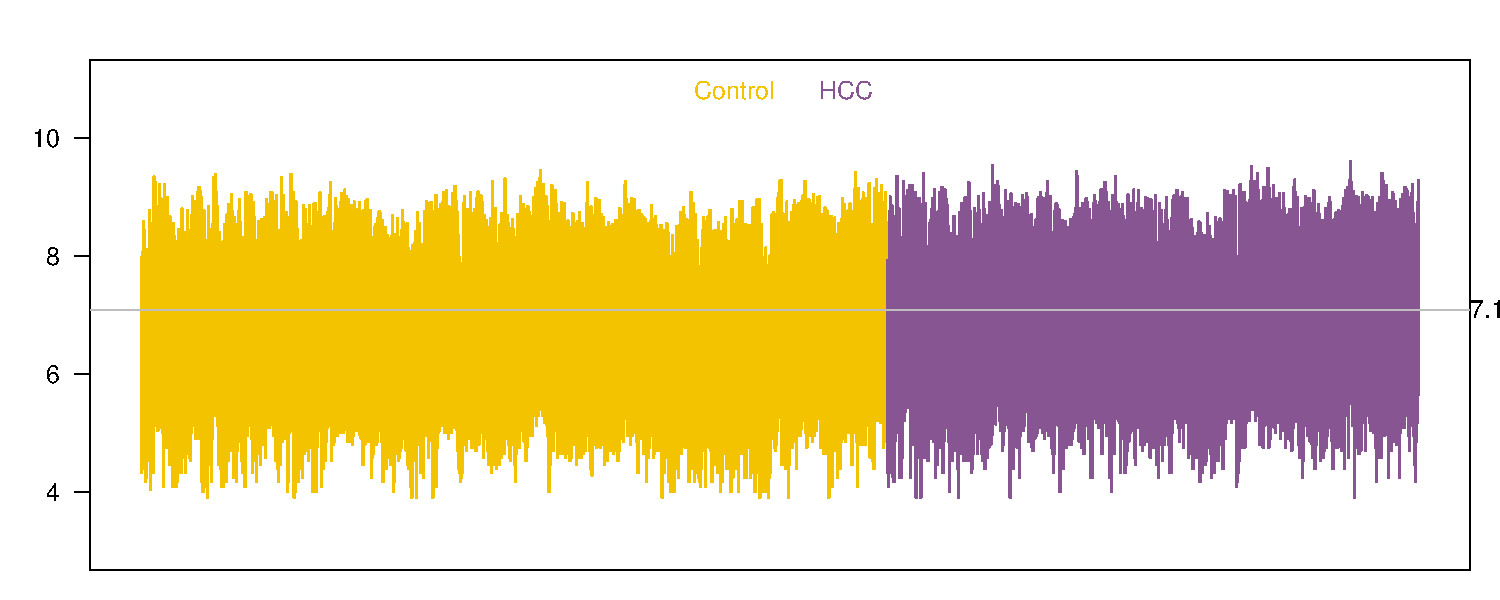
\includegraphics{Static/figures/lcpmBxp-1.pdf}
\caption{\label{fig:lcpmBxp}Sample log2 count boxplots}
\end{figure}

\begin{Shaded}
\begin{Highlighting}[]
\NormalTok{featureCountsA\_quant <{-}}\StringTok{ }\KeywordTok{apply}\NormalTok{(featureCountsA, }\DecValTok{2}\NormalTok{, }\ControlFlowTok{function}\NormalTok{(CC) \{}
  \KeywordTok{c}\NormalTok{(}\KeywordTok{quantile}\NormalTok{(CC, }\DataTypeTok{prob =} \KeywordTok{c}\NormalTok{(.}\DecValTok{15}\NormalTok{, (}\DecValTok{1}\OperatorTok{:}\DecValTok{3}\NormalTok{) }\OperatorTok{/}\StringTok{ }\DecValTok{4}\NormalTok{)), }\DataTypeTok{totCovM =} \KeywordTok{sum}\NormalTok{(CC) }\OperatorTok{/}\StringTok{ }\FloatTok{1e6}\NormalTok{)}
\NormalTok{\})}

\NormalTok{featureCountsA\_quant2 <{-}}\StringTok{ }\KeywordTok{apply}\NormalTok{(featureCountsA\_quant, }\DecValTok{1}\NormalTok{, }\ControlFlowTok{function}\NormalTok{(RR) \{}
  \KeywordTok{quantile}\NormalTok{(RR, }\DataTypeTok{prob =}\NormalTok{ (}\DecValTok{1}\OperatorTok{:}\DecValTok{3}\NormalTok{) }\OperatorTok{/}\StringTok{ }\DecValTok{4}\NormalTok{)}
\NormalTok{\})}

\NormalTok{knitr}\OperatorTok{::}\KeywordTok{kable}\NormalTok{(featureCountsA\_quant2,}
  \DataTypeTok{digits =} \DecValTok{1}\NormalTok{,}
  \DataTypeTok{caption =} \KeywordTok{paste}\NormalTok{(}
    \StringTok{"Coverage Summary {-} Columns are sample coverage quantiles and total coverage"}\NormalTok{,}
    \StringTok{"}\CharTok{\textbackslash{}n}\StringTok{Rows are quartiles across samples"}
\NormalTok{  )}
\NormalTok{) }\OperatorTok{\%>\%}\StringTok{ }\NormalTok{kableExtra}\OperatorTok{::}\KeywordTok{kable\_styling}\NormalTok{(}\DataTypeTok{full\_width =}\NormalTok{ F)}
\end{Highlighting}
\end{Shaded}

\begin{table}

\caption{\label{tab:quantCountsA}Coverage Summary - Columns are sample coverage quantiles and total coverage 
Rows are quartiles across samples}
\centering
\begin{tabular}[t]{l|r|r|r|r|r}
\hline
  & 15\% & 25\% & 50\% & 75\% & totCovM\\
\hline
25\% & 4 & 24 & 111 & 321 & 5.5\\
\hline
50\% & 5 & 30 & 135 & 391 & 6.7\\
\hline
75\% & 6 & 35 & 162 & 468 & 8.0\\
\hline
\end{tabular}
\end{table}

From this table, we see that 25\% of the samples have total coverage exceeding
\(8\)M reads, 25\% of samples
have a 15 percentile of coverage lower than
\(4\), etc.

\hypertarget{dra}{%
\section{Differential representation analysis}\label{dra}}

In the remainder of this section, we will process the data and
perform differential expression analysis as outlined in
Law et al.~(2018) {[}\protect\hyperlink{ref-Law:2018aa}{18}{]}. The main analysis steps are:

\begin{itemize}
\tightlist
\item
  remove lowly expressed genes
\item
  normalize gene expression distributions
\item
  remove heteroscedascity
\item
  fit linear models and examine DE results
\end{itemize}

It is good practice to perform this differential expression analysis prior to
fitting models to get an idea of how difficult it will be to discriminate
between samples belonging to the different subgroups. The pipeline
outlined in Law et al.~(2018) {[}\protect\hyperlink{ref-Law:2018aa}{18}{]} also provides some
basic quality assessment opportunities.

\hypertarget{remove-lowly-expressed-genes}{%
\subsection*{Remove lowly expressed genes}\label{remove-lowly-expressed-genes}}
\addcontentsline{toc}{subsection}{Remove lowly expressed genes}

Genes that are not expressed at a biologically
meaningful level in any condition should be discarded to reduce the
subset of genes to those that are of interest, and to reduce the number of tests
carried out downstream when looking at differential expression. Carrying
un-informative genes may also be a hindrance to classification and other
downtream analyses.

To determine a sensible threshold we can begin by examining the shapes of the distributions.

\begin{Shaded}
\begin{Highlighting}[]
\KeywordTok{par}\NormalTok{(}\DataTypeTok{mar =} \KeywordTok{c}\NormalTok{(}\DecValTok{4}\NormalTok{, }\DecValTok{3}\NormalTok{, }\DecValTok{2}\NormalTok{, }\DecValTok{1}\NormalTok{))}
\KeywordTok{plot}\NormalTok{(}\KeywordTok{density}\NormalTok{(lcpm\_mtx[, }\DecValTok{1}\NormalTok{]),}
  \DataTypeTok{col =}\NormalTok{ groupCol[sampDescA}\OperatorTok{$}\NormalTok{group[}\DecValTok{1}\NormalTok{]],}
  \DataTypeTok{lwd =} \DecValTok{2}\NormalTok{, }\DataTypeTok{ylim =} \KeywordTok{c}\NormalTok{(}\DecValTok{0}\NormalTok{, }\FloatTok{.25}\NormalTok{), }\DataTypeTok{las =} \DecValTok{2}\NormalTok{, }\DataTypeTok{main =} \StringTok{""}\NormalTok{, }\DataTypeTok{xlab =} \StringTok{"log2 CPM"}
\NormalTok{)}
\KeywordTok{abline}\NormalTok{(}\DataTypeTok{v =} \DecValTok{0}\NormalTok{, }\DataTypeTok{col =} \DecValTok{3}\NormalTok{)}
\CommentTok{\# After verifying no outliers, can plot a random subset }
\ControlFlowTok{for}\NormalTok{ (JJ }\ControlFlowTok{in} \KeywordTok{sample}\NormalTok{(}\DecValTok{2}\OperatorTok{:}\KeywordTok{ncol}\NormalTok{(lcpm\_mtx), }\DataTypeTok{size =} \DecValTok{100}\NormalTok{)) \{}
\NormalTok{  den <{-}}\StringTok{ }\KeywordTok{density}\NormalTok{(lcpm\_mtx[, JJ])}
  \KeywordTok{lines}\NormalTok{(den}\OperatorTok{$}\NormalTok{x, den}\OperatorTok{$}\NormalTok{y, }\DataTypeTok{col =}\NormalTok{ groupCol[sampDescA}\OperatorTok{$}\NormalTok{group[JJ]], }\DataTypeTok{lwd =} \DecValTok{2}\NormalTok{)}
\NormalTok{\} }\CommentTok{\# for(JJ}
\KeywordTok{legend}\NormalTok{(}\StringTok{"topright"}\NormalTok{, }\DataTypeTok{legend =} \KeywordTok{names}\NormalTok{(groupCol), }
  \DataTypeTok{text.col =}\NormalTok{ groupCol, }\DataTypeTok{bty =} \StringTok{"n"}\NormalTok{)}
\end{Highlighting}
\end{Shaded}

\begin{figure}
\centering
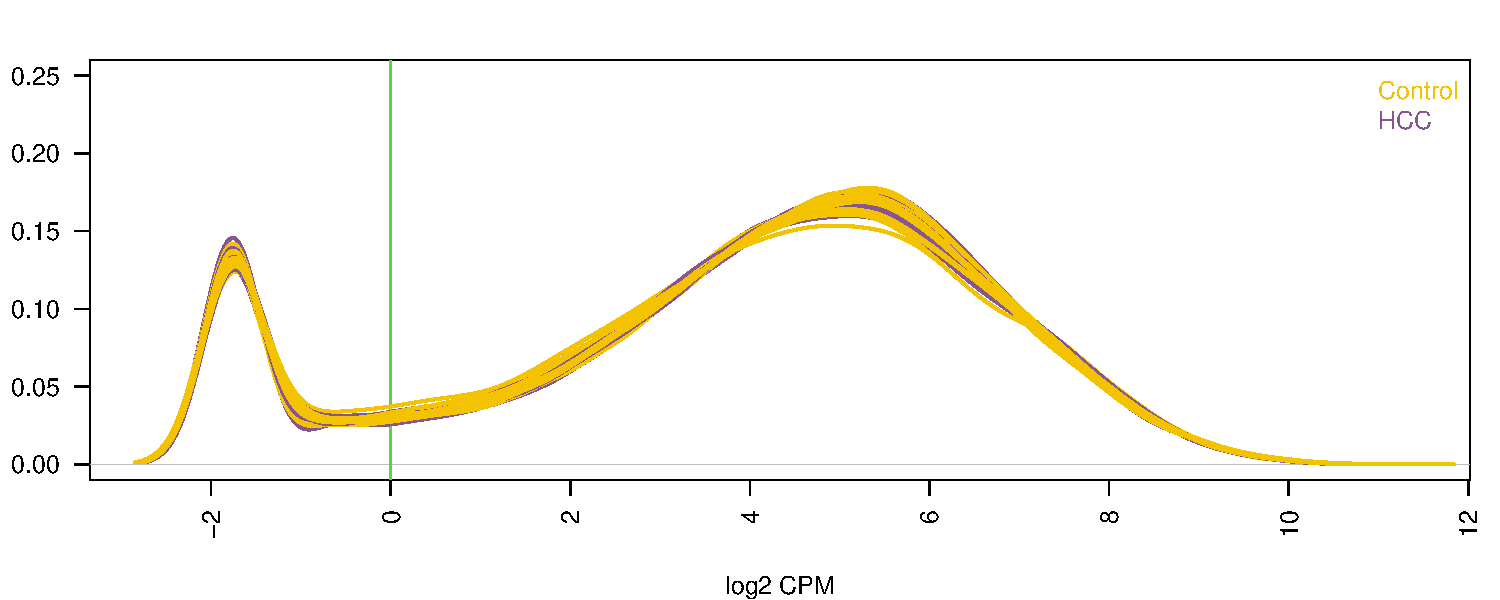
\includegraphics{Static/figures/densityLcpm-1.pdf}
\caption{\label{fig:densityLcpm}Sample \(log_2\) CPM densities}
\end{figure}

\[
\]

As is typically the case with RNA-Seq data, we notice many weakly represented genes
in this dataset. A cpm value of 1 appears to adequatly separate
the expressed from the un-expressed genes, but we will be slightly more strict here
and require a CPM threshold of \(3\) . Using a nominal CPM value of
\(3\), genes are deeemed to be \texttt{represented} if their expression is
above this threshold, and not represented otherwise.
For this analysis we will require that genes be \texttt{represented} in at least
\(25\) samples across the entire dataset to be retained for downstream analysis.
Here, a CPM value of \(3\) means that a gene is represented if it
has at least \(9\) reads in the sample with the
lowest sequencing depth (library size \(2.9\) million).
Note that the thresholds used here are arbitrary as there are no hard and fast
rules to set these by.
The voom-plot, which is part of analyses done to remove heteroscedasticity,
can be examined to verify that the filtering performed is adequate.

Remove weakly represented genes and replot densities.

\$\$
Removing \(17.5\)\% of genes\ldots{}

\begin{Shaded}
\begin{Highlighting}[]
\KeywordTok{par}\NormalTok{(}\DataTypeTok{mar =} \KeywordTok{c}\NormalTok{(}\DecValTok{4}\NormalTok{, }\DecValTok{3}\NormalTok{, }\DecValTok{2}\NormalTok{, }\DecValTok{1}\NormalTok{))}
\KeywordTok{plot}\NormalTok{(}\KeywordTok{density}\NormalTok{(lcpm\_mtx[, }\DecValTok{1}\NormalTok{]),}
  \DataTypeTok{col =}\NormalTok{ groupCol[sampDescA}\OperatorTok{$}\NormalTok{group[}\DecValTok{1}\NormalTok{]],}
  \DataTypeTok{lwd =} \DecValTok{2}\NormalTok{, }\DataTypeTok{ylim =} \KeywordTok{c}\NormalTok{(}\DecValTok{0}\NormalTok{, }\FloatTok{.25}\NormalTok{), }\DataTypeTok{las =} \DecValTok{2}\NormalTok{, }\DataTypeTok{main =} \StringTok{""}\NormalTok{, }\DataTypeTok{xlab =} \StringTok{"log2 CPM"}
\NormalTok{)}
\CommentTok{\#abline(v = 0, col = 3)}
\CommentTok{\# After verifying no outliers, can plot a random subset }
\ControlFlowTok{for}\NormalTok{ (JJ }\ControlFlowTok{in} \KeywordTok{sample}\NormalTok{(}\DecValTok{2}\OperatorTok{:}\KeywordTok{ncol}\NormalTok{(lcpm\_mtx), }\DataTypeTok{size =} \DecValTok{100}\NormalTok{)) \{}
\NormalTok{  den <{-}}\StringTok{ }\KeywordTok{density}\NormalTok{(lcpm\_mtx[, JJ])}
  \KeywordTok{lines}\NormalTok{(den}\OperatorTok{$}\NormalTok{x, den}\OperatorTok{$}\NormalTok{y, }\DataTypeTok{col =}\NormalTok{ groupCol[sampDescA}\OperatorTok{$}\NormalTok{group[JJ]], }\DataTypeTok{lwd =} \DecValTok{2}\NormalTok{)}
\NormalTok{\} }\CommentTok{\# for(JJ}
\KeywordTok{legend}\NormalTok{(}\StringTok{"topright"}\NormalTok{, }\DataTypeTok{legend =} \KeywordTok{names}\NormalTok{(groupCol), }
  \DataTypeTok{text.col =}\NormalTok{ groupCol, }\DataTypeTok{bty =} \StringTok{"n"}\NormalTok{)}
\end{Highlighting}
\end{Shaded}

\begin{figure}
\centering
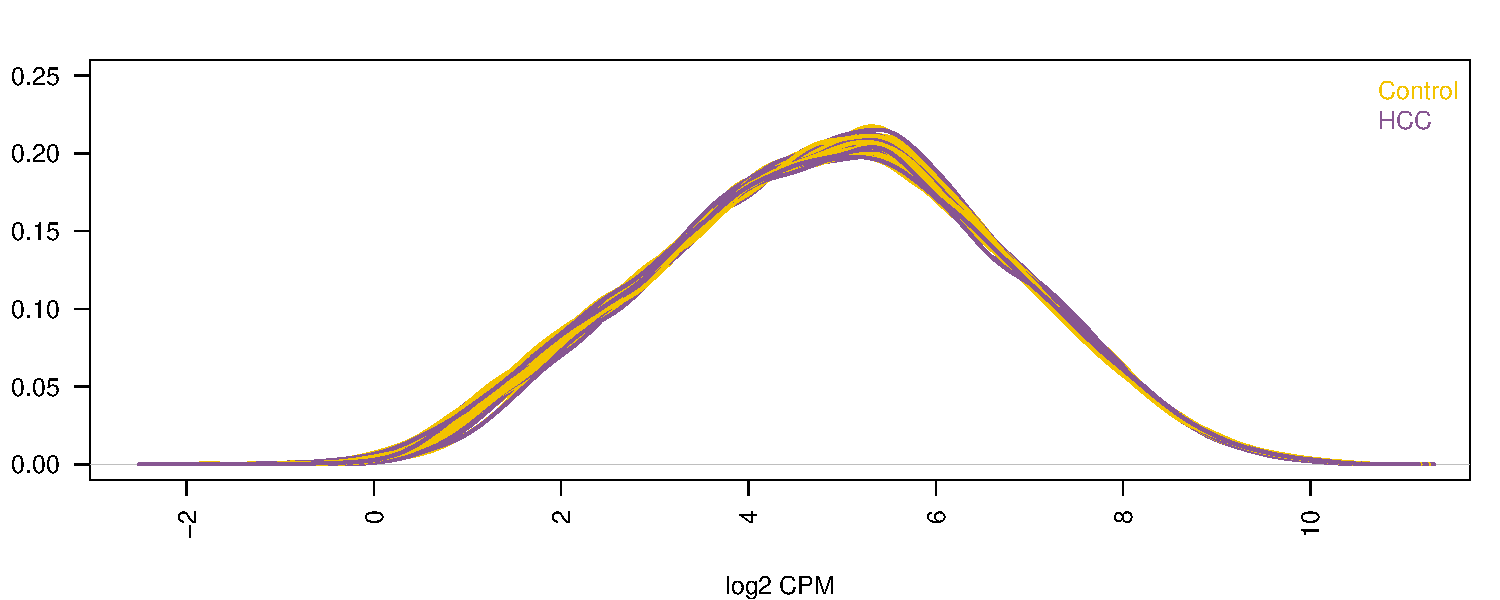
\includegraphics{Static/figures/densityLcpm2-1.pdf}
\caption{\label{fig:densityLcpm2}Sample \(log_2\) CPM densities after removing weak genes}
\end{figure}

As another sanity check, we will look at a
multidimensional scaling plot of distances between gene expression
profiles. We use \texttt{plotMDS} in limma package {[}\protect\hyperlink{ref-Ritchie:2015aa}{19}{]}),
which plots samples on a two-dimensional scatterplot so that distances on
the plot approximate the typical log2 fold changes between the
samples.

Before producing the MDS plot we will normalize the distributions.
We will store the data into s \texttt{DGEList} object as this is convenient
when running many of the analyses implemented in the edgeR and limma packages.
Call the set `AF', for set `A', `Filtered'.

\begin{Shaded}
\begin{Highlighting}[]
\NormalTok{AF\_dgel <{-}}\StringTok{ }\NormalTok{edgeR}\OperatorTok{::}\KeywordTok{DGEList}\NormalTok{(}
  \DataTypeTok{counts =}\NormalTok{ featureCountsAF,}
  \DataTypeTok{genes =}\NormalTok{ genes\_annotAF,}
  \DataTypeTok{samples =}\NormalTok{ sampDescA,}
  \DataTypeTok{group =}\NormalTok{ sampDescA}\OperatorTok{$}\NormalTok{group}
\NormalTok{)}
\NormalTok{AF\_dgel <{-}}\StringTok{ }\NormalTok{edgeR}\OperatorTok{::}\KeywordTok{calcNormFactors}\NormalTok{(AF\_dgel)}
\NormalTok{AF\_lcmp\_mtx <{-}}\StringTok{ }\NormalTok{edgeR}\OperatorTok{::}\KeywordTok{cpm}\NormalTok{(AF\_dgel, }\DataTypeTok{log =}\NormalTok{ T)}

\CommentTok{\# Save AF\_dgel to facilitate restarting}
\CommentTok{\# remove from final version}
\KeywordTok{save}\NormalTok{(}\DataTypeTok{list =} \StringTok{"AF\_dgel"}\NormalTok{, }\DataTypeTok{file =} \StringTok{"RData/AF\_dgel"}\NormalTok{)}
\end{Highlighting}
\end{Shaded}

Verify that the counts are properly normalized.

\begin{Shaded}
\begin{Highlighting}[]
\KeywordTok{par}\NormalTok{(}\DataTypeTok{mar =} \KeywordTok{c}\NormalTok{(}\DecValTok{1}\NormalTok{, }\DecValTok{3}\NormalTok{, }\DecValTok{2}\NormalTok{, }\DecValTok{1}\NormalTok{))}
\KeywordTok{boxplot}\NormalTok{(AF\_lcmp\_mtx,}
  \DataTypeTok{ylim =} \KeywordTok{c}\NormalTok{(}\DecValTok{1}\NormalTok{, }\DecValTok{8}\NormalTok{), }\DataTypeTok{ylab=}\StringTok{\textquotesingle{}Normalized Log CPM\textquotesingle{}}\NormalTok{,}
  \DataTypeTok{staplewex =} \DecValTok{0}\NormalTok{,       }\CommentTok{\# remove horizontal whisker lines}
  \DataTypeTok{staplecol =} \StringTok{"white"}\NormalTok{, }\CommentTok{\# just to be totally sure :)}
  \DataTypeTok{outline =}\NormalTok{ F,         }\CommentTok{\# remove outlying points}
  \DataTypeTok{whisklty =} \DecValTok{0}\NormalTok{,        }\CommentTok{\# remove vertical whisker lines}
  \DataTypeTok{las =} \DecValTok{2}\NormalTok{, }\DataTypeTok{horizontal =}\NormalTok{ F, }\DataTypeTok{xaxt =} \StringTok{"n"}\NormalTok{,}
  \DataTypeTok{border =}\NormalTok{ groupCol[sampDescA}\OperatorTok{$}\NormalTok{group]}
\NormalTok{)}
\KeywordTok{legend}\NormalTok{(}\StringTok{"top"}\NormalTok{, }\DataTypeTok{legend =} \KeywordTok{names}\NormalTok{(groupCol), }\DataTypeTok{text.col =}\NormalTok{ groupCol,}
  \DataTypeTok{ncol =} \DecValTok{2}\NormalTok{, }\DataTypeTok{bty =} \StringTok{"n"}\NormalTok{)}
\CommentTok{\# Add reference lines}
\NormalTok{SampleMedian <{-}}\StringTok{ }\KeywordTok{apply}\NormalTok{(AF\_lcmp\_mtx, }\DecValTok{2}\NormalTok{, median)}
\KeywordTok{abline}\NormalTok{(}\DataTypeTok{h =} \KeywordTok{median}\NormalTok{(SampleMedian), }\DataTypeTok{col =} \StringTok{"grey"}\NormalTok{)}
\KeywordTok{axis}\NormalTok{(}\DataTypeTok{side =} \DecValTok{4}\NormalTok{, }\DataTypeTok{at =} \KeywordTok{round}\NormalTok{(}\KeywordTok{median}\NormalTok{(SampleMedian), }\DecValTok{1}\NormalTok{),}
  \DataTypeTok{las =} \DecValTok{2}\NormalTok{, }\DataTypeTok{col =} \StringTok{"grey"}\NormalTok{, }\DataTypeTok{line =} \DecValTok{{-}1}\NormalTok{, }\DataTypeTok{tick =}\NormalTok{ F)}
\end{Highlighting}
\end{Shaded}

\begin{figure}
\centering
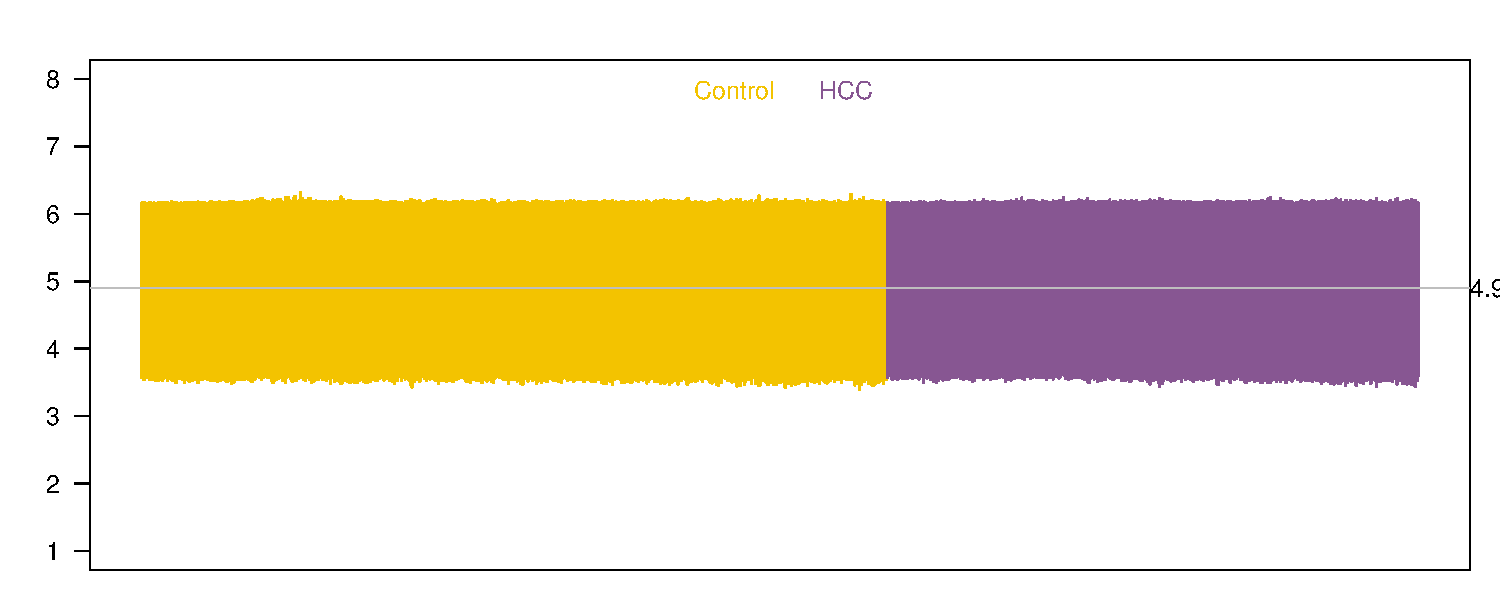
\includegraphics{Static/figures/normedLcpmBxp-1.pdf}
\caption{\label{fig:normedLcpmBxp}Sample log2 count boxplots}
\end{figure}

Proceed with MDS plots.

\begin{Shaded}
\begin{Highlighting}[]
\KeywordTok{par}\NormalTok{(}\DataTypeTok{mfcol =} \KeywordTok{c}\NormalTok{(}\DecValTok{1}\NormalTok{, }\DecValTok{2}\NormalTok{), }\DataTypeTok{mar =} \KeywordTok{c}\NormalTok{(}\DecValTok{4}\NormalTok{, }\DecValTok{4}\NormalTok{, }\DecValTok{2}\NormalTok{, }\DecValTok{1}\NormalTok{), }\DataTypeTok{xpd =} \OtherTok{NA}\NormalTok{, }\DataTypeTok{oma =} \KeywordTok{c}\NormalTok{(}\DecValTok{0}\NormalTok{, }\DecValTok{0}\NormalTok{, }\DecValTok{2}\NormalTok{, }\DecValTok{0}\NormalTok{))}

\CommentTok{\# wo loss of generality, sample 500 samples}
\CommentTok{\# simply a matter of convenience to save time}
\CommentTok{\# remove from final version}
\KeywordTok{set.seed}\NormalTok{(}\DecValTok{1}\NormalTok{)}
\NormalTok{samp\_ndx <{-}}\StringTok{ }\KeywordTok{sample}\NormalTok{(}\DecValTok{1}\OperatorTok{:}\KeywordTok{ncol}\NormalTok{(AF\_lcmp\_mtx), }\DataTypeTok{size =} \DecValTok{500}\NormalTok{)}
\NormalTok{MDS.out <{-}}\StringTok{ }\NormalTok{limma}\OperatorTok{::}\KeywordTok{plotMDS}\NormalTok{(AF\_lcmp\_mtx[, samp\_ndx],}
  \DataTypeTok{col =}\NormalTok{ groupCol[sampDescA}\OperatorTok{$}\NormalTok{group[samp\_ndx]], }\DataTypeTok{pch =} \DecValTok{1}
\NormalTok{)}
\KeywordTok{legend}\NormalTok{(}\StringTok{"topleft"}\NormalTok{,}
  \DataTypeTok{legend =} \KeywordTok{names}\NormalTok{(groupCol),}
  \DataTypeTok{text.col =}\NormalTok{ groupCol, }\DataTypeTok{bty =} \StringTok{"n"}
\NormalTok{)}

\NormalTok{MDS.out <{-}}\StringTok{ }\NormalTok{limma}\OperatorTok{::}\KeywordTok{plotMDS}\NormalTok{(AF\_lcmp\_mtx[, samp\_ndx],}
  \DataTypeTok{col =}\NormalTok{ groupCol[sampDescA}\OperatorTok{$}\NormalTok{group[samp\_ndx]], }\DataTypeTok{pch =} \DecValTok{1}\NormalTok{,}
  \DataTypeTok{dim.plot =} \DecValTok{3}\OperatorTok{:}\DecValTok{4}
\NormalTok{)}
\end{Highlighting}
\end{Shaded}

\begin{figure}
\centering
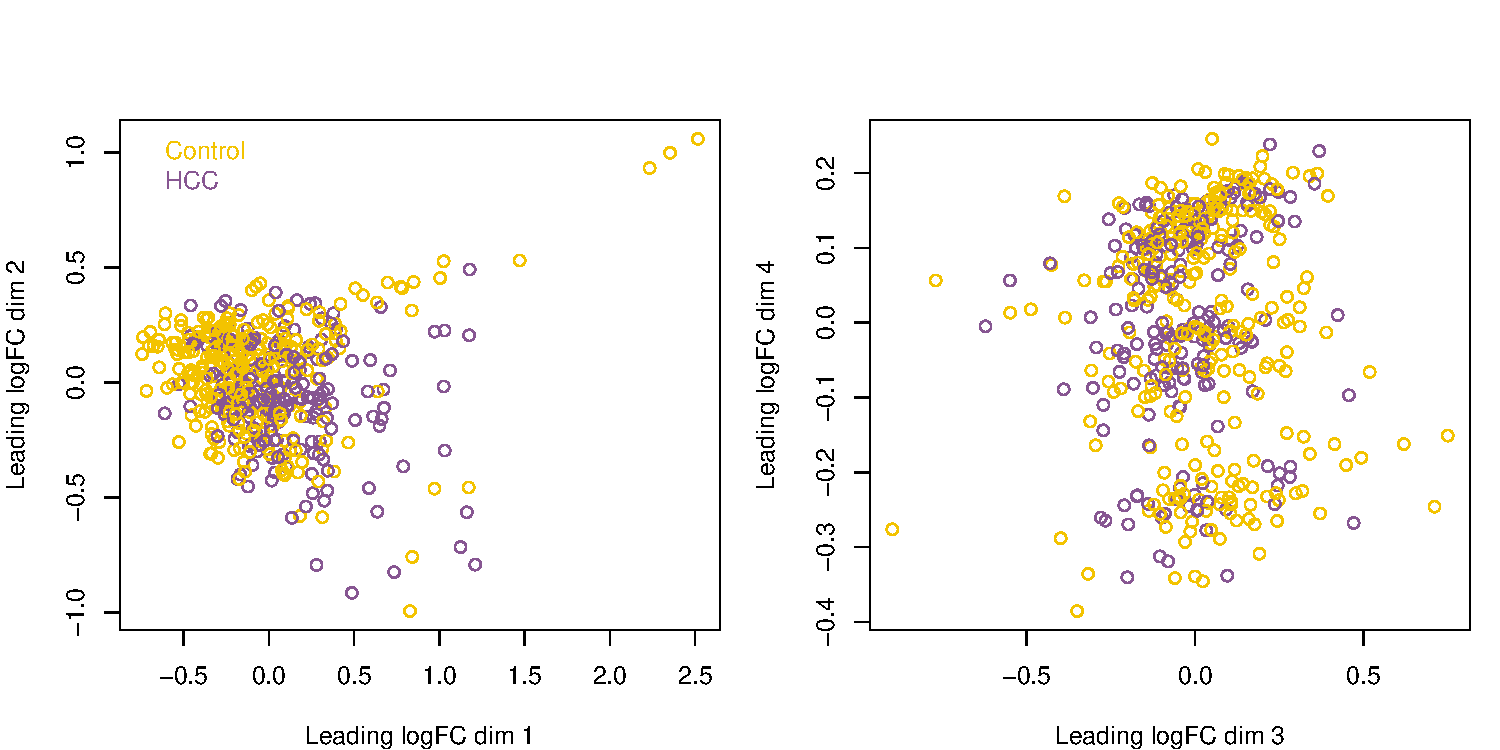
\includegraphics{Static/figures/plotMDS-1.pdf}
\caption{\label{fig:plotMDS}MDS plots of log-CPM values}
\end{figure}

The MDS plot, which is analogous to a PCA plot adapted to gene exression data,
does not indicate strong clustering of samples. The fanning pattern observed in the
first two dimensions indicates that a few samples are drifting way from the
core set, but in no particular direction. There is some structure in the
3rd and 4th dimension plot which should be investigated.\\
\texttt{glMDSPlot} from package \texttt{Glimma} provides an interactive MDS
plot that can extremely usful for exploration

\begin{Shaded}
\begin{Highlighting}[]
\NormalTok{Glimma}\OperatorTok{::}\KeywordTok{glMDSPlot}\NormalTok{(AF\_dgel[, samp\_ndx],}
  \DataTypeTok{groups =}\NormalTok{ AF\_dgel}\OperatorTok{$}\NormalTok{samples[}
\NormalTok{    samp\_ndx,}
    \KeywordTok{c}\NormalTok{(}\StringTok{"group"}\NormalTok{, }\StringTok{"trainValGroup"}\NormalTok{, }\StringTok{"sampType"}\NormalTok{, }\StringTok{"tissue"}\NormalTok{, }\StringTok{"title"}\NormalTok{, }\StringTok{"stage"}\NormalTok{)}
\NormalTok{  ],}
  \DataTypeTok{main =} \KeywordTok{paste}\NormalTok{(}\StringTok{"MDS plot: filtered counts"}\NormalTok{), }\CommentTok{\#\#\#\# , Excluding outlier samples"),}
  \DataTypeTok{path =} \StringTok{"."}\NormalTok{, }\DataTypeTok{folder =}\NormalTok{ figures\_DIR,}
  \DataTypeTok{html =} \KeywordTok{paste0}\NormalTok{(}\StringTok{"GlMDSplot"}\NormalTok{), }\DataTypeTok{launch =}\NormalTok{ F}
\NormalTok{)}
\end{Highlighting}
\end{Shaded}

Link to glMDSPlot:
\href{$Static/figures//GlMDSplot.html$}{Here}

No obvious factor links the samples in the 3 clusters observed on the
4th MDS dimensions. The percent of variance exaplained by this dimension or
\(\approx\) 4\%. The glMDSPlot indicates further segregation along
the 6th dimension. The percent of variance exaplained by this dimension or
\(\approx\) 2\%. Tracking down this source of variability may be quite challenging,
especially without having the complete information about the sample attributes
and provenance.

Unwanted variability is a well-documented problem in the analysis of RNA-Seq data
(see Peixoto et al.~(2015) {[}\protect\hyperlink{ref-Peixoto:2015aa}{20}{]}), and many procedures have been proposed
to reduce the effect of unwanted variation on RNA-Seq analsys results
({[}\protect\hyperlink{ref-Peixoto:2015aa}{20}--\protect\hyperlink{ref-Risso:2014aa}{22}{]}). There are undoubtedly
some similar sources of systematic variation in the 5hmC data, but it is
beyond the scope of this work to investigate these in this particular dataset.
Given that the clustering of samples occurs in MDS dimensions that explain
a small fraction of variability, and that these is no assocation with the
factor of interest, HCC vs Control, these sources of variability should not
interfere too much with our classification analysis. It would nonetheless be interesting
to assess whether downstream results can be improved by removing this variability.

\hypertarget{creating-a-design-matrix-and-contrasts}{%
\subsection*{Creating a design matrix and contrasts}\label{creating-a-design-matrix-and-contrasts}}
\addcontentsline{toc}{subsection}{Creating a design matrix and contrasts}

Before proceeding with the statistical modeling used for the
differential expression analysis, we need to set up a
model design matrix.

\begin{Shaded}
\begin{Highlighting}[]
\NormalTok{Design\_mtx <{-}}\StringTok{ }\KeywordTok{model.matrix}\NormalTok{( }\OperatorTok{\textasciitilde{}}\StringTok{  }\DecValTok{{-}1} \OperatorTok{+}\StringTok{ }\NormalTok{group, }\DataTypeTok{data=}\NormalTok{AF\_dgel}\OperatorTok{$}\NormalTok{samples)}
\KeywordTok{colnames}\NormalTok{(Design\_mtx) <{-}}\StringTok{ }\KeywordTok{sub}\NormalTok{(}\StringTok{\textquotesingle{}group\textquotesingle{}}\NormalTok{, }\StringTok{\textquotesingle{}\textquotesingle{}}\NormalTok{, }\KeywordTok{colnames}\NormalTok{(Design\_mtx))}

\KeywordTok{cat}\NormalTok{(}\StringTok{"colSums(Design\_mtx):}\CharTok{\textbackslash{}n}\StringTok{"}\NormalTok{)}
\end{Highlighting}
\end{Shaded}

\begin{verbatim}
## colSums(Design_mtx):
\end{verbatim}

\begin{Shaded}
\begin{Highlighting}[]
\KeywordTok{colSums}\NormalTok{(Design\_mtx)}
\end{Highlighting}
\end{Shaded}

\begin{verbatim}
## Control     HCC 
##     778     555
\end{verbatim}

\begin{Shaded}
\begin{Highlighting}[]
\NormalTok{Contrasts\_mtx <{-}}\StringTok{ }\NormalTok{limma}\OperatorTok{::}\KeywordTok{makeContrasts}\NormalTok{(}
  \DataTypeTok{HCCvsControl =}\NormalTok{ HCC  }\OperatorTok{{-}}\StringTok{ }\NormalTok{Control,}
  \DataTypeTok{levels=}\KeywordTok{colnames}\NormalTok{(Design\_mtx))}

\KeywordTok{cat}\NormalTok{(}\StringTok{"Contrasts:}\CharTok{\textbackslash{}n}\StringTok{"}\NormalTok{)}
\end{Highlighting}
\end{Shaded}

\begin{verbatim}
## Contrasts:
\end{verbatim}

\begin{Shaded}
\begin{Highlighting}[]
\NormalTok{Contrasts\_mtx}
\end{Highlighting}
\end{Shaded}

\begin{verbatim}
##          Contrasts
## Levels    HCCvsControl
##   Control           -1
##   HCC                1
\end{verbatim}

\hypertarget{removing-heteroscedasticity-from-the-count-data}{%
\subsection*{Removing heteroscedasticity from the count data}\label{removing-heteroscedasticity-from-the-count-data}}
\addcontentsline{toc}{subsection}{Removing heteroscedasticity from the count data}

As for RNA-Seq data, for 5hmC count data the variance is not independent of the mean.
In \texttt{limma}, the R package we are using for our analyses,
linear modeling is carried out on the log-CPM values which are assumed to be
normally distributed and the mean-variance relationship is accommodated using precision
weights calculated by the voom function. We apply this transformation next.

\begin{Shaded}
\begin{Highlighting}[]
\KeywordTok{par}\NormalTok{(}\DataTypeTok{mfrow=}\KeywordTok{c}\NormalTok{(}\DecValTok{1}\NormalTok{,}\DecValTok{1}\NormalTok{))}
\NormalTok{filteredCountsAF\_voom <{-}}\StringTok{ }\NormalTok{limma}\OperatorTok{::}\KeywordTok{voom}\NormalTok{(AF\_dgel, Design\_mtx, }\DataTypeTok{plot=}\NormalTok{T)}
\end{Highlighting}
\end{Shaded}

\begin{figure}
\centering
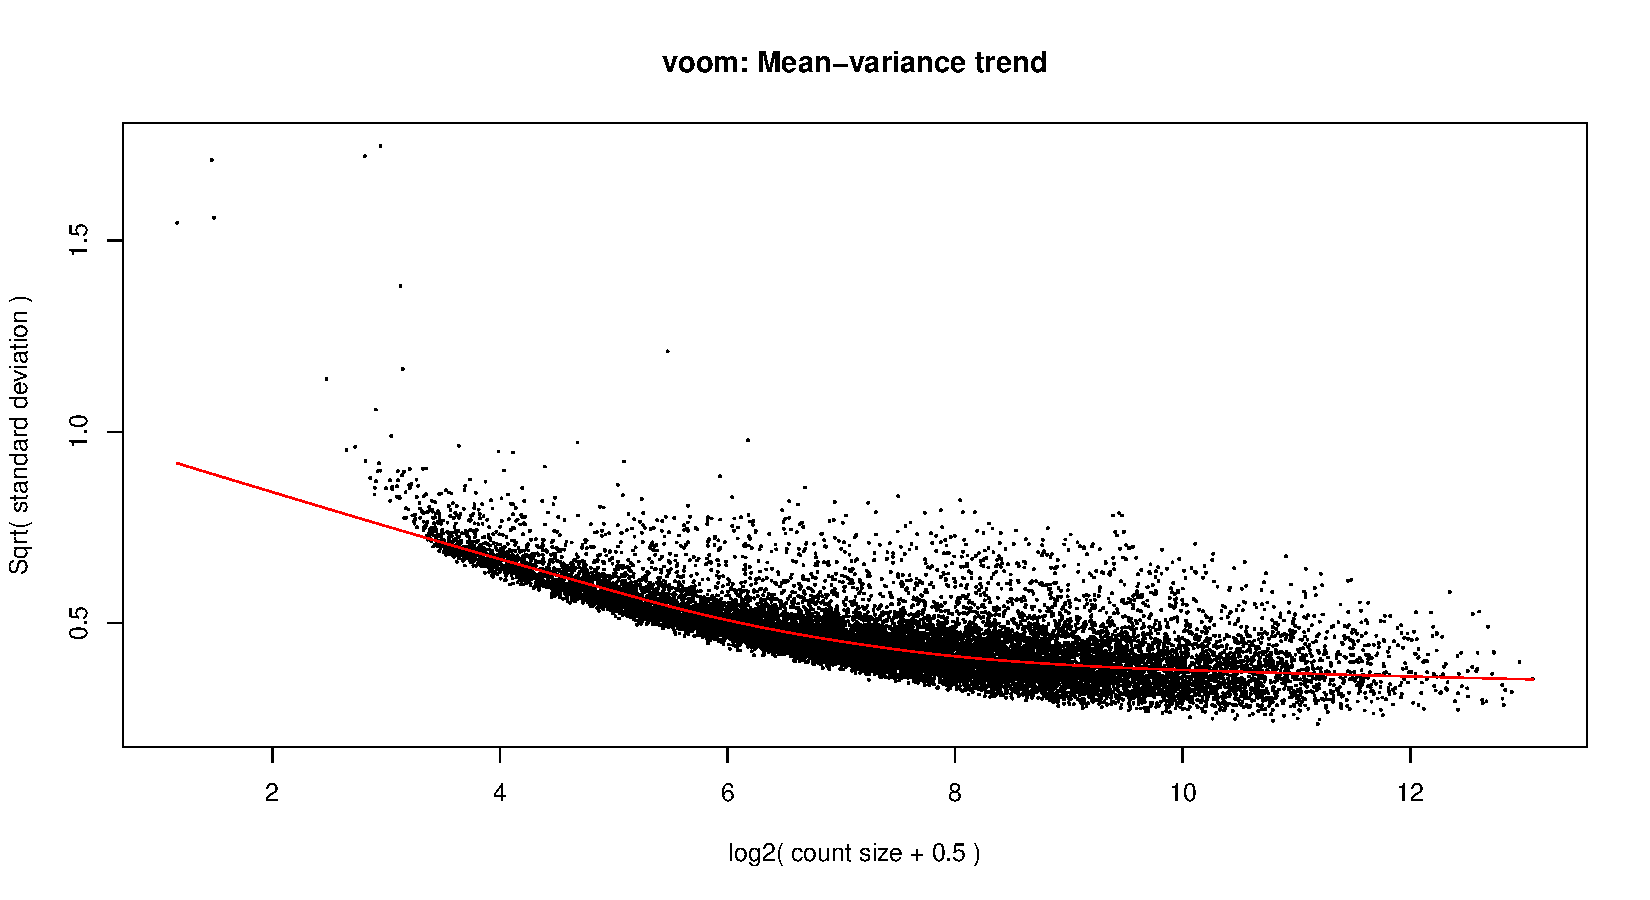
\includegraphics{Static/figures/Voom1-1.pdf}
\caption{\label{fig:Voom1}Removing heteroscedascity}
\end{figure}

Note that the voom-plot provides a visual check on the level of filtering performed upstream.
If filtering of lowly-expressed genes is insufficient, a drop in variance levels can be
observed at the low end of the expression scale due to very small counts.

\hypertarget{fit-linear-models-and-examine-the-results}{%
\subsection*{Fit linear models and examine the results}\label{fit-linear-models-and-examine-the-results}}
\addcontentsline{toc}{subsection}{Fit linear models and examine the results}

Having properly filtered and normalized the data,
the linear models can be fitted to each gene and the results
examined to assess differential expression between the two groups
of interest, in our case HCC vs Control.

Table \ref{tab:lmFit} displays the counts of genes in each DE category:

\begin{Shaded}
\begin{Highlighting}[]
\NormalTok{ filteredCountsAF\_voom\_fit <{-}}\StringTok{ }\NormalTok{limma}\OperatorTok{::}\KeywordTok{lmFit}\NormalTok{(filteredCountsAF\_voom, Design\_mtx)}
 \KeywordTok{colnames}\NormalTok{(filteredCountsAF\_voom\_fit}\OperatorTok{$}\NormalTok{coefficients) <{-}}\StringTok{ }\KeywordTok{sub}\NormalTok{(}\StringTok{"}\CharTok{\textbackslash{}\textbackslash{}}\StringTok{(Intercept}\CharTok{\textbackslash{}\textbackslash{}}\StringTok{)"}\NormalTok{, }\StringTok{"Intercept"}\NormalTok{,}
 \KeywordTok{colnames}\NormalTok{(filteredCountsAF\_voom\_fit}\OperatorTok{$}\NormalTok{coefficients) )}

\NormalTok{ filteredCountsAF\_voom\_fit <{-}}\StringTok{ }\NormalTok{limma}\OperatorTok{::}\KeywordTok{contrasts.fit}\NormalTok{(}
\NormalTok{    filteredCountsAF\_voom\_fit, }\DataTypeTok{contrasts=}\NormalTok{Contrasts\_mtx)}

\NormalTok{ filteredCountsAF\_voom\_efit <{-}}\StringTok{ }\NormalTok{limma}\OperatorTok{::}\KeywordTok{eBayes}\NormalTok{(filteredCountsAF\_voom\_fit)}

\NormalTok{ filteredCountsAF\_voom\_efit\_dt <{-}}
\StringTok{ }\NormalTok{limma}\OperatorTok{::}\KeywordTok{decideTests}\NormalTok{(filteredCountsAF\_voom\_efit,}\DataTypeTok{adjust.method =} \StringTok{"BH"}\NormalTok{, }\DataTypeTok{p.value =} \FloatTok{0.05}\NormalTok{)}
 
\NormalTok{ knitr}\OperatorTok{::}\KeywordTok{kable}\NormalTok{(}\KeywordTok{t}\NormalTok{(}\KeywordTok{summary}\NormalTok{(filteredCountsAF\_voom\_efit\_dt)),}
  \DataTypeTok{caption=}\StringTok{"DE Results at FDR = 0.05"}\NormalTok{) }\OperatorTok{\%>\%}\StringTok{ }
\StringTok{  }\NormalTok{kableExtra}\OperatorTok{::}\KeywordTok{kable\_styling}\NormalTok{(}\DataTypeTok{full\_width =}\NormalTok{ F)}
\end{Highlighting}
\end{Shaded}

\begin{table}

\caption{\label{tab:lmFit}DE Results at FDR = 0.05}
\centering
\begin{tabular}[t]{l|r|r|r}
\hline
  & Down & NotSig & Up\\
\hline
HCCvsControl & 5214 & 5280 & 5258\\
\hline
\end{tabular}
\end{table}

\hypertarget{graphical-representations-of-de-results-md-plots}{%
\subsection*{Graphical representations of DE results: MD Plots}\label{graphical-representations-of-de-results-md-plots}}
\addcontentsline{toc}{subsection}{Graphical representations of DE results: MD Plots}

To summarise results for all genes visually, mean-difference plots
(aka MA plot), which display log-FCs from the linear model fit against
the average log-CPM values can be generated using the plotMD function,
with the differentially expressed genes highlighted.

We may also be interested in whether certain gene features are
related to gene identification. Gene GC content, for example, might be
of interest.

\begin{Shaded}
\begin{Highlighting}[]
\KeywordTok{par}\NormalTok{(}\DataTypeTok{mfrow=}\KeywordTok{c}\NormalTok{(}\DecValTok{1}\NormalTok{,}\DecValTok{3}\NormalTok{), }\DataTypeTok{mar=}\KeywordTok{c}\NormalTok{(}\FloatTok{4.5}\NormalTok{,}\FloatTok{4.5}\NormalTok{,}\DecValTok{2}\NormalTok{,}\DecValTok{1}\NormalTok{),}\DataTypeTok{oma=}\KeywordTok{c}\NormalTok{(}\DecValTok{1}\NormalTok{,}\DecValTok{1}\NormalTok{,}\DecValTok{2}\NormalTok{,}\DecValTok{0}\NormalTok{))}

\CommentTok{\# log{-}fold{-}change vs ave{-}expr}
\NormalTok{limma}\OperatorTok{::}\KeywordTok{plotMD}\NormalTok{(filteredCountsAF\_voom\_efit,}
 \DataTypeTok{ylim =} \KeywordTok{c}\NormalTok{(}\OperatorTok{{-}}\FloatTok{0.4}\NormalTok{, }\FloatTok{0.4}\NormalTok{),}
 \DataTypeTok{column=}\StringTok{\textquotesingle{}HCCvsControl\textquotesingle{}}\NormalTok{,}
 \DataTypeTok{status=}\NormalTok{filteredCountsAF\_voom\_efit\_dt[,}\StringTok{\textquotesingle{}HCCvsControl\textquotesingle{}}\NormalTok{],}
 \DataTypeTok{hl.pch =} \DecValTok{16}\NormalTok{, }\DataTypeTok{hl.col =} \KeywordTok{c}\NormalTok{(}\StringTok{"lightblue"}\NormalTok{, }\StringTok{"pink"}\NormalTok{), }\DataTypeTok{hl.cex =} \FloatTok{.5}\NormalTok{,}
 \DataTypeTok{bg.pch =} \DecValTok{16}\NormalTok{, }\DataTypeTok{bg.col =} \StringTok{"grey"}\NormalTok{, }\DataTypeTok{bg.cex =} \FloatTok{0.5}\NormalTok{,}
 \DataTypeTok{main =} \StringTok{\textquotesingle{}\textquotesingle{}}\NormalTok{,}
 \DataTypeTok{xlab =} \KeywordTok{paste0}\NormalTok{(}
    \StringTok{"Average log{-}expression: IQR="}\NormalTok{,}
    \KeywordTok{paste}\NormalTok{(}\KeywordTok{round}\NormalTok{(}\KeywordTok{quantile}\NormalTok{(filteredCountsAF\_voom\_efit}\OperatorTok{$}\NormalTok{Amean, }\DataTypeTok{prob =} \KeywordTok{c}\NormalTok{(}\DecValTok{1}\NormalTok{, }\DecValTok{3}\NormalTok{) }\OperatorTok{/}\StringTok{ }\DecValTok{4}\NormalTok{), }\DecValTok{2}\NormalTok{),}
      \DataTypeTok{collapse =} \StringTok{", "}
\NormalTok{    )}
\NormalTok{  ),}
  \DataTypeTok{ylab =} \KeywordTok{paste0}\NormalTok{(}
    \StringTok{"log{-}fold{-}change: IQR="}\NormalTok{,}
    \KeywordTok{paste}\NormalTok{(}\KeywordTok{round}\NormalTok{(}\KeywordTok{quantile}\NormalTok{(filteredCountsAF\_voom\_efit}\OperatorTok{$}\NormalTok{coefficients[, }\StringTok{\textquotesingle{}HCCvsControl\textquotesingle{}}\NormalTok{], }\DataTypeTok{prob =} \KeywordTok{c}\NormalTok{(}\DecValTok{1}\NormalTok{, }\DecValTok{3}\NormalTok{) }\OperatorTok{/}\StringTok{ }\DecValTok{4}\NormalTok{), }\DecValTok{2}\NormalTok{),}
      \DataTypeTok{collapse =} \StringTok{", "}
\NormalTok{    )}
\NormalTok{  ),}
  \DataTypeTok{legend =}\NormalTok{ F, }\DataTypeTok{cex.lab=}\FloatTok{1.5}
\NormalTok{)}
\KeywordTok{abline}\NormalTok{(}\DataTypeTok{h =} \DecValTok{0}\NormalTok{, }\DataTypeTok{col =} \StringTok{"black"}\NormalTok{)}
\KeywordTok{rug}\NormalTok{(}\KeywordTok{quantile}\NormalTok{(filteredCountsAF\_voom\_efit}\OperatorTok{$}\NormalTok{coefficients[, }\StringTok{\textquotesingle{}HCCvsControl\textquotesingle{}}\NormalTok{], }\DataTypeTok{prob =} \KeywordTok{c}\NormalTok{(}\DecValTok{1}\NormalTok{, }\DecValTok{2}\NormalTok{, }\DecValTok{3}\NormalTok{) }\OperatorTok{/}\StringTok{ }\DecValTok{4}\NormalTok{),}
  \DataTypeTok{col =} \StringTok{"purple"}\NormalTok{,}
  \DataTypeTok{ticksize =} \FloatTok{.03}\NormalTok{, }\DataTypeTok{side =} \DecValTok{2}\NormalTok{, }\DataTypeTok{lwd =} \DecValTok{2}
\NormalTok{)}
\KeywordTok{rug}\NormalTok{(}\KeywordTok{quantile}\NormalTok{(filteredCountsAF\_voom\_efit}\OperatorTok{$}\NormalTok{Amean, }\DataTypeTok{prob =} \KeywordTok{c}\NormalTok{(}\DecValTok{1}\NormalTok{, }\DecValTok{2}\NormalTok{, }\DecValTok{3}\NormalTok{) }\OperatorTok{/}\StringTok{ }\DecValTok{4}\NormalTok{),}
  \DataTypeTok{col =} \StringTok{"purple"}\NormalTok{,}
  \DataTypeTok{ticksize =} \FloatTok{.03}\NormalTok{, }\DataTypeTok{side =} \DecValTok{1}\NormalTok{, }\DataTypeTok{lwd =} \DecValTok{2}
\NormalTok{)}

\CommentTok{\# log{-}fold{-}change vs identification}

\KeywordTok{boxplot}\NormalTok{(}\KeywordTok{split}\NormalTok{(}
\NormalTok{ filteredCountsAF\_voom\_efit}\OperatorTok{$}\NormalTok{coefficients[, }\StringTok{\textquotesingle{}HCCvsControl\textquotesingle{}}\NormalTok{],}
\NormalTok{ filteredCountsAF\_voom\_efit\_dt[,}\StringTok{\textquotesingle{}HCCvsControl\textquotesingle{}}\NormalTok{]),}
 \DataTypeTok{outline=}\NormalTok{F,}
 \DataTypeTok{border=}\KeywordTok{c}\NormalTok{(}\StringTok{"pink"}\NormalTok{, }\StringTok{"grey"}\NormalTok{, }\StringTok{"lightblue"}\NormalTok{), }\DataTypeTok{xaxt=}\StringTok{\textquotesingle{}n\textquotesingle{}}\NormalTok{,}
 \DataTypeTok{ylab=}\StringTok{\textquotesingle{}log{-}fold{-}change\textquotesingle{}}\NormalTok{, }\DataTypeTok{ylim=}\KeywordTok{c}\NormalTok{(}\OperatorTok{{-}}\NormalTok{.}\DecValTok{4}\NormalTok{, }\FloatTok{.4}\NormalTok{),}
 \DataTypeTok{cex.lab=}\FloatTok{1.5}
\NormalTok{)}
\KeywordTok{axis}\NormalTok{(}\DataTypeTok{side=}\DecValTok{1}\NormalTok{, }\DataTypeTok{at=}\DecValTok{1}\OperatorTok{:}\DecValTok{3}\NormalTok{, }\KeywordTok{c}\NormalTok{(}\StringTok{\textquotesingle{}down\textquotesingle{}}\NormalTok{, }\StringTok{\textquotesingle{}notDE\textquotesingle{}}\NormalTok{, }\StringTok{\textquotesingle{}up\textquotesingle{}}\NormalTok{), }\DataTypeTok{cex.axis=}\FloatTok{1.5}\NormalTok{)}

\CommentTok{\# gc vs identification}
\NormalTok{genes\_ndx <{-}}\StringTok{ }\KeywordTok{match}\NormalTok{(}\KeywordTok{rownames}\NormalTok{(filteredCountsAF\_voom\_efit), genes\_annotAF}\OperatorTok{$}\NormalTok{Symbol)}
\ControlFlowTok{if}\NormalTok{(}\KeywordTok{sum}\NormalTok{(}\KeywordTok{is.na}\NormalTok{(genes\_ndx))) }\KeywordTok{stop}\NormalTok{(}\StringTok{"filteredCountsAF\_voom\_efit/genes\_annotAF: genes mismatch"}\NormalTok{)}
\NormalTok{GC\_vec <{-}}\StringTok{ }\KeywordTok{with}\NormalTok{(genes\_annotAF[genes\_ndx,],(G}\OperatorTok{+}\NormalTok{C)}\OperatorTok{/}\NormalTok{(A}\OperatorTok{+}\NormalTok{C}\OperatorTok{+}\NormalTok{G}\OperatorTok{+}\NormalTok{T))}


\KeywordTok{boxplot}\NormalTok{(}\KeywordTok{split}\NormalTok{(}
\NormalTok{ GC\_vec,}
\NormalTok{ filteredCountsAF\_voom\_efit\_dt[,}\StringTok{\textquotesingle{}HCCvsControl\textquotesingle{}}\NormalTok{]),}
 \DataTypeTok{outline=}\NormalTok{F,}
 \DataTypeTok{border=}\KeywordTok{c}\NormalTok{(}\StringTok{"pink"}\NormalTok{, }\StringTok{"grey"}\NormalTok{, }\StringTok{"lightblue"}\NormalTok{), }\DataTypeTok{xaxt=}\StringTok{\textquotesingle{}n\textquotesingle{}}\NormalTok{,}
 \DataTypeTok{ylab=}\StringTok{\textquotesingle{}gene{-}gc\textquotesingle{}}\NormalTok{, }\DataTypeTok{cex.lab=}\FloatTok{1.5}
\NormalTok{)}
\KeywordTok{axis}\NormalTok{(}\DataTypeTok{side=}\DecValTok{1}\NormalTok{, }\DataTypeTok{at=}\DecValTok{1}\OperatorTok{:}\DecValTok{3}\NormalTok{, }\KeywordTok{c}\NormalTok{(}\StringTok{\textquotesingle{}down\textquotesingle{}}\NormalTok{, }\StringTok{\textquotesingle{}notDE\textquotesingle{}}\NormalTok{, }\StringTok{\textquotesingle{}up\textquotesingle{}}\NormalTok{), }\DataTypeTok{cex.axis=}\FloatTok{1.5}\NormalTok{)}
\end{Highlighting}
\end{Shaded}

\begin{figure}
\centering
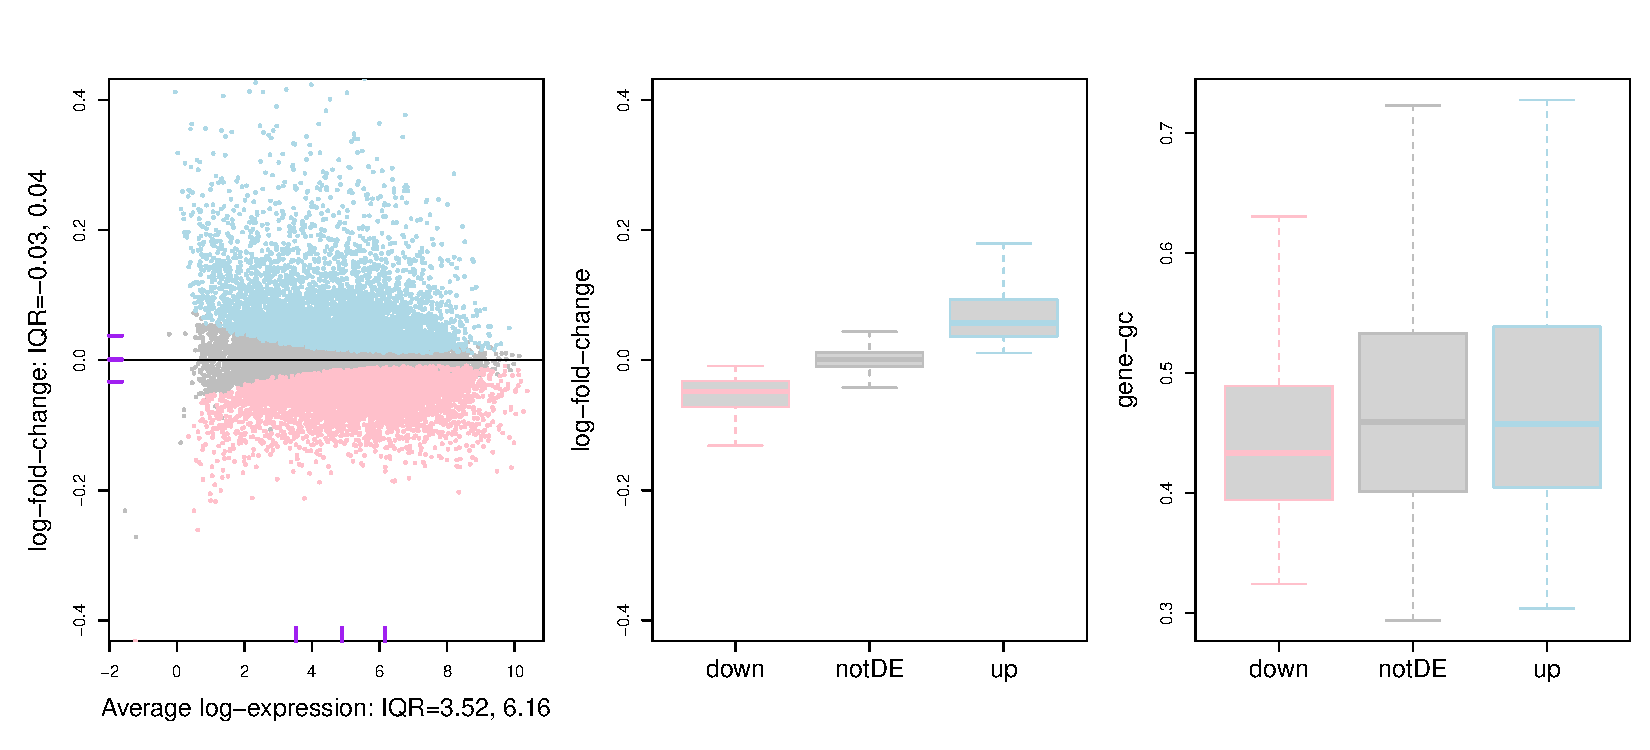
\includegraphics{Static/figures/mdPlotEfit-1.pdf}
\caption{\label{fig:mdPlotEfit}HCC vs Control - Genes Identified at FDR = 0,05}
\end{figure}

\begin{Shaded}
\begin{Highlighting}[]
 \CommentTok{\#mtext(side=3, outer=T, cex=1.25, "Genes identified at adjusted p{-}value=0.05")}
\end{Highlighting}
\end{Shaded}

\begin{Shaded}
\begin{Highlighting}[]
\NormalTok{featureCountsAF\_logFC\_sum <{-}}\StringTok{ }\KeywordTok{sapply}\NormalTok{(}
 \KeywordTok{split}\NormalTok{(}
\NormalTok{ filteredCountsAF\_voom\_efit}\OperatorTok{$}\NormalTok{coefficients[, }\StringTok{\textquotesingle{}HCCvsControl\textquotesingle{}}\NormalTok{],}
\NormalTok{ filteredCountsAF\_voom\_efit\_dt[,}\StringTok{\textquotesingle{}HCCvsControl\textquotesingle{}}\NormalTok{]),}
\NormalTok{ quantile, }\DataTypeTok{prob =}\NormalTok{ (}\DecValTok{1}\OperatorTok{:}\DecValTok{3}\NormalTok{) }\OperatorTok{/}\StringTok{ }\DecValTok{4}\NormalTok{)}

\KeywordTok{colnames}\NormalTok{(featureCountsAF\_logFC\_sum) <{-}}\StringTok{ }\KeywordTok{as.character}\NormalTok{(}\KeywordTok{factor}\NormalTok{(}
 \KeywordTok{colnames}\NormalTok{(featureCountsAF\_logFC\_sum), }
 \DataTypeTok{levels=}\KeywordTok{c}\NormalTok{(}\StringTok{"{-}1"}\NormalTok{, }\StringTok{"0"}\NormalTok{, }\StringTok{"1"}\NormalTok{),}
 \DataTypeTok{labels=}\KeywordTok{c}\NormalTok{(}\StringTok{\textquotesingle{}down\textquotesingle{}}\NormalTok{, }\StringTok{\textquotesingle{}notDE\textquotesingle{}}\NormalTok{, }\StringTok{\textquotesingle{}up\textquotesingle{}}\NormalTok{)}
\NormalTok{))}


\NormalTok{knitr}\OperatorTok{::}\KeywordTok{kable}\NormalTok{(featureCountsAF\_logFC\_sum,}
  \DataTypeTok{digits =} \DecValTok{2}\NormalTok{,}
  \DataTypeTok{caption =} \StringTok{"log FC quartiles by gene identification"}\NormalTok{) }\OperatorTok{\%>\%}
\StringTok{  }\NormalTok{kableExtra}\OperatorTok{::}\KeywordTok{kable\_styling}\NormalTok{(}\DataTypeTok{full\_width =}\NormalTok{ F)}
\end{Highlighting}
\end{Shaded}

\begin{table}

\caption{\label{tab:quantlogFC}log FC quartiles by gene identification}
\centering
\begin{tabular}[t]{l|r|r|r}
\hline
  & down & notDE & up\\
\hline
25\% & -0.07 & -0.01 & 0.04\\
\hline
50\% & -0.05 & 0.00 & 0.06\\
\hline
75\% & -0.03 & 0.01 & 0.09\\
\hline
\end{tabular}
\end{table}

While many genes are identified, the effect sizes are quite small,
which results in a low signal-to-noise ratio context. See
Section \ref{snr-regime} below.

The log-fold-change distribution for up-represented genes is long-tailed,
with many high log fold-change values.
By contrast, log-fold-change distribution for down-represented genes
closer to symmetric and has few genes with low log fold-change values.
We will see how this affects the results of identifying genes with
an effect size requirement.

The GC content of down regulated genes tends to be slightly lower than the
rest of the genes. A statistical test would find that the difference
between the mean of the down regulated gene population is singificantly different
than the mean of the other gene population even though the difference is
quite small
(\(-0.028\)).

These asymmetries are minor, but it would still be good to establish that
they relfect biology rather than processing artifacts.

\hypertarget{de-genes-at-10-fold-change}{%
\subsection*{DE genes at 10\% fold change}\label{de-genes-at-10-fold-change}}
\addcontentsline{toc}{subsection}{DE genes at 10\% fold change}

For a stricter definition on significance, one may require log-fold-changes
(log-FCs) to be above a minimum value. The treat method
(McCarthy and Smyth 2009 {[}\protect\hyperlink{ref-McCarthy:2009aa}{23}{]}) can be used to calculate p-values
from empirical Bayes moderated t-statistics with a minimum log-FC requirement.
The number of differentially expressed genes are greatly reduced if we
impose a minimal fold-change requirement of 10\%.

\begin{Shaded}
\begin{Highlighting}[]
\NormalTok{filteredCountsAF\_voom\_tfit <{-}}\StringTok{ }\NormalTok{limma}\OperatorTok{::}\KeywordTok{treat}\NormalTok{(filteredCountsAF\_voom\_fit, }\DataTypeTok{lfc=}\KeywordTok{log2}\NormalTok{(}\FloatTok{1.10}\NormalTok{))}
\NormalTok{filteredCountsAF\_voom\_tfit\_dt <{-}}\StringTok{ }\NormalTok{limma}\OperatorTok{::}\KeywordTok{decideTests}\NormalTok{(filteredCountsAF\_voom\_tfit)}

\KeywordTok{cat}\NormalTok{(}\StringTok{"10\% FC Gene Identification Summary {-} voom, adjust.method = BH, p.value = 0.05:}\CharTok{\textbackslash{}n}\StringTok{"}\NormalTok{)}
\end{Highlighting}
\end{Shaded}

\begin{verbatim}
## 10% FC Gene Identification Summary - voom, adjust.method = BH, p.value = 0.05:
\end{verbatim}

\begin{Shaded}
\begin{Highlighting}[]
\KeywordTok{summary}\NormalTok{(filteredCountsAF\_voom\_tfit\_dt)}
\end{Highlighting}
\end{Shaded}

\begin{verbatim}
##        HCCvsControl
## Down              3
## NotSig        15550
## Up              199
\end{verbatim}

\begin{Shaded}
\begin{Highlighting}[]
\CommentTok{\# log{-}fold{-}change vs ave{-}expr}
\NormalTok{limma}\OperatorTok{::}\KeywordTok{plotMD}\NormalTok{(filteredCountsAF\_voom\_efit,}
 \DataTypeTok{ylim =} \KeywordTok{c}\NormalTok{(}\OperatorTok{{-}}\FloatTok{0.5}\NormalTok{, }\FloatTok{0.5}\NormalTok{),}
 \DataTypeTok{column=}\StringTok{\textquotesingle{}HCCvsControl\textquotesingle{}}\NormalTok{,}
 \DataTypeTok{status=}\NormalTok{filteredCountsAF\_voom\_tfit\_dt[,}\StringTok{\textquotesingle{}HCCvsControl\textquotesingle{}}\NormalTok{],}
 \DataTypeTok{hl.pch =} \DecValTok{16}\NormalTok{, }\DataTypeTok{hl.col =} \KeywordTok{c}\NormalTok{(}\StringTok{"blue"}\NormalTok{, }\StringTok{"red"}\NormalTok{), }\DataTypeTok{hl.cex =} \FloatTok{.7}\NormalTok{,}
 \DataTypeTok{bg.pch =} \DecValTok{16}\NormalTok{, }\DataTypeTok{bg.col =} \StringTok{"grey"}\NormalTok{, }\DataTypeTok{bg.cex =} \FloatTok{0.5}\NormalTok{,}
 \DataTypeTok{main =} \StringTok{\textquotesingle{}\textquotesingle{}}\NormalTok{,}
 \DataTypeTok{xlab =} \KeywordTok{paste0}\NormalTok{(}
    \StringTok{"Average log{-}expression: IQR="}\NormalTok{,}
    \KeywordTok{paste}\NormalTok{(}\KeywordTok{round}\NormalTok{(}\KeywordTok{quantile}\NormalTok{(filteredCountsAF\_voom\_efit}\OperatorTok{$}\NormalTok{Amean, }\DataTypeTok{prob =} \KeywordTok{c}\NormalTok{(}\DecValTok{1}\NormalTok{, }\DecValTok{3}\NormalTok{) }\OperatorTok{/}\StringTok{ }\DecValTok{4}\NormalTok{), }\DecValTok{2}\NormalTok{),}
      \DataTypeTok{collapse =} \StringTok{", "}
\NormalTok{    )}
\NormalTok{  ),}
  \DataTypeTok{ylab =} \KeywordTok{paste0}\NormalTok{(}
    \StringTok{"log{-}fold{-}change: IQR="}\NormalTok{,}
    \KeywordTok{paste}\NormalTok{(}\KeywordTok{round}\NormalTok{(}\KeywordTok{quantile}\NormalTok{(filteredCountsAF\_voom\_efit}\OperatorTok{$}\NormalTok{coefficients[, }\StringTok{\textquotesingle{}HCCvsControl\textquotesingle{}}\NormalTok{], }\DataTypeTok{prob =} \KeywordTok{c}\NormalTok{(}\DecValTok{1}\NormalTok{, }\DecValTok{3}\NormalTok{) }\OperatorTok{/}\StringTok{ }\DecValTok{4}\NormalTok{), }\DecValTok{2}\NormalTok{),}
      \DataTypeTok{collapse =} \StringTok{", "}
\NormalTok{    )}
\NormalTok{  ),}
  \DataTypeTok{legend =}\NormalTok{ F}
\NormalTok{)}
\KeywordTok{abline}\NormalTok{(}\DataTypeTok{h =} \DecValTok{0}\NormalTok{, }\DataTypeTok{col =} \StringTok{"black"}\NormalTok{)}
\KeywordTok{rug}\NormalTok{(}\KeywordTok{quantile}\NormalTok{(filteredCountsAF\_voom\_efit}\OperatorTok{$}\NormalTok{coefficients[, }\StringTok{\textquotesingle{}HCCvsControl\textquotesingle{}}\NormalTok{], }\DataTypeTok{prob =} \KeywordTok{c}\NormalTok{(}\DecValTok{1}\NormalTok{, }\DecValTok{2}\NormalTok{, }\DecValTok{3}\NormalTok{) }\OperatorTok{/}\StringTok{ }\DecValTok{4}\NormalTok{),}
  \DataTypeTok{col =} \StringTok{"purple"}\NormalTok{,}
  \DataTypeTok{ticksize =} \FloatTok{.03}\NormalTok{, }\DataTypeTok{side =} \DecValTok{2}\NormalTok{, }\DataTypeTok{lwd =} \DecValTok{2}
\NormalTok{)}
\KeywordTok{rug}\NormalTok{(}\KeywordTok{quantile}\NormalTok{(filteredCountsAF\_voom\_efit}\OperatorTok{$}\NormalTok{Amean, }\DataTypeTok{prob =} \KeywordTok{c}\NormalTok{(}\DecValTok{1}\NormalTok{, }\DecValTok{2}\NormalTok{, }\DecValTok{3}\NormalTok{) }\OperatorTok{/}\StringTok{ }\DecValTok{4}\NormalTok{),}
  \DataTypeTok{col =} \StringTok{"purple"}\NormalTok{,}
  \DataTypeTok{ticksize =} \FloatTok{.03}\NormalTok{, }\DataTypeTok{side =} \DecValTok{1}\NormalTok{, }\DataTypeTok{lwd =} \DecValTok{2}
\NormalTok{)}
\end{Highlighting}
\end{Shaded}

\begin{figure}
\centering
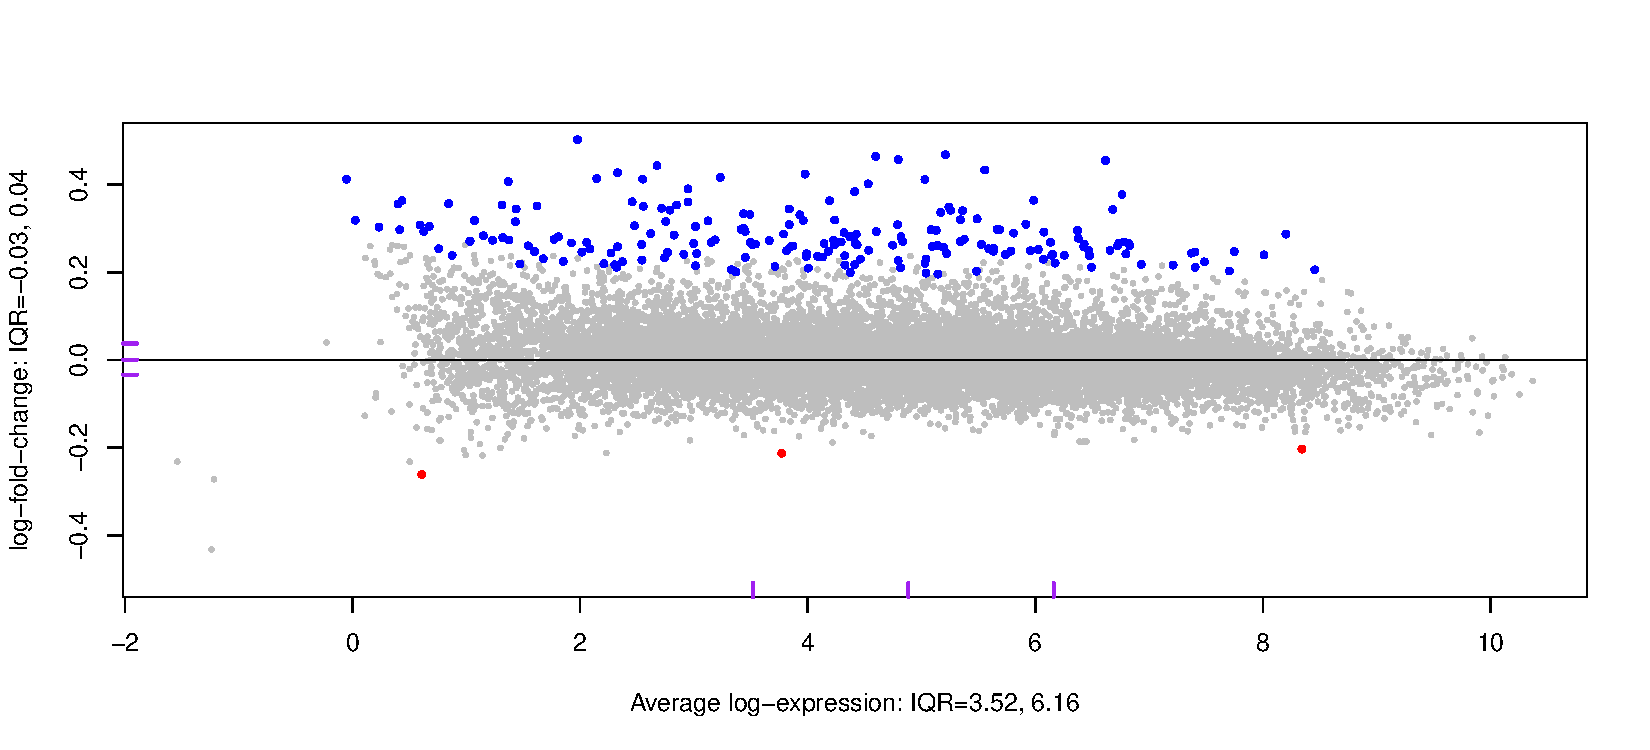
\includegraphics{Static/figures/mdPlotTfit-1.pdf}
\caption{\label{fig:mdPlotTfit}HCC vs Control - Identified Genes at FDR = 0,05 and logFC \textgreater{} 10\%}
\end{figure}

As noted above, the log-fold-change distribution for the up-represented genes
is long-tailes in comparison to log-fold-change distribution for the down-represented genes.
As a result fewer down-represented than up-regulated genes are identified when a
minimum log-FC requirement is imposed.

\hypertarget{snr-regime}{%
\section{Signal-to-noise ratio regime}\label{snr-regime}}

In Hastie et al.~(2017) {[}\protect\hyperlink{ref-Hastie:2017aa}{7}{]}) results from \texttt{lasso} fits are
compared with \texttt{best\ subset} and \texttt{forward\ selection} fits and it is argued
that while \texttt{best\ subset} is optimal for high signal-to-noise regimes,
the lasso gains some competitive advantage when the prevailing signal-to-noise
ratio of the dataset is lowered.

We can extract sigma and signal from the fit objects to get SNR values for each gene
to see in what SNR regime the 5hmC gene body data are.

\begin{Shaded}
\begin{Highlighting}[]
\NormalTok{lib.size <{-}}\StringTok{ }\KeywordTok{colSums}\NormalTok{(AF\_dgel}\OperatorTok{$}\NormalTok{counts)}

\NormalTok{fit <{-}}\StringTok{ }\NormalTok{filteredCountsAF\_voom\_efit}
\NormalTok{sx <{-}}\StringTok{ }\NormalTok{fit}\OperatorTok{$}\NormalTok{Amean }\OperatorTok{+}\StringTok{ }\KeywordTok{mean}\NormalTok{(}\KeywordTok{log2}\NormalTok{(lib.size }\OperatorTok{+}\StringTok{ }\DecValTok{1}\NormalTok{)) }\OperatorTok{{-}}\StringTok{ }\KeywordTok{log2}\NormalTok{(}\FloatTok{1e+06}\NormalTok{)}
\NormalTok{sy <{-}}\StringTok{ }\KeywordTok{sqrt}\NormalTok{(fit}\OperatorTok{$}\NormalTok{sigma)}

\NormalTok{CV <{-}}\StringTok{ }\NormalTok{sy}\OperatorTok{/}\NormalTok{sx    }
\end{Highlighting}
\end{Shaded}

\begin{Shaded}
\begin{Highlighting}[]
\NormalTok{Effect <{-}}\StringTok{ }\KeywordTok{abs}\NormalTok{(filteredCountsAF\_voom\_efit}\OperatorTok{$}\NormalTok{coefficients[,}\StringTok{\textquotesingle{}HCCvsControl\textquotesingle{}}\NormalTok{])}
\NormalTok{Noise <{-}}\StringTok{ }\NormalTok{filteredCountsAF\_voom\_efit}\OperatorTok{$}\NormalTok{sigma}
\NormalTok{SNR <{-}}\StringTok{ }\NormalTok{Effect}\OperatorTok{/}\NormalTok{Noise}

\KeywordTok{plot}\NormalTok{(spatstat}\OperatorTok{::}\KeywordTok{CDF}\NormalTok{(}\KeywordTok{density}\NormalTok{(SNR)),}
  \DataTypeTok{col =} \DecValTok{1}\NormalTok{, }\DataTypeTok{lwd =} \DecValTok{2}\NormalTok{, }\DataTypeTok{ylab =} \StringTok{"Prob(SNR<x)"}\NormalTok{,}
  \DataTypeTok{xlim =} \KeywordTok{c}\NormalTok{(}\DecValTok{0}\NormalTok{, }\FloatTok{0.2}\NormalTok{)}
\NormalTok{)}

\NormalTok{SNR\_quant <{-}}\StringTok{ }\KeywordTok{quantile}\NormalTok{(SNR, }\DataTypeTok{prob=}\KeywordTok{c}\NormalTok{((}\DecValTok{1}\OperatorTok{:}\DecValTok{3}\NormalTok{)}\OperatorTok{/}\DecValTok{4}\NormalTok{,.}\DecValTok{9}\NormalTok{))}
\KeywordTok{rug}\NormalTok{(SNR\_quant,}
    \DataTypeTok{lwd =} \DecValTok{2}\NormalTok{, }\DataTypeTok{ticksize =} \FloatTok{0.05}\NormalTok{, }\DataTypeTok{col =} \DecValTok{1}
\NormalTok{  )}
\end{Highlighting}
\end{Shaded}

\begin{figure}
\centering
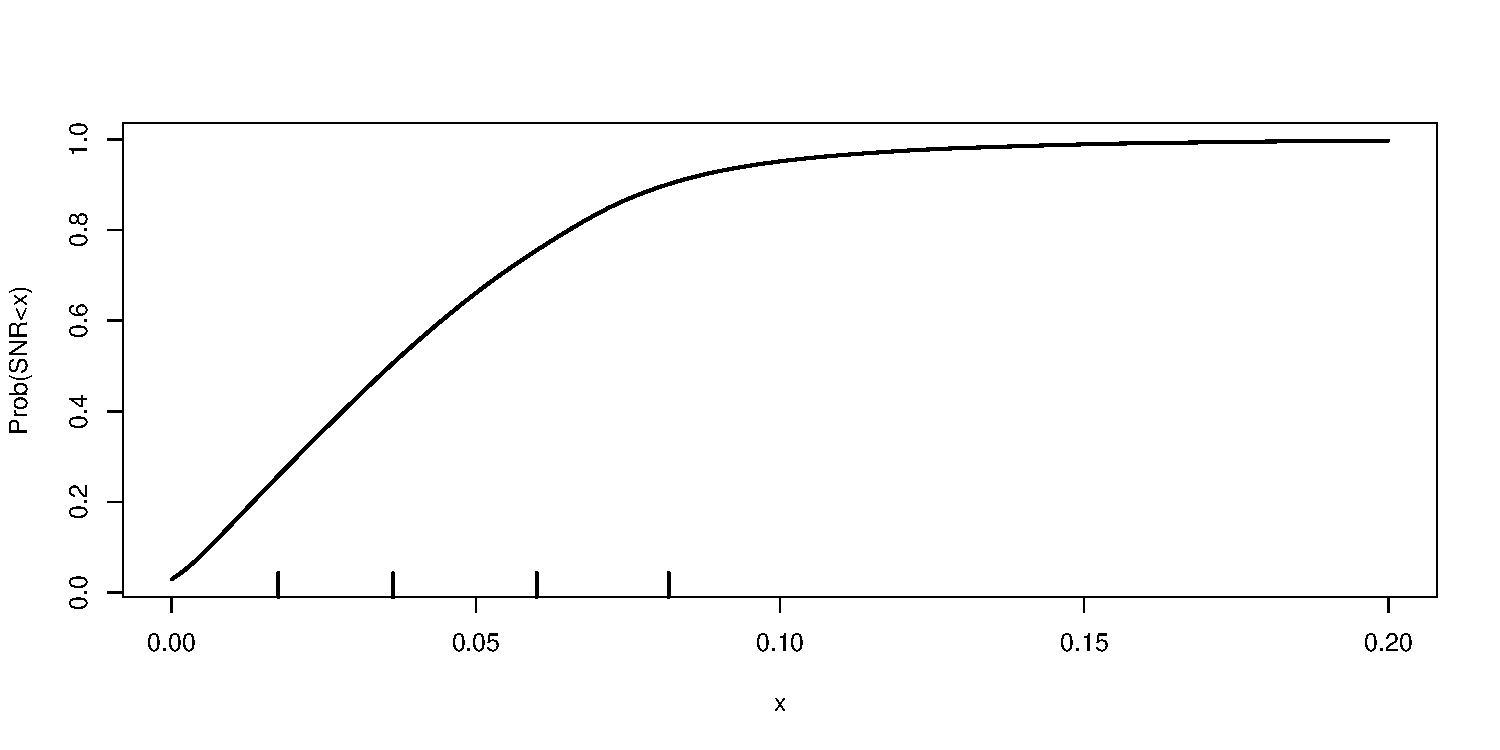
\includegraphics{Static/figures/plotSNR-1.pdf}
\caption{\label{fig:plotSNR}Cumulative Distribution of SNR - rug = 25, 50, 75 and 90th percentile}
\end{figure}

\begin{Shaded}
\begin{Highlighting}[]
\NormalTok{knitr}\OperatorTok{::}\KeywordTok{kable}\NormalTok{(}\KeywordTok{t}\NormalTok{(SNR\_quant),}
  \DataTypeTok{digits =} \DecValTok{3}\NormalTok{,}
  \DataTypeTok{caption =} \KeywordTok{paste}\NormalTok{(}
    \StringTok{"SNR Quantiles"}\NormalTok{) }
\NormalTok{) }\OperatorTok{\%>\%}\StringTok{ }\NormalTok{kableExtra}\OperatorTok{::}\KeywordTok{kable\_styling}\NormalTok{(}\DataTypeTok{full\_width =}\NormalTok{ F)}
\end{Highlighting}
\end{Shaded}

\begin{table}

\caption{\label{tab:plotSNR}SNR Quantiles}
\centering
\begin{tabular}[t]{r|r|r|r}
\hline
25\% & 50\% & 75\% & 90\%\\
\hline
0.018 & 0.036 & 0.06 & 0.082\\
\hline
\end{tabular}
\end{table}

These SNR values are in the range where the lasso and relaxed lasso gain some advantage over
best subset and forward selection fits (see Hastie et al.~(2017) {[}\protect\hyperlink{ref-Hastie:2017aa}{7}{]}).

\hypertarget{explore-sparsity}{%
\chapter{The bet on sparsity}\label{explore-sparsity}}

In this section we explore various fits that can be computed
and analyzed with tools provided in the \texttt{glmnet} package.
Refer to the \href{https://web.stanford.edu/~hastie/glmnet/glmnet_alpha.html}{Glmnet Vignette}
for a quick reference guide. We focus our analyses on lasso fits
which tend to favor sparse models.

\hypertarget{cross-validation-analysis-setup}{%
\section{Cross-validation analysis setup}\label{cross-validation-analysis-setup}}

\begin{Shaded}
\begin{Highlighting}[]
\NormalTok{K\_FOLD <{-}}\StringTok{ }\DecValTok{10}
\NormalTok{trainP <{-}}\StringTok{ }\FloatTok{0.8}
\end{Highlighting}
\end{Shaded}

First we divide the analysis dataset into \texttt{train} and \texttt{test} in a \(4\):1 ratio.

\begin{Shaded}
\begin{Highlighting}[]
\KeywordTok{set.seed}\NormalTok{(}\DecValTok{1}\NormalTok{)}
\NormalTok{train\_sampID\_vec <{-}}\StringTok{ }\KeywordTok{with}\NormalTok{(AF\_dgel}\OperatorTok{$}\NormalTok{samples,}
\NormalTok{AF\_dgel}\OperatorTok{$}\NormalTok{samples}\OperatorTok{$}\NormalTok{sampID[caret}\OperatorTok{::}\KeywordTok{createDataPartition}\NormalTok{(}\DataTypeTok{y=}\NormalTok{group, }\DataTypeTok{p=}\NormalTok{trainP, }\DataTypeTok{list=}\NormalTok{F)]}
\NormalTok{)}

\NormalTok{test\_sampID\_vec <{-}}\StringTok{ }\KeywordTok{with}\NormalTok{(AF\_dgel}\OperatorTok{$}\NormalTok{samples,}
\KeywordTok{setdiff}\NormalTok{(sampID, train\_sampID\_vec)}
\NormalTok{)}

\NormalTok{train\_group\_vec <{-}}\StringTok{ }\NormalTok{AF\_dgel}\OperatorTok{$}\NormalTok{samples[train\_sampID\_vec, }\StringTok{\textquotesingle{}group\textquotesingle{}}\NormalTok{]}
\KeywordTok{names}\NormalTok{(train\_group\_vec) <{-}}\StringTok{ }\NormalTok{AF\_dgel}\OperatorTok{$}\NormalTok{samples[train\_sampID\_vec, }\StringTok{\textquotesingle{}sampID\textquotesingle{}}\NormalTok{]}

\NormalTok{test\_group\_vec <{-}}\StringTok{ }\NormalTok{AF\_dgel}\OperatorTok{$}\NormalTok{samples[test\_sampID\_vec, }\StringTok{\textquotesingle{}group\textquotesingle{}}\NormalTok{]}
\KeywordTok{names}\NormalTok{(test\_group\_vec) <{-}}\StringTok{ }\NormalTok{AF\_dgel}\OperatorTok{$}\NormalTok{samples[test\_sampID\_vec, }\StringTok{\textquotesingle{}sampID\textquotesingle{}}\NormalTok{]}

\NormalTok{knitr}\OperatorTok{::}\KeywordTok{kable}\NormalTok{(}\KeywordTok{table}\NormalTok{(train\_group\_vec),}
  \DataTypeTok{caption=}\StringTok{"Train set"}\NormalTok{) }\OperatorTok{\%>\%}
\StringTok{   }\NormalTok{kableExtra}\OperatorTok{::}\KeywordTok{kable\_styling}\NormalTok{(}\DataTypeTok{full\_width =}\NormalTok{ F)}
\end{Highlighting}
\end{Shaded}

\begin{table}

\caption{\label{tab:getTrainVal}Train set}
\centering
\begin{tabular}[t]{l|r}
\hline
train\_group\_vec & Freq\\
\hline
Control & 623\\
\hline
HCC & 444\\
\hline
\end{tabular}
\end{table}

\begin{Shaded}
\begin{Highlighting}[]
\NormalTok{knitr}\OperatorTok{::}\KeywordTok{kable}\NormalTok{(}\KeywordTok{table}\NormalTok{(test\_group\_vec),}
  \DataTypeTok{caption=}\StringTok{"Test set"}\NormalTok{) }\OperatorTok{\%>\%}
\StringTok{   }\NormalTok{kableExtra}\OperatorTok{::}\KeywordTok{kable\_styling}\NormalTok{(}\DataTypeTok{full\_width =}\NormalTok{ F)}
\end{Highlighting}
\end{Shaded}

\begin{table}

\caption{\label{tab:getTrainVal}Test set}
\centering
\begin{tabular}[t]{l|r}
\hline
test\_group\_vec & Freq\\
\hline
Control & 155\\
\hline
HCC & 111\\
\hline
\end{tabular}
\end{table}

\begin{Shaded}
\begin{Highlighting}[]
\NormalTok{train\_lcpm\_mtx <{-}}\StringTok{ }\KeywordTok{t}\NormalTok{(lcpm\_mtx[,train\_sampID\_vec])}
\NormalTok{test\_lcpm\_mtx <{-}}\StringTok{ }\KeywordTok{t}\NormalTok{(lcpm\_mtx[,test\_sampID\_vec])}
\end{Highlighting}
\end{Shaded}

We explore some glmnet fits and the ``bet on sparsity''.
We consider three models, specified by the value of the
\textbf{alpha} parameter in the elastic net parametrization:\\
- lasso: \(\alpha = 1.0\) - sparse models\\
- ridge \(\alpha = 0\) - shrunken coefficients models\\
- elastic net: \(\alpha = 0.5\) - semi sparse model\\

Some questions of interest include:

\begin{itemize}
\tightlist
\item
  How sparse are models enabling good 5hmC classification of Early HCC vs Control samples?
\end{itemize}

\begin{itemize}
\item
  Does the shrunken relaxed lasso (aka the blended mix) improve performance in this case?
\item
  Is the degree of sparsity, or the size of the model, a stable feature of the problem and data set?
\end{itemize}

In this analysis, we will only evaluate models in terms of
model sparsity, stability and performance. We leave the question
of significance testing of hypotheses about model parameters
completely out. See Lockhart et al.~(2014) {[}\protect\hyperlink{ref-Lockhart:2014aa}{24}{]}
and Wassermam (2014) {[}\protect\hyperlink{ref-Wasserman:2014aa}{25}{]} for a discussion of this topic.

In this section we look at the relative performance and sparsity of the models
considered. The effect of the size of the sample set on the level and
stability of performance will be investigated in the next section.

\begin{center}\rule{0.5\linewidth}{0.5pt}\end{center}

First we create folds for \(10\)-fold cross-validation of models fitted to
training data. We'll use caret::createFolds to assign samples
to folds while keeping the outcome ratios constant across folds.

\begin{Shaded}
\begin{Highlighting}[]
\CommentTok{\# This is too variable, both in terms of fold size And composition}
\CommentTok{\#foldid\_vec <{-} sample(1:10, size=length(train\_group\_vec), replace=T)}

\KeywordTok{set.seed}\NormalTok{(}\DecValTok{1}\NormalTok{)}
\NormalTok{train\_foldid\_vec <{-}}\StringTok{ }\NormalTok{caret}\OperatorTok{::}\KeywordTok{createFolds}\NormalTok{(}
 \KeywordTok{factor}\NormalTok{(train\_group\_vec), }
 \DataTypeTok{k=}\NormalTok{K\_FOLD,}
 \DataTypeTok{list=}\NormalTok{F)}

\CommentTok{\# train\_foldid\_vec contains the left{-}out IDs }
\CommentTok{\# the rest are kept}
\NormalTok{fold\_out\_tbl <{-}}\StringTok{ }\KeywordTok{sapply}\NormalTok{(}\KeywordTok{split}\NormalTok{(train\_group\_vec, train\_foldid\_vec),}
\NormalTok{  table)}
\KeywordTok{rownames}\NormalTok{(fold\_out\_tbl) <{-}}\StringTok{ }\KeywordTok{paste}\NormalTok{(}\KeywordTok{rownames}\NormalTok{(fold\_out\_tbl), }\StringTok{\textquotesingle{}{-} Out\textquotesingle{}}\NormalTok{) }

\NormalTok{fold\_in\_tbl <{-}}\StringTok{ }\KeywordTok{do.call}\NormalTok{(}\StringTok{\textquotesingle{}cbind\textquotesingle{}}\NormalTok{, }\KeywordTok{lapply}\NormalTok{(}\KeywordTok{sort}\NormalTok{(}\KeywordTok{unique}\NormalTok{(train\_foldid\_vec)),}
  \ControlFlowTok{function}\NormalTok{(FOLD) }\KeywordTok{table}\NormalTok{(train\_group\_vec[train\_foldid\_vec }\OperatorTok{!=}\StringTok{ }\NormalTok{FOLD])))}
\KeywordTok{rownames}\NormalTok{(fold\_in\_tbl) <{-}}\StringTok{ }\KeywordTok{paste}\NormalTok{(}\KeywordTok{rownames}\NormalTok{(fold\_in\_tbl), }\StringTok{\textquotesingle{}{-} In\textquotesingle{}}\NormalTok{) }
\KeywordTok{colnames}\NormalTok{(fold\_in\_tbl) <{-}}\StringTok{ }\KeywordTok{as.character}\NormalTok{(}\KeywordTok{sort}\NormalTok{(}\KeywordTok{unique}\NormalTok{(train\_foldid\_vec)))}


\NormalTok{knitr}\OperatorTok{::}\KeywordTok{kable}\NormalTok{(}\KeywordTok{rbind}\NormalTok{(fold\_in\_tbl, fold\_out\_tbl[,}\KeywordTok{colnames}\NormalTok{(fold\_in\_tbl)]),}
  \DataTypeTok{caption=}\StringTok{"training samples fold composition"}\NormalTok{) }\OperatorTok{\%>\%}
\StringTok{   }\NormalTok{kableExtra}\OperatorTok{::}\KeywordTok{kable\_styling}\NormalTok{(}\DataTypeTok{full\_width =}\NormalTok{ F)}
\end{Highlighting}
\end{Shaded}

\begin{table}

\caption{\label{tab:getTrainFolds}training samples fold composition}
\centering
\begin{tabular}[t]{l|r|r|r|r|r|r|r|r|r|r}
\hline
  & 1 & 2 & 3 & 4 & 5 & 6 & 7 & 8 & 9 & 10\\
\hline
Control - In & 561 & 561 & 561 & 560 & 561 & 561 & 560 & 561 & 560 & 561\\
\hline
HCC - In & 399 & 400 & 400 & 399 & 400 & 399 & 400 & 399 & 400 & 400\\
\hline
Control - Out & 62 & 62 & 62 & 63 & 62 & 62 & 63 & 62 & 63 & 62\\
\hline
HCC - Out & 45 & 44 & 44 & 45 & 44 & 45 & 44 & 45 & 44 & 44\\
\hline
\end{tabular}
\end{table}

Note that the folds identify samples that are left-out of the training
data for each fold fit.

\hypertarget{fit-and-compare-models}{%
\section{Fit and compare models}\label{fit-and-compare-models}}

\texttt{glmnet} provides cross-validation methods to pick the parameter \textbf{lambda} which
controls to size of the penalty function. The ``one standard error rule''
produces a model with fewer predictors then the minimum cv error model.
On the training data, this usually results in increased MSE and more
biased parameter estimates
(see Engebretsen et al.~(2019) {[}\protect\hyperlink{ref-Engebretsen:2019aa}{26}{]} for example).
The question of iterest though is the performance on unseen data; not on the training data.
In the analysis below, we compare the cv error rates with out-of-fold and
test set error rates. The results show that out-of-fold error rates computed from
the training data are good indicators of test set error rates, and that
the one standard error rule models do as well as the minimim cv error models
for the lasso, which has the best overall performance.

\hypertarget{logistic-regression-in-glmnet}{%
\subsection{\texorpdfstring{Logistic regression in \texttt{glmnet}}{Logistic regression in glmnet}}\label{logistic-regression-in-glmnet}}

\texttt{glmnet} provides functionality to extract various predicted of fitted values
from calibrated models. Note that some folks make a distinction between
\textbf{fitted} or \textbf{estimated} values for sample points in the training data
versus \textbf{predicted} values for sample points that
are not in the training dataset. \texttt{glmnet} makes no such distinction and the
\texttt{predict} function is used to produce both fitted as well as predicted values.
When predict is invoked to make predictions for design points that are part
of the training dataset, what is returned are fitted values.
When predict is invoked to make predictions for design points that are not part
of the training dataset, what is returned are predicted values.

For logistic regressions, which is the model fitted in a regularized fashion
when models are fitted by glmnet with the parameter \texttt{family=\textquotesingle{}binomial\textquotesingle{}}, three
fitted or predicted values can be extracted at a given design point.
Suppose our response variable Y is either 0 or 1 (Control or HCC in our case).
These are specified by the \texttt{type} parameter. \texttt{type=\textquotesingle{}resp\textquotesingle{}} returns
the fitted or predicted probability of \(Y=1\). \texttt{type=\textquotesingle{}class\textquotesingle{}} returns the fitted or
predicted class for the design point, which is simply dichotomizing the
response: class = 1 if the fitted or predicted probability is greater than 0.5
(check to make sure class is no the Bayes estimate). \texttt{type=\textquotesingle{}link\textquotesingle{}} returns
the fitted or predicted value of the linear predictor \(\beta'x\). The relationship
between the linear predictor and the response can be derided from the
logistic regression model:

\[P(Y=1|x,\beta) = g^{-1}(\beta'x) = h(\beta'x) = \frac{e^{\beta'x}}{1+e^{\beta'x}}\]

where \(g\) is the link function, \(g^{-1}\) the mean function.
The link function is given by:

\[g(y) = h^{-1}(y) = ln(\frac{y}{1-y})\]

This link function is called the \emph{logit} function, and its inverse the \emph{logistic}
function.

\begin{Shaded}
\begin{Highlighting}[]
\NormalTok{logistic\_f <{-}}\StringTok{ }\ControlFlowTok{function}\NormalTok{(x) }\KeywordTok{exp}\NormalTok{(x)}\OperatorTok{/}\NormalTok{(}\DecValTok{1}\OperatorTok{+}\KeywordTok{exp}\NormalTok{(x))}
\end{Highlighting}
\end{Shaded}

We should also point out that the cv error rates quoted in various \texttt{glmnet} summaries
are computed from out-of-fold predictions. In other words,
we cannot recover the \texttt{cvm} component of a glmnet fit object by comparing
class predictions extracted by invoking \texttt{predict()} with paramters \texttt{newx\ =\ train\_data}
and \texttt{type\ =\ \textquotesingle{}class\textquotesingle{}} to the true class labels.

\texttt{glmnet} fitting functions have a
parameter, \emph{keep}, which instructs the fitting function to keep the
\texttt{out-of-fold}, or \texttt{prevalidated}, predictions as part of the returned object. The
\texttt{out-of-fold} predictions are predicted values for the samples in the
left-out folds, pooled across all cv folds. For each hyper-parameter
specification, we get one full set of \texttt{out-of-fold} predictions for
the training set samples. Performance assessments based on these
values are usually more generalizable. The \texttt{cvm} component of glmnet fitted
objects are derived from these \texttt{out-of-fold} predictions.
See Hofling and Tibshirani (2008) {[}\protect\hyperlink{ref-Hofling:2008aa}{27}{]}
for a description of the use of pre-validation in model assessment.

\begin{Shaded}
\begin{Highlighting}[]
\NormalTok{start\_time <{-}}\StringTok{  }\KeywordTok{proc.time}\NormalTok{()}

\NormalTok{cv\_lasso <{-}}\StringTok{ }\NormalTok{glmnet}\OperatorTok{::}\KeywordTok{cv.glmnet}\NormalTok{(}
 \DataTypeTok{x=}\NormalTok{train\_lcpm\_mtx,}
 \DataTypeTok{y=}\NormalTok{train\_group\_vec,}
 \DataTypeTok{foldid=}\NormalTok{train\_foldid\_vec,}
 \DataTypeTok{alpha=}\DecValTok{1}\NormalTok{,}
 \DataTypeTok{family=}\StringTok{\textquotesingle{}binomial\textquotesingle{}}\NormalTok{, }
 \DataTypeTok{type.measure =} \StringTok{"class"}\NormalTok{,}
 \DataTypeTok{keep=}\NormalTok{T,}
 \DataTypeTok{nlambda=}\DecValTok{30}
\NormalTok{)}

\KeywordTok{message}\NormalTok{(}\StringTok{"lasso time: "}\NormalTok{, }\KeywordTok{round}\NormalTok{((}\KeywordTok{proc.time}\NormalTok{() }\OperatorTok{{-}}\StringTok{ }\NormalTok{start\_time)[}\DecValTok{3}\NormalTok{],}\DecValTok{2}\NormalTok{),}\StringTok{"s"}\NormalTok{)}
\end{Highlighting}
\end{Shaded}

\begin{verbatim}
## lasso time: 12.96s
\end{verbatim}

\begin{Shaded}
\begin{Highlighting}[]
\NormalTok{start\_time <{-}}\StringTok{  }\KeywordTok{proc.time}\NormalTok{()}

\NormalTok{cv\_ridge <{-}}\StringTok{ }\NormalTok{glmnet}\OperatorTok{::}\KeywordTok{cv.glmnet}\NormalTok{(}
 \DataTypeTok{x=}\NormalTok{train\_lcpm\_mtx,}
 \DataTypeTok{y=}\NormalTok{train\_group\_vec,}
 \DataTypeTok{foldid=}\NormalTok{train\_foldid\_vec,}
 \DataTypeTok{alpha=}\DecValTok{0}\NormalTok{,}
 \DataTypeTok{family=}\StringTok{\textquotesingle{}binomial\textquotesingle{}}\NormalTok{, }
 \DataTypeTok{type.measure =} \StringTok{"class"}\NormalTok{,}
 \DataTypeTok{keep=}\NormalTok{T,}
 \DataTypeTok{nlambda=}\DecValTok{30}
\NormalTok{)}

\KeywordTok{message}\NormalTok{(}\StringTok{"ridge time: "}\NormalTok{, }\KeywordTok{round}\NormalTok{((}\KeywordTok{proc.time}\NormalTok{() }\OperatorTok{{-}}\StringTok{ }\NormalTok{start\_time)[}\DecValTok{3}\NormalTok{],}\DecValTok{2}\NormalTok{),}\StringTok{"s"}\NormalTok{)}
\end{Highlighting}
\end{Shaded}

\begin{verbatim}
## ridge time: 105.8s
\end{verbatim}

\begin{Shaded}
\begin{Highlighting}[]
\NormalTok{start\_time <{-}}\StringTok{  }\KeywordTok{proc.time}\NormalTok{()}

\NormalTok{cv\_enet <{-}}\StringTok{ }\NormalTok{glmnet}\OperatorTok{::}\KeywordTok{cv.glmnet}\NormalTok{(}
 \DataTypeTok{x=}\NormalTok{train\_lcpm\_mtx,}
 \DataTypeTok{y=}\NormalTok{train\_group\_vec,}
 \DataTypeTok{foldid=}\NormalTok{train\_foldid\_vec,}
 \DataTypeTok{alpha=}\FloatTok{0.5}\NormalTok{,}
 \DataTypeTok{family=}\StringTok{\textquotesingle{}binomial\textquotesingle{}}\NormalTok{,}
 \DataTypeTok{type.measure =} \StringTok{"class"}\NormalTok{,}
 \DataTypeTok{keep=}\NormalTok{T,}
 \DataTypeTok{nlambda=}\DecValTok{30}
\NormalTok{)}

\KeywordTok{message}\NormalTok{(}\StringTok{"enet time: "}\NormalTok{, }\KeywordTok{round}\NormalTok{((}\KeywordTok{proc.time}\NormalTok{() }\OperatorTok{{-}}\StringTok{ }\NormalTok{start\_time)[}\DecValTok{3}\NormalTok{],}\DecValTok{2}\NormalTok{),}\StringTok{"s"}\NormalTok{)}
\end{Highlighting}
\end{Shaded}

\begin{verbatim}
## enet time: 13.53s
\end{verbatim}

\begin{Shaded}
\begin{Highlighting}[]
\NormalTok{plot\_cv\_f <{-}}\StringTok{ }\ControlFlowTok{function}\NormalTok{(cv\_fit, }\DataTypeTok{Nzero=}\NormalTok{T, ...) \{}
 
 \KeywordTok{suppressPackageStartupMessages}\NormalTok{(}\KeywordTok{require}\NormalTok{(glmnet))}

 \CommentTok{\# No nonger used}
 \CommentTok{\#lambda.1se\_p <{-} cv\_fit$nzero[cv\_fit$lambda == cv\_fit$lambda.1se]}
 \CommentTok{\#lambda.min\_p <{-} cv\_fit$nzero[cv\_fit$lambda == cv\_fit$lambda.min]}
 
 \CommentTok{\# Get oof error {-} cv errors produced by extraction method ARE oof!!!}
\NormalTok{ ndx\_1se <{-}}\StringTok{ }\KeywordTok{match}\NormalTok{(cv\_fit}\OperatorTok{$}\NormalTok{lambda}\FloatTok{.1}\NormalTok{se,cv\_fit}\OperatorTok{$}\NormalTok{lambda)}
\NormalTok{ train\_oofPred\_1se\_vec <{-}}\StringTok{ }\KeywordTok{ifelse}\NormalTok{(}
  \KeywordTok{logistic\_f}\NormalTok{(cv\_fit}\OperatorTok{$}\NormalTok{fit.preval[,ndx\_1se]) }\OperatorTok{>}\StringTok{ }\FloatTok{0.5}\NormalTok{, }\StringTok{\textquotesingle{}HCC\textquotesingle{}}\NormalTok{, }\StringTok{\textquotesingle{}Control\textquotesingle{}}\NormalTok{)}
\NormalTok{ train\_oofPred\_1se\_error <{-}}\StringTok{ }\KeywordTok{mean}\NormalTok{(train\_oofPred\_1se\_vec }\OperatorTok{!=}\StringTok{ }\NormalTok{train\_group\_vec)}

\NormalTok{ ndx\_min <{-}}\StringTok{ }\KeywordTok{match}\NormalTok{(cv\_fit}\OperatorTok{$}\NormalTok{lambda.min,cv\_fit}\OperatorTok{$}\NormalTok{lambda)}
\NormalTok{ train\_oofPred\_min\_vec <{-}}\StringTok{ }\KeywordTok{ifelse}\NormalTok{(}
  \KeywordTok{logistic\_f}\NormalTok{(cv\_fit}\OperatorTok{$}\NormalTok{fit.preval[,ndx\_min]) }\OperatorTok{>}\StringTok{ }\FloatTok{0.5}\NormalTok{, }\StringTok{\textquotesingle{}HCC\textquotesingle{}}\NormalTok{, }\StringTok{\textquotesingle{}Control\textquotesingle{}}\NormalTok{)}
\NormalTok{ train\_oofPred\_min\_error <{-}}\StringTok{ }\KeywordTok{mean}\NormalTok{(train\_oofPred\_min\_vec }\OperatorTok{!=}\StringTok{ }\NormalTok{train\_group\_vec)}

 \CommentTok{\# Get test set error}
\NormalTok{ test\_pred\_1se\_vec <{-}}\StringTok{ }\KeywordTok{predict}\NormalTok{(}
\NormalTok{  cv\_fit, }
  \DataTypeTok{newx=}\NormalTok{test\_lcpm\_mtx, }
  \DataTypeTok{s=}\StringTok{"lambda.1se"}\NormalTok{,}
  \DataTypeTok{type=}\StringTok{"class"}
\NormalTok{ )}
\NormalTok{ test\_pred\_1se\_error <{-}}\StringTok{ }\KeywordTok{mean}\NormalTok{(test\_pred\_1se\_vec }\OperatorTok{!=}\StringTok{ }\NormalTok{test\_group\_vec)}
 
\NormalTok{ test\_pred\_min\_vec <{-}}\StringTok{ }\KeywordTok{predict}\NormalTok{(}
\NormalTok{  cv\_fit, }
  \DataTypeTok{newx=}\NormalTok{test\_lcpm\_mtx, }
  \DataTypeTok{s=}\StringTok{"lambda.min"}\NormalTok{,}
  \DataTypeTok{type=}\StringTok{"class"}
\NormalTok{ )}
\NormalTok{ test\_pred\_min\_error <{-}}\StringTok{ }\KeywordTok{mean}\NormalTok{(test\_pred\_min\_vec }\OperatorTok{!=}\StringTok{ }\NormalTok{test\_group\_vec)}
 
  
 \KeywordTok{plot}\NormalTok{(}
  \KeywordTok{log}\NormalTok{(cv\_fit}\OperatorTok{$}\NormalTok{lambda),}
\NormalTok{  cv\_fit}\OperatorTok{$}\NormalTok{cvm,}
  \DataTypeTok{pch=}\DecValTok{16}\NormalTok{,}\DataTypeTok{col=}\StringTok{"red"}\NormalTok{,}
  \DataTypeTok{xlab=}\StringTok{\textquotesingle{}\textquotesingle{}}\NormalTok{,}\DataTypeTok{ylab=}\StringTok{\textquotesingle{}\textquotesingle{}}\NormalTok{,}
\NormalTok{  ...}
\NormalTok{ )}
 \KeywordTok{abline}\NormalTok{(}\DataTypeTok{v=}\KeywordTok{log}\NormalTok{(}\KeywordTok{c}\NormalTok{(cv\_fit}\OperatorTok{$}\NormalTok{lambda}\FloatTok{.1}\NormalTok{se, cv\_fit}\OperatorTok{$}\NormalTok{lambda.min)))}
 \ControlFlowTok{if}\NormalTok{(Nzero)}
 \KeywordTok{axis}\NormalTok{(}\DataTypeTok{side=}\DecValTok{3}\NormalTok{, }\DataTypeTok{tick=}\NormalTok{F, }\DataTypeTok{at=}\KeywordTok{log}\NormalTok{(cv\_fit}\OperatorTok{$}\NormalTok{lambda), }
  \DataTypeTok{labels=}\NormalTok{cv\_fit}\OperatorTok{$}\NormalTok{nzero, }\DataTypeTok{line =} \DecValTok{{-}1}
\NormalTok{ )}
\NormalTok{ LL <{-}}\StringTok{ }\DecValTok{2}
 \CommentTok{\#mtext(side=1, outer=F, line = LL, "log(Lambda)")}
 \CommentTok{\#LL <{-} LL+1}
 \KeywordTok{mtext}\NormalTok{(}\DataTypeTok{side=}\DecValTok{1}\NormalTok{, }\DataTypeTok{outer=}\NormalTok{F, }\DataTypeTok{line =}\NormalTok{ LL, }\KeywordTok{paste}\NormalTok{(}
  \CommentTok{\#ifelse(Nzero, paste("1se p =", lambda.1se\_p),\textquotesingle{}\textquotesingle{}),}
  \StringTok{"1se: train ="}\NormalTok{, }\KeywordTok{round}\NormalTok{(}\DecValTok{100}\OperatorTok{*}\NormalTok{cv\_fit}\OperatorTok{$}\NormalTok{cvm[cv\_fit}\OperatorTok{$}\NormalTok{lambda }\OperatorTok{==}\StringTok{ }\NormalTok{cv\_fit}\OperatorTok{$}\NormalTok{lambda}\FloatTok{.1}\NormalTok{se], }\DecValTok{1}\NormalTok{),}
  \CommentTok{\#\#"oof =", round(100*train\_oofPred\_1se\_error, 1), }\AlertTok{\#\#\#}\CommentTok{ REDUNDANT}
  \StringTok{"test ="}\NormalTok{, }\KeywordTok{round}\NormalTok{(}\DecValTok{100}\OperatorTok{*}\NormalTok{test\_pred\_1se\_error, }\DecValTok{1}\NormalTok{)}
\NormalTok{ ))}
\NormalTok{ LL <{-}}\StringTok{ }\NormalTok{LL}\OperatorTok{+}\DecValTok{1}
 \KeywordTok{mtext}\NormalTok{(}\DataTypeTok{side=}\DecValTok{1}\NormalTok{, }\DataTypeTok{outer=}\NormalTok{F, }\DataTypeTok{line =}\NormalTok{ LL, }\KeywordTok{paste}\NormalTok{(}
  \CommentTok{\#ifelse(Nzero, paste("min p =", lambda.min\_p),\textquotesingle{}\textquotesingle{}),}
  \StringTok{"min: train ="}\NormalTok{, }\KeywordTok{round}\NormalTok{(}\DecValTok{100}\OperatorTok{*}\NormalTok{cv\_fit}\OperatorTok{$}\NormalTok{cvm[cv\_fit}\OperatorTok{$}\NormalTok{lambda }\OperatorTok{==}\StringTok{ }\NormalTok{cv\_fit}\OperatorTok{$}\NormalTok{lambda.min], }\DecValTok{1}\NormalTok{),}
  \CommentTok{\#\#"oof =", round(100*train\_oofPred\_min\_error, 1),  }\AlertTok{\#\#\#}\CommentTok{ REDUNDANT}
  \StringTok{"test ="}\NormalTok{, }\KeywordTok{round}\NormalTok{(}\DecValTok{100}\OperatorTok{*}\NormalTok{test\_pred\_min\_error, }\DecValTok{1}\NormalTok{)}
\NormalTok{ ))}
 
\NormalTok{ tmp <{-}}
\StringTok{ }\KeywordTok{cbind}\NormalTok{(}
  \DataTypeTok{error\_1se =} \KeywordTok{c}\NormalTok{(}
   \DataTypeTok{p =}\NormalTok{ cv\_fit}\OperatorTok{$}\NormalTok{nzero[cv\_fit}\OperatorTok{$}\NormalTok{lambda }\OperatorTok{==}\StringTok{ }\NormalTok{cv\_fit}\OperatorTok{$}\NormalTok{lambda}\FloatTok{.1}\NormalTok{se],}
   \DataTypeTok{train  =} \DecValTok{100}\OperatorTok{*}\NormalTok{cv\_fit}\OperatorTok{$}\NormalTok{cvm[cv\_fit}\OperatorTok{$}\NormalTok{lambda }\OperatorTok{==}\StringTok{ }\NormalTok{cv\_fit}\OperatorTok{$}\NormalTok{lambda}\FloatTok{.1}\NormalTok{se],}
   \CommentTok{\#train\_oof = 100*train\_oofPred\_1se\_error,  }\AlertTok{\#\#\#}\CommentTok{ REDUNANT}
   \DataTypeTok{test =} \DecValTok{100}\OperatorTok{*}\NormalTok{test\_pred\_1se\_error),}
  \DataTypeTok{error\_min =} \KeywordTok{c}\NormalTok{(}
   \DataTypeTok{p =}\NormalTok{ cv\_fit}\OperatorTok{$}\NormalTok{nzero[cv\_fit}\OperatorTok{$}\NormalTok{lambda }\OperatorTok{==}\StringTok{ }\NormalTok{cv\_fit}\OperatorTok{$}\NormalTok{lambda.min],}
   \DataTypeTok{train  =} \DecValTok{100}\OperatorTok{*}\NormalTok{cv\_fit}\OperatorTok{$}\NormalTok{cvm[cv\_fit}\OperatorTok{$}\NormalTok{lambda }\OperatorTok{==}\StringTok{ }\NormalTok{cv\_fit}\OperatorTok{$}\NormalTok{lambda.min],}
   \CommentTok{\#train\_oof = 100*train\_oofPred\_min\_error, }\AlertTok{\#\#\#}\CommentTok{ REDUNDSANT}
   \DataTypeTok{test =} \DecValTok{100}\OperatorTok{*}\NormalTok{test\_pred\_min\_error)}
\NormalTok{  )}
  \CommentTok{\# Need to fix names  }
  \KeywordTok{rownames}\NormalTok{(tmp) <{-}}\StringTok{ }\KeywordTok{c}\NormalTok{(}\StringTok{\textquotesingle{}p\textquotesingle{}}\NormalTok{, }\StringTok{\textquotesingle{}train\textquotesingle{}}\NormalTok{, }\StringTok{\textquotesingle{}test\textquotesingle{}}\NormalTok{)}
\NormalTok{  tmp }
\NormalTok{\}}
\end{Highlighting}
\end{Shaded}

Examine model performance.

\begin{Shaded}
\begin{Highlighting}[]
 \KeywordTok{par}\NormalTok{(}\DataTypeTok{mfrow=}\KeywordTok{c}\NormalTok{(}\DecValTok{1}\NormalTok{,}\DecValTok{3}\NormalTok{), }\DataTypeTok{mar=}\KeywordTok{c}\NormalTok{(}\DecValTok{5}\NormalTok{, }\DecValTok{2}\NormalTok{, }\DecValTok{3}\NormalTok{, }\DecValTok{1}\NormalTok{), }\DataTypeTok{oma=}\KeywordTok{c}\NormalTok{(}\DecValTok{3}\NormalTok{,}\DecValTok{2}\NormalTok{,}\DecValTok{0}\NormalTok{,}\DecValTok{0}\NormalTok{)) }

\NormalTok{ lasso\_errors\_mtx <{-}}\StringTok{ }\KeywordTok{plot\_cv\_f}\NormalTok{(cv\_lasso, }\DataTypeTok{ylim=}\KeywordTok{c}\NormalTok{(}\DecValTok{0}\NormalTok{,.}\DecValTok{5}\NormalTok{))}
\end{Highlighting}
\end{Shaded}

\begin{verbatim}
## Warning: package 'glmnet' was built under R version 4.0.2
\end{verbatim}

\begin{Shaded}
\begin{Highlighting}[]
 \KeywordTok{title}\NormalTok{(}\StringTok{\textquotesingle{}lasso\textquotesingle{}}\NormalTok{)}

\NormalTok{ rifge\_errors\_mtx <{-}}\StringTok{ }\KeywordTok{plot\_cv\_f}\NormalTok{(cv\_ridge, }\DataTypeTok{Nzero=}\NormalTok{F, }\DataTypeTok{ylim=}\KeywordTok{c}\NormalTok{(}\DecValTok{0}\NormalTok{,.}\DecValTok{5}\NormalTok{))}
 \KeywordTok{title}\NormalTok{(}\StringTok{\textquotesingle{}ridge\textquotesingle{}}\NormalTok{)}

\NormalTok{ enet\_errors\_mtx <{-}}\StringTok{  }\KeywordTok{plot\_cv\_f}\NormalTok{(cv\_enet, }\DataTypeTok{ylim=}\KeywordTok{c}\NormalTok{(}\DecValTok{0}\NormalTok{,.}\DecValTok{5}\NormalTok{))}
 \KeywordTok{title}\NormalTok{(}\StringTok{\textquotesingle{}enet\textquotesingle{}}\NormalTok{)}

 \KeywordTok{mtext}\NormalTok{(}\DataTypeTok{side=}\DecValTok{1}\NormalTok{, }\DataTypeTok{outer=}\NormalTok{T, }\DataTypeTok{cex=}\FloatTok{1.25}\NormalTok{, }\StringTok{\textquotesingle{}log(Lambda)\textquotesingle{}}\NormalTok{)}
 \KeywordTok{mtext}\NormalTok{(}\DataTypeTok{side=}\DecValTok{2}\NormalTok{, }\DataTypeTok{outer=}\NormalTok{T, }\DataTypeTok{cex=}\FloatTok{1.25}\NormalTok{, cv\_lasso}\OperatorTok{$}\NormalTok{name)}
\end{Highlighting}
\end{Shaded}

\begin{figure}
\centering
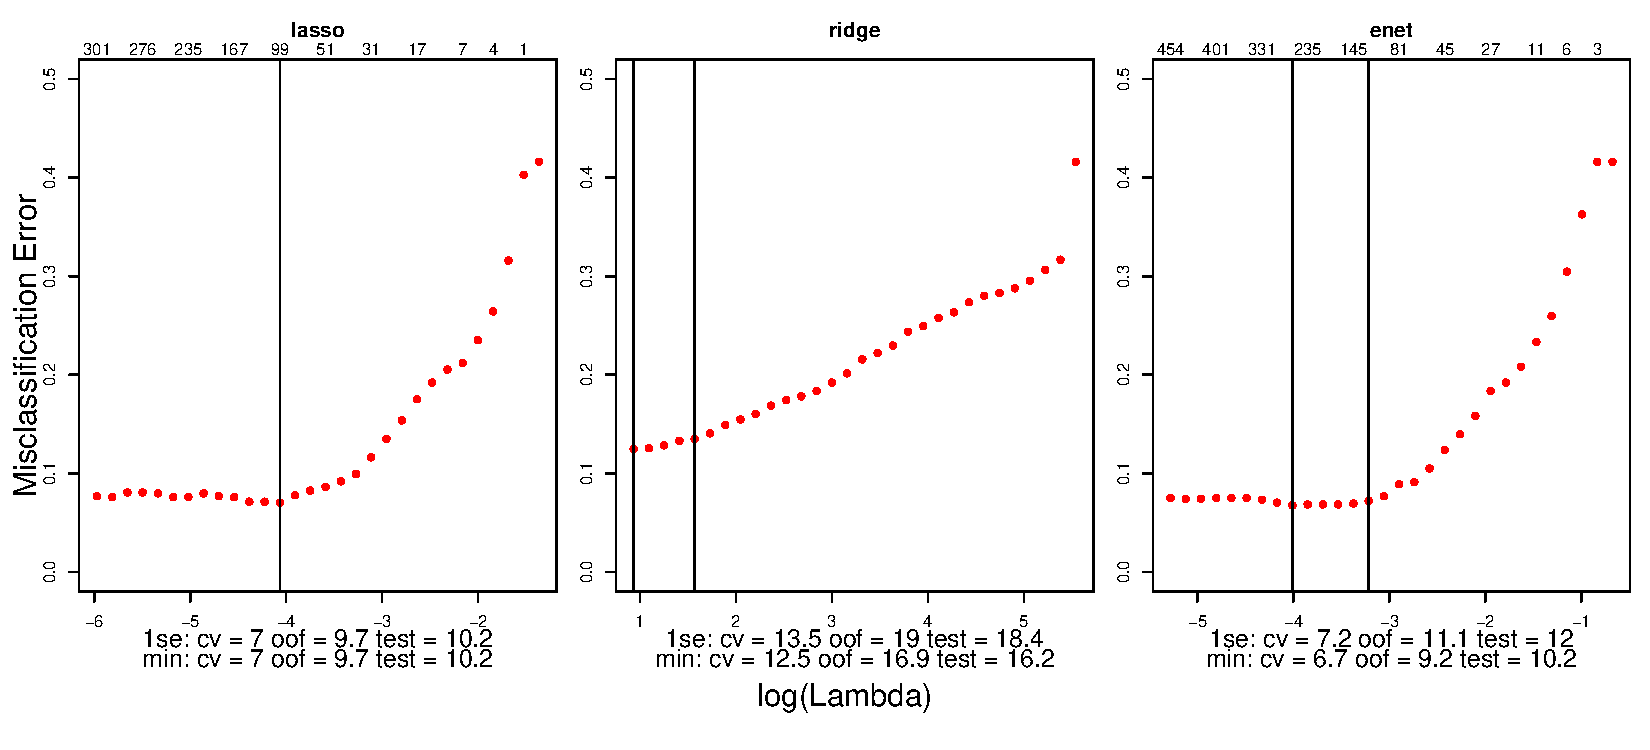
\includegraphics{Static/figures/lookFits-1.pdf}
\caption{\label{fig:lookFits}compare fits}
\end{figure}

\begin{Shaded}
\begin{Highlighting}[]
\NormalTok{errors\_frm <{-}}\StringTok{ }\KeywordTok{data.frame}\NormalTok{(}
  \DataTypeTok{lasso =}\NormalTok{ lasso\_errors\_mtx, }\DataTypeTok{ridge =}\NormalTok{ rifge\_errors\_mtx, }\DataTypeTok{enet =}\NormalTok{ enet\_errors\_mtx}
\NormalTok{)}
\KeywordTok{colnames}\NormalTok{(errors\_frm) <{-}}\StringTok{ }\KeywordTok{sub}\NormalTok{(}\StringTok{\textquotesingle{}}\CharTok{\textbackslash{}\textbackslash{}}\StringTok{.error\textquotesingle{}}\NormalTok{,}\StringTok{\textquotesingle{}\textquotesingle{}}\NormalTok{, }\KeywordTok{colnames}\NormalTok{(errors\_frm))}

\NormalTok{knitr}\OperatorTok{::}\KeywordTok{kable}\NormalTok{(}\KeywordTok{t}\NormalTok{(errors\_frm),}
 \DataTypeTok{caption =} \StringTok{\textquotesingle{}Misclassifiaction error rates\textquotesingle{}}\NormalTok{,}
 \DataTypeTok{digits=}\DecValTok{1}\NormalTok{) }\OperatorTok{\%>\%}\StringTok{ }
\StringTok{  }\NormalTok{kableExtra}\OperatorTok{::}\KeywordTok{kable\_styling}\NormalTok{(}\DataTypeTok{full\_width =}\NormalTok{ F)}
\end{Highlighting}
\end{Shaded}

\begin{table}

\caption{\label{tab:printErrors}Misclassifiaction error rates}
\centering
\begin{tabular}[t]{l|r|r|r}
\hline
  & p & train & test\\
\hline
lasso\_1se & 99 & 7.0 & 10.2\\
\hline
lasso\_min & 99 & 7.0 & 10.2\\
\hline
ridge\_1se & 15752 & 13.5 & 18.4\\
\hline
ridge\_min & 15752 & 12.5 & 16.2\\
\hline
enet\_1se & 118 & 7.2 & 12.0\\
\hline
enet\_min & 278 & 6.7 & 10.2\\
\hline
\end{tabular}
\end{table}

We see that the lasso and enet models do better than the ridge model.
The \emph{one standard error rule} (1se) lambda lasso fit is only slightly more parsimonious than the
\emph{1se} elastic net fit, but its test set accuracy is better.
The \emph{min} lambda models have lower test set error rates than
the more parsinomious \emph{1se} models in the ridge and elastice net case.
(for the lasso, 1se and minimum lambda rules give the same model).
The mimimum lambda elastic net fit performs as well as the lasso model,
but is much less parsimonious.

Note that the cv estiamtes of misclassification error produced by
the glmnet extraction method are \texttt{out-of-fold} estimated error rates.
In this particular dataset, these estimates of error are
optimistic in comparison the the test set error rates.

\hypertarget{the-relaxed-lasso-and-blended-mix-models}{%
\section{The relaxed lasso and blended mix models}\label{the-relaxed-lasso-and-blended-mix-models}}

Next we look at the so-called \texttt{relaxed\ lasso} model, and
the \texttt{blended\ mix} which is an optimized shrinkage
between the relaxed lasso and the regular lasso.
See \eqref{eq:blended} in Section \ref{modeling-background}.

\begin{Shaded}
\begin{Highlighting}[]
\KeywordTok{library}\NormalTok{(glmnet)}

\NormalTok{cv\_lassoR\_sum <{-}}\StringTok{ }\KeywordTok{print}\NormalTok{(cv\_lassoR)}
\end{Highlighting}
\end{Shaded}

\begin{verbatim}
## 
## Call:  glmnet::cv.glmnet(x = train_lcpm_mtx, y = train_group_vec, type.measure = "class",      foldid = train_foldid_vec, keep = T, relax = T, alpha = 1,      family = "binomial", nlambda = 30) 
## 
## Measure: Misclassification Error 
## 
##     Gamma Lambda Measure       SE Nonzero
## min   0.5 0.0379 0.06748 0.005274      35
## 1se   0.5 0.0379 0.06748 0.005274      35
\end{verbatim}

\begin{Shaded}
\begin{Highlighting}[]
\KeywordTok{plot}\NormalTok{(cv\_lassoR)}
\end{Highlighting}
\end{Shaded}

\begin{figure}
\centering
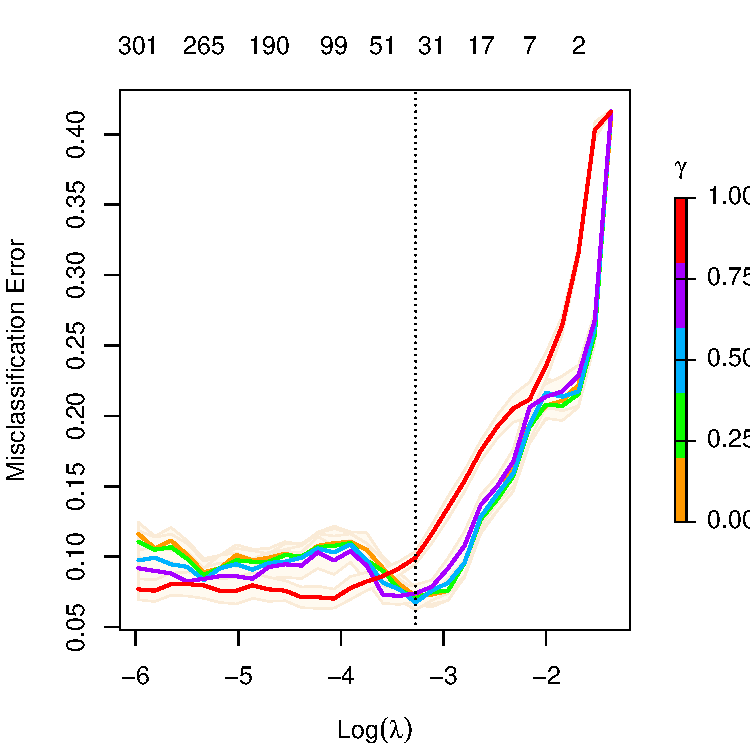
\includegraphics{Static/figures/lookLassoR-1.pdf}
\caption{\label{fig:lookLassoR}Relaxed lasso fit}
\end{figure}

\begin{Shaded}
\begin{Highlighting}[]
\CommentTok{\# only report  1se}
\NormalTok{ndx\_1se <{-}}\StringTok{ }\KeywordTok{match}\NormalTok{(cv\_lassoR}\OperatorTok{$}\NormalTok{lambda}\FloatTok{.1}\NormalTok{se, cv\_lassoR}\OperatorTok{$}\NormalTok{lambda)}
\NormalTok{ndx\_min <{-}}\StringTok{ }\KeywordTok{match}\NormalTok{(cv\_lassoR}\OperatorTok{$}\NormalTok{lambda.min, cv\_lassoR}\OperatorTok{$}\NormalTok{lambda)}

\CommentTok{\# only show 1se anyway}
\CommentTok{\# if(ndx\_1se != ndx\_min) stop("lambda.1se != lambda.min")}


\CommentTok{\# train oof data {-} NOT CLEAR WHY THESE DIFFER FROM CV ERRORS EXTRACTED FROM MODEL}
\CommentTok{\# Get relaxed lasso (gamma=0) oof error}
\NormalTok{train\_oofPred\_relaxed\_1se\_vec <{-}}\StringTok{ }\KeywordTok{ifelse}\NormalTok{(}
  \KeywordTok{logistic\_f}\NormalTok{(cv\_lassoR}\OperatorTok{$}\NormalTok{fit.preval[[}\StringTok{"g:0"}\NormalTok{]][, ndx\_1se]) }\OperatorTok{>}\StringTok{ }\FloatTok{0.5}\NormalTok{, }\StringTok{"HCC"}\NormalTok{, }\StringTok{"Control"}
\NormalTok{)}
\NormalTok{train\_oofPred\_relaxed\_1se\_error <{-}}\StringTok{ }\KeywordTok{mean}\NormalTok{(train\_oofPred\_relaxed\_1se\_vec }\OperatorTok{!=}\StringTok{ }\NormalTok{train\_group\_vec)}

\CommentTok{\# blended mix (gamma=0.5)}
\NormalTok{train\_oofPred\_blended\_1se\_vec <{-}}\StringTok{ }\KeywordTok{ifelse}\NormalTok{(}
  \KeywordTok{logistic\_f}\NormalTok{(cv\_lassoR}\OperatorTok{$}\NormalTok{fit.preval[[}\StringTok{"g:0.5"}\NormalTok{]][, ndx\_1se]) }\OperatorTok{>}\StringTok{ }\FloatTok{0.5}\NormalTok{, }\StringTok{"HCC"}\NormalTok{, }\StringTok{"Control"}
\NormalTok{)}
\NormalTok{train\_oofPred\_blended\_1se\_error <{-}}\StringTok{ }\KeywordTok{mean}\NormalTok{(train\_oofPred\_blended\_1se\_vec }\OperatorTok{!=}\StringTok{ }\NormalTok{train\_group\_vec)}


\CommentTok{\# Test set error {-} relaxed}
\NormalTok{test\_pred\_relaxed\_1se\_vec <{-}}\StringTok{ }\KeywordTok{predict}\NormalTok{(}
\NormalTok{  cv\_lassoR,}
  \DataTypeTok{newx =}\NormalTok{ test\_lcpm\_mtx,}
  \DataTypeTok{s =} \StringTok{"lambda.1se"}\NormalTok{,}
  \DataTypeTok{type =} \StringTok{"class"}\NormalTok{,}
  \DataTypeTok{gamma =} \DecValTok{0}
\NormalTok{)}
\NormalTok{test\_pred\_relaxed\_1se\_error <{-}}\StringTok{ }\KeywordTok{mean}\NormalTok{(test\_pred\_relaxed\_1se\_vec }\OperatorTok{!=}\StringTok{ }\NormalTok{test\_group\_vec)}

\CommentTok{\# Test set error {-} blended}
\NormalTok{test\_pred\_blended\_1se\_vec <{-}}\StringTok{ }\KeywordTok{predict}\NormalTok{(}
\NormalTok{  cv\_lassoR,}
  \DataTypeTok{newx =}\NormalTok{ test\_lcpm\_mtx,}
  \DataTypeTok{s =} \StringTok{"lambda.1se"}\NormalTok{,}
  \DataTypeTok{type =} \StringTok{"class"}\NormalTok{,}
  \DataTypeTok{gamma =} \FloatTok{0.5}
\NormalTok{)}
\NormalTok{test\_pred\_blended\_1se\_error <{-}}\StringTok{ }\KeywordTok{mean}\NormalTok{(test\_pred\_blended\_1se\_vec }\OperatorTok{!=}\StringTok{ }\NormalTok{test\_group\_vec)}


\NormalTok{cv\_lassoR\_1se\_error <{-}}\StringTok{ }\NormalTok{cv\_lassoR}\OperatorTok{$}\NormalTok{cvm[cv\_lassoR}\OperatorTok{$}\NormalTok{lambda}\OperatorTok{==}\NormalTok{cv\_lassoR}\OperatorTok{$}\NormalTok{lambda.min]}

\NormalTok{cv\_blended\_statlist <{-}}\StringTok{ }\NormalTok{cv\_lassoR}\OperatorTok{$}\NormalTok{relaxed}\OperatorTok{$}\NormalTok{statlist[[}\StringTok{\textquotesingle{}g:0.5\textquotesingle{}}\NormalTok{]]}
\NormalTok{cv\_blended\_1se\_error <{-}}\StringTok{ }\NormalTok{cv\_blended\_statlist}\OperatorTok{$}\NormalTok{cvm[cv\_blended\_statlist}\OperatorTok{$}\NormalTok{lambda}\OperatorTok{==}
\StringTok{   }\NormalTok{cv\_lassoR}\OperatorTok{$}\NormalTok{relaxed}\OperatorTok{$}\NormalTok{lambda}\FloatTok{.1}\NormalTok{se]}
 


\NormalTok{knitr}\OperatorTok{::}\KeywordTok{kable}\NormalTok{(}\KeywordTok{t}\NormalTok{(}\KeywordTok{data.frame}\NormalTok{(}
  \DataTypeTok{train\_relaxed  =}\NormalTok{ cv\_lassoR\_1se\_error,}
  \DataTypeTok{train\_blended  =}\NormalTok{ cv\_blended\_1se\_error,}
  \CommentTok{\#train\_relaxed\_oof = train\_oofPred\_relaxed\_1se\_error,}
  \CommentTok{\#train\_blended\_oof = train\_oofPred\_blended\_1se\_error,}
  \DataTypeTok{test\_relaxed  =}\NormalTok{ test\_pred\_relaxed\_1se\_error,}
  \DataTypeTok{test\_blended  =}\NormalTok{ test\_pred\_blended\_1se\_error}
\NormalTok{)) }\OperatorTok{*}\StringTok{ }\DecValTok{100}\NormalTok{,}
\DataTypeTok{digits =} \DecValTok{1}\NormalTok{,}
\DataTypeTok{caption =} \StringTok{"Relaxed lasso and blended mix error rates"}
\NormalTok{) }\OperatorTok{\%>\%}
\StringTok{  }\NormalTok{kableExtra}\OperatorTok{::}\KeywordTok{kable\_styling}\NormalTok{(}\DataTypeTok{full\_width =}\NormalTok{ F)}
\end{Highlighting}
\end{Shaded}

\begin{table}

\caption{\label{tab:lookLassoR2}Relaxed lasso and blended mix error rates}
\centering
\begin{tabular}[t]{l|r}
\hline
train\_relaxed & 7.0\\
\hline
train\_blended & 6.7\\
\hline
test\_relaxed & 10.9\\
\hline
test\_blended & 10.2\\
\hline
\end{tabular}
\end{table}

The relaxed lasso and blended mix error rates are comparable to the
regular lasso fit error rate. We see here too that the reported cv
error rates are optimistic.

The \emph{1se} lambda rule applied to the relaxed lasso fit selected a model with
\(99\) features,
while for the blended mix model
(See \eqref{eq:blended} in Section \ref{modeling-background})
the \emph{1se} lambda rule selected
\(35\) features (vertical
dotted reference line in Figure \ref{fig:lookLassoR}).
This feature is pointed out in the
\href{https://cran.r-project.org/web/packages/glmnet/vignettes/relax.pdf}{glmnet 3.0 vignette}:
\emph{The debiasing will potentially improve prediction performance,
and CV will typically select a model with a smaller number of variables.}

\hypertarget{examination-of-sensitivity-vs-specificity}{%
\section{Examination of sensitivity vs specificity}\label{examination-of-sensitivity-vs-specificity}}

In the results above we reported error rates without inspecting the
sensitivity versus specificity trade-off. ROC curves can be examined
to get a sense of the trade-off.

\hypertarget{training-data-out-of-fold-roc-curves}{%
\subsection{Training data out-of-fold ROC curves}\label{training-data-out-of-fold-roc-curves}}

\begin{Shaded}
\begin{Highlighting}[]
\CommentTok{\# train}
\CommentTok{\# lasso}
\NormalTok{ndx\_1se <{-}}\StringTok{ }\KeywordTok{match}\NormalTok{(cv\_lasso}\OperatorTok{$}\NormalTok{lambda}\FloatTok{.1}\NormalTok{se,cv\_lasso}\OperatorTok{$}\NormalTok{lambda)}
\NormalTok{train\_lasso\_oofProb\_vec <{-}}\StringTok{ }\KeywordTok{logistic\_f}\NormalTok{(cv\_lasso}\OperatorTok{$}\NormalTok{fit.preval[,ndx\_1se])}
\NormalTok{train\_lasso\_roc <{-}}\StringTok{ }\NormalTok{pROC}\OperatorTok{::}\KeywordTok{roc}\NormalTok{(}
 \DataTypeTok{response =} \KeywordTok{as.numeric}\NormalTok{(train\_group\_vec}\OperatorTok{==}\StringTok{\textquotesingle{}HCC\textquotesingle{}}\NormalTok{),}
 \DataTypeTok{predictor =}\NormalTok{ train\_lasso\_oofProb\_vec)}
\end{Highlighting}
\end{Shaded}

\begin{verbatim}
## Setting levels: control = 0, case = 1
\end{verbatim}

\begin{verbatim}
## Setting direction: controls < cases
\end{verbatim}

\begin{Shaded}
\begin{Highlighting}[]
\CommentTok{\# enet}
\NormalTok{ndx\_1se <{-}}\StringTok{ }\KeywordTok{match}\NormalTok{(cv\_enet}\OperatorTok{$}\NormalTok{lambda}\FloatTok{.1}\NormalTok{se,cv\_enet}\OperatorTok{$}\NormalTok{lambda)}
\NormalTok{train\_enet\_oofProb\_vec <{-}}\StringTok{ }\KeywordTok{logistic\_f}\NormalTok{(cv\_enet}\OperatorTok{$}\NormalTok{fit.preval[,ndx\_1se])}
\NormalTok{train\_enet\_roc <{-}}\StringTok{ }\NormalTok{pROC}\OperatorTok{::}\KeywordTok{roc}\NormalTok{(}
 \DataTypeTok{response =} \KeywordTok{as.numeric}\NormalTok{(train\_group\_vec}\OperatorTok{==}\StringTok{\textquotesingle{}HCC\textquotesingle{}}\NormalTok{),}
 \DataTypeTok{predictor =}\NormalTok{ train\_enet\_oofProb\_vec)}
\end{Highlighting}
\end{Shaded}

\begin{verbatim}
## Setting levels: control = 0, case = 1
## Setting direction: controls < cases
\end{verbatim}

\begin{Shaded}
\begin{Highlighting}[]
\CommentTok{\# lasso {-} relaxed}
\NormalTok{ndx\_1se <{-}}\StringTok{ }\KeywordTok{match}\NormalTok{(cv\_lassoR}\OperatorTok{$}\NormalTok{lambda}\FloatTok{.1}\NormalTok{se,cv\_lassoR}\OperatorTok{$}\NormalTok{lambda)}
\NormalTok{train\_relaxed\_oofProb\_vec <{-}}\StringTok{ }\KeywordTok{logistic\_f}\NormalTok{(cv\_lassoR}\OperatorTok{$}\NormalTok{fit.preval[[}\StringTok{\textquotesingle{}g:0\textquotesingle{}}\NormalTok{]][,ndx\_1se])}
\NormalTok{train\_relaxed\_roc <{-}}\StringTok{ }\NormalTok{pROC}\OperatorTok{::}\KeywordTok{roc}\NormalTok{(}
 \DataTypeTok{response =} \KeywordTok{as.numeric}\NormalTok{(train\_group\_vec}\OperatorTok{==}\StringTok{\textquotesingle{}HCC\textquotesingle{}}\NormalTok{),}
 \DataTypeTok{predictor =}\NormalTok{ train\_relaxed\_oofProb\_vec)}
\end{Highlighting}
\end{Shaded}

\begin{verbatim}
## Setting levels: control = 0, case = 1
## Setting direction: controls < cases
\end{verbatim}

\begin{Shaded}
\begin{Highlighting}[]
\CommentTok{\# blended mix (gamma=0.5)}
\NormalTok{ndx\_1se <{-}}\StringTok{ }\KeywordTok{match}\NormalTok{(cv\_lassoR}\OperatorTok{$}\NormalTok{lambda}\FloatTok{.1}\NormalTok{se,cv\_lassoR}\OperatorTok{$}\NormalTok{lambda)}
\NormalTok{train\_blended\_oofProb\_vec <{-}}\StringTok{ }\KeywordTok{logistic\_f}\NormalTok{(cv\_lassoR}\OperatorTok{$}\NormalTok{fit.preval[[}\StringTok{\textquotesingle{}g:0.5\textquotesingle{}}\NormalTok{]][,ndx\_1se])}
\NormalTok{train\_blended\_roc <{-}}\StringTok{ }\NormalTok{pROC}\OperatorTok{::}\KeywordTok{roc}\NormalTok{(}
 \DataTypeTok{response =} \KeywordTok{as.numeric}\NormalTok{(train\_group\_vec}\OperatorTok{==}\StringTok{\textquotesingle{}HCC\textquotesingle{}}\NormalTok{),}
 \DataTypeTok{predictor =}\NormalTok{ train\_blended\_oofProb\_vec)}
\end{Highlighting}
\end{Shaded}

\begin{verbatim}
## Setting levels: control = 0, case = 1
## Setting direction: controls < cases
\end{verbatim}

\begin{Shaded}
\begin{Highlighting}[]
\KeywordTok{plot}\NormalTok{(train\_lasso\_roc, }\DataTypeTok{col=}\NormalTok{col\_vec[}\DecValTok{1}\NormalTok{])}
\KeywordTok{lines}\NormalTok{(train\_enet\_roc, }\DataTypeTok{col=}\NormalTok{col\_vec[}\DecValTok{2}\NormalTok{])}
\KeywordTok{lines}\NormalTok{(train\_relaxed\_roc, }\DataTypeTok{col=}\NormalTok{col\_vec[}\DecValTok{3}\NormalTok{])}
\KeywordTok{lines}\NormalTok{(train\_blended\_roc, }\DataTypeTok{col=}\NormalTok{col\_vec[}\DecValTok{4}\NormalTok{])}

\KeywordTok{legend}\NormalTok{(}\StringTok{\textquotesingle{}bottomright\textquotesingle{}}\NormalTok{, }\DataTypeTok{title=}\StringTok{\textquotesingle{}AUC\textquotesingle{}}\NormalTok{,}
 \DataTypeTok{legend=}\KeywordTok{c}\NormalTok{(}
  \KeywordTok{paste}\NormalTok{(}\StringTok{\textquotesingle{}lasso =\textquotesingle{}}\NormalTok{, }\KeywordTok{round}\NormalTok{(train\_lasso\_roc[[}\StringTok{\textquotesingle{}auc\textquotesingle{}}\NormalTok{]],}\DecValTok{3}\NormalTok{)),}
  \KeywordTok{paste}\NormalTok{(}\StringTok{\textquotesingle{}enet =\textquotesingle{}}\NormalTok{, }\KeywordTok{round}\NormalTok{(train\_enet\_roc[[}\StringTok{\textquotesingle{}auc\textquotesingle{}}\NormalTok{]],}\DecValTok{3}\NormalTok{)),}
  \KeywordTok{paste}\NormalTok{(}\StringTok{\textquotesingle{}relaxed =\textquotesingle{}}\NormalTok{, }\KeywordTok{round}\NormalTok{(train\_relaxed\_roc[[}\StringTok{\textquotesingle{}auc\textquotesingle{}}\NormalTok{]],}\DecValTok{3}\NormalTok{)),}
  \KeywordTok{paste}\NormalTok{(}\StringTok{\textquotesingle{}blended =\textquotesingle{}}\NormalTok{, }\KeywordTok{round}\NormalTok{(train\_blended\_roc[[}\StringTok{\textquotesingle{}auc\textquotesingle{}}\NormalTok{]],}\DecValTok{3}\NormalTok{))}
\NormalTok{ ),}
 \DataTypeTok{text.col =}\NormalTok{ col\_vec[}\DecValTok{1}\OperatorTok{:}\DecValTok{4}\NormalTok{],}
 \DataTypeTok{bty=}\StringTok{\textquotesingle{}n\textquotesingle{}}
\NormalTok{)}
\end{Highlighting}
\end{Shaded}

\begin{figure}
\centering
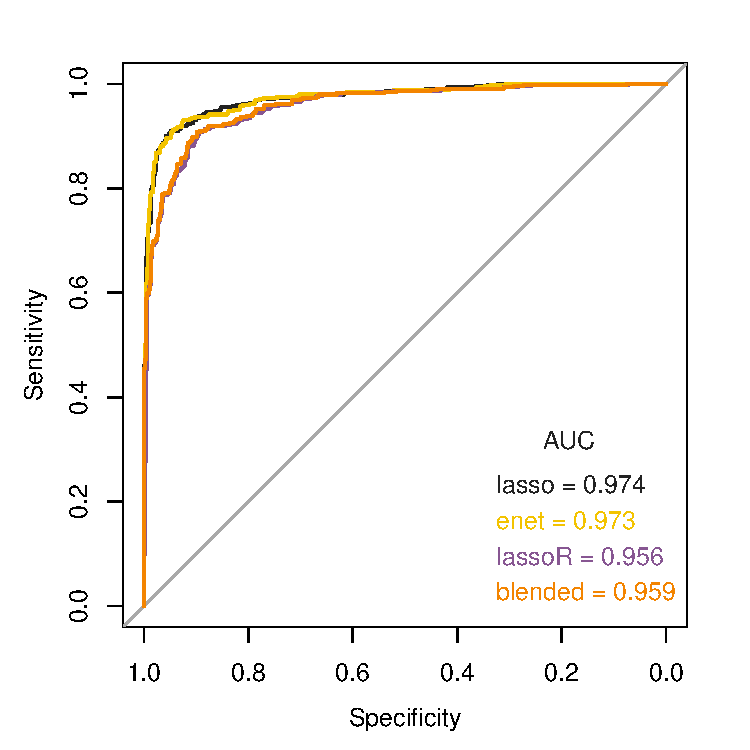
\includegraphics{Static/figures/trainROC-1.pdf}
\caption{\label{fig:trainROC}Train data out-of-sample ROCs}
\end{figure}

Compare thresholds for 90\% Specificity:

\begin{Shaded}
\begin{Highlighting}[]
\NormalTok{ lasso\_ndx <{-}}\StringTok{ }\KeywordTok{with}\NormalTok{(}\KeywordTok{as.data.frame}\NormalTok{(pROC}\OperatorTok{::}\KeywordTok{coords}\NormalTok{(train\_lasso\_roc, }\DataTypeTok{transpose=}\NormalTok{F)), }
   \KeywordTok{min}\NormalTok{(}\KeywordTok{which}\NormalTok{(specificity }\OperatorTok{>=}\StringTok{ }\FloatTok{0.9}\NormalTok{)))}

\NormalTok{ enet\_ndx <{-}}\StringTok{ }\KeywordTok{with}\NormalTok{(}\KeywordTok{as.data.frame}\NormalTok{(pROC}\OperatorTok{::}\KeywordTok{coords}\NormalTok{(train\_enet\_roc, }\DataTypeTok{transpose=}\NormalTok{F)), }
   \KeywordTok{min}\NormalTok{(}\KeywordTok{which}\NormalTok{(specificity }\OperatorTok{>=}\StringTok{ }\FloatTok{0.9}\NormalTok{)))}

\NormalTok{ lassoR\_ndx <{-}}\StringTok{ }\KeywordTok{with}\NormalTok{(}\KeywordTok{as.data.frame}\NormalTok{(pROC}\OperatorTok{::}\KeywordTok{coords}\NormalTok{(train\_relaxed\_roc, }\DataTypeTok{transpose=}\NormalTok{F)), }
   \KeywordTok{min}\NormalTok{(}\KeywordTok{which}\NormalTok{(specificity }\OperatorTok{>=}\StringTok{ }\FloatTok{0.9}\NormalTok{)))}

\NormalTok{ blended\_ndx <{-}}\StringTok{ }\KeywordTok{with}\NormalTok{(}\KeywordTok{as.data.frame}\NormalTok{(pROC}\OperatorTok{::}\KeywordTok{coords}\NormalTok{(train\_blended\_roc, }\DataTypeTok{transpose=}\NormalTok{F)), }
   \KeywordTok{min}\NormalTok{(}\KeywordTok{which}\NormalTok{(specificity }\OperatorTok{>=}\StringTok{ }\FloatTok{0.9}\NormalTok{)))}

\NormalTok{  spec90\_frm <{-}}\StringTok{ }\KeywordTok{data.frame}\NormalTok{(}\KeywordTok{rbind}\NormalTok{(}
  \DataTypeTok{lasso=}\KeywordTok{as.data.frame}\NormalTok{(pROC}\OperatorTok{::}\KeywordTok{coords}\NormalTok{(train\_lasso\_roc, }\DataTypeTok{transpose=}\NormalTok{F))[lasso\_ndx,],}
  \DataTypeTok{enet=}\KeywordTok{as.data.frame}\NormalTok{(pROC}\OperatorTok{::}\KeywordTok{coords}\NormalTok{(train\_enet\_roc, }\DataTypeTok{transpose=}\NormalTok{F))[enet\_ndx,],}
  \DataTypeTok{relaxed=}\KeywordTok{as.data.frame}\NormalTok{(pROC}\OperatorTok{::}\KeywordTok{coords}\NormalTok{(train\_relaxed\_roc, }\DataTypeTok{transpose=}\NormalTok{F))[lassoR\_ndx,],}
  \DataTypeTok{blended=}\KeywordTok{as.data.frame}\NormalTok{(pROC}\OperatorTok{::}\KeywordTok{coords}\NormalTok{(train\_blended\_roc, }\DataTypeTok{transpose=}\NormalTok{F))[blended\_ndx,]}
\NormalTok{ ))}


\NormalTok{knitr}\OperatorTok{::}\KeywordTok{kable}\NormalTok{(spec90\_frm,}
  \DataTypeTok{digits=}\DecValTok{3}\NormalTok{,}
  \DataTypeTok{caption=}\StringTok{"Specificity = .90 Coordinates"}
\NormalTok{) }\OperatorTok{\%>\%}
\StringTok{  }\NormalTok{kableExtra}\OperatorTok{::}\KeywordTok{kable\_styling}\NormalTok{(}\DataTypeTok{full\_width =}\NormalTok{ F)}
\end{Highlighting}
\end{Shaded}

\begin{table}

\caption{\label{tab:thresh90}Specificity = .90 Coordinates}
\centering
\begin{tabular}[t]{l|r|r|r}
\hline
  & threshold & specificity & sensitivity\\
\hline
lasso & 0.337 & 0.9 & 0.932\\
\hline
enet & 0.347 & 0.9 & 0.937\\
\hline
relaxed & 0.003 & 0.9 & 0.894\\
\hline
blended & 0.031 & 0.9 & 0.899\\
\hline
\end{tabular}
\end{table}

This is strange.

\begin{Shaded}
\begin{Highlighting}[]
\KeywordTok{par}\NormalTok{(}\DataTypeTok{mfrow =} \KeywordTok{c}\NormalTok{(}\DecValTok{2}\NormalTok{, }\DecValTok{2}\NormalTok{), }\DataTypeTok{mar =} \KeywordTok{c}\NormalTok{(}\DecValTok{3}\NormalTok{, }\DecValTok{3}\NormalTok{, }\DecValTok{2}\NormalTok{, }\DecValTok{1}\NormalTok{), }\DataTypeTok{oma =} \KeywordTok{c}\NormalTok{(}\DecValTok{2}\NormalTok{, }\DecValTok{2}\NormalTok{, }\DecValTok{2}\NormalTok{, }\DecValTok{2}\NormalTok{))}

\CommentTok{\# lasso}
\KeywordTok{plot}\NormalTok{(}\KeywordTok{density}\NormalTok{(train\_lasso\_oofProb\_vec[train\_group\_vec }\OperatorTok{==}\StringTok{ "Control"}\NormalTok{]),}
  \DataTypeTok{xlim =} \KeywordTok{c}\NormalTok{(}\DecValTok{0}\NormalTok{, }\DecValTok{1}\NormalTok{), }\DataTypeTok{main =} \StringTok{""}\NormalTok{, }\DataTypeTok{xlab =} \StringTok{""}\NormalTok{, }\DataTypeTok{ylab =} \StringTok{""}\NormalTok{, }\DataTypeTok{col =} \StringTok{"green"}
\NormalTok{)}
\KeywordTok{lines}\NormalTok{(}\KeywordTok{density}\NormalTok{(train\_lasso\_oofProb\_vec[train\_group\_vec }\OperatorTok{==}\StringTok{ "HCC"}\NormalTok{]),}
  \DataTypeTok{col =} \StringTok{"red"}
\NormalTok{)}
\KeywordTok{title}\NormalTok{(}\StringTok{"lasso"}\NormalTok{)}
\KeywordTok{legend}\NormalTok{(}\StringTok{"topright"}\NormalTok{, }\DataTypeTok{legend =} \KeywordTok{c}\NormalTok{(}\StringTok{"Control"}\NormalTok{, }\StringTok{"HCC"}\NormalTok{), }\DataTypeTok{text.col =} \KeywordTok{c}\NormalTok{(}\StringTok{"green"}\NormalTok{, }\StringTok{"red"}\NormalTok{))}

\CommentTok{\# enet}
\KeywordTok{plot}\NormalTok{(}\KeywordTok{density}\NormalTok{(train\_enet\_oofProb\_vec[train\_group\_vec }\OperatorTok{==}\StringTok{ "Control"}\NormalTok{]),}
  \DataTypeTok{xlim =} \KeywordTok{c}\NormalTok{(}\DecValTok{0}\NormalTok{, }\DecValTok{1}\NormalTok{), }\DataTypeTok{main =} \StringTok{""}\NormalTok{, }\DataTypeTok{xlab =} \StringTok{""}\NormalTok{, }\DataTypeTok{ylab =} \StringTok{""}\NormalTok{, }\DataTypeTok{col =} \StringTok{"green"}
\NormalTok{)}
\KeywordTok{lines}\NormalTok{(}\KeywordTok{density}\NormalTok{(train\_enet\_oofProb\_vec[train\_group\_vec }\OperatorTok{==}\StringTok{ "HCC"}\NormalTok{]),}
  \DataTypeTok{col =} \StringTok{"red"}
\NormalTok{)}
\KeywordTok{title}\NormalTok{(}\StringTok{"enet"}\NormalTok{)}

\CommentTok{\# lassoR}
\KeywordTok{plot}\NormalTok{(}\KeywordTok{density}\NormalTok{(train\_relaxed\_oofProb\_vec[train\_group\_vec }\OperatorTok{==}\StringTok{ "Control"}\NormalTok{]),}
  \DataTypeTok{xlim =} \KeywordTok{c}\NormalTok{(}\DecValTok{0}\NormalTok{, }\DecValTok{1}\NormalTok{), }\DataTypeTok{main =} \StringTok{""}\NormalTok{, }\DataTypeTok{xlab =} \StringTok{""}\NormalTok{, }\DataTypeTok{ylab =} \StringTok{""}\NormalTok{, }\DataTypeTok{col =} \StringTok{"green"}
\NormalTok{)}
\KeywordTok{lines}\NormalTok{(}\KeywordTok{density}\NormalTok{(train\_relaxed\_oofProb\_vec[train\_group\_vec }\OperatorTok{==}\StringTok{ "HCC"}\NormalTok{]),}
  \DataTypeTok{col =} \StringTok{"red"}
\NormalTok{)}
\KeywordTok{title}\NormalTok{(}\StringTok{"lassoR"}\NormalTok{)}

\CommentTok{\# blended}
\KeywordTok{plot}\NormalTok{(}\KeywordTok{density}\NormalTok{(train\_blended\_oofProb\_vec[train\_group\_vec }\OperatorTok{==}\StringTok{ "Control"}\NormalTok{]),}
  \DataTypeTok{xlim =} \KeywordTok{c}\NormalTok{(}\DecValTok{0}\NormalTok{, }\DecValTok{1}\NormalTok{), }\DataTypeTok{main =} \StringTok{""}\NormalTok{, }\DataTypeTok{xlab =} \StringTok{""}\NormalTok{, }\DataTypeTok{ylab =} \StringTok{""}\NormalTok{, }\DataTypeTok{col =} \StringTok{"green"}
\NormalTok{)}
\KeywordTok{lines}\NormalTok{(}\KeywordTok{density}\NormalTok{(train\_blended\_oofProb\_vec[train\_group\_vec }\OperatorTok{==}\StringTok{ "HCC"}\NormalTok{]),}
  \DataTypeTok{col =} \StringTok{"red"}
\NormalTok{)}
\KeywordTok{title}\NormalTok{(}\StringTok{"blended"}\NormalTok{)}

\KeywordTok{mtext}\NormalTok{(}\DataTypeTok{side =} \DecValTok{1}\NormalTok{, }\DataTypeTok{outer =}\NormalTok{ T, }\StringTok{"out{-}of{-}fold predicted probability"}\NormalTok{, }\DataTypeTok{cex =} \FloatTok{1.25}\NormalTok{)}
\KeywordTok{mtext}\NormalTok{(}\DataTypeTok{side =} \DecValTok{2}\NormalTok{, }\DataTypeTok{outer =}\NormalTok{ T, }\StringTok{"density"}\NormalTok{, }\DataTypeTok{cex =} \FloatTok{1.25}\NormalTok{)}
\end{Highlighting}
\end{Shaded}

\begin{figure}
\centering
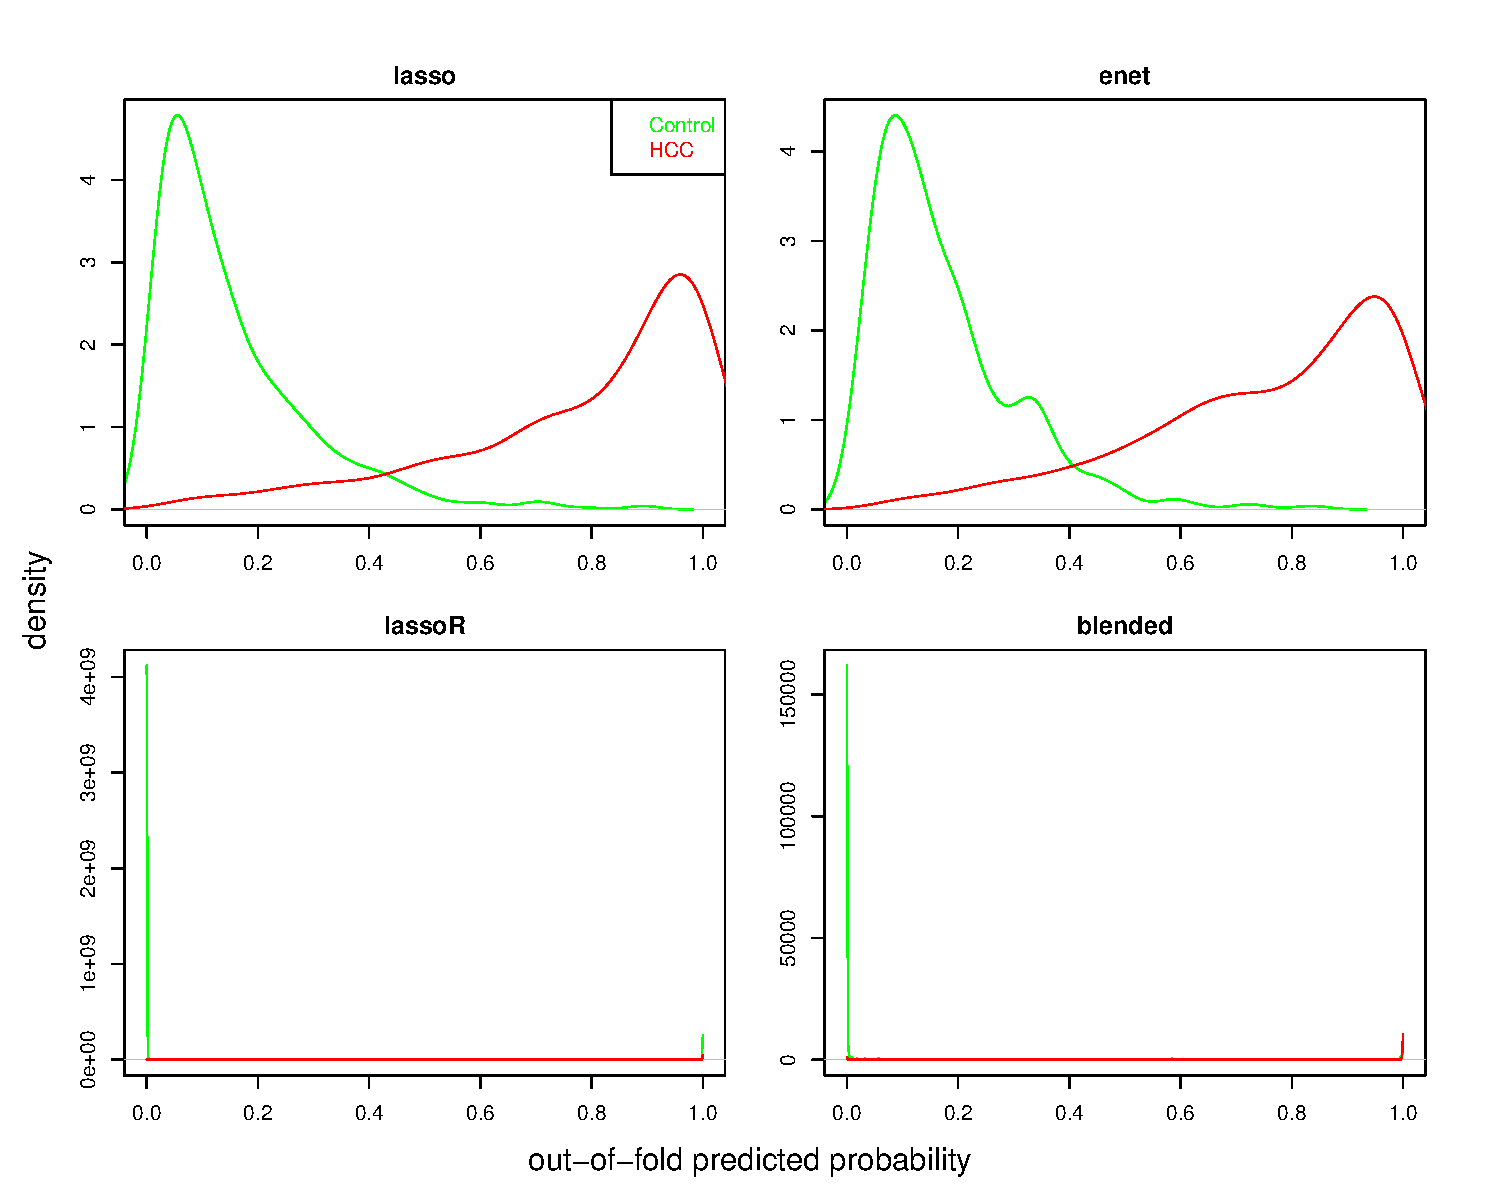
\includegraphics{Static/figures/trainOOFprops-1.pdf}
\caption{\label{fig:trainOOFprops}Train data out-of-fold predicted probabilities}
\end{figure}

The relaxed lasso fit results in essentially dichotomized predicted probability
distribution - predicted probabilities are very close to 0 or 1.

Look at test data ROC curves.

\begin{Shaded}
\begin{Highlighting}[]
\CommentTok{\# plot all}
\KeywordTok{plot}\NormalTok{(test\_lasso\_roc, }\DataTypeTok{col =}\NormalTok{ col\_vec[}\DecValTok{1}\NormalTok{])}
\KeywordTok{lines}\NormalTok{(test\_enet\_roc, }\DataTypeTok{col =}\NormalTok{ col\_vec[}\DecValTok{2}\NormalTok{])}
\KeywordTok{lines}\NormalTok{(test\_relaxed\_roc, }\DataTypeTok{col =}\NormalTok{ col\_vec[}\DecValTok{3}\NormalTok{])}
\KeywordTok{lines}\NormalTok{(test\_blended\_roc, }\DataTypeTok{col =}\NormalTok{ col\_vec[}\DecValTok{4}\NormalTok{])}

\KeywordTok{legend}\NormalTok{(}\StringTok{"bottomright"}\NormalTok{,}
  \DataTypeTok{title =} \StringTok{"AUC"}\NormalTok{,}
  \DataTypeTok{legend =} \KeywordTok{c}\NormalTok{(}
    \KeywordTok{paste}\NormalTok{(}\StringTok{"lasso ="}\NormalTok{, }\KeywordTok{round}\NormalTok{(test\_lasso\_roc[[}\StringTok{"auc"}\NormalTok{]], }\DecValTok{3}\NormalTok{)),}
    \KeywordTok{paste}\NormalTok{(}\StringTok{"enet ="}\NormalTok{, }\KeywordTok{round}\NormalTok{(test\_enet\_roc[[}\StringTok{"auc"}\NormalTok{]], }\DecValTok{3}\NormalTok{)),}
    \KeywordTok{paste}\NormalTok{(}\StringTok{"relaxed ="}\NormalTok{, }\KeywordTok{round}\NormalTok{(test\_relaxed\_roc[[}\StringTok{"auc"}\NormalTok{]], }\DecValTok{3}\NormalTok{)),}
    \KeywordTok{paste}\NormalTok{(}\StringTok{"blended ="}\NormalTok{, }\KeywordTok{round}\NormalTok{(test\_blended\_roc[[}\StringTok{"auc"}\NormalTok{]], }\DecValTok{3}\NormalTok{))}
\NormalTok{  ),}
  \DataTypeTok{text.col =}\NormalTok{ col\_vec[}\DecValTok{1}\OperatorTok{:}\DecValTok{4}\NormalTok{],}
  \DataTypeTok{bty=}\StringTok{\textquotesingle{}n\textquotesingle{}}
\NormalTok{)}
\end{Highlighting}
\end{Shaded}

\begin{figure}
\centering
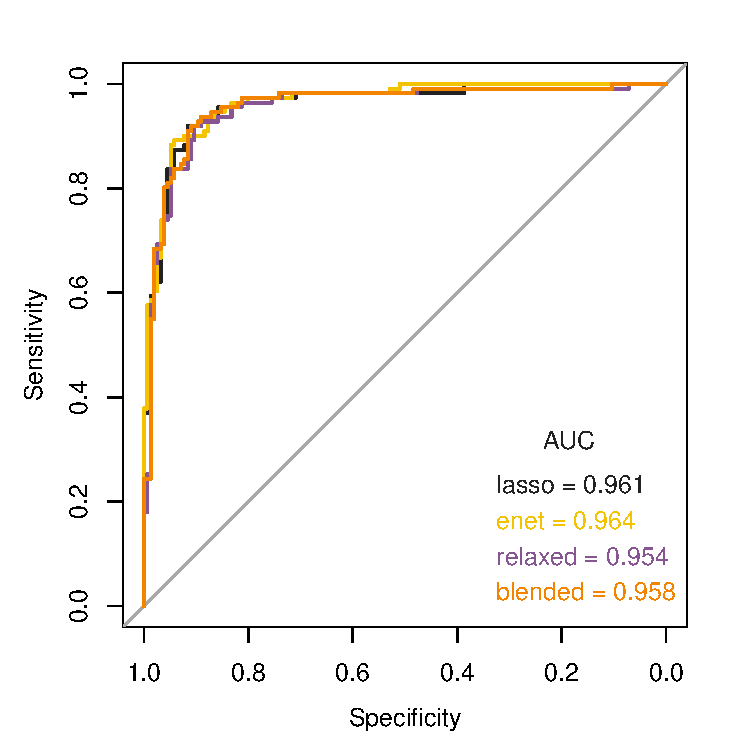
\includegraphics{Static/figures/testROC2-1.pdf}
\caption{\label{fig:testROC2}Test data out-of-sample ROCs}
\end{figure}

Look at densities of predicted probabilities.

\begin{Shaded}
\begin{Highlighting}[]
\KeywordTok{par}\NormalTok{(}\DataTypeTok{mfrow =} \KeywordTok{c}\NormalTok{(}\DecValTok{2}\NormalTok{, }\DecValTok{2}\NormalTok{), }\DataTypeTok{mar =} \KeywordTok{c}\NormalTok{(}\DecValTok{3}\NormalTok{, }\DecValTok{3}\NormalTok{, }\DecValTok{2}\NormalTok{, }\DecValTok{1}\NormalTok{), }\DataTypeTok{oma =} \KeywordTok{c}\NormalTok{(}\DecValTok{2}\NormalTok{, }\DecValTok{2}\NormalTok{, }\DecValTok{2}\NormalTok{, }\DecValTok{2}\NormalTok{))}

\CommentTok{\# lasso}
\KeywordTok{plot}\NormalTok{(}\KeywordTok{density}\NormalTok{(test\_lasso\_predProb\_vec[test\_group\_vec }\OperatorTok{==}\StringTok{ "Control"}\NormalTok{]),}
  \DataTypeTok{xlim =} \KeywordTok{c}\NormalTok{(}\DecValTok{0}\NormalTok{, }\DecValTok{1}\NormalTok{), }\DataTypeTok{main =} \StringTok{""}\NormalTok{, }\DataTypeTok{xlab =} \StringTok{""}\NormalTok{, }\DataTypeTok{ylab =} \StringTok{""}\NormalTok{, }\DataTypeTok{col =} \StringTok{"green"}
\NormalTok{)}
\KeywordTok{lines}\NormalTok{(}\KeywordTok{density}\NormalTok{(test\_lasso\_predProb\_vec[test\_group\_vec }\OperatorTok{==}\StringTok{ "HCC"}\NormalTok{]),}
  \DataTypeTok{col =} \StringTok{"red"}
\NormalTok{)}
\KeywordTok{title}\NormalTok{(}\StringTok{"lasso"}\NormalTok{)}
\KeywordTok{legend}\NormalTok{(}\StringTok{"topright"}\NormalTok{, }\DataTypeTok{legend =} \KeywordTok{c}\NormalTok{(}\StringTok{"Control"}\NormalTok{, }\StringTok{"HCC"}\NormalTok{), }\DataTypeTok{text.col =} \KeywordTok{c}\NormalTok{(}\StringTok{"green"}\NormalTok{, }\StringTok{"red"}\NormalTok{))}

\CommentTok{\# enet}
\KeywordTok{plot}\NormalTok{(}\KeywordTok{density}\NormalTok{(test\_enet\_predProb\_vec[test\_group\_vec }\OperatorTok{==}\StringTok{ "Control"}\NormalTok{]),}
  \DataTypeTok{xlim =} \KeywordTok{c}\NormalTok{(}\DecValTok{0}\NormalTok{, }\DecValTok{1}\NormalTok{), }\DataTypeTok{main =} \StringTok{""}\NormalTok{, }\DataTypeTok{xlab =} \StringTok{""}\NormalTok{, }\DataTypeTok{ylab =} \StringTok{""}\NormalTok{, }\DataTypeTok{col =} \StringTok{"green"}
\NormalTok{)}
\KeywordTok{lines}\NormalTok{(}\KeywordTok{density}\NormalTok{(test\_enet\_predProb\_vec[test\_group\_vec }\OperatorTok{==}\StringTok{ "HCC"}\NormalTok{]),}
  \DataTypeTok{col =} \StringTok{"red"}
\NormalTok{)}
\KeywordTok{title}\NormalTok{(}\StringTok{"enet"}\NormalTok{)}

\CommentTok{\# relaxed}
\KeywordTok{plot}\NormalTok{(}\KeywordTok{density}\NormalTok{(test\_relaxed\_predProb\_vec[test\_group\_vec }\OperatorTok{==}\StringTok{ "Control"}\NormalTok{]),}
  \DataTypeTok{xlim =} \KeywordTok{c}\NormalTok{(}\DecValTok{0}\NormalTok{, }\DecValTok{1}\NormalTok{), }\DataTypeTok{main =} \StringTok{""}\NormalTok{, }\DataTypeTok{xlab =} \StringTok{""}\NormalTok{, }\DataTypeTok{ylab =} \StringTok{""}\NormalTok{, }\DataTypeTok{col =} \StringTok{"green"}
\NormalTok{)}
\KeywordTok{lines}\NormalTok{(}\KeywordTok{density}\NormalTok{(test\_relaxed\_predProb\_vec[test\_group\_vec }\OperatorTok{==}\StringTok{ "HCC"}\NormalTok{]),}
  \DataTypeTok{col =} \StringTok{"red"}
\NormalTok{)}
\KeywordTok{title}\NormalTok{(}\StringTok{"relaxed"}\NormalTok{)}

\CommentTok{\#sapply(split(test\_relaxed\_predProb\_vec, test\_group\_vec), summary)}


\CommentTok{\# blended}
\KeywordTok{plot}\NormalTok{(}\KeywordTok{density}\NormalTok{(test\_blended\_predProb\_vec[test\_group\_vec }\OperatorTok{==}\StringTok{ "Control"}\NormalTok{]),}
  \DataTypeTok{xlim =} \KeywordTok{c}\NormalTok{(}\DecValTok{0}\NormalTok{, }\DecValTok{1}\NormalTok{), }\DataTypeTok{main =} \StringTok{""}\NormalTok{, }\DataTypeTok{xlab =} \StringTok{""}\NormalTok{, }\DataTypeTok{ylab =} \StringTok{""}\NormalTok{, }\DataTypeTok{col =} \StringTok{"green"}
\NormalTok{)}
\KeywordTok{lines}\NormalTok{(}\KeywordTok{density}\NormalTok{(test\_blended\_predProb\_vec[test\_group\_vec }\OperatorTok{==}\StringTok{ "HCC"}\NormalTok{]),}
  \DataTypeTok{col =} \StringTok{"red"}
\NormalTok{)}
\KeywordTok{title}\NormalTok{(}\StringTok{"blended"}\NormalTok{)}

\KeywordTok{mtext}\NormalTok{(}\DataTypeTok{side =} \DecValTok{1}\NormalTok{, }\DataTypeTok{outer =}\NormalTok{ T, }\StringTok{"test set predicted probability"}\NormalTok{, }\DataTypeTok{cex =} \FloatTok{1.25}\NormalTok{)}
\KeywordTok{mtext}\NormalTok{(}\DataTypeTok{side =} \DecValTok{2}\NormalTok{, }\DataTypeTok{outer =}\NormalTok{ T, }\StringTok{"density"}\NormalTok{, }\DataTypeTok{cex =} \FloatTok{1.25}\NormalTok{)}
\end{Highlighting}
\end{Shaded}

\begin{figure}
\centering
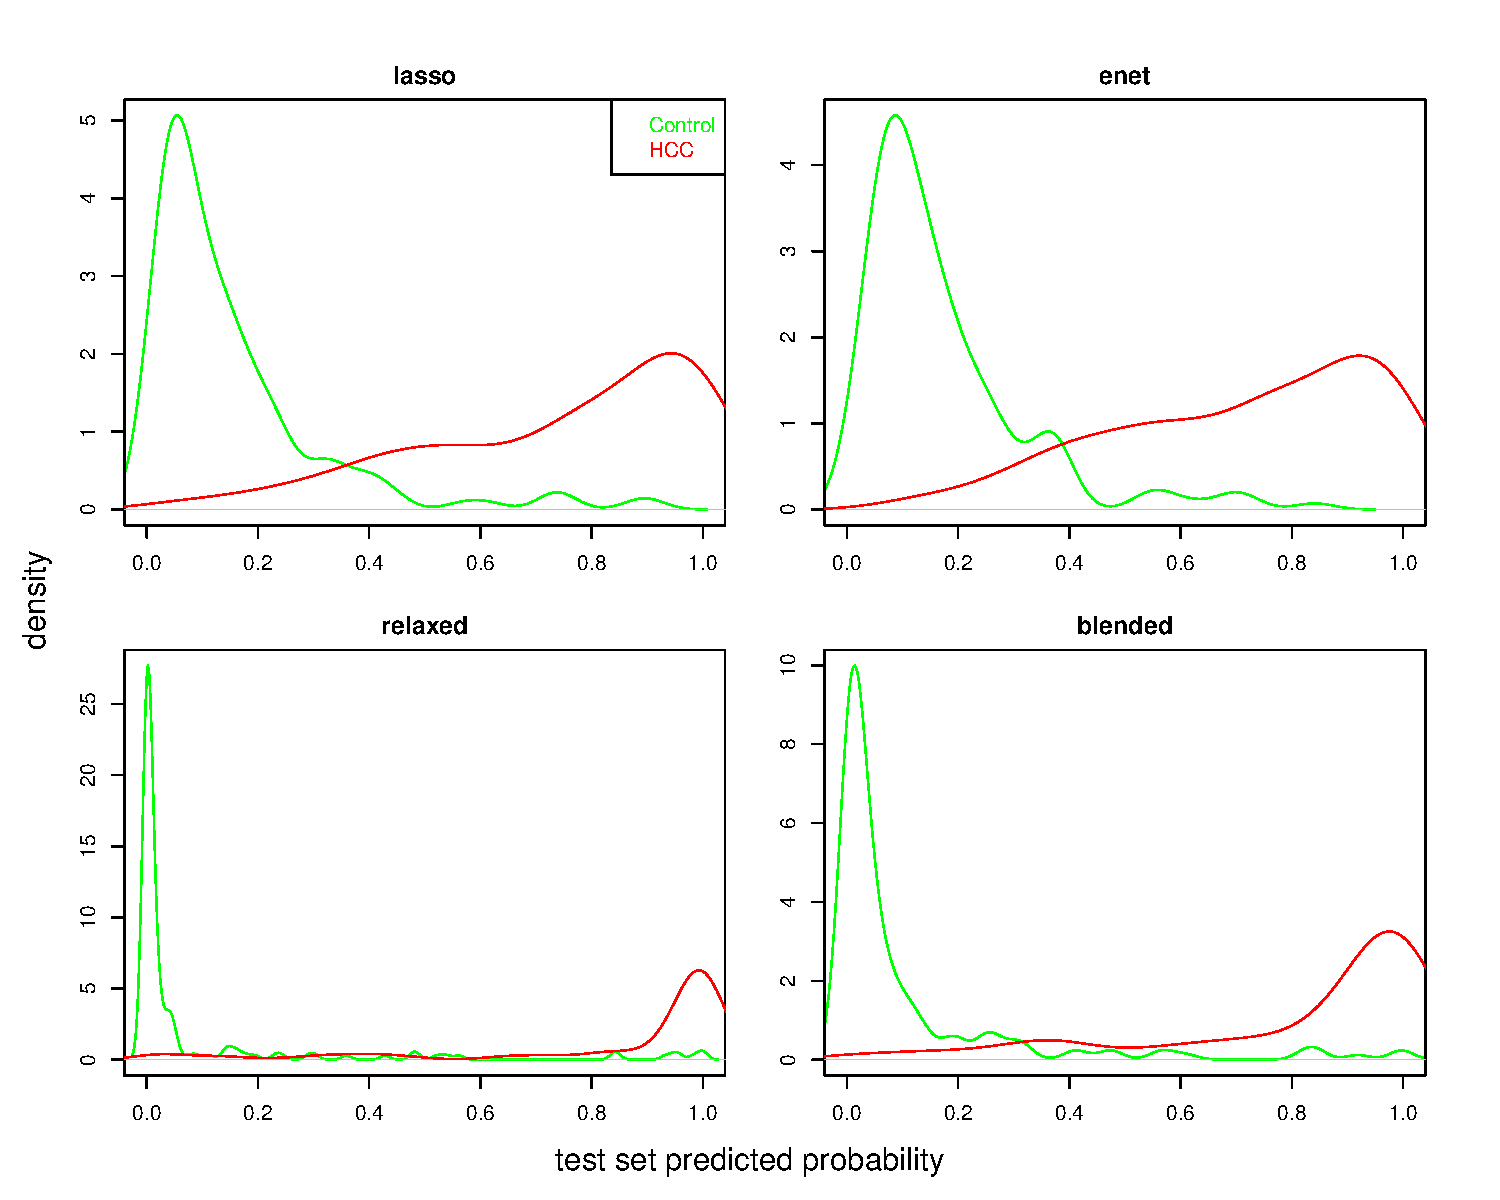
\includegraphics{Static/figures/testOOFprobs-1.pdf}
\caption{\label{fig:testOOFprobs}Test data out-of-fold predicted probabilities}
\end{figure}

\begin{Shaded}
\begin{Highlighting}[]
\CommentTok{\# Define plotting function}
\NormalTok{bxpPredProb\_f <{-}}\StringTok{ }\ControlFlowTok{function}\NormalTok{(cv\_fit, }\DataTypeTok{Gamma=}\OtherTok{NULL}\NormalTok{) \{}
  \CommentTok{\# Train {-} preval is out{-}of{-}fold linear predictor for training design points}
\NormalTok{  onese\_ndx <{-}}\StringTok{ }\KeywordTok{match}\NormalTok{(cv\_fit}\OperatorTok{$}\NormalTok{lambda}\FloatTok{.1}\NormalTok{se, cv\_fit}\OperatorTok{$}\NormalTok{lambda)}
  \ControlFlowTok{if}\NormalTok{(}\KeywordTok{is.null}\NormalTok{(Gamma)) }
\NormalTok{   train\_1se\_preval\_vec <{-}}\StringTok{ }\NormalTok{cv\_fit}\OperatorTok{$}\NormalTok{fit.preval[, onese\_ndx] }\ControlFlowTok{else}
\NormalTok{   train\_1se\_preval\_vec <{-}}\StringTok{ }\NormalTok{cv\_fit}\OperatorTok{$}\NormalTok{fit.preval[[Gamma]][, onese\_ndx] }

\NormalTok{  train\_1se\_predProb\_vec <{-}}\StringTok{ }\KeywordTok{logistic\_f}\NormalTok{(train\_1se\_preval\_vec)}

  \CommentTok{\# Test}
\NormalTok{  test\_1se\_predProb\_vec <{-}}\StringTok{ }\KeywordTok{predict}\NormalTok{(}
\NormalTok{    cv\_fit,}
    \DataTypeTok{newx =}\NormalTok{ test\_lcpm\_mtx,}
    \DataTypeTok{s =} \StringTok{"lambda.1se"}\NormalTok{,}
    \DataTypeTok{type =} \StringTok{"resp"}
\NormalTok{  )}

\NormalTok{  tmp <{-}}\StringTok{ }\KeywordTok{c}\NormalTok{(}
    \DataTypeTok{train =} \KeywordTok{split}\NormalTok{(train\_1se\_predProb\_vec, train\_group\_vec),}
    \DataTypeTok{test =} \KeywordTok{split}\NormalTok{(test\_1se\_predProb\_vec, test\_group\_vec)}
\NormalTok{  )}
  \KeywordTok{names}\NormalTok{(tmp) <{-}}\StringTok{ }\KeywordTok{paste0}\NormalTok{(}\StringTok{"}\CharTok{\textbackslash{}n}\StringTok{"}\NormalTok{, }\KeywordTok{sub}\NormalTok{(}\StringTok{"}\CharTok{\textbackslash{}\textbackslash{}}\StringTok{."}\NormalTok{, }\StringTok{"}\CharTok{\textbackslash{}n}\StringTok{"}\NormalTok{, }\KeywordTok{names}\NormalTok{(tmp)))}

  \KeywordTok{boxplot}\NormalTok{(tmp)}
\NormalTok{\}}

\KeywordTok{par}\NormalTok{(}\DataTypeTok{mfrow =} \KeywordTok{c}\NormalTok{(}\DecValTok{2}\NormalTok{, }\DecValTok{2}\NormalTok{), }\DataTypeTok{mar =} \KeywordTok{c}\NormalTok{(}\DecValTok{5}\NormalTok{, }\DecValTok{3}\NormalTok{, }\DecValTok{2}\NormalTok{, }\DecValTok{1}\NormalTok{), }\DataTypeTok{oma =} \KeywordTok{c}\NormalTok{(}\DecValTok{2}\NormalTok{, }\DecValTok{2}\NormalTok{, }\DecValTok{2}\NormalTok{, }\DecValTok{2}\NormalTok{))}

\KeywordTok{bxpPredProb\_f}\NormalTok{(cv\_lasso)}
\KeywordTok{title}\NormalTok{(}\StringTok{\textquotesingle{}lasso\textquotesingle{}}\NormalTok{)}

\KeywordTok{bxpPredProb\_f}\NormalTok{(cv\_enet)}
\KeywordTok{title}\NormalTok{(}\StringTok{\textquotesingle{}enet\textquotesingle{}}\NormalTok{)}

\KeywordTok{bxpPredProb\_f}\NormalTok{(cv\_lassoR, }\DataTypeTok{Gamma=}\StringTok{\textquotesingle{}g:0\textquotesingle{}}\NormalTok{)}
\KeywordTok{title}\NormalTok{(}\StringTok{\textquotesingle{}relaxed\textquotesingle{}}\NormalTok{)}

\KeywordTok{bxpPredProb\_f}\NormalTok{(cv\_lassoR, }\DataTypeTok{Gamma=}\StringTok{\textquotesingle{}g:0.5\textquotesingle{}}\NormalTok{)}
\KeywordTok{title}\NormalTok{(}\StringTok{\textquotesingle{}blended\textquotesingle{}}\NormalTok{)}
\end{Highlighting}
\end{Shaded}

\begin{figure}
\centering
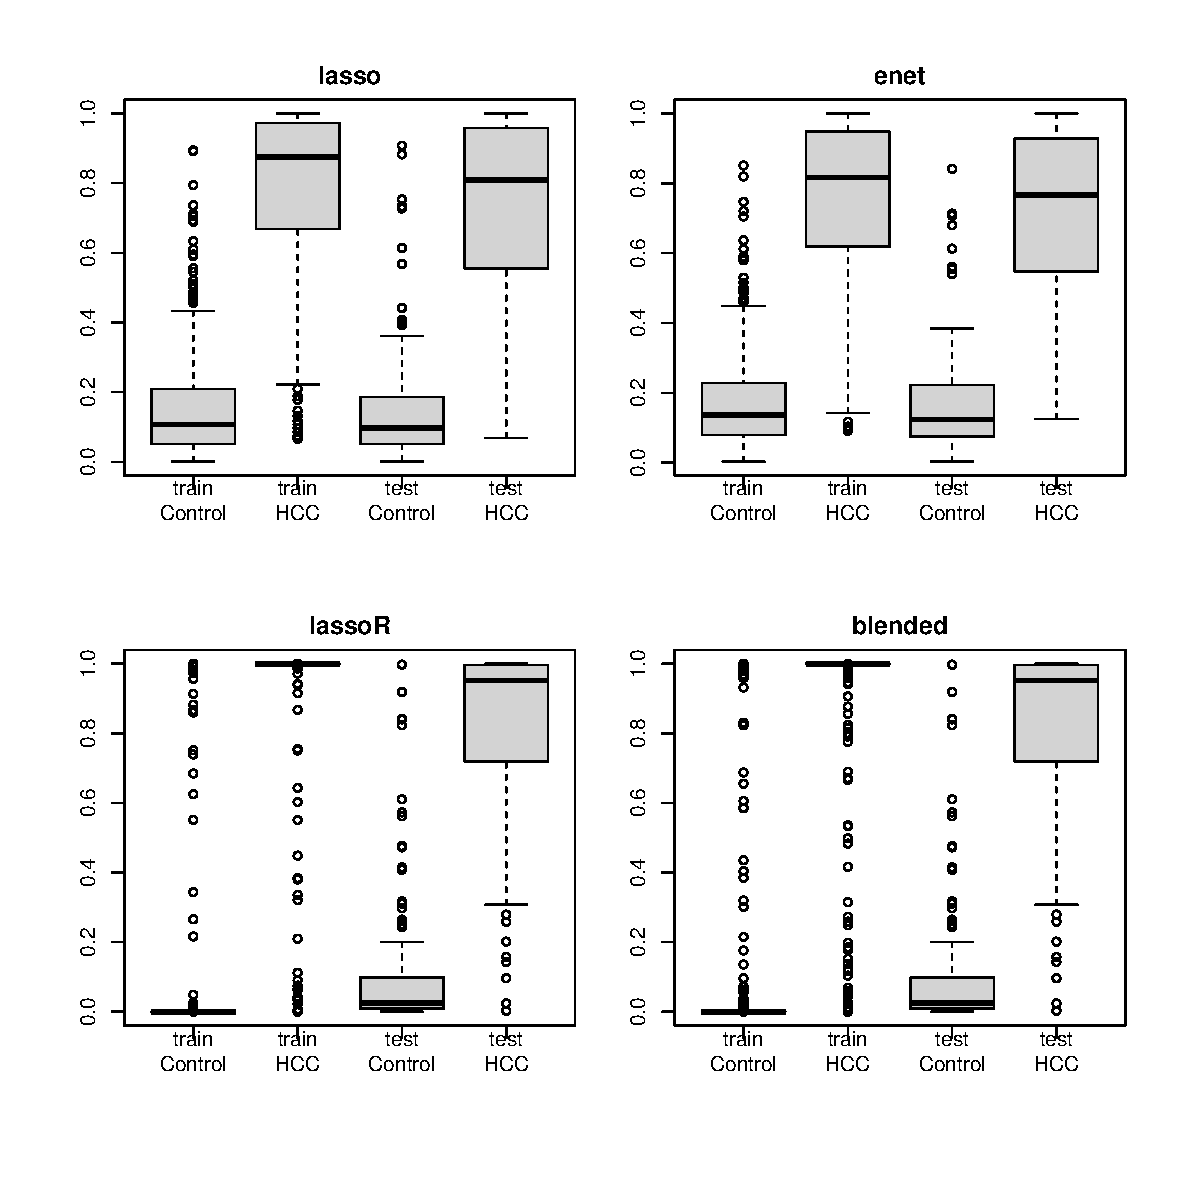
\includegraphics{Static/figures/fitPrevalByGroup-1.pdf}
\caption{\label{fig:fitPrevalByGroup}Predicted Probabilities - Train and Test}
\end{figure}

\hypertarget{compare-predictions-at-misclassified-samples}{%
\section{Compare predictions at misclassified samples}\label{compare-predictions-at-misclassified-samples}}

It is useful to examine classification errors more carefully.
If models have different failure modes, one might get improved
performance by combining model predictions. Note that the models
considered here are not expected to compliment each other usefully
as they are too similar in nature.

\begin{Shaded}
\begin{Highlighting}[]
\CommentTok{\# }\AlertTok{NOTE}\CommentTok{: here we use computred oofClass rather than predClass }
\CommentTok{\# as predClass extracted from predict() are fitted values.}

\CommentTok{\# train {-} oof}
\NormalTok{ndx\_1se <{-}}\StringTok{ }\KeywordTok{match}\NormalTok{(cv\_lasso}\OperatorTok{$}\NormalTok{lambda}\FloatTok{.1}\NormalTok{se,cv\_lasso}\OperatorTok{$}\NormalTok{lambda)}
\NormalTok{train\_lasso\_oofProb\_vec <{-}}\StringTok{ }\KeywordTok{logistic\_f}\NormalTok{(cv\_lasso}\OperatorTok{$}\NormalTok{fit.preval[,ndx\_1se])}
\NormalTok{train\_lasso\_oofClass\_vec <{-}}\StringTok{ }\KeywordTok{ifelse}\NormalTok{(}
\NormalTok{   train\_lasso\_oofProb\_vec }\OperatorTok{>}\StringTok{ }\FloatTok{0.5}\NormalTok{, }\StringTok{\textquotesingle{}HCC\textquotesingle{}}\NormalTok{, }\StringTok{\textquotesingle{}Control\textquotesingle{}}\NormalTok{)}

\NormalTok{ndx\_1se <{-}}\StringTok{ }\KeywordTok{match}\NormalTok{(cv\_enet}\OperatorTok{$}\NormalTok{lambda}\FloatTok{.1}\NormalTok{se,cv\_enet}\OperatorTok{$}\NormalTok{lambda)}
\NormalTok{train\_enet\_oofProb\_vec <{-}}\StringTok{ }\KeywordTok{logistic\_f}\NormalTok{(cv\_enet}\OperatorTok{$}\NormalTok{fit.preval[,ndx\_1se])}
\NormalTok{train\_enet\_oofClass\_vec <{-}}\StringTok{ }\KeywordTok{ifelse}\NormalTok{(}
\NormalTok{   train\_enet\_oofProb\_vec }\OperatorTok{>}\StringTok{ }\FloatTok{0.5}\NormalTok{, }\StringTok{\textquotesingle{}HCC\textquotesingle{}}\NormalTok{, }\StringTok{\textquotesingle{}Control\textquotesingle{}}\NormalTok{)}

\CommentTok{\# RECALL: cv\_lassoR$nzero[cv\_lassoR$lambda==cv\_lassoR$lambda.1se]}
\CommentTok{\# train {-} oof}
\NormalTok{ndx\_1se <{-}}\StringTok{ }\KeywordTok{match}\NormalTok{(cv\_lassoR}\OperatorTok{$}\NormalTok{lambda}\FloatTok{.1}\NormalTok{se,cv\_lassoR}\OperatorTok{$}\NormalTok{lambda)}
\NormalTok{train\_relaxed\_oofProb\_vec <{-}}\StringTok{ }\KeywordTok{logistic\_f}\NormalTok{(cv\_lassoR}\OperatorTok{$}\NormalTok{fit.preval[[}\StringTok{\textquotesingle{}g:0\textquotesingle{}}\NormalTok{]][,ndx\_1se])}
\NormalTok{train\_relaxed\_oofClass\_vec <{-}}\StringTok{ }\KeywordTok{ifelse}\NormalTok{(}
\NormalTok{   train\_relaxed\_oofProb\_vec }\OperatorTok{>}\StringTok{ }\FloatTok{0.5}\NormalTok{, }\StringTok{\textquotesingle{}HCC\textquotesingle{}}\NormalTok{, }\StringTok{\textquotesingle{}Control\textquotesingle{}}\NormalTok{)}

\CommentTok{\# RECALL $\textasciigrave{}r cv\_lassoR$relaxed$nzero.1se\textasciigrave{}$ features (vertical}
\CommentTok{\#  cv\_blended\_statlist <{-} cv\_lassoR$relaxed$statlist[[\textquotesingle{}g:0.5\textquotesingle{}]]}
\CommentTok{\#  cv\_blended\_1se\_error <{-} cv\_blended\_statlist$cvm[cv\_blended\_statlist$lambda==}
      \CommentTok{\#cv\_lassoR$relaxed$lambda.1se]}

\CommentTok{\# train {-} oof}
\NormalTok{cv\_blended\_statlist <{-}}\StringTok{ }\NormalTok{cv\_lassoR}\OperatorTok{$}\NormalTok{relaxed}\OperatorTok{$}\NormalTok{statlist[[}\StringTok{\textquotesingle{}g:0.5\textquotesingle{}}\NormalTok{]]}
\NormalTok{ndx\_1se <{-}}\StringTok{ }\KeywordTok{match}\NormalTok{(cv\_lassoR}\OperatorTok{$}\NormalTok{relaxed}\OperatorTok{$}\NormalTok{lambda}\FloatTok{.1}\NormalTok{se, cv\_blended\_statlist}\OperatorTok{$}\NormalTok{lambda)}
\NormalTok{train\_blended\_oofProb\_vec <{-}}\StringTok{ }\KeywordTok{logistic\_f}\NormalTok{(cv\_lassoR}\OperatorTok{$}\NormalTok{fit.preval[[}\StringTok{\textquotesingle{}g:0.5\textquotesingle{}}\NormalTok{]][,ndx\_1se])}
\NormalTok{train\_blended\_oofClass\_vec <{-}}\StringTok{ }\KeywordTok{ifelse}\NormalTok{(}
\NormalTok{   train\_blended\_oofProb\_vec }\OperatorTok{>}\StringTok{ }\FloatTok{0.5}\NormalTok{, }\StringTok{\textquotesingle{}HCC\textquotesingle{}}\NormalTok{, }\StringTok{\textquotesingle{}Control\textquotesingle{}}\NormalTok{)}


\NormalTok{misclass\_id\_vec <{-}}\StringTok{ }\KeywordTok{unique}\NormalTok{(}\KeywordTok{c}\NormalTok{(}
 \KeywordTok{names}\NormalTok{(train\_lasso\_oofClass\_vec)[train\_lasso\_oofClass\_vec }\OperatorTok{!=}\StringTok{ }\NormalTok{train\_group\_vec],}
 \KeywordTok{names}\NormalTok{(train\_enet\_oofClass\_vec)[train\_enet\_oofClass\_vec }\OperatorTok{!=}\StringTok{ }\NormalTok{train\_group\_vec],}
 \KeywordTok{names}\NormalTok{(train\_relaxed\_oofClass\_vec)[train\_relaxed\_oofClass\_vec }\OperatorTok{!=}\StringTok{ }\NormalTok{train\_group\_vec],}
 \KeywordTok{names}\NormalTok{(train\_blended\_oofClass\_vec)[train\_blended\_oofClass\_vec }\OperatorTok{!=}\StringTok{ }\NormalTok{train\_group\_vec]}
\NormalTok{ )}
\NormalTok{)}


\NormalTok{missclass\_oofProb\_mtx <{-}}\StringTok{ }\KeywordTok{cbind}\NormalTok{(}
\NormalTok{ train\_lasso\_oofProb\_vec[misclass\_id\_vec],}
\NormalTok{ train\_enet\_oofProb\_vec[misclass\_id\_vec],}
\NormalTok{ train\_relaxed\_oofProb\_vec[misclass\_id\_vec],}
\NormalTok{ train\_blended\_oofProb\_vec[misclass\_id\_vec]}
\NormalTok{)}
\KeywordTok{colnames}\NormalTok{(missclass\_oofProb\_mtx) <{-}}\StringTok{ }\KeywordTok{c}\NormalTok{(}\StringTok{\textquotesingle{}lasso\textquotesingle{}}\NormalTok{,}\StringTok{\textquotesingle{}enet\textquotesingle{}}\NormalTok{, }\StringTok{\textquotesingle{}lassoR\textquotesingle{}}\NormalTok{, }\StringTok{\textquotesingle{}blended\textquotesingle{}}\NormalTok{)}

\NormalTok{row\_med\_vec <{-}}\StringTok{ }\KeywordTok{apply}\NormalTok{(missclass\_oofProb\_mtx, }\DecValTok{1}\NormalTok{, median)}
\NormalTok{missclass\_oofProb\_mtx <{-}}\StringTok{ }\NormalTok{missclass\_oofProb\_mtx[}
  \KeywordTok{order}\NormalTok{(train\_group\_vec[}\KeywordTok{rownames}\NormalTok{(missclass\_oofProb\_mtx)], row\_med\_vec),]}

\KeywordTok{plot}\NormalTok{(}
 \DataTypeTok{x=}\KeywordTok{c}\NormalTok{(}\DecValTok{1}\NormalTok{,}\KeywordTok{nrow}\NormalTok{(missclass\_oofProb\_mtx)), }\DataTypeTok{xlab=}\StringTok{\textquotesingle{}samples\textquotesingle{}}\NormalTok{,}
 \DataTypeTok{y=}\KeywordTok{range}\NormalTok{(missclass\_oofProb\_mtx), }\DataTypeTok{ylab=}\StringTok{\textquotesingle{}out{-}of{-}fold predicted probability\textquotesingle{}}\NormalTok{,}
 \DataTypeTok{xaxt=}\StringTok{\textquotesingle{}n\textquotesingle{}}\NormalTok{, }\DataTypeTok{type=}\StringTok{\textquotesingle{}n\textquotesingle{}}\NormalTok{)}

\ControlFlowTok{for}\NormalTok{(RR }\ControlFlowTok{in} \DecValTok{1}\OperatorTok{:}\KeywordTok{nrow}\NormalTok{(missclass\_oofProb\_mtx))}
\KeywordTok{points}\NormalTok{(}
 \KeywordTok{rep}\NormalTok{(RR, }\KeywordTok{ncol}\NormalTok{(missclass\_oofProb\_mtx)), }
\NormalTok{ missclass\_oofProb\_mtx[RR,],}
 \DataTypeTok{col=}\KeywordTok{ifelse}\NormalTok{(train\_group\_vec[}\KeywordTok{rownames}\NormalTok{(missclass\_oofProb\_mtx)[RR]] }\OperatorTok{==}\StringTok{ \textquotesingle{}Control\textquotesingle{}}\NormalTok{,}
  \StringTok{\textquotesingle{}green\textquotesingle{}}\NormalTok{, }\StringTok{\textquotesingle{}red\textquotesingle{}}\NormalTok{),}
 \DataTypeTok{pch=}\DecValTok{1}\OperatorTok{:}\KeywordTok{ncol}\NormalTok{(missclass\_oofProb\_mtx))}

\KeywordTok{legend}\NormalTok{(}\StringTok{\textquotesingle{}top\textquotesingle{}}\NormalTok{, }\DataTypeTok{ncol=}\DecValTok{2}\NormalTok{, }\DataTypeTok{legend=}\KeywordTok{colnames}\NormalTok{(missclass\_oofProb\_mtx), }
 \DataTypeTok{pch=}\DecValTok{1}\OperatorTok{:}\DecValTok{4}\NormalTok{, }\DataTypeTok{bty=}\StringTok{\textquotesingle{}n\textquotesingle{}}\NormalTok{)}

\KeywordTok{abline}\NormalTok{(}\DataTypeTok{h=}\FloatTok{0.5}\NormalTok{)}
\end{Highlighting}
\end{Shaded}

\begin{figure}
\centering
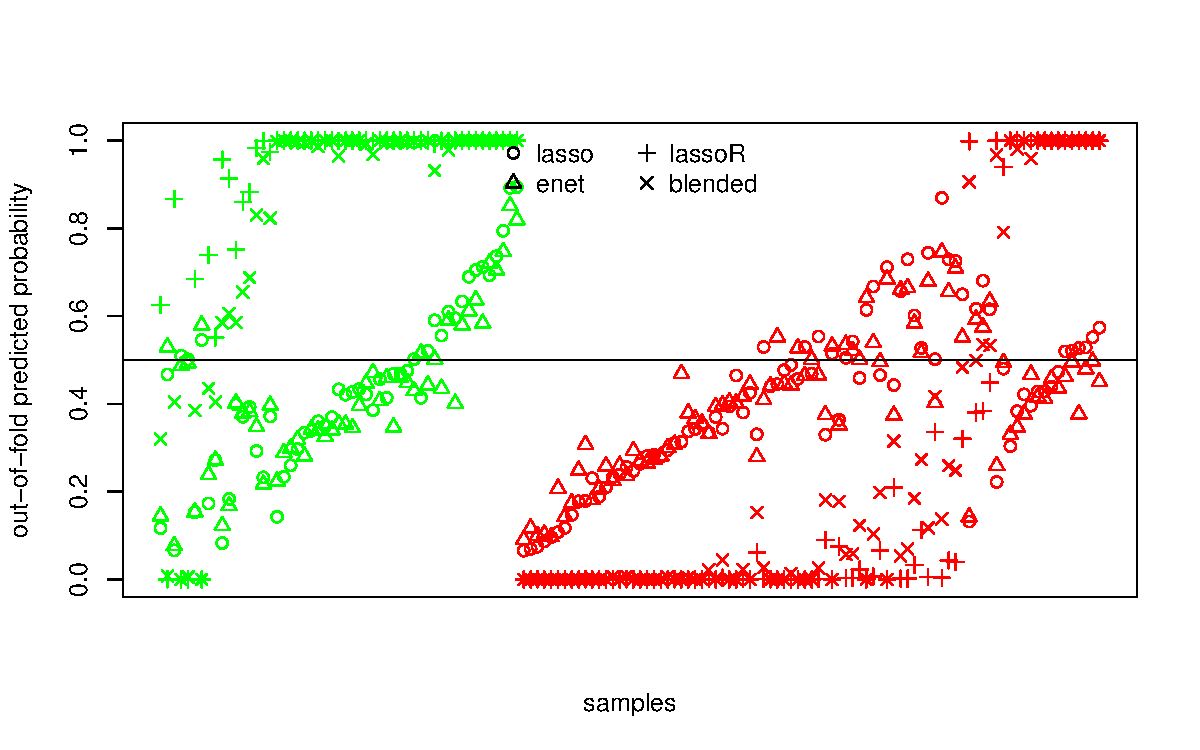
\includegraphics{Static/figures/misclassTrain-1.pdf}
\caption{\label{fig:misclassTrain}out-of-fold predicted probabilities at miscassified samples}
\end{figure}

As we've seen above, predictions from lassoR and the blended mix model
are basically dichotomous; 0 or 1. Samples have been order by group, and
median P(HCC) within group. For the Controls (green), predicted probabilities
less than 0.5 are considered correct here. For the HCC (red) samples,
predicted probabilities greater than 0.5 are considered correct here.

Now look at the same plot on the test data set.

\begin{Shaded}
\begin{Highlighting}[]
\NormalTok{test\_lasso\_predClass\_vec <{-}}\StringTok{ }\KeywordTok{predict}\NormalTok{(}
\NormalTok{ cv\_lasso,}
 \DataTypeTok{newx=}\NormalTok{test\_lcpm\_mtx,}
 \DataTypeTok{s=}\StringTok{\textquotesingle{}lambda.1se\textquotesingle{}}\NormalTok{,}
 \DataTypeTok{type=}\StringTok{\textquotesingle{}class\textquotesingle{}}
\NormalTok{)}

\NormalTok{test\_enet\_predClass\_vec <{-}}\StringTok{ }\KeywordTok{predict}\NormalTok{(}
\NormalTok{ cv\_enet,}
 \DataTypeTok{newx=}\NormalTok{test\_lcpm\_mtx,}
 \DataTypeTok{s=}\StringTok{\textquotesingle{}lambda.1se\textquotesingle{}}\NormalTok{,}
 \DataTypeTok{type=}\StringTok{\textquotesingle{}class\textquotesingle{}}
\NormalTok{)}

\NormalTok{test\_relaxed\_predClass\_vec <{-}}\StringTok{ }\KeywordTok{predict}\NormalTok{(}
\NormalTok{ cv\_lassoR,}
 \DataTypeTok{g=}\DecValTok{0}\NormalTok{,}
 \DataTypeTok{newx=}\NormalTok{test\_lcpm\_mtx,}
 \DataTypeTok{s=}\StringTok{\textquotesingle{}lambda.1se\textquotesingle{}}\NormalTok{,}
 \DataTypeTok{type=}\StringTok{\textquotesingle{}class\textquotesingle{}}
\NormalTok{)}

\NormalTok{test\_blended\_predClass\_vec <{-}}\StringTok{ }\KeywordTok{predict}\NormalTok{(}
\NormalTok{ cv\_lassoR,}
 \DataTypeTok{g=}\FloatTok{0.5}\NormalTok{,}
 \DataTypeTok{newx=}\NormalTok{test\_lcpm\_mtx,}
 \DataTypeTok{s=}\StringTok{\textquotesingle{}lambda.1se\textquotesingle{}}\NormalTok{,}
 \DataTypeTok{type=}\StringTok{\textquotesingle{}class\textquotesingle{}}
\NormalTok{)}

\NormalTok{misclass\_id\_vec <{-}}\StringTok{ }\KeywordTok{unique}\NormalTok{(}\KeywordTok{c}\NormalTok{(}
 \KeywordTok{names}\NormalTok{(test\_lasso\_predClass\_vec[,}\DecValTok{1}\NormalTok{])[test\_lasso\_predClass\_vec }\OperatorTok{!=}\StringTok{ }\NormalTok{test\_group\_vec],}
 \KeywordTok{names}\NormalTok{(test\_enet\_predClass\_vec[,}\DecValTok{1}\NormalTok{])[test\_enet\_predClass\_vec }\OperatorTok{!=}\StringTok{ }\NormalTok{test\_group\_vec],}
 \KeywordTok{names}\NormalTok{(test\_relaxed\_predClass\_vec[,}\DecValTok{1}\NormalTok{])[test\_relaxed\_predClass\_vec }\OperatorTok{!=}\StringTok{ }\NormalTok{test\_group\_vec],}
 \KeywordTok{names}\NormalTok{(test\_blended\_predClass\_vec[,}\DecValTok{1}\NormalTok{])[test\_blended\_predClass\_vec }\OperatorTok{!=}\StringTok{ }\NormalTok{test\_group\_vec]}
\NormalTok{ )}
\NormalTok{)}


\NormalTok{missclass\_oofProb\_mtx <{-}}\StringTok{ }\KeywordTok{cbind}\NormalTok{(}
\NormalTok{ test\_lasso\_predProb\_vec[misclass\_id\_vec,],}
\NormalTok{ test\_enet\_predProb\_vec[misclass\_id\_vec,],}
\NormalTok{ test\_relaxed\_predProb\_vec[misclass\_id\_vec,],}
\NormalTok{ test\_blended\_predProb\_vec[misclass\_id\_vec,]}
\NormalTok{)}
\KeywordTok{colnames}\NormalTok{(missclass\_oofProb\_mtx) <{-}}\StringTok{ }\KeywordTok{c}\NormalTok{(}\StringTok{\textquotesingle{}lasso\textquotesingle{}}\NormalTok{,}\StringTok{\textquotesingle{}enet\textquotesingle{}}\NormalTok{, }\StringTok{\textquotesingle{}lassoR\textquotesingle{}}\NormalTok{, }\StringTok{\textquotesingle{}blended\textquotesingle{}}\NormalTok{)}

\NormalTok{row\_med\_vec <{-}}\StringTok{ }\KeywordTok{apply}\NormalTok{(missclass\_oofProb\_mtx, }\DecValTok{1}\NormalTok{, median)}
\NormalTok{missclass\_oofProb\_mtx <{-}}\StringTok{ }\NormalTok{missclass\_oofProb\_mtx[}
  \KeywordTok{order}\NormalTok{(test\_group\_vec[}\KeywordTok{rownames}\NormalTok{(missclass\_oofProb\_mtx)], row\_med\_vec),]}

\KeywordTok{plot}\NormalTok{(}
 \DataTypeTok{x=}\KeywordTok{c}\NormalTok{(}\DecValTok{1}\NormalTok{,}\KeywordTok{nrow}\NormalTok{(missclass\_oofProb\_mtx)), }\DataTypeTok{xlab=}\StringTok{\textquotesingle{}samples\textquotesingle{}}\NormalTok{,}
 \DataTypeTok{y=}\KeywordTok{range}\NormalTok{(missclass\_oofProb\_mtx), }\DataTypeTok{ylab=}\StringTok{\textquotesingle{}out{-}of{-}fold predicted probability\textquotesingle{}}\NormalTok{,}
 \DataTypeTok{xaxt=}\StringTok{\textquotesingle{}n\textquotesingle{}}\NormalTok{, }\DataTypeTok{type=}\StringTok{\textquotesingle{}n\textquotesingle{}}\NormalTok{)}

\ControlFlowTok{for}\NormalTok{(RR }\ControlFlowTok{in} \DecValTok{1}\OperatorTok{:}\KeywordTok{nrow}\NormalTok{(missclass\_oofProb\_mtx))}
\KeywordTok{points}\NormalTok{(}
 \KeywordTok{rep}\NormalTok{(RR, }\KeywordTok{ncol}\NormalTok{(missclass\_oofProb\_mtx)), }
\NormalTok{ missclass\_oofProb\_mtx[RR,],}
 \DataTypeTok{col=}\KeywordTok{ifelse}\NormalTok{(test\_group\_vec[}\KeywordTok{rownames}\NormalTok{(missclass\_oofProb\_mtx)[RR]] }\OperatorTok{==}\StringTok{ \textquotesingle{}Control\textquotesingle{}}\NormalTok{,}
  \StringTok{\textquotesingle{}green\textquotesingle{}}\NormalTok{, }\StringTok{\textquotesingle{}red\textquotesingle{}}\NormalTok{),}
 \DataTypeTok{pch=}\DecValTok{1}\OperatorTok{:}\KeywordTok{ncol}\NormalTok{(missclass\_oofProb\_mtx))}

\KeywordTok{legend}\NormalTok{(}\StringTok{\textquotesingle{}top\textquotesingle{}}\NormalTok{, }\DataTypeTok{ncol=}\DecValTok{2}\NormalTok{, }\DataTypeTok{legend=}\KeywordTok{colnames}\NormalTok{(missclass\_oofProb\_mtx), }
 \DataTypeTok{pch=}\DecValTok{1}\OperatorTok{:}\DecValTok{4}\NormalTok{, }\DataTypeTok{bty=}\StringTok{\textquotesingle{}n\textquotesingle{}}\NormalTok{)}

\KeywordTok{abline}\NormalTok{(}\DataTypeTok{h=}\FloatTok{0.5}\NormalTok{)}
\end{Highlighting}
\end{Shaded}

\begin{figure}
\centering
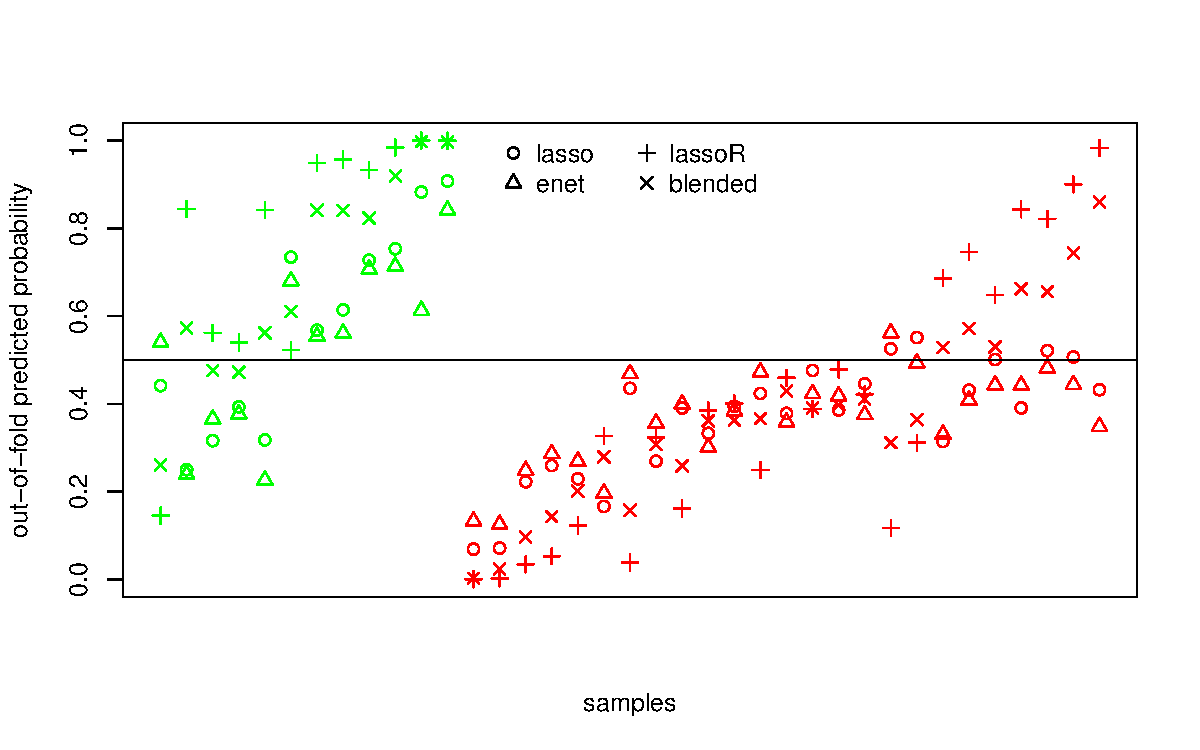
\includegraphics{Static/figures/misclassTest-1.pdf}
\caption{\label{fig:misclassTest}Test data predicted probabilities at miscassified samples}
\end{figure}

The relaxed lasso fit results in essentially dichotomized predicted probability
distribution - predicted probabilities are very close to 0 or 1.

We see that for design points in the training set, the predicted probabilies from the relaxed lasso
are essentially dichotomized to be tightly distributed at the extremes of the
response range. For design points in the test set, the predicted probabilies from the relaxed lasso
are comparable to the lasso model predicted porbabilities. This seems to indicate over-fitting
in the relaxed lasso fit.

\hypertarget{compare-coefficient-profiles}{%
\section{Compare coefficient profiles}\label{compare-coefficient-profiles}}

\begin{Shaded}
\begin{Highlighting}[]
\CommentTok{\# lasso }
\CommentTok{\#\#\#\#\#\#\#\#\#\#\#\#\#\#\#\#\#\#\#\#\#\#\#\#\#\#}
\CommentTok{\# train {-} cv predicted}
\NormalTok{lasso\_coef <{-}}\StringTok{ }\KeywordTok{coef}\NormalTok{(}
\NormalTok{ cv\_lasso,}
 \DataTypeTok{s=}\StringTok{\textquotesingle{}lambda.1se\textquotesingle{}}
\NormalTok{)}
\NormalTok{lasso\_coef\_frm <{-}}\StringTok{ }\KeywordTok{data.frame}\NormalTok{(}
 \DataTypeTok{gene=}\NormalTok{lasso\_coef}\OperatorTok{@}\NormalTok{Dimnames[[}\DecValTok{1}\NormalTok{]][}\KeywordTok{c}\NormalTok{(}\DecValTok{1}\NormalTok{, lasso\_coef}\OperatorTok{@}\NormalTok{i[}\OperatorTok{{-}}\DecValTok{1}\NormalTok{])],}
 \DataTypeTok{lasso=}\NormalTok{lasso\_coef}\OperatorTok{@}\NormalTok{x)}


\CommentTok{\# enet}
\CommentTok{\#\#\#\#\#\#\#\#\#\#\#\#\#\#\#\#\#\#\#\#\#\#\#\#\#\#}
\NormalTok{enet\_coef <{-}}\StringTok{ }\KeywordTok{coef}\NormalTok{(}
\NormalTok{ cv\_enet,}
 \DataTypeTok{s=}\StringTok{\textquotesingle{}lambda.1se\textquotesingle{}}
\NormalTok{)}
\NormalTok{enet\_coef\_frm <{-}}\StringTok{ }\KeywordTok{data.frame}\NormalTok{(}
 \DataTypeTok{gene=}\NormalTok{enet\_coef}\OperatorTok{@}\NormalTok{Dimnames[[}\DecValTok{1}\NormalTok{]][}\KeywordTok{c}\NormalTok{(}\DecValTok{1}\NormalTok{, enet\_coef}\OperatorTok{@}\NormalTok{i[}\OperatorTok{{-}}\DecValTok{1}\NormalTok{])],}
 \DataTypeTok{enet=}\NormalTok{enet\_coef}\OperatorTok{@}\NormalTok{x)}

\CommentTok{\# THESE ARE NOT CORRECT {-} SKIP}
\CommentTok{\# relaxed lasso (gamma=0)}
\CommentTok{\#\#\#\#\#\#\#\#\#\#\#\#\#\#\#\#\#\#\#\#\#\#\#\#\#\#}
\NormalTok{SKIP <{-}}\StringTok{ }\ControlFlowTok{function}\NormalTok{() \{}
\NormalTok{lassoR\_coef <{-}}\StringTok{ }\KeywordTok{coef}\NormalTok{(}
\NormalTok{ cv\_lassoR,}
 \DataTypeTok{s=}\StringTok{\textquotesingle{}lambda.1se\textquotesingle{}}\NormalTok{,}
 \DataTypeTok{g=}\DecValTok{0}
\NormalTok{)}
\NormalTok{lassoR\_coef\_frm <{-}}\StringTok{ }\KeywordTok{data.frame}\NormalTok{(}
 \DataTypeTok{gene=}\NormalTok{lassoR\_coef}\OperatorTok{@}\NormalTok{Dimnames[[}\DecValTok{1}\NormalTok{]][}\KeywordTok{c}\NormalTok{(}\DecValTok{1}\NormalTok{, lassoR\_coef}\OperatorTok{@}\NormalTok{i[}\OperatorTok{{-}}\DecValTok{1}\NormalTok{])],}
 \DataTypeTok{lassoR=}\NormalTok{lassoR\_coef}\OperatorTok{@}\NormalTok{x)}
\NormalTok{\}}

\CommentTok{\# blended mix (gamma=0.5)}
\CommentTok{\#\#\#\#\#\#\#\#\#\#\#\#\#\#\#\#\#\#\#\#\#\#\#\#\#\#\#\#\#\#\#}
\NormalTok{blended\_coef <{-}}\StringTok{ }\KeywordTok{coef}\NormalTok{(}
\NormalTok{ cv\_lassoR,}
 \DataTypeTok{s=}\StringTok{\textquotesingle{}lambda.1se\textquotesingle{}}\NormalTok{,}
 \DataTypeTok{g=}\FloatTok{0.5}
\NormalTok{)}
\NormalTok{blended\_coef\_frm <{-}}\StringTok{ }\KeywordTok{data.frame}\NormalTok{(}
 \DataTypeTok{gene=}\NormalTok{blended\_coef}\OperatorTok{@}\NormalTok{Dimnames[[}\DecValTok{1}\NormalTok{]][}\KeywordTok{c}\NormalTok{(}\DecValTok{1}\NormalTok{, blended\_coef}\OperatorTok{@}\NormalTok{i[}\OperatorTok{{-}}\DecValTok{1}\NormalTok{])],}
 \DataTypeTok{blended=}\NormalTok{blended\_coef}\OperatorTok{@}\NormalTok{x)}


\CommentTok{\# put it all together}
\NormalTok{all\_coef\_frm <{-}}\StringTok{ }
\StringTok{ }\NormalTok{base}\OperatorTok{::}\KeywordTok{merge}\NormalTok{(}
 \DataTypeTok{x =}\NormalTok{ lasso\_coef\_frm, }
 \DataTypeTok{y =}\NormalTok{ base}\OperatorTok{::}\KeywordTok{merge}\NormalTok{(}
     \DataTypeTok{x =}\NormalTok{ enet\_coef\_frm,}
     \DataTypeTok{y =}\NormalTok{ blended\_coef\_frm,}
         \DataTypeTok{by=}\StringTok{\textquotesingle{}gene\textquotesingle{}}\NormalTok{, }\DataTypeTok{all=}\NormalTok{T),}
 \DataTypeTok{by=}\StringTok{\textquotesingle{}gene\textquotesingle{}}\NormalTok{, }\DataTypeTok{all=}\NormalTok{T)}

\CommentTok{\# SKIPPED}
\CommentTok{\#base::merge(}
         \CommentTok{\#x = lassoR\_coef\_frm,}
         \CommentTok{\#y = blended\_coef\_frm,}
         \CommentTok{\#by=\textquotesingle{}gene\textquotesingle{}, all=T),}

\NormalTok{all\_coef\_frm[,}\OperatorTok{{-}}\DecValTok{1}\NormalTok{][}\KeywordTok{is.na}\NormalTok{(all\_coef\_frm[,}\OperatorTok{{-}}\DecValTok{1}\NormalTok{])] <{-}}\StringTok{ }\DecValTok{0}

\KeywordTok{par}\NormalTok{(}\DataTypeTok{mfrow=}\KeywordTok{c}\NormalTok{(}\KeywordTok{ncol}\NormalTok{(all\_coef\_frm)}\OperatorTok{{-}}\DecValTok{1}\NormalTok{,}\DecValTok{1}\NormalTok{), }\DataTypeTok{mar=}\KeywordTok{c}\NormalTok{(}\DecValTok{0}\NormalTok{,}\DecValTok{5}\NormalTok{,}\DecValTok{0}\NormalTok{,}\DecValTok{1}\NormalTok{), }\DataTypeTok{oma=}\KeywordTok{c}\NormalTok{(}\DecValTok{3}\NormalTok{,}\DecValTok{1}\NormalTok{,}\DecValTok{2}\NormalTok{,}\DecValTok{0}\NormalTok{))}

\ControlFlowTok{for}\NormalTok{(CC }\ControlFlowTok{in} \DecValTok{2}\OperatorTok{:}\KeywordTok{ncol}\NormalTok{(all\_coef\_frm)) \{}
 \KeywordTok{plot}\NormalTok{(}
  \DataTypeTok{x=}\DecValTok{1}\OperatorTok{:}\NormalTok{(}\KeywordTok{nrow}\NormalTok{(all\_coef\_frm)}\OperatorTok{{-}}\DecValTok{1}\NormalTok{), }\DataTypeTok{xlab=}\StringTok{\textquotesingle{}\textquotesingle{}}\NormalTok{, }
  \DataTypeTok{y=}\NormalTok{all\_coef\_frm[}\OperatorTok{{-}}\DecValTok{1}\NormalTok{, CC], }\DataTypeTok{ylab=}\KeywordTok{colnames}\NormalTok{(all\_coef\_frm)[CC],}
  \DataTypeTok{type=}\StringTok{\textquotesingle{}h\textquotesingle{}}\NormalTok{, }\DataTypeTok{xaxt=}\StringTok{\textquotesingle{}n\textquotesingle{}}\NormalTok{)}
\NormalTok{\}}
\end{Highlighting}
\end{Shaded}

\begin{figure}
\centering
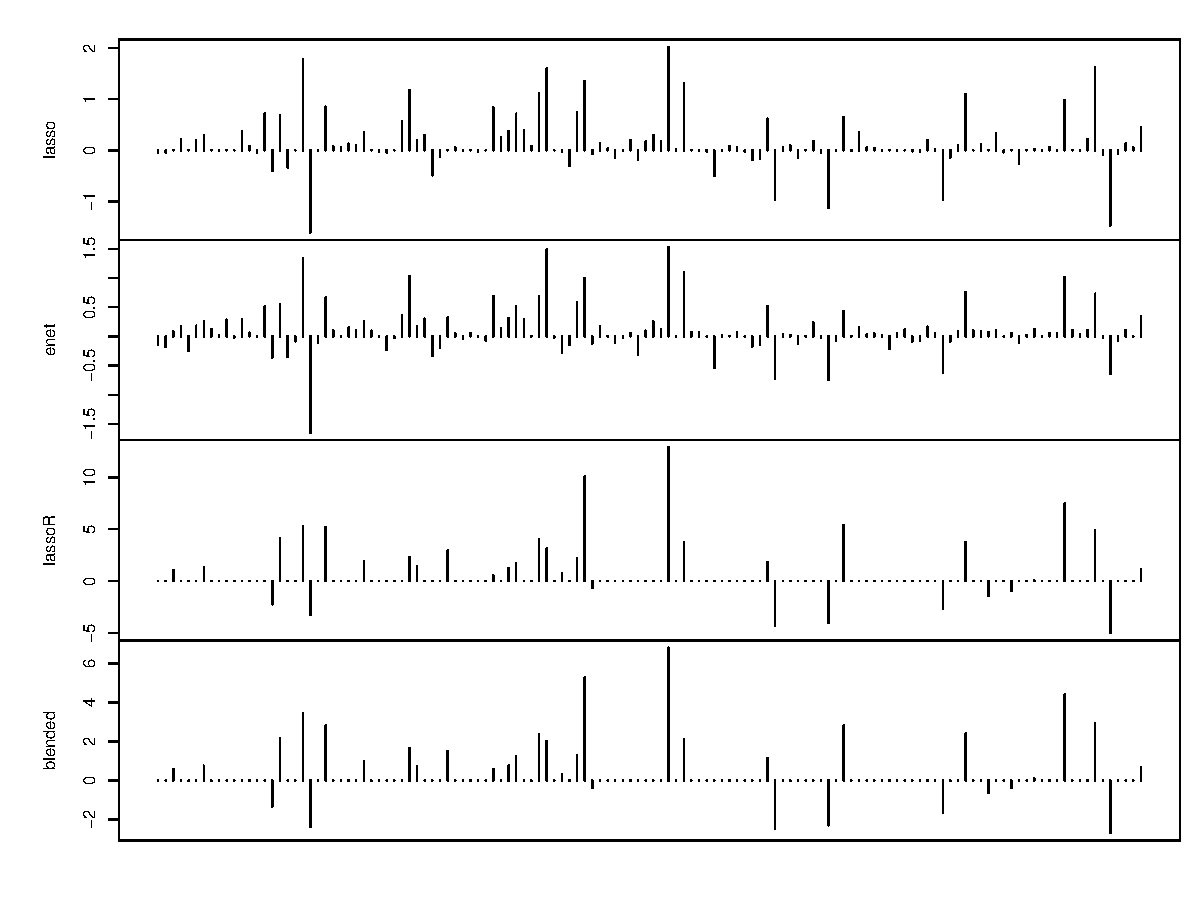
\includegraphics{Static/figures/compCoeffProf-1.pdf}
\caption{\label{fig:compCoeffProf}Coefficient Profiles}
\end{figure}

Note that there is little difference between the elastic net and the lasso
in the selected features, and when the coefficient is zero in one set, it
is smaell in the other. By contrast, the blended fit produces more shrinkage.

\begin{Shaded}
\begin{Highlighting}[]
\NormalTok{knitr}\OperatorTok{::}\KeywordTok{kable}\NormalTok{(}
\KeywordTok{with}\NormalTok{(all\_coef\_frm[,}\OperatorTok{{-}}\DecValTok{1}\NormalTok{], }\KeywordTok{table}\NormalTok{(}\DataTypeTok{lassoZero=}\NormalTok{lasso}\OperatorTok{==}\DecValTok{0}\NormalTok{, }\DataTypeTok{enetZero=}\NormalTok{enet}\OperatorTok{==}\DecValTok{0}\NormalTok{)),}
 \DataTypeTok{caption=}\StringTok{\textquotesingle{}Zero Ceofficient: rows are lasso, columns enet\textquotesingle{}}\NormalTok{) }\OperatorTok{\%>\%}
\StringTok{  }\NormalTok{kableExtra}\OperatorTok{::}\KeywordTok{kable\_styling}\NormalTok{(}\DataTypeTok{full\_width =}\NormalTok{ F)}
\end{Highlighting}
\end{Shaded}

\begin{table}

\caption{\label{tab:zreros}Zero Ceofficient: rows are lasso, columns enet}
\centering
\begin{tabular}[t]{l|r|r}
\hline
  & FALSE & TRUE\\
\hline
FALSE & 88 & 12\\
\hline
TRUE & 31 & 0\\
\hline
\end{tabular}
\end{table}

Coefficients in the blended fit are larger than those in the
lasso fit, or zero.

We can also examine these with a scatter plot matrix.

\begin{Shaded}
\begin{Highlighting}[]
\KeywordTok{pairs}\NormalTok{(all\_coef\_frm[}\OperatorTok{{-}}\DecValTok{1}\NormalTok{,}\OperatorTok{{-}}\DecValTok{1}\NormalTok{],}
  \DataTypeTok{lower.panel =} \OtherTok{NULL}\NormalTok{,}
  \DataTypeTok{panel =} \ControlFlowTok{function}\NormalTok{(x, y) \{}
    \KeywordTok{points}\NormalTok{(x, y, }\DataTypeTok{pch =} \DecValTok{16}\NormalTok{, }\DataTypeTok{col =} \StringTok{"blue"}\NormalTok{)}
\NormalTok{  \}}
\NormalTok{)}
\end{Highlighting}
\end{Shaded}

\begin{figure}
\centering
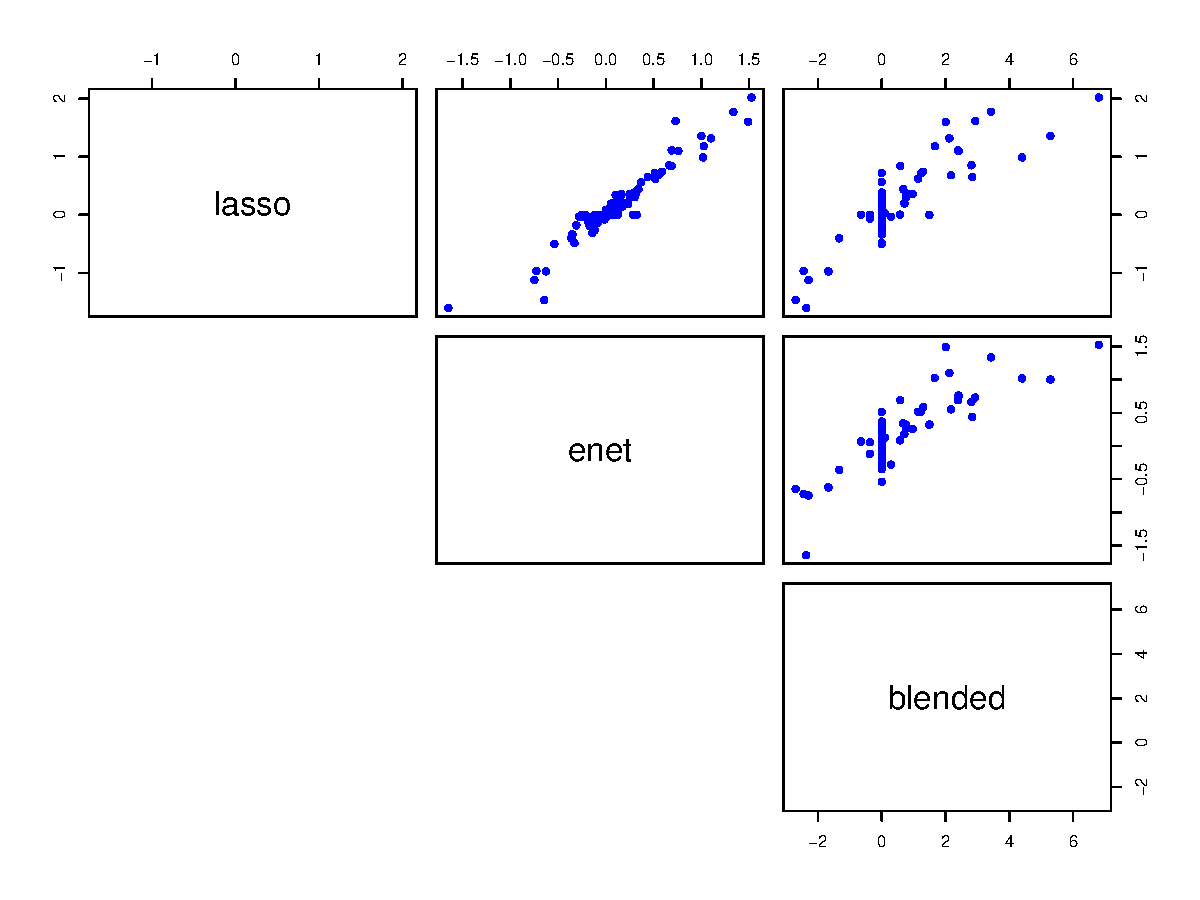
\includegraphics{Static/figures/pairsCoeffProf-1.pdf}
\caption{\label{fig:pairsCoeffProf}Coefficients from fits}
\end{figure}

\hypertarget{examine-feature-selection}{%
\section{Examine feature selection}\label{examine-feature-selection}}

Recall from \texttt{glmnet} vignette:

\begin{verbatim}
It is known that the ridge penalty shrinks the coefficients of correlated predictors
towards each other while the lasso tends to pick one of them and discard the others.
The elastic-net penalty mixes these two; if predictors are correlated in groups,
an $\alpha$=0.5 tends to select the groups in or out together.
This is a higher level parameter, and users might pick a value upfront,
else experiment with a few different values. One use of $\alpha$ is for numerical stability;
for example, the *elastic net with $\alpha = 1 - \epsilon$ for some small $\epsilon$>0
performs much like the lasso, but removes any degeneracies and wild behavior caused
by extreme correlations*.
\end{verbatim}

To see how this plays out in this dataset, we can look at feature expression
heat maps.

Reader notes:

\begin{verbatim}
Heat maps are rarely useful other than to display the obvious.
Here too heat maps fail to yield any insights, or confirmation
of the relationship between feature correlation and lasso vs enet
feature selection.
\end{verbatim}

\begin{Shaded}
\begin{Highlighting}[]
 \KeywordTok{suppressPackageStartupMessages}\NormalTok{(}\KeywordTok{require}\NormalTok{(gplots))}

\CommentTok{\# train {-} cv predicted}
\NormalTok{lasso\_coef <{-}}\StringTok{ }\KeywordTok{coef}\NormalTok{(}
\NormalTok{ cv\_lasso,}
 \DataTypeTok{s=}\StringTok{\textquotesingle{}lambda.1se\textquotesingle{}}
\NormalTok{)}
\NormalTok{lasso\_coef\_frm <{-}}\StringTok{ }\KeywordTok{data.frame}\NormalTok{(}
 \DataTypeTok{gene=}\NormalTok{lasso\_coef}\OperatorTok{@}\NormalTok{Dimnames[[}\DecValTok{1}\NormalTok{]][}\KeywordTok{c}\NormalTok{(}\DecValTok{1}\NormalTok{, lasso\_coef}\OperatorTok{@}\NormalTok{i[}\OperatorTok{{-}}\DecValTok{1}\NormalTok{])],}
 \DataTypeTok{lasso=}\NormalTok{lasso\_coef}\OperatorTok{@}\NormalTok{x)}

 
\NormalTok{  Mycol <{-}}\StringTok{ }\KeywordTok{colorpanel}\NormalTok{(}\DecValTok{1000}\NormalTok{, }\StringTok{"blue"}\NormalTok{, }\StringTok{"red"}\NormalTok{)}
  \KeywordTok{heatmap.2}\NormalTok{(}
    \DataTypeTok{x=}\KeywordTok{t}\NormalTok{(train\_lcpm\_mtx[,lasso\_coef\_frm}\OperatorTok{$}\NormalTok{gene[}\OperatorTok{{-}}\DecValTok{1}\NormalTok{]]),}
    \DataTypeTok{scale=}\StringTok{"row"}\NormalTok{,}
    \DataTypeTok{labRow=}\NormalTok{lasso\_coef\_frm}\OperatorTok{$}\NormalTok{gene,}
    \DataTypeTok{labCol=}\NormalTok{train\_group\_vec,}
    \DataTypeTok{col=}\NormalTok{Mycol, }
    \DataTypeTok{trace=}\StringTok{"none"}\NormalTok{, }\DataTypeTok{density.info=}\StringTok{"none"}\NormalTok{, }
    \CommentTok{\#margin=c(8,6), lhei=c(2,10), }
    \CommentTok{\#lwid=c(0.1,4), \#lhei=c(0.1,4)}
    \DataTypeTok{key=}\NormalTok{F,}
    \DataTypeTok{ColSideColors=}\KeywordTok{ifelse}\NormalTok{(train\_group\_vec}\OperatorTok{==}\StringTok{\textquotesingle{}Control\textquotesingle{}}\NormalTok{, }\StringTok{\textquotesingle{}green\textquotesingle{}}\NormalTok{,}\StringTok{\textquotesingle{}red\textquotesingle{}}\NormalTok{),}
    \DataTypeTok{dendrogram=}\StringTok{"both"}\NormalTok{,}
    \DataTypeTok{main=}\KeywordTok{paste}\NormalTok{(}\StringTok{\textquotesingle{}lasso genes {-} N =\textquotesingle{}}\NormalTok{, }\KeywordTok{nrow}\NormalTok{(lasso\_coef\_frm)}\OperatorTok{{-}}\DecValTok{1}\NormalTok{))}
\end{Highlighting}
\end{Shaded}

\begin{figure}
\centering
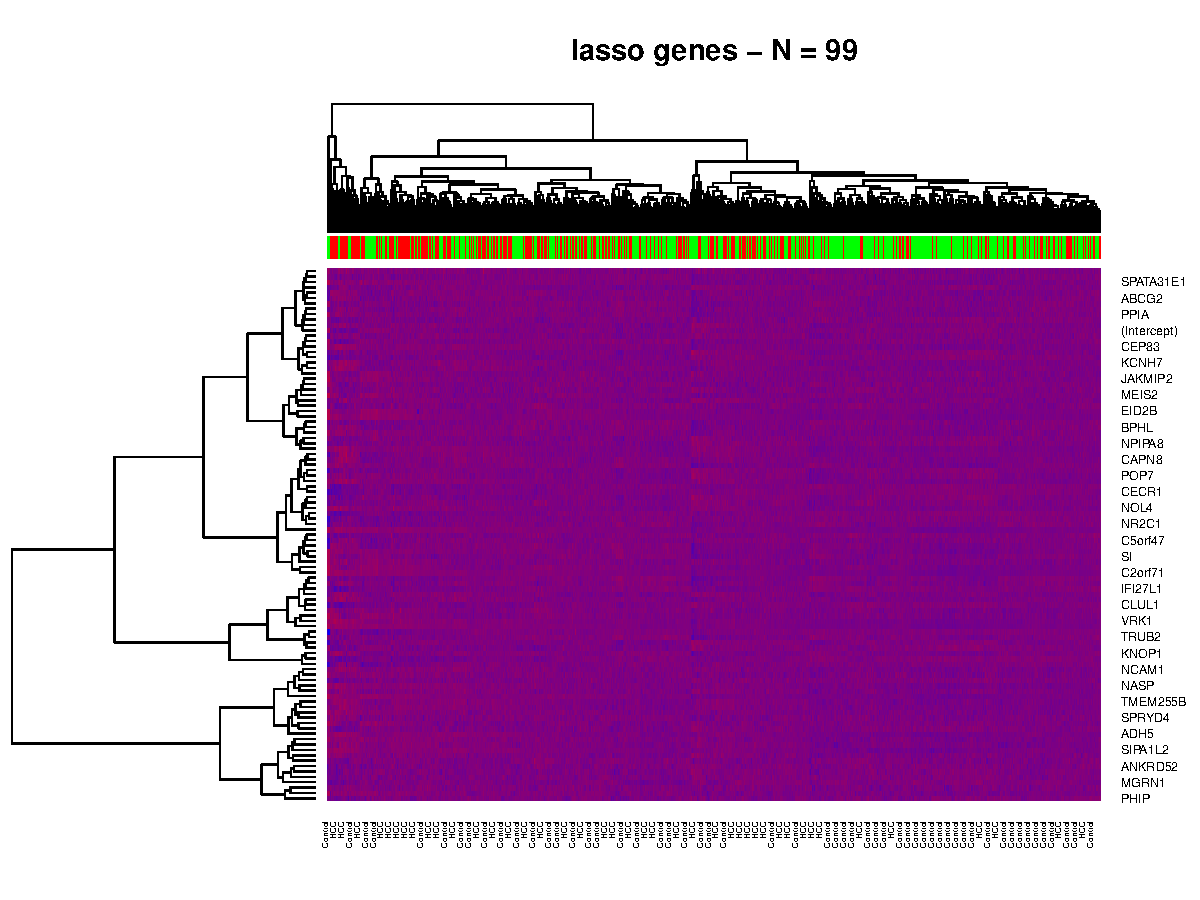
\includegraphics{Static/figures/heatmapLasso-1.pdf}
\caption{\label{fig:heatmapLasso}Lasso Model Genes}
\end{figure}

\begin{Shaded}
\begin{Highlighting}[]
 \KeywordTok{suppressPackageStartupMessages}\NormalTok{(}\KeywordTok{require}\NormalTok{(gplots))}

\CommentTok{\# train {-} cv predicted}
\NormalTok{enet\_coef <{-}}\StringTok{ }\KeywordTok{coef}\NormalTok{(}
\NormalTok{ cv\_enet,}
 \DataTypeTok{s=}\StringTok{\textquotesingle{}lambda.1se\textquotesingle{}}
\NormalTok{)}
\NormalTok{enet\_coef\_frm <{-}}\StringTok{ }\KeywordTok{data.frame}\NormalTok{(}
 \DataTypeTok{gene=}\NormalTok{enet\_coef}\OperatorTok{@}\NormalTok{Dimnames[[}\DecValTok{1}\NormalTok{]][}\KeywordTok{c}\NormalTok{(}\DecValTok{1}\NormalTok{, enet\_coef}\OperatorTok{@}\NormalTok{i[}\OperatorTok{{-}}\DecValTok{1}\NormalTok{])],}
 \DataTypeTok{enet=}\NormalTok{enet\_coef}\OperatorTok{@}\NormalTok{x)}

 
\NormalTok{  Mycol <{-}}\StringTok{ }\KeywordTok{colorpanel}\NormalTok{(}\DecValTok{1000}\NormalTok{, }\StringTok{"blue"}\NormalTok{, }\StringTok{"red"}\NormalTok{)}
  \KeywordTok{heatmap.2}\NormalTok{(}
    \DataTypeTok{x=}\KeywordTok{t}\NormalTok{(train\_lcpm\_mtx[,enet\_coef\_frm}\OperatorTok{$}\NormalTok{gene[}\OperatorTok{{-}}\DecValTok{1}\NormalTok{]]),}
    \DataTypeTok{scale=}\StringTok{"row"}\NormalTok{,}
    \DataTypeTok{labRow=}\NormalTok{enet\_coef\_frm}\OperatorTok{$}\NormalTok{gene,}
    \DataTypeTok{labCol=}\NormalTok{train\_group\_vec,}
    \DataTypeTok{col=}\NormalTok{Mycol, }
    \DataTypeTok{trace=}\StringTok{"none"}\NormalTok{, }\DataTypeTok{density.info=}\StringTok{"none"}\NormalTok{, }
    \CommentTok{\#margin=c(8,6), lhei=c(2,10), }
    \CommentTok{\#lwid=c(0.1,4), \#lhei=c(0.1,4)}
    \DataTypeTok{key=}\NormalTok{F,}
    \DataTypeTok{ColSideColors=}\KeywordTok{ifelse}\NormalTok{(train\_group\_vec}\OperatorTok{==}\StringTok{\textquotesingle{}Control\textquotesingle{}}\NormalTok{, }\StringTok{\textquotesingle{}green\textquotesingle{}}\NormalTok{,}\StringTok{\textquotesingle{}red\textquotesingle{}}\NormalTok{),}
    \DataTypeTok{dendrogram=}\StringTok{"both"}\NormalTok{,}
    \DataTypeTok{main=}\KeywordTok{paste}\NormalTok{(}\StringTok{\textquotesingle{}enet genes {-} N =\textquotesingle{}}\NormalTok{, }\KeywordTok{nrow}\NormalTok{(enet\_coef\_frm)}\OperatorTok{{-}}\DecValTok{1}\NormalTok{))}
\end{Highlighting}
\end{Shaded}

\begin{figure}
\centering
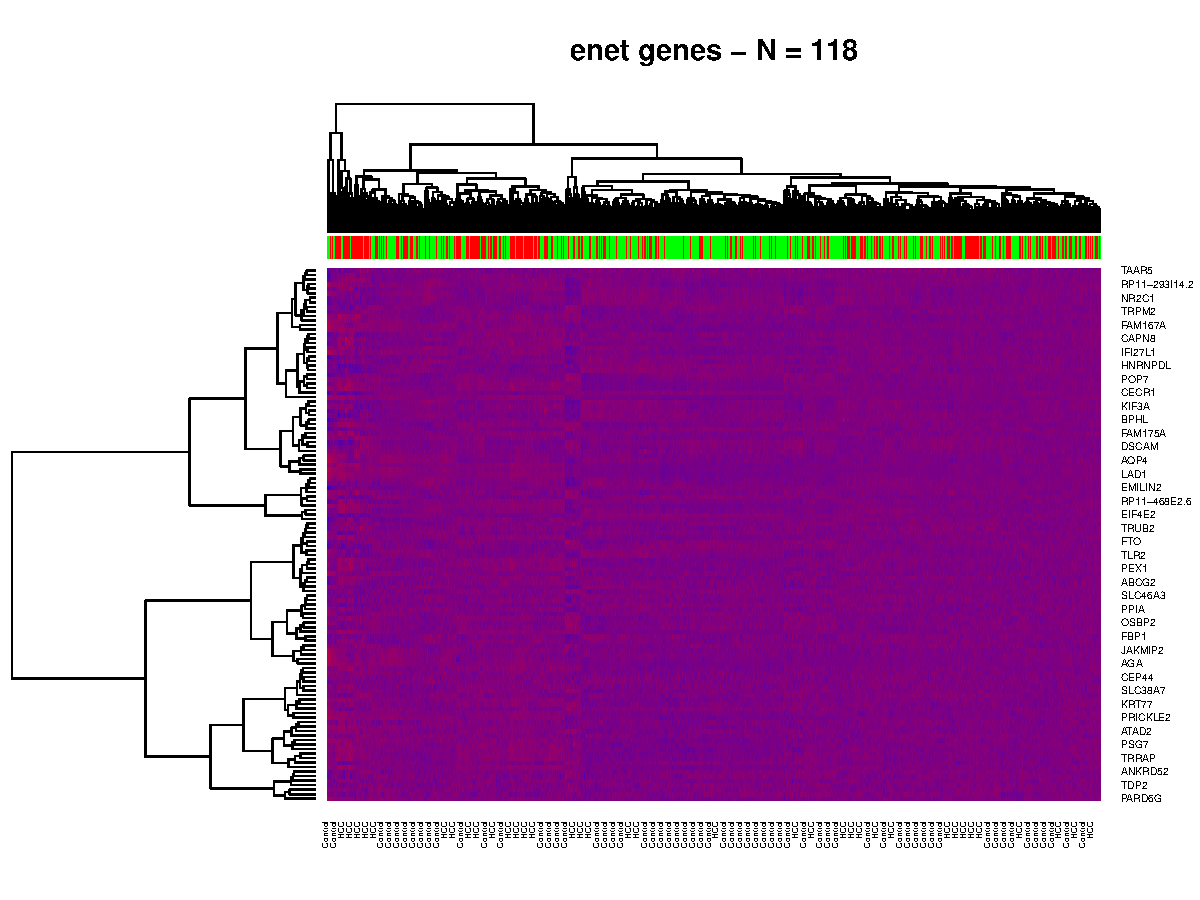
\includegraphics{Static/figures/heatmapEnet-1.pdf}
\caption{\label{fig:heatmapEnet}Enet Model Genes}
\end{figure}

\hypertarget{model-suite}{%
\chapter{Sample size investigation}\label{model-suite}}

We now examine the results of fitting a suite of lasso models to
investigate the effect of sample size on
various aspects of model performance:

\begin{itemize}
\item
  assessed accuracy: out-of-fold estimates of precision and variability vs train set estimates
\item
  selected feature profile stability - to what extent does the
  feature set implicitly selected by the lasso vary across random
  sampling and what is the effect of sample size.
\end{itemize}

It is hypothesized that below a certain threshold,
sample sizes are too small to provide reliable estimates
of performance or stable selected feature profiles.

In examining the relationship between sample size and
model performance, including variability and reliability
of performance indicators derived from fits, we should bear in
mind that in addition to sample size, sample composition might
also play a factor. If a training data set contains many outliers
or otherwise \emph{hard to properly classify} samples, the performance
of models fitted to such a data set is expected to be negatively impacted.

In the simulations that we run below we will track sample quality
to examine its impact on fitted model performance.
Predicted probabilities from fitted model can be transformed into sample
quality scores: \(Q_i = p_i^{y_i}(1-p_i)^{1-y_i}\), where \(p_i\) is the
estimated probability of HCC for sample i and \(y_i\) is 1 for HCC samples and
0 for Controls. ie. we use the fitted sample contribution to the
likelihood function as a sample quality score. To derive the sample quality scores,
we will use the predicted response from a lasso model fitted to the entire data set.

Hard to classify samples will have low quality scores.
In the results that we discuss below, when we look at variability across repeated
random sampling of different sizes, we can use sample quality scores to investigate
how much of the variability is due to sample selection.
Note that quality here is not used to say anything about the sample data quality.
Low quality here only means that a sample is different from the
core of the data set in a way that makes it hard to properly classify.
That could happen if the sample were mislabeled, in which case we could
think of this sample as being poor quality of course.

The variability in sample set \emph{quality} the we get from simple random sampling,
as is done in the simulation below, is not expected to adequately reflect
sample set quality variation encountered in practice when data for a particular
study are accumulated over extensive time horizons and across varied
physical settings. In order to accrue study samples at an acceptable rate,
it is not uncommon for the study sponsor to work with several clinics, medical centers,
or other tissue or blood sample provider. Or the sponsor may sub-contract the sample acquisition
task to a third party who may have suppliers distributed across the globe. This
is great news for the rate of sample acquisition, but not such great news for
the uniformity of quality of samples. In such a context, the variability
in sample set quality as the data set grows over time would not
be adequately captured by simple random sampling variability;
the variability would be more akin to cluster sampling with potential confounding
batch effects. The impact that these effects can have on the classification analysis
results cannot be understated, especially in the context of a new technology that
is exploiting biological processes that are still not fully understood. All this
to make the point that the variability the we are studying here has to be regarded
as a lower bound on the variability that is to be expected in practice, and that without
an external validation data set to verify results, one should be cautious
when interpreting empirical findings, especially in the absence of solid
biological underpinnings.

\hypertarget{full-data-set-fit}{%
\section{Full data set fit}\label{full-data-set-fit}}

We begin by fitting a model to the entire data set in order to:

\begin{itemize}
\item
  obtain a baseline clssification performance against which to judge the performance
  obtained from the fits to smaller sample sets,
\item
  obtain sample quality scores which can be used to explain variability
  in the performance of model fitted to data sets of a fixed size, and
\item
  produce a \emph{full model} gene signature which can be used to evaluate
  the stability of selected features in models fitted to data sets of diffferent
  sizes.
\end{itemize}

First assemble the data set. This entails simply re-combining the
train and test data.

\begin{Shaded}
\begin{Highlighting}[]
\CommentTok{\# combine train and test }
\NormalTok{all\_lcpm\_mtx <{-}}\StringTok{ }\KeywordTok{rbind}\NormalTok{(train\_lcpm\_mtx, test\_lcpm\_mtx)}

\CommentTok{\# we have to be careful with factors!}
\CommentTok{\# We\textquotesingle{}ll keep as a character and change to factor when needed}
\NormalTok{all\_group\_vec <{-}}\StringTok{ }\KeywordTok{c}\NormalTok{(}
 \KeywordTok{as.character}\NormalTok{(train\_group\_vec), }
 \KeywordTok{as.character}\NormalTok{(test\_group\_vec)}
\NormalTok{)}
\CommentTok{\# I suspect adding names to vectors breaks one of the tidy commandments,}
\CommentTok{\# but then again I am sure I have already offended the creed beyond salvation}
\KeywordTok{names}\NormalTok{(all\_group\_vec) <{-}}\StringTok{ }\KeywordTok{c}\NormalTok{(}
 \KeywordTok{names}\NormalTok{(train\_group\_vec),}
 \KeywordTok{names}\NormalTok{(test\_group\_vec)}
\NormalTok{)}

\NormalTok{knitr}\OperatorTok{::}\KeywordTok{kable}\NormalTok{(}\KeywordTok{table}\NormalTok{(}\DataTypeTok{group =}\NormalTok{ all\_group\_vec),}
  \DataTypeTok{caption =} \StringTok{"samples by group"}\NormalTok{) }\OperatorTok{\%>\%}
\StringTok{   }\NormalTok{kableExtra}\OperatorTok{::}\KeywordTok{kable\_styling}\NormalTok{(}\DataTypeTok{full\_width =}\NormalTok{ F)}
\end{Highlighting}
\end{Shaded}

\begin{table}

\caption{\label{tab:get-all-data}samples by group}
\centering
\begin{tabular}[t]{l|r}
\hline
group & Freq\\
\hline
Control & 778\\
\hline
HCC & 555\\
\hline
\end{tabular}
\end{table}

Now fit the losso model through cross-validation.
Note that the results of a cv fit are random due to the
random allocation of samples to folds. We can reduce this
varibility by properly averaging results over repeated cv fits.
Here we will obtain sample quality scores by averaging results
over 30 cv runs.

\begin{Shaded}
\begin{Highlighting}[]
\KeywordTok{set.seed}\NormalTok{(}\DecValTok{1}\NormalTok{)}

\NormalTok{start\_time <{-}}\StringTok{  }\KeywordTok{proc.time}\NormalTok{()}

\NormalTok{cv\_lassoAll\_lst <{-}}\StringTok{ }\KeywordTok{lapply}\NormalTok{(}\DecValTok{1}\OperatorTok{:}\DecValTok{30}\NormalTok{, }\ControlFlowTok{function}\NormalTok{(REP) \{}
\NormalTok{glmnet}\OperatorTok{::}\KeywordTok{cv.glmnet}\NormalTok{(}
 \DataTypeTok{x =}\NormalTok{ all\_lcpm\_mtx,}
 \DataTypeTok{y =} \KeywordTok{factor}\NormalTok{(all\_group\_vec,}\DataTypeTok{levels =} \KeywordTok{c}\NormalTok{(}\StringTok{\textquotesingle{}Control\textquotesingle{}}\NormalTok{, }\StringTok{\textquotesingle{}HCC\textquotesingle{}}\NormalTok{)),}
 \DataTypeTok{alpha =} \DecValTok{1}\NormalTok{,}
 \DataTypeTok{family =} \StringTok{\textquotesingle{}binomial\textquotesingle{}}\NormalTok{,}
 \DataTypeTok{type.measure  =}  \StringTok{"class"}\NormalTok{,}
 \DataTypeTok{keep =}\NormalTok{ T,}
 \DataTypeTok{nlambda =} \DecValTok{100}
\NormalTok{)}
\NormalTok{\}}
\NormalTok{)}

\KeywordTok{message}\NormalTok{(}\StringTok{"lassoAll time: "}\NormalTok{, }\KeywordTok{round}\NormalTok{((}\KeywordTok{proc.time}\NormalTok{() }\OperatorTok{{-}}\StringTok{ }\NormalTok{start\_time)[}\DecValTok{3}\NormalTok{],}\DecValTok{2}\NormalTok{),}\StringTok{"s"}\NormalTok{)}
\end{Highlighting}
\end{Shaded}

Examine the fits.

\begin{Shaded}
\begin{Highlighting}[]
\CommentTok{\#\#\# CLEAR CACHE}
\KeywordTok{plot}\NormalTok{(}
 \KeywordTok{log}\NormalTok{(cv\_lassoAll\_lst[[}\DecValTok{1}\NormalTok{]]}\OperatorTok{$}\NormalTok{lambda),}
\NormalTok{ cv\_lassoAll\_lst[[}\DecValTok{1}\NormalTok{]]}\OperatorTok{$}\NormalTok{cvm,}
 \DataTypeTok{lwd=}\DecValTok{2}\NormalTok{,}
 \DataTypeTok{xlab=}\StringTok{\textquotesingle{}log(Lambda)\textquotesingle{}}\NormalTok{, }\DataTypeTok{ylab=}\StringTok{\textquotesingle{}CV Misclassification Error\textquotesingle{}}\NormalTok{, }\DataTypeTok{type=}\StringTok{\textquotesingle{}l\textquotesingle{}}\NormalTok{, }\DataTypeTok{ylim=}\KeywordTok{c}\NormalTok{(}\DecValTok{0}\NormalTok{, }\FloatTok{.5}\NormalTok{)}
\NormalTok{)}

\ControlFlowTok{for}\NormalTok{(JJ }\ControlFlowTok{in} \DecValTok{2}\OperatorTok{:}\KeywordTok{length}\NormalTok{(cv\_lassoAll\_lst))}
 \KeywordTok{lines}\NormalTok{(}
  \KeywordTok{log}\NormalTok{(cv\_lassoAll\_lst[[JJ]]}\OperatorTok{$}\NormalTok{lambda),}
\NormalTok{  cv\_lassoAll\_lst[[JJ]]}\OperatorTok{$}\NormalTok{cvm,}
  \DataTypeTok{lwd=}\DecValTok{2}
\NormalTok{)}
\end{Highlighting}
\end{Shaded}

\begin{figure}
\centering
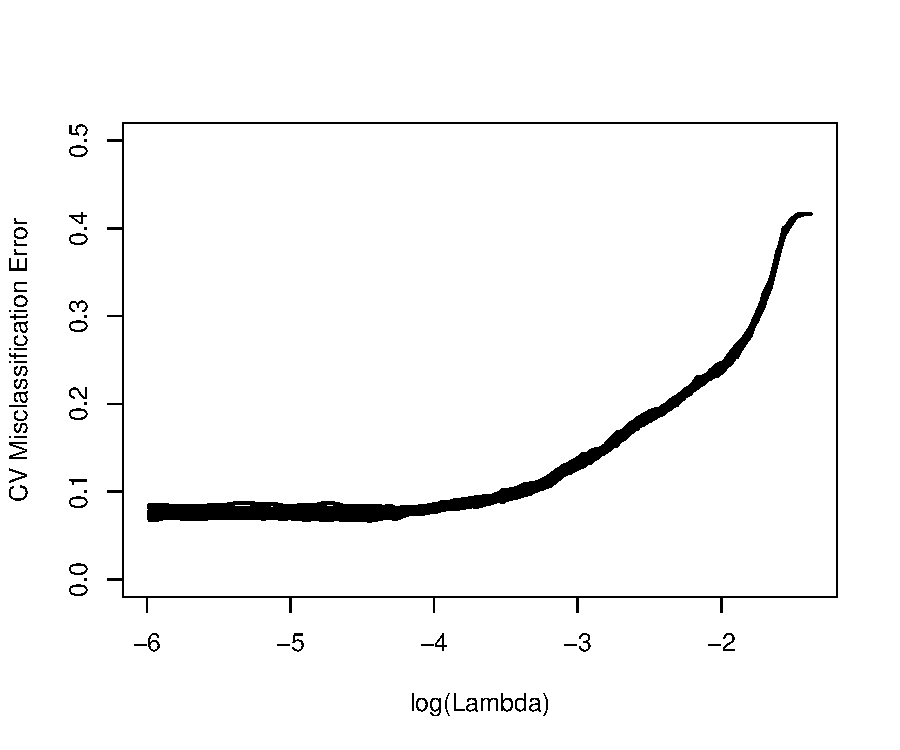
\includegraphics{Static/figures/plot-lassoAll-1.pdf}
\caption{\label{fig:plot-lassoAll}Repeated cv lasso models fitted to all samples}
\end{figure}

These cv curves are remarkably consistent meaning that the determination of the size or sparsity
of the model fitted through cross validation to the full data set is fairly precise:

\begin{Shaded}
\begin{Highlighting}[]
\KeywordTok{library}\NormalTok{(magrittr)}

\KeywordTok{par}\NormalTok{(}\DataTypeTok{mfrow=}\KeywordTok{c}\NormalTok{(}\DecValTok{1}\NormalTok{,}\DecValTok{2}\NormalTok{), }\DataTypeTok{mar=}\KeywordTok{c}\NormalTok{(}\DecValTok{3}\NormalTok{,}\DecValTok{4}\NormalTok{, }\DecValTok{2}\NormalTok{, }\DecValTok{1}\NormalTok{))}

\CommentTok{\# nzero}
\NormalTok{nzero\_1se\_vec <{-}}\StringTok{ }\KeywordTok{sapply}\NormalTok{(cv\_lassoAll\_lst,}
 \ControlFlowTok{function}\NormalTok{(cv\_fit) cv\_fit}\OperatorTok{$}\NormalTok{nzero[cv\_fit}\OperatorTok{$}\NormalTok{lambda }\OperatorTok{==}\StringTok{ }\NormalTok{cv\_fit}\OperatorTok{$}\NormalTok{lambda}\FloatTok{.1}\NormalTok{se])}

\NormalTok{nzero\_min\_vec <{-}}\StringTok{ }\KeywordTok{sapply}\NormalTok{(cv\_lassoAll\_lst,}
 \ControlFlowTok{function}\NormalTok{(cv\_fit) cv\_fit}\OperatorTok{$}\NormalTok{nzero[cv\_fit}\OperatorTok{$}\NormalTok{lambda }\OperatorTok{==}\StringTok{ }\NormalTok{cv\_fit}\OperatorTok{$}\NormalTok{lambda.min])}

\KeywordTok{boxplot}\NormalTok{(}\KeywordTok{list}\NormalTok{(}\StringTok{\textasciigrave{}}\DataTypeTok{1se}\StringTok{\textasciigrave{}}\NormalTok{=nzero\_1se\_vec, }\DataTypeTok{min =}\NormalTok{ nzero\_min\_vec), }\DataTypeTok{ylab=}\StringTok{"Selected Features"}\NormalTok{)}

\CommentTok{\# error}
\NormalTok{error\_1se\_vec <{-}}\StringTok{ }\KeywordTok{sapply}\NormalTok{(cv\_lassoAll\_lst,}
 \ControlFlowTok{function}\NormalTok{(cv\_fit) cv\_fit}\OperatorTok{$}\NormalTok{cvm[cv\_fit}\OperatorTok{$}\NormalTok{lambda }\OperatorTok{==}\StringTok{ }\NormalTok{cv\_fit}\OperatorTok{$}\NormalTok{lambda}\FloatTok{.1}\NormalTok{se])}

\NormalTok{error\_min\_vec <{-}}\StringTok{ }\KeywordTok{sapply}\NormalTok{(cv\_lassoAll\_lst,}
 \ControlFlowTok{function}\NormalTok{(cv\_fit) cv\_fit}\OperatorTok{$}\NormalTok{cvm[cv\_fit}\OperatorTok{$}\NormalTok{lambda }\OperatorTok{==}\StringTok{ }\NormalTok{cv\_fit}\OperatorTok{$}\NormalTok{lambda.min])}

\KeywordTok{boxplot}\NormalTok{(}
 \KeywordTok{list}\NormalTok{(}\StringTok{\textasciigrave{}}\DataTypeTok{1se}\StringTok{\textasciigrave{}}\NormalTok{=error\_1se\_vec, }\DataTypeTok{min =}\NormalTok{ error\_min\_vec), }
 \DataTypeTok{ylab=}\NormalTok{cv\_lassoAll\_lst[[}\DecValTok{1}\NormalTok{]]}\OperatorTok{$}\NormalTok{name,}
 \DataTypeTok{ylim=}\KeywordTok{c}\NormalTok{(}\FloatTok{0.06}\NormalTok{, }\FloatTok{.10}\NormalTok{)}
\NormalTok{)}
\end{Highlighting}
\end{Shaded}

\begin{figure}
\centering
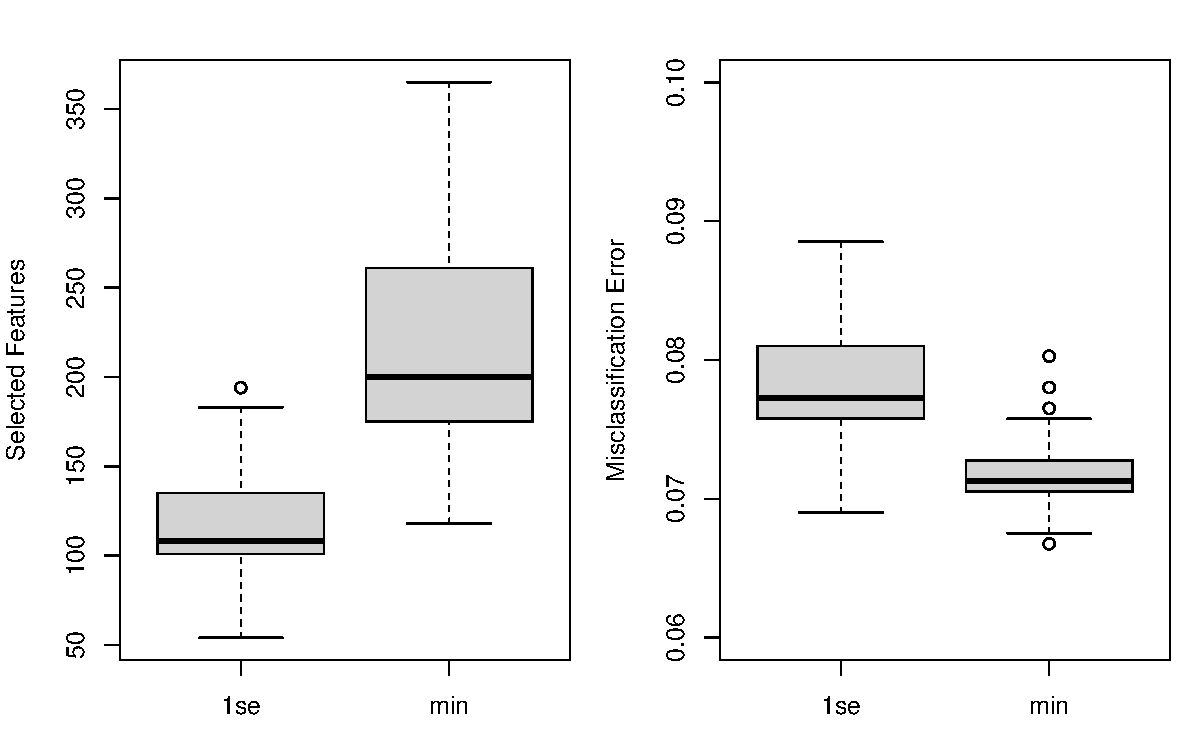
\includegraphics{Static/figures/model-size-lassoAll-1.pdf}
\caption{\label{fig:model-size-lassoAll}Feature selection and estimated error by repeated cv lasso models}
\end{figure}

\begin{Shaded}
\begin{Highlighting}[]
\CommentTok{\# tabular format}
\NormalTok{tmp <{-}}\StringTok{ }\KeywordTok{data.frame}\NormalTok{(}\KeywordTok{rbind}\NormalTok{(}
 \StringTok{\textasciigrave{}}\DataTypeTok{features\_1se}\StringTok{\textasciigrave{}}\NormalTok{ =}\StringTok{ }\KeywordTok{summary}\NormalTok{(nzero\_1se\_vec),}
 \DataTypeTok{features\_min =} \KeywordTok{summary}\NormalTok{(nzero\_min\_vec),}
 \StringTok{\textasciigrave{}}\DataTypeTok{features:min{-}1se}\StringTok{\textasciigrave{}}\NormalTok{ =}\StringTok{ }\KeywordTok{summary}\NormalTok{(nzero\_min\_vec }\OperatorTok{{-}}\StringTok{ }\NormalTok{nzero\_1se\_vec),}
 \StringTok{\textasciigrave{}}\DataTypeTok{cv\_error\_1se}\StringTok{\textasciigrave{}}\NormalTok{ =}\StringTok{ }\KeywordTok{summary}\NormalTok{(}\DecValTok{100}\OperatorTok{*}\NormalTok{error\_1se\_vec),}
 \DataTypeTok{cv\_error\_min =} \KeywordTok{summary}\NormalTok{(}\DecValTok{100}\OperatorTok{*}\NormalTok{error\_min\_vec),}
 \StringTok{\textasciigrave{}}\DataTypeTok{cv\_error:1se{-}min}\StringTok{\textasciigrave{}}\NormalTok{ =}\StringTok{ }\KeywordTok{summary}\NormalTok{(}\DecValTok{100}\OperatorTok{*}\NormalTok{(error\_1se\_vec}\OperatorTok{{-}}\NormalTok{error\_min\_vec))}
\NormalTok{))}

\NormalTok{knitr}\OperatorTok{::}\KeywordTok{kable}\NormalTok{(tmp }\OperatorTok{\%>\%}\StringTok{ }\NormalTok{dplyr}\OperatorTok{::}\KeywordTok{select}\NormalTok{(}\OperatorTok{{-}}\NormalTok{Mean),}
  \DataTypeTok{caption =} \StringTok{"Number of selected features"}\NormalTok{,}
  \DataTypeTok{digits=}\DecValTok{1}\NormalTok{) }\OperatorTok{\%>\%}
\StringTok{   }\NormalTok{kableExtra}\OperatorTok{::}\KeywordTok{kable\_styling}\NormalTok{(}\DataTypeTok{full\_width =}\NormalTok{ F)}
\end{Highlighting}
\end{Shaded}

\begin{table}

\caption{\label{tab:model-size-lassoAll}Number of selected features}
\centering
\begin{tabular}[t]{l|r|r|r|r|r}
\hline
  & Min. & X1st.Qu. & Median & X3rd.Qu. & Max.\\
\hline
features\_1se & 54.0 & 102.0 & 108.0 & 132.5 & 194.0\\
\hline
features\_min & 118.0 & 175.2 & 200.0 & 261.0 & 365.0\\
\hline
features:min-1se & 10.0 & 55.0 & 86.0 & 141.5 & 247.0\\
\hline
cv\_error\_1se & 6.9 & 7.6 & 7.7 & 8.1 & 8.9\\
\hline
cv\_error\_min & 6.7 & 7.1 & 7.1 & 7.3 & 8.0\\
\hline
cv\_error:1se-min & 0.2 & 0.5 & 0.6 & 0.7 & 1.0\\
\hline
\end{tabular}
\end{table}

The number of features selected by the minimum lambda models are larger
than the number selected by the ``one standard error'' rule models by a median
of \(86\).
The cv error rates obtained from the minimum lambda models are lower
then ``one standard error'' rule models error rates by a median of
\(0.6\)\%.

The cv error rates observed in this set are comparable to the
rates oberved in the lasso models fitted to the training sample set
which consisted of 80\% of the samples in this set. In other words,
there is no obvious gain in performance in moving from
a data set with
\(622 vs 444\) samples
to a data set with
\(778 vs 555\) samples.
See Table \ref{tab:printErrors}.

It's not clear at this point whether the minimum lambda model is truly better than
the ``one standard error'' rule model. We would need and external validation
set to make this determination. We can compare the two sets
of out-of-fold predicted values, averaged across cv replicates, to see if
there is a meaningful difference between the two.

\begin{Shaded}
\begin{Highlighting}[]
\CommentTok{\# predicted probs {-} 1se}
\NormalTok{lassoAll\_predResp\_1se\_mtx <{-}}\StringTok{ }\KeywordTok{sapply}\NormalTok{(cv\_lassoAll\_lst, }\ControlFlowTok{function}\NormalTok{(cv\_fit) \{ }
\NormalTok{  ndx\_1se <{-}}\StringTok{ }\KeywordTok{match}\NormalTok{(cv\_fit}\OperatorTok{$}\NormalTok{lambda}\FloatTok{.1}\NormalTok{se,cv\_fit}\OperatorTok{$}\NormalTok{lambda)}
  \KeywordTok{logistic\_f}\NormalTok{(cv\_fit}\OperatorTok{$}\NormalTok{fit.preval[,ndx\_1se])}
\NormalTok{ \})}
\NormalTok{lassoAll\_predResp\_1se\_vec <{-}}\StringTok{ }\KeywordTok{rowMeans}\NormalTok{(lassoAll\_predResp\_1se\_mtx)}

\CommentTok{\# predicted probs {-} min}
\NormalTok{lassoAll\_predResp\_min\_mtx <{-}}\StringTok{ }\KeywordTok{sapply}\NormalTok{(cv\_lassoAll\_lst, }\ControlFlowTok{function}\NormalTok{(cv\_fit) \{ }
\NormalTok{  ndx\_min <{-}}\StringTok{ }\KeywordTok{match}\NormalTok{(cv\_fit}\OperatorTok{$}\NormalTok{lambda.min,cv\_fit}\OperatorTok{$}\NormalTok{lambda)}
  \KeywordTok{logistic\_f}\NormalTok{(cv\_fit}\OperatorTok{$}\NormalTok{fit.preval[,ndx\_min])}
\NormalTok{ \})}
\NormalTok{lassoAll\_predResp\_min\_vec <{-}}\StringTok{ }\KeywordTok{rowMeans}\NormalTok{(lassoAll\_predResp\_min\_mtx)}

\CommentTok{\# plot}
\KeywordTok{par}\NormalTok{(}\DataTypeTok{mfrow=}\KeywordTok{c}\NormalTok{(}\DecValTok{1}\NormalTok{,}\DecValTok{2}\NormalTok{), }\DataTypeTok{mar=}\KeywordTok{c}\NormalTok{(}\DecValTok{5}\NormalTok{,}\DecValTok{5}\NormalTok{,}\DecValTok{2}\NormalTok{,}\DecValTok{1}\NormalTok{))}
\NormalTok{tmp <{-}}\StringTok{ }\KeywordTok{c}\NormalTok{(}
 \StringTok{\textasciigrave{}}\DataTypeTok{1se}\StringTok{\textasciigrave{}}\NormalTok{ =}\StringTok{ }\KeywordTok{split}\NormalTok{(lassoAll\_predResp\_1se\_vec, all\_group\_vec),}
 \DataTypeTok{min =} \KeywordTok{split}\NormalTok{(lassoAll\_predResp\_min\_vec, all\_group\_vec)}
\NormalTok{)}
\KeywordTok{names}\NormalTok{(tmp) <{-}}\StringTok{ }\KeywordTok{sub}\NormalTok{(}\StringTok{\textquotesingle{}}\CharTok{\textbackslash{}\textbackslash{}}\StringTok{.\textquotesingle{}}\NormalTok{, }\StringTok{\textquotesingle{}}\CharTok{\textbackslash{}n}\StringTok{\textquotesingle{}}\NormalTok{, }\KeywordTok{names}\NormalTok{(tmp))}

\KeywordTok{boxplot}\NormalTok{(}
\NormalTok{ tmp,}
 \DataTypeTok{ylab=}\StringTok{\textquotesingle{}Predicted oof probability\textquotesingle{}}\NormalTok{,}
 \DataTypeTok{border=}\KeywordTok{c}\NormalTok{(}\StringTok{\textquotesingle{}green\textquotesingle{}}\NormalTok{, }\StringTok{\textquotesingle{}red\textquotesingle{}}\NormalTok{),}
 \DataTypeTok{xaxt=}\StringTok{\textquotesingle{}n\textquotesingle{}}
\NormalTok{)}
\KeywordTok{axis}\NormalTok{(}\DataTypeTok{side=}\DecValTok{1}\NormalTok{, }\DataTypeTok{at=}\DecValTok{1}\OperatorTok{:}\KeywordTok{length}\NormalTok{(tmp), }\DataTypeTok{tick=}\NormalTok{F, }\KeywordTok{names}\NormalTok{(tmp))}


\CommentTok{\# compare the two}
\KeywordTok{plot}\NormalTok{(}
 \DataTypeTok{x =}\NormalTok{ lassoAll\_predResp\_1se\_vec, }\DataTypeTok{xlab=}\StringTok{\textquotesingle{}1se model oof Prob\textquotesingle{}}\NormalTok{,}
 \DataTypeTok{y =}\NormalTok{ lassoAll\_predResp\_min\_vec, }\DataTypeTok{ylab=}\StringTok{\textquotesingle{}min lambda model oof Prob\textquotesingle{}}\NormalTok{,}
 \DataTypeTok{col =} \KeywordTok{ifelse}\NormalTok{(all\_group\_vec }\OperatorTok{==}\StringTok{ \textquotesingle{}HCC\textquotesingle{}}\NormalTok{, }\StringTok{\textquotesingle{}red\textquotesingle{}}\NormalTok{, }\StringTok{\textquotesingle{}green\textquotesingle{}}\NormalTok{)}
\NormalTok{)}
 
\CommentTok{\# Add referecne lines at 10\% false positive}
\NormalTok{thres\_1se <{-}}\StringTok{ }\KeywordTok{quantile}\NormalTok{(lassoAll\_predResp\_1se\_vec[all\_group\_vec }\OperatorTok{==}\StringTok{ \textquotesingle{}Control\textquotesingle{}}\NormalTok{], }\DataTypeTok{prob=}\NormalTok{.}\DecValTok{9}\NormalTok{)}
\NormalTok{thres\_min <{-}}\StringTok{ }\KeywordTok{quantile}\NormalTok{(lassoAll\_predResp\_min\_vec[all\_group\_vec }\OperatorTok{==}\StringTok{ \textquotesingle{}Control\textquotesingle{}}\NormalTok{], }\DataTypeTok{prob=}\NormalTok{.}\DecValTok{9}\NormalTok{)}
\KeywordTok{abline}\NormalTok{(}\DataTypeTok{v =}\NormalTok{ thres\_1se, }\DataTypeTok{h =}\NormalTok{ thres\_min, }\DataTypeTok{col=}\StringTok{\textquotesingle{}grey\textquotesingle{}}\NormalTok{)}
\end{Highlighting}
\end{Shaded}

\begin{figure}
\centering
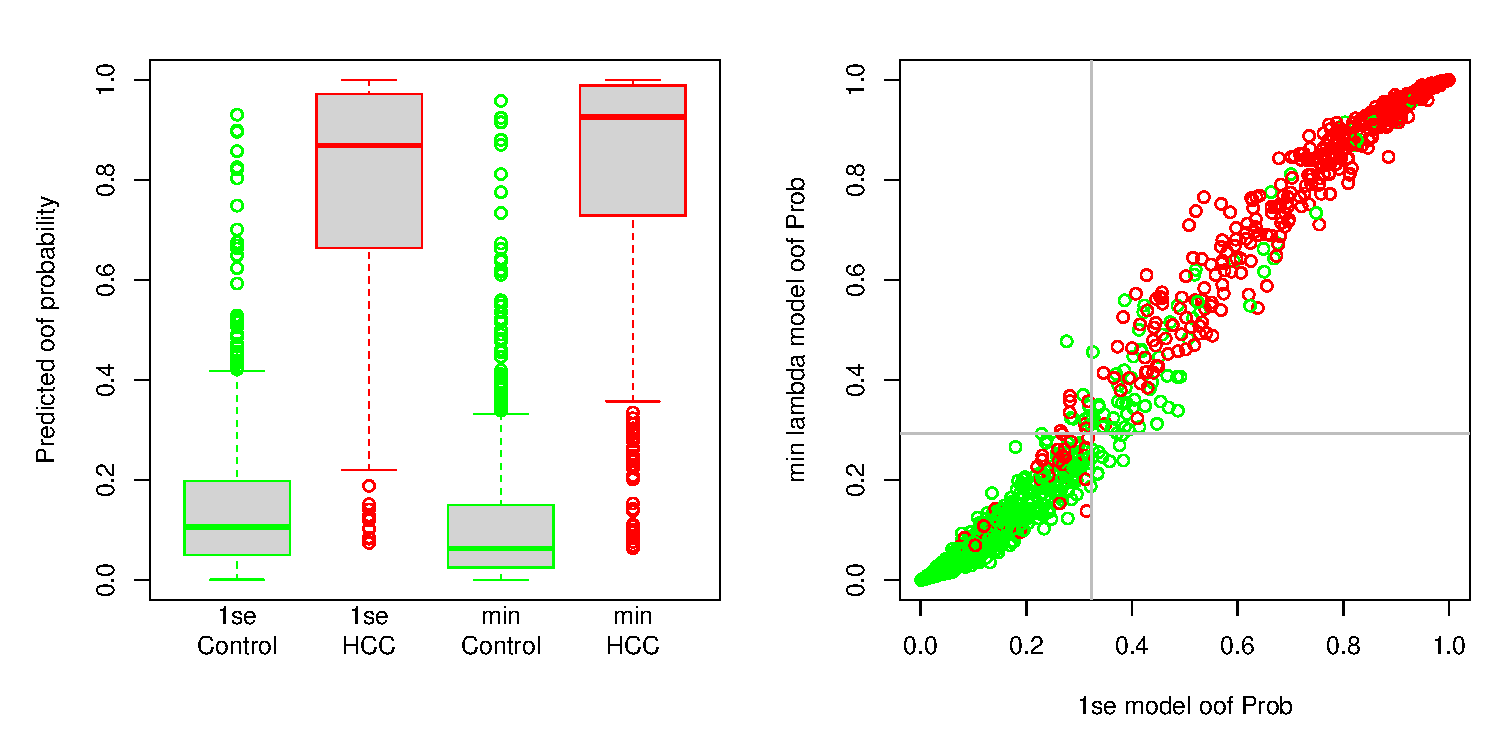
\includegraphics{Static/figures/get-sample-pred-1.pdf}
\caption{\label{fig:get-sample-pred}Predicted probabilities - averaged over cv replicates}
\end{figure}

We see that there isn't a big difference in out-of-fold predicted
probabilities between the one-standard-error rule and the minimum lamda models.
One way to quantify
the difference in classification errors is to classify samples
according to each vector of predicted probabilities, setting
the thresholds to achieve a fixed false positive rate, 10\% say.
These thresholds are indicated by the grey lines in the scatter plot
on the right side of Figure \ref{fig:get-sample-pred}.

\begin{Shaded}
\begin{Highlighting}[]
\NormalTok{lassoAll\_predClass\_1se\_vec <{-}}\StringTok{ }\KeywordTok{ifelse}\NormalTok{(}
\NormalTok{ lassoAll\_predResp\_1se\_vec }\OperatorTok{>}\StringTok{ }\NormalTok{thres\_1se, }\StringTok{\textquotesingle{}HCC\textquotesingle{}}\NormalTok{, }\StringTok{\textquotesingle{}Control\textquotesingle{}}\NormalTok{)}

\NormalTok{lassoAll\_predClass\_min\_vec <{-}}\StringTok{ }\KeywordTok{ifelse}\NormalTok{(}
\NormalTok{ lassoAll\_predResp\_min\_vec }\OperatorTok{>}\StringTok{ }\NormalTok{thres\_min, }\StringTok{\textquotesingle{}HCC\textquotesingle{}}\NormalTok{, }\StringTok{\textquotesingle{}Control\textquotesingle{}}\NormalTok{)}

\NormalTok{tmp <{-}}\StringTok{ }\KeywordTok{cbind}\NormalTok{(}
 \KeywordTok{table}\NormalTok{(}\DataTypeTok{truth=}\NormalTok{all\_group\_vec, }\StringTok{\textasciigrave{}}\DataTypeTok{1se{-}pred}\StringTok{\textasciigrave{}}\NormalTok{=lassoAll\_predClass\_1se\_vec),}
 \KeywordTok{table}\NormalTok{(}\DataTypeTok{truth=}\NormalTok{all\_group\_vec, }\StringTok{\textasciigrave{}}\DataTypeTok{min{-}pred}\StringTok{\textasciigrave{}}\NormalTok{=lassoAll\_predClass\_min\_vec)}
\NormalTok{) }
\CommentTok{\# Hack for printing}
\KeywordTok{colnames}\NormalTok{(tmp) <{-}}\StringTok{ }\KeywordTok{c}\NormalTok{(}\StringTok{\textquotesingle{}1se{-}Control\textquotesingle{}}\NormalTok{, }\StringTok{\textquotesingle{}1se{-}HCC\textquotesingle{}}\NormalTok{, }\StringTok{\textquotesingle{}min{-}Control\textquotesingle{}}\NormalTok{, }\StringTok{\textquotesingle{}min{-}HCC\textquotesingle{}}\NormalTok{)}

\NormalTok{knitr}\OperatorTok{::}\KeywordTok{kable}\NormalTok{(tmp,}
  \DataTypeTok{caption =} \StringTok{"Classifications: rows are truth"}\NormalTok{,}
  \DataTypeTok{digits=}\DecValTok{1}\NormalTok{) }\OperatorTok{\%>\%}
\StringTok{   }\NormalTok{kableExtra}\OperatorTok{::}\KeywordTok{kable\_styling}\NormalTok{(}\DataTypeTok{full\_width =}\NormalTok{ F)}
\end{Highlighting}
\end{Shaded}

\begin{table}

\caption{\label{tab:get-sample-class}Classifications: rows are truth}
\centering
\begin{tabular}[t]{l|r|r|r|r}
\hline
  & 1se-Control & 1se-HCC & min-Control & min-HCC\\
\hline
Control & 700 & 78 & 700 & 78\\
\hline
HCC & 39 & 516 & 32 & 523\\
\hline
\end{tabular}
\end{table}

When we fix the false positive rate at 10\% (ie. the control samples error rates are fixed),
the \texttt{1se} model makes 39 false negative calls whereas the minimum lambda model makes 32. A difference
of \(1.3\)\%

\hypertarget{get-sample-quality-scores}{%
\subsection*{Get sample quality scores}\label{get-sample-quality-scores}}
\addcontentsline{toc}{subsection}{Get sample quality scores}

To compute quality scores, we will use the out-of-fold predicted probabilities.

\begin{Shaded}
\begin{Highlighting}[]
\CommentTok{\# get qual scores}

\NormalTok{y <{-}}\StringTok{ }\KeywordTok{as.numeric}\NormalTok{(all\_group\_vec }\OperatorTok{==}\StringTok{ \textquotesingle{}HCC\textquotesingle{}}\NormalTok{)}
\CommentTok{\# 1se}
\NormalTok{p <{-}}\StringTok{ }\NormalTok{lassoAll\_predResp\_1se\_vec}
\NormalTok{sample\_1se\_qual\_vec <{-}}\StringTok{ }\NormalTok{p}\OperatorTok{\^{}}\NormalTok{y}\OperatorTok{*}\NormalTok{(}\DecValTok{1}\OperatorTok{{-}}\NormalTok{p)}\OperatorTok{\^{}}\NormalTok{(}\DecValTok{1}\OperatorTok{{-}}\NormalTok{y)}

\CommentTok{\# min}
\NormalTok{p <{-}}\StringTok{ }\NormalTok{lassoAll\_predResp\_min\_vec}
\NormalTok{sample\_min\_qual\_vec <{-}}\StringTok{ }\NormalTok{p}\OperatorTok{\^{}}\NormalTok{y}\OperatorTok{*}\NormalTok{(}\DecValTok{1}\OperatorTok{{-}}\NormalTok{p)}\OperatorTok{\^{}}\NormalTok{(}\DecValTok{1}\OperatorTok{{-}}\NormalTok{y)}
\end{Highlighting}
\end{Shaded}

We can examine quality scores as a function of classification bin.

\begin{Shaded}
\begin{Highlighting}[]
\NormalTok{y <{-}}\StringTok{ }\KeywordTok{as.numeric}\NormalTok{(all\_group\_vec }\OperatorTok{==}\StringTok{ \textquotesingle{}HCC\textquotesingle{}}\NormalTok{)}

\CommentTok{\# 1se}
\NormalTok{lassoAll\_1se\_conf\_vec <{-}}\StringTok{ }\KeywordTok{paste}\NormalTok{(}
\NormalTok{ y, }
 \KeywordTok{as.numeric}\NormalTok{(lassoAll\_predClass\_1se\_vec}\OperatorTok{==}\StringTok{\textquotesingle{}HCC\textquotesingle{}}\NormalTok{),}
 \DataTypeTok{sep =} \StringTok{\textquotesingle{}:\textquotesingle{}}
\NormalTok{)}

\CommentTok{\# min}
\NormalTok{lassoAll\_min\_conf\_vec <{-}}\StringTok{ }\KeywordTok{paste}\NormalTok{(}
\NormalTok{ y, }
 \KeywordTok{as.numeric}\NormalTok{(lassoAll\_predClass\_min\_vec}\OperatorTok{==}\StringTok{\textquotesingle{}HCC\textquotesingle{}}\NormalTok{),}
 \DataTypeTok{sep =} \StringTok{\textquotesingle{}:\textquotesingle{}}
\NormalTok{)}


\NormalTok{tmp <{-}}\StringTok{ }\KeywordTok{c}\NormalTok{(}
 \KeywordTok{split}\NormalTok{(sample\_1se\_qual\_vec, lassoAll\_1se\_conf\_vec), }
 \KeywordTok{split}\NormalTok{(sample\_min\_qual\_vec, lassoAll\_min\_conf\_vec)}
\NormalTok{)}

\KeywordTok{par}\NormalTok{(}\DataTypeTok{mfrow=}\KeywordTok{c}\NormalTok{(}\DecValTok{1}\NormalTok{,}\DecValTok{2}\NormalTok{), }\DataTypeTok{mar=}\KeywordTok{c}\NormalTok{(}\DecValTok{4}\NormalTok{,}\DecValTok{3}\NormalTok{,}\DecValTok{3}\NormalTok{,}\DecValTok{2}\NormalTok{), }\DataTypeTok{oma=}\KeywordTok{c}\NormalTok{(}\DecValTok{2}\NormalTok{,}\DecValTok{2}\NormalTok{,}\DecValTok{2}\NormalTok{,}\DecValTok{0}\NormalTok{))}
\NormalTok{gplots}\OperatorTok{::}\KeywordTok{boxplot2}\NormalTok{(}\KeywordTok{split}\NormalTok{(sample\_1se\_qual\_vec, lassoAll\_1se\_conf\_vec), }
  \DataTypeTok{outline=}\NormalTok{F, }\DataTypeTok{ylab =} \StringTok{\textquotesingle{}\textquotesingle{}}\NormalTok{, }
  \DataTypeTok{border=}\KeywordTok{c}\NormalTok{(}\StringTok{\textquotesingle{}green\textquotesingle{}}\NormalTok{, }\StringTok{\textquotesingle{}green\textquotesingle{}}\NormalTok{, }\StringTok{\textquotesingle{}red\textquotesingle{}}\NormalTok{, }\StringTok{\textquotesingle{}red\textquotesingle{}}\NormalTok{),}
  \DataTypeTok{ylim=}\KeywordTok{c}\NormalTok{(}\DecValTok{0}\NormalTok{,}\DecValTok{1}\NormalTok{))}
\KeywordTok{title}\NormalTok{(}\StringTok{\textquotesingle{}1se Model\textquotesingle{}}\NormalTok{)}

\NormalTok{gplots}\OperatorTok{::}\KeywordTok{boxplot2}\NormalTok{(}\KeywordTok{split}\NormalTok{(sample\_min\_qual\_vec, lassoAll\_min\_conf\_vec), }
  \DataTypeTok{outline=}\NormalTok{F, }\DataTypeTok{ylab =} \StringTok{\textquotesingle{}\textquotesingle{}}\NormalTok{,}
  \DataTypeTok{border=}\KeywordTok{c}\NormalTok{(}\StringTok{\textquotesingle{}green\textquotesingle{}}\NormalTok{, }\StringTok{\textquotesingle{}green\textquotesingle{}}\NormalTok{, }\StringTok{\textquotesingle{}red\textquotesingle{}}\NormalTok{, }\StringTok{\textquotesingle{}red\textquotesingle{}}\NormalTok{),}
  \DataTypeTok{ylim=}\KeywordTok{c}\NormalTok{(}\DecValTok{0}\NormalTok{,}\DecValTok{1}\NormalTok{))}
\KeywordTok{title}\NormalTok{(}\StringTok{\textquotesingle{}min lambda Model\textquotesingle{}}\NormalTok{)}


\KeywordTok{mtext}\NormalTok{(}\DataTypeTok{side=}\DecValTok{1}\NormalTok{, }\DataTypeTok{outer=}\NormalTok{T, }\DataTypeTok{cex=}\FloatTok{1.5}\NormalTok{, }\StringTok{\textquotesingle{}Classification {-} Truth:Predicted\textquotesingle{}}\NormalTok{)}
\KeywordTok{mtext}\NormalTok{(}\DataTypeTok{side=}\DecValTok{2}\NormalTok{, }\DataTypeTok{outer=}\NormalTok{T, }\DataTypeTok{cex=}\FloatTok{1.5}\NormalTok{, }\StringTok{\textquotesingle{}Quality Score\textquotesingle{}}\NormalTok{)}
\KeywordTok{mtext}\NormalTok{(}\DataTypeTok{side=}\DecValTok{3}\NormalTok{, }\DataTypeTok{outer=}\NormalTok{T, }\DataTypeTok{cex=}\FloatTok{1.5}\NormalTok{, }\StringTok{\textquotesingle{}Sample Quality vs Classification Outcome\textquotesingle{}}\NormalTok{)}
\end{Highlighting}
\end{Shaded}

\begin{figure}
\centering
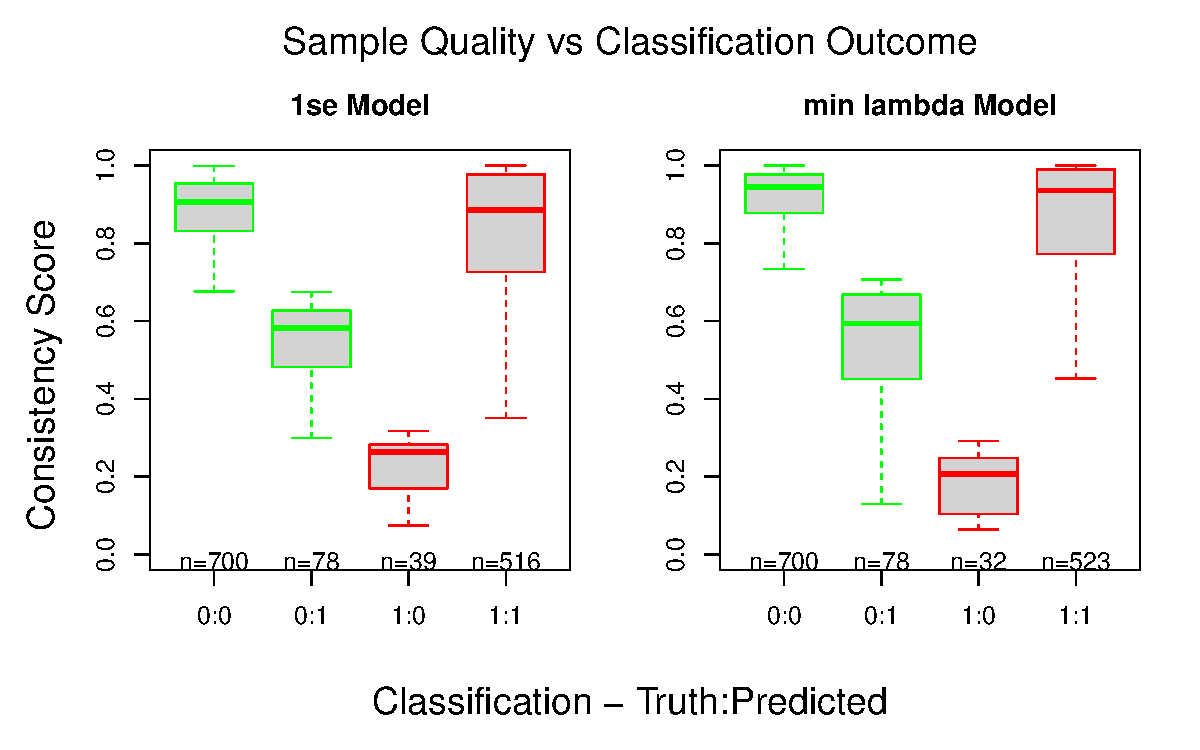
\includegraphics{Static/figures/plot-qual-conf-1.pdf}
\caption{\label{fig:plot-qual-conf}quality scores by classification - Control=0, HCC=1}
\end{figure}

This figure shows that for false positive cases (0:1 or classifying a
control as an affected case), the algorithm is \emph{less certain} of its predicted
outcome than for the fals negative cases (1:0 or classifying an affected case as a control).
ie. the misclassified HCC samples are quite similar to Controls, whereas there
is more ambiguity in the misclassified Control samples.

We will use the minimum lambda model to provide
the fitted probabilities used to compute quality scores,
but we could have used either one.

\begin{Shaded}
\begin{Highlighting}[]
\NormalTok{sample\_qual\_vec <{-}}\StringTok{ }\NormalTok{sample\_min\_qual\_vec}
\end{Highlighting}
\end{Shaded}

\hypertarget{selected-feature-list-stability}{%
\section{Selected feature list stability}\label{selected-feature-list-stability}}

Before moving on to the simulation, let's examine gene selection stability on the
full data set. We have two sets of sellected features - one for the
one standard deviation rule model, and one for the mimimum lambda model.
We saw in Table \ref{tab:model-size-lassoAll} that the number of features
selected by the minimum lambda models had an IQR of
\(175.25-261\),
while the one standard error rule models had an IQR of
\(102-132.5\).

Let's examine the stability of the gene lists across cv replicates.

\begin{Shaded}
\begin{Highlighting}[]
\CommentTok{\#\#\# CLEAR CACHE}


\CommentTok{\# 1se}
\NormalTok{lassoAll\_coef\_1se\_lst <{-}}\StringTok{ }\KeywordTok{lapply}\NormalTok{(cv\_lassoAll\_lst, }\ControlFlowTok{function}\NormalTok{(cv\_fit)\{}
\NormalTok{ cv\_fit\_coef <{-}}\StringTok{ }\KeywordTok{coef}\NormalTok{(}
\NormalTok{ cv\_fit,}
 \DataTypeTok{s =} \StringTok{"lambda.1se"}
\NormalTok{ )}
\NormalTok{ cv\_fit\_coef}\OperatorTok{@}\NormalTok{Dimnames[[}\DecValTok{1}\NormalTok{]][cv\_fit\_coef}\OperatorTok{@}\NormalTok{i[}\OperatorTok{{-}}\DecValTok{1}\NormalTok{]]}
\NormalTok{ \})}

\CommentTok{\# put into matrix}
\NormalTok{lassoAll\_coef\_1se\_all <{-}}\StringTok{ }\KeywordTok{Reduce}\NormalTok{(union, lassoAll\_coef\_1se\_lst)}
\NormalTok{lassoAll\_coef\_1se\_mtx <{-}}\StringTok{ }\KeywordTok{sapply}\NormalTok{(lassoAll\_coef\_1se\_lst, }
  \ControlFlowTok{function}\NormalTok{(LL) }\KeywordTok{is.element}\NormalTok{(lassoAll\_coef\_1se\_all, LL)}
\NormalTok{)}
\KeywordTok{rownames}\NormalTok{(lassoAll\_coef\_1se\_mtx) <{-}}\StringTok{ }\NormalTok{lassoAll\_coef\_1se\_all}

\NormalTok{genes\_by\_rep\_1se\_tbl <{-}}\StringTok{ }\KeywordTok{table}\NormalTok{(}\KeywordTok{rowSums}\NormalTok{(lassoAll\_coef\_1se\_mtx))}
\KeywordTok{barplot}\NormalTok{(}
\NormalTok{ genes\_by\_rep\_1se\_tbl,}
 \DataTypeTok{xlab=}\StringTok{\textquotesingle{}Number of Replicates\textquotesingle{}}\NormalTok{,}
 \DataTypeTok{ylab=}\StringTok{\textquotesingle{}Number of features\textquotesingle{}}

\NormalTok{)}
\end{Highlighting}
\end{Shaded}

\begin{figure}
\centering
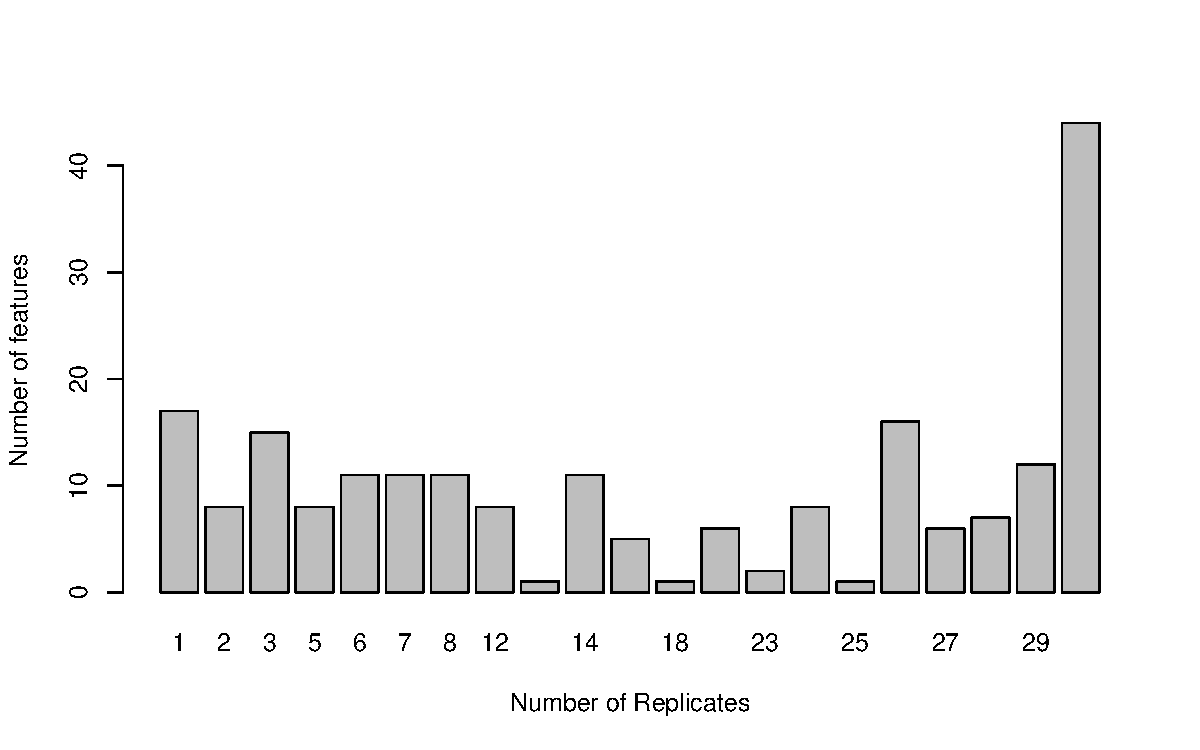
\includegraphics{Static/figures/feature-list-1se-1.pdf}
\caption{\label{fig:feature-list-1se}Feature list stability for one standard error rule models}
\end{figure}

We see that \(44\) features are included in every
cv replicate. These make up between
\(33\)\%
and
\(43\)\%
(Q1 and Q3) of the cv replicate one standard error rule models feature lists.

\begin{Shaded}
\begin{Highlighting}[]
\CommentTok{\#\#\# CLEAR CACHE}


\CommentTok{\# min}
\NormalTok{lassoAll\_coef\_min\_lst <{-}}\StringTok{ }\KeywordTok{lapply}\NormalTok{(cv\_lassoAll\_lst, }\ControlFlowTok{function}\NormalTok{(cv\_fit)\{}
\NormalTok{ cv\_fit\_coef <{-}}\StringTok{ }\KeywordTok{coef}\NormalTok{(}
\NormalTok{ cv\_fit,}
 \DataTypeTok{s =} \StringTok{"lambda.min"}
\NormalTok{ )}
\NormalTok{ cv\_fit\_coef}\OperatorTok{@}\NormalTok{Dimnames[[}\DecValTok{1}\NormalTok{]][cv\_fit\_coef}\OperatorTok{@}\NormalTok{i[}\OperatorTok{{-}}\DecValTok{1}\NormalTok{]]}
\NormalTok{ \})}

\CommentTok{\# put into matrix}
\NormalTok{lassoAll\_coef\_min\_all <{-}}\StringTok{ }\KeywordTok{Reduce}\NormalTok{(union, lassoAll\_coef\_min\_lst)}
\NormalTok{lassoAll\_coef\_min\_mtx <{-}}\StringTok{ }\KeywordTok{sapply}\NormalTok{(lassoAll\_coef\_min\_lst, }
  \ControlFlowTok{function}\NormalTok{(LL) }\KeywordTok{is.element}\NormalTok{(lassoAll\_coef\_min\_all, LL)}
\NormalTok{)}
\KeywordTok{rownames}\NormalTok{(lassoAll\_coef\_min\_mtx) <{-}}\StringTok{ }\NormalTok{lassoAll\_coef\_min\_all}

\NormalTok{genes\_by\_rep\_min\_tbl <{-}}\StringTok{ }\KeywordTok{table}\NormalTok{(}\KeywordTok{rowSums}\NormalTok{(lassoAll\_coef\_min\_mtx))}
\KeywordTok{barplot}\NormalTok{(}
\NormalTok{ genes\_by\_rep\_min\_tbl,}
 \DataTypeTok{xlab=}\StringTok{\textquotesingle{}Number of Replicates\textquotesingle{}}\NormalTok{,}
 \DataTypeTok{ylab=}\StringTok{\textquotesingle{}Number of features\textquotesingle{}}

\NormalTok{)}
\end{Highlighting}
\end{Shaded}

\begin{figure}
\centering
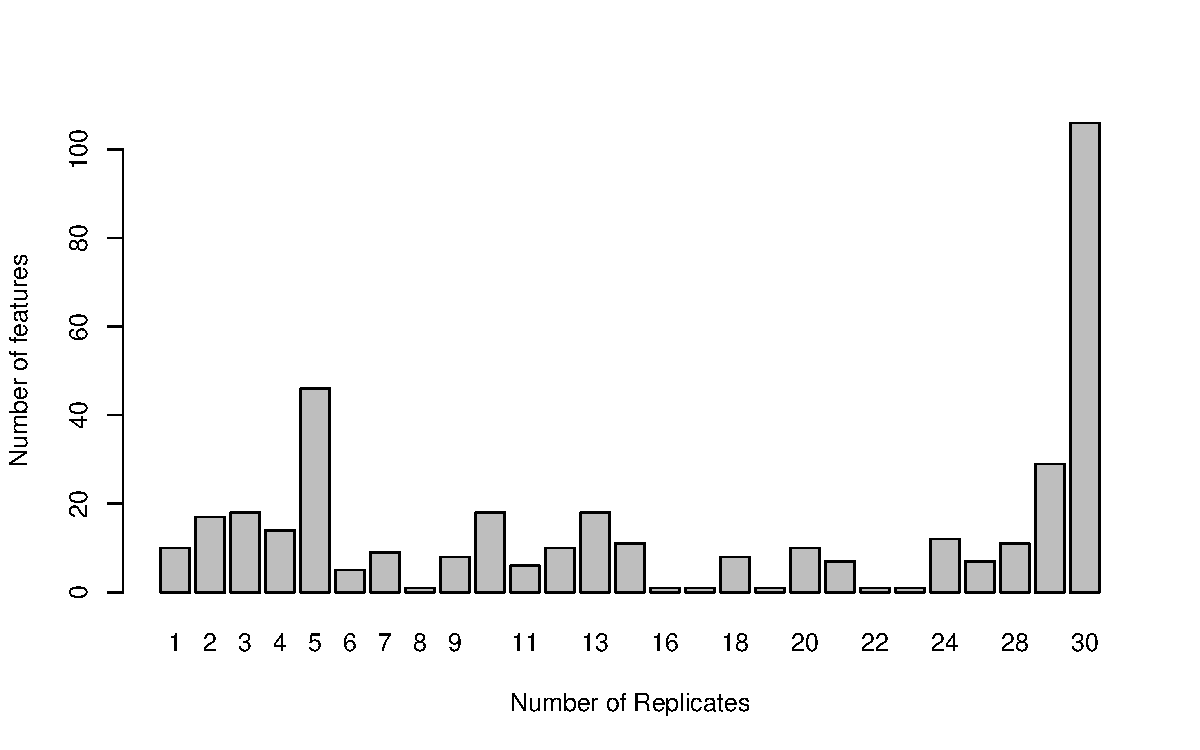
\includegraphics{Static/figures/feature-list-min-1.pdf}
\caption{\label{fig:feature-list-min}Feature list stability for minimum lambda models}
\end{figure}

We see that \(106\) features are included in every
cv replicate. These make up between
\(41\)\%
and
\(60\)\%
(Q1 and Q3) of the cv replicate min feature lists.
We will consider the genes that are selected in all cv replicates as a
gene signature produced by each model.

\begin{Shaded}
\begin{Highlighting}[]
\NormalTok{lasso\_gene\_sign\_1se\_vec <{-}}\StringTok{ }\KeywordTok{rownames}\NormalTok{(lassoAll\_coef\_1se\_mtx)[}\KeywordTok{rowSums}\NormalTok{(lassoAll\_coef\_1se\_mtx)}\OperatorTok{==}\DecValTok{30}\NormalTok{]}
\NormalTok{lasso\_gene\_sign\_min\_vec <{-}}\StringTok{ }\KeywordTok{rownames}\NormalTok{(lassoAll\_coef\_min\_mtx)[}\KeywordTok{rowSums}\NormalTok{(lassoAll\_coef\_min\_mtx)}\OperatorTok{==}\DecValTok{30}\NormalTok{]}
\end{Highlighting}
\end{Shaded}

44 out of
44 of the genes in the 1se model gene signature
are contained in the min lambda model gene signature.

\hypertarget{simulation-design}{%
\section{Simulation Design}\label{simulation-design}}

We are now ready to run the simulations.

\begin{Shaded}
\begin{Highlighting}[]
\NormalTok{ SIM <{-}}\StringTok{ }\DecValTok{30}
\NormalTok{ SIZE <{-}}\StringTok{ }\KeywordTok{c}\NormalTok{(}\DecValTok{25}\NormalTok{, }\DecValTok{50}\NormalTok{, }\DecValTok{100}\NormalTok{, }\DecValTok{200}\NormalTok{, }\DecValTok{300}\NormalTok{)}
\NormalTok{ CV\_REP <{-}}\StringTok{ }\DecValTok{30}
\end{Highlighting}
\end{Shaded}

Simluation parameters:

\begin{itemize}
\item
  Number of simulations : SIM = \(30\)
\item
  Sample sizes: SIZE = \(25, 50, 100, 200, 300\)
\item
  Number of CV Replicates: CV\_REP = \(30\)
\end{itemize}

We will repeat the simulation process SIM = \(30\) times.
For each simulation iteration, we will select \(300\) Control and
\(300\) HCC samples at random. Models will be fitted and analyzed
to balanced subsets of SIZE = \(25, 50, 100, 200, 300\), in a \texttt{Matryoshka\ doll} manner to
emulate a typical sample accrual process. Note that in this accural process
there is no time effect - the accrual process is completely randomized. In practice,
there could be significant time effects. For example, the first 25 HCC samples could come
from Center A, while the next 25 could come from Center B. And
affected and control samples could be acquired from different clinics
or in different time interevals. In other words,
there is no batch effect or shared variability in our simulation,
while these are almost always present in real data, including
batch effects that are associated with class labels - controls being in
different batches than affected samples is an all too common occurence,
for example. One should be especially watchful of potential batch effects
when dealing with blood samples as blood is notoriously finicky in
character {[}{[}\protect\hyperlink{ref-Huang:2017aa}{16}{]}; {[}\protect\hyperlink{ref-Permenter:2015aa}{17}{]};{]}.
Presented with results that look impressively good based on a small data set,
one should definitely be skeptical of the promise of future equally good results.

For a given simulation and a given sample size, we will obtain
CV\_REP = \(30\) cross-validated lasso fits. From these fits,
we can obtain \(30\) out-of-fold assessments of classification accuracy
to get a sense if its variability. From each cv replicate, we also obtain
an estimated model size and a set of selected features. We will want
to examine how these stabilize as the sample size increases.

Note that we limit the simulations to a maximum of sample size of 300 in
order to to have simulations with low overlap. With 300
randomly selected HCC samples, the expected overlap between two randomly
selected sets of HCC samples is \(29.2\)\%.
For Controls the expected overlap is \(14.9\)\%.

\hypertarget{setup-simulation}{%
\section{Setup simulation}\label{setup-simulation}}

To setup the simulation, we only need two master tables: one for the selection of Controls
and one for the selection of HCC samples.

\begin{Shaded}
\begin{Highlighting}[]
\NormalTok{all\_control\_vec <{-}}\StringTok{ }\KeywordTok{names}\NormalTok{(all\_group\_vec[all\_group\_vec}\OperatorTok{==}\StringTok{\textquotesingle{}Control\textquotesingle{}}\NormalTok{]) }
\NormalTok{all\_affected\_vec <{-}}\StringTok{ }\KeywordTok{names}\NormalTok{(all\_group\_vec[all\_group\_vec}\OperatorTok{==}\StringTok{\textquotesingle{}HCC\textquotesingle{}}\NormalTok{])  }
\end{Highlighting}
\end{Shaded}

We have \(778\) control sample IDs stored in \texttt{all\_control\_vec}
and \(555\) affected sample IDs stored in \texttt{all\_affected\_vec}.
To create a suite of random samples from these, we only need to randomly select indices from
each vector.

\begin{Shaded}
\begin{Highlighting}[]
\KeywordTok{set.seed}\NormalTok{(}\DecValTok{12379}\NormalTok{)}

\NormalTok{sim\_control\_mtx <{-}}\StringTok{ }\KeywordTok{sapply}\NormalTok{(}
 \DecValTok{1}\OperatorTok{:}\NormalTok{SIM, }
 \ControlFlowTok{function}\NormalTok{(dummy) }
   \KeywordTok{sample}\NormalTok{(}\DecValTok{1}\OperatorTok{:}\KeywordTok{length}\NormalTok{(all\_control\_vec), }\DataTypeTok{size =}  \KeywordTok{max}\NormalTok{(SIZE))}
\NormalTok{)}


\NormalTok{sim\_affected\_mtx <{-}}\StringTok{ }\KeywordTok{sapply}\NormalTok{(}
 \DecValTok{1}\OperatorTok{:}\NormalTok{SIM, }
 \ControlFlowTok{function}\NormalTok{(dummy) }
   \KeywordTok{sample}\NormalTok{(}\DecValTok{1}\OperatorTok{:}\KeywordTok{length}\NormalTok{(all\_affected\_vec), }\DataTypeTok{size =}  \KeywordTok{max}\NormalTok{(SIZE))}
\NormalTok{)}
\end{Highlighting}
\end{Shaded}

Each simulation is specified by a given column of the simulation design matrices:
\texttt{sim\_control\_mtx} and \texttt{sim\_affected\_mtx}, each with domensions \(300, 30\).
Within each simulation, we can run the analyses of size \(25, 50, 100, 200, 300\) by simply selecting
samples specified in the appropriate rows of each design matrix.

We can examine how much variability we have in the quality scores of the selected samples.
Here we show results for the smalle sample sizes where variability will be the greatest.

\begin{Shaded}
\begin{Highlighting}[]
\CommentTok{\#\#\# CLEAR CACHE}

\NormalTok{all\_control\_qual\_vec <{-}}\StringTok{ }\NormalTok{sample\_qual\_vec[all\_control\_vec]}
\NormalTok{sim\_control\_qual\_mtx <{-}}\StringTok{ }\KeywordTok{sapply}\NormalTok{(}
  \DecValTok{1}\OperatorTok{:}\KeywordTok{ncol}\NormalTok{(sim\_control\_mtx), }
  \ControlFlowTok{function}\NormalTok{(CC) all\_control\_qual\_vec[sim\_control\_mtx[,CC]]}
\NormalTok{ )}

\NormalTok{all\_affected\_qual\_vec <{-}}\StringTok{ }\NormalTok{sample\_qual\_vec[all\_affected\_vec]}
\NormalTok{sim\_affected\_qual\_mtx <{-}}\StringTok{ }\KeywordTok{sapply}\NormalTok{(}
  \DecValTok{1}\OperatorTok{:}\KeywordTok{ncol}\NormalTok{(sim\_affected\_mtx),  }
  \ControlFlowTok{function}\NormalTok{(CC) all\_affected\_qual\_vec[sim\_affected\_mtx[,CC]]}
\NormalTok{ )}

\CommentTok{\# ONLY LOOK AT SAMPLE SIZE == 50}
\NormalTok{NN <{-}}\StringTok{ }\DecValTok{50}

\CommentTok{\# PLOT}
\KeywordTok{par}\NormalTok{(}\DataTypeTok{mfrow=}\KeywordTok{c}\NormalTok{(}\DecValTok{2}\NormalTok{,}\DecValTok{1}\NormalTok{), }\DataTypeTok{mar =} \KeywordTok{c}\NormalTok{(}\DecValTok{2}\NormalTok{,}\DecValTok{5}\NormalTok{,}\DecValTok{2}\NormalTok{,}\DecValTok{1}\NormalTok{))}
\CommentTok{\# control}
\KeywordTok{boxplot}\NormalTok{(}
\NormalTok{  sim\_control\_qual\_mtx[}\DecValTok{1}\OperatorTok{:}\NormalTok{NN,],}
  \DataTypeTok{outline =}\NormalTok{ T, }
  \DataTypeTok{ylab =} \StringTok{\textquotesingle{}Quality Score\textquotesingle{}}\NormalTok{,}
  \DataTypeTok{xaxt =} \StringTok{\textquotesingle{}n\textquotesingle{}}
\NormalTok{)}
\KeywordTok{title}\NormalTok{(}\StringTok{"Control sample quality across simulations"}\NormalTok{)}

\CommentTok{\# affected}
\KeywordTok{boxplot}\NormalTok{(}
\NormalTok{  sim\_affected\_qual\_mtx[}\DecValTok{1}\OperatorTok{:}\NormalTok{NN,],}
  \DataTypeTok{outline =}\NormalTok{ T, }
  \DataTypeTok{ylab =} \StringTok{\textquotesingle{}Quality Score\textquotesingle{}}
\NormalTok{)}
\KeywordTok{title}\NormalTok{(}\StringTok{"Affected sample quality across simulations"}\NormalTok{)}
\end{Highlighting}
\end{Shaded}

\begin{figure}
\centering
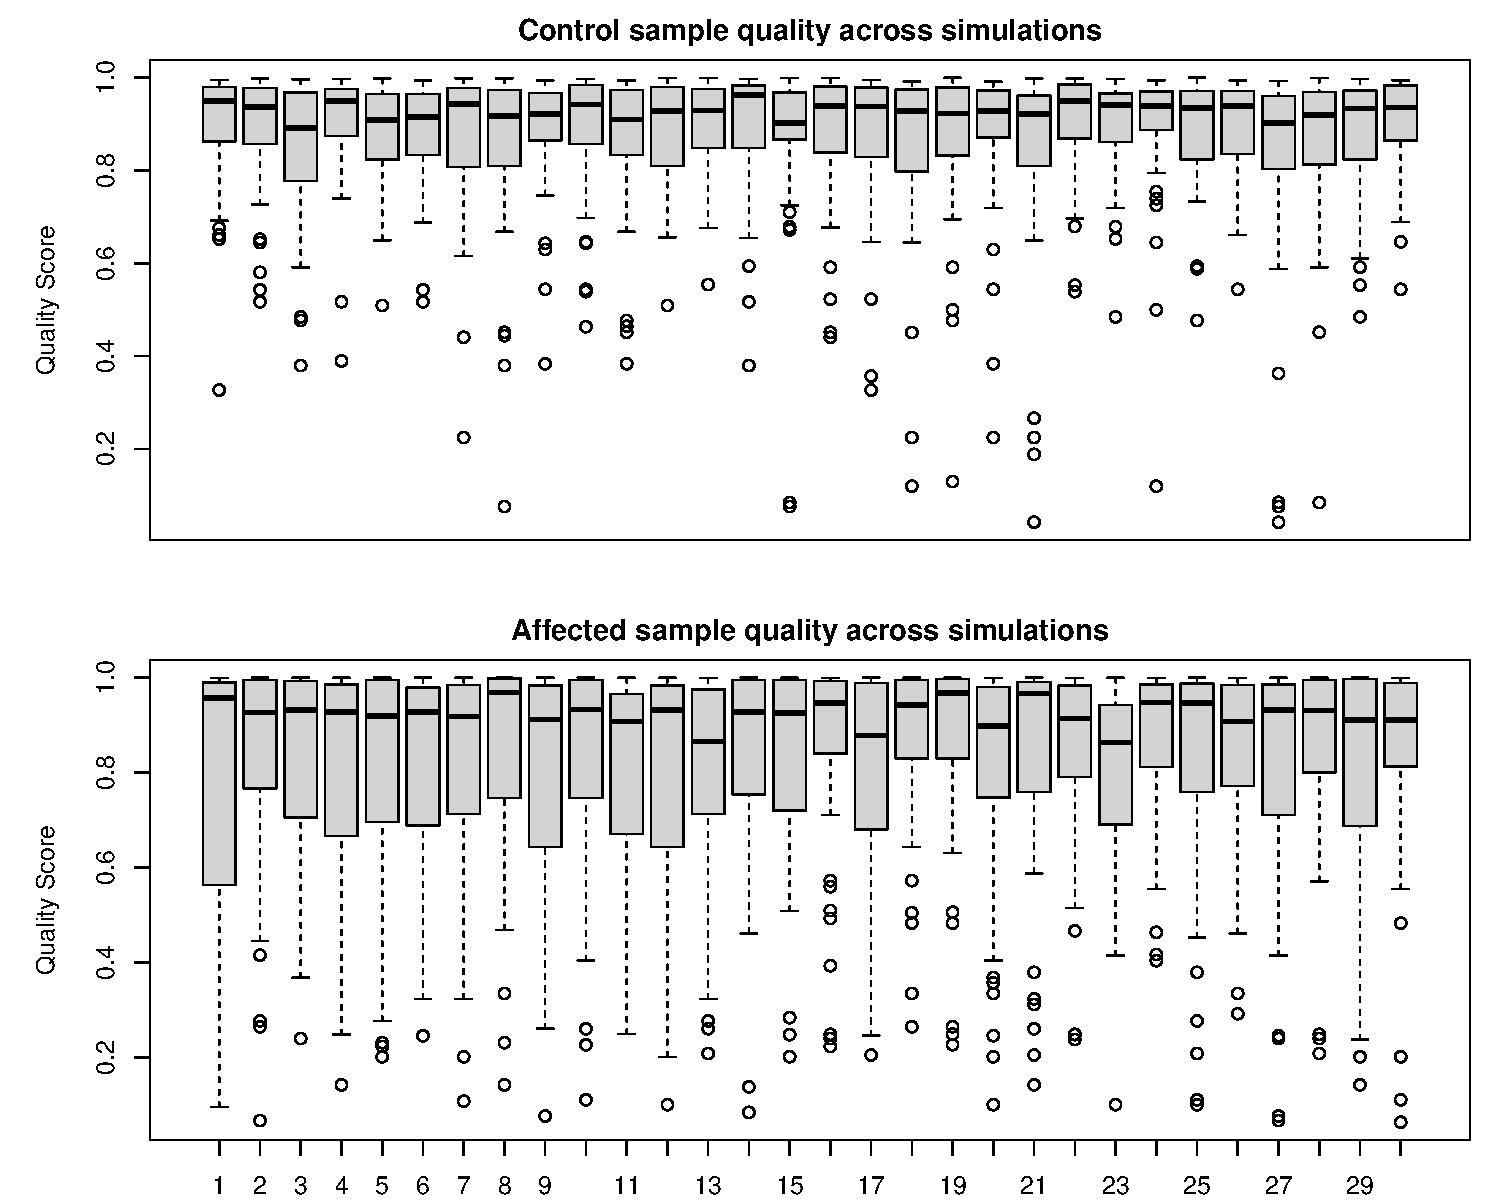
\includegraphics{Static/figures/look-sim-qual-0-50ONLY-1.pdf}
\caption{\label{fig:look-sim-qual-0-50ONLY}sample quality by simulation run for size = 50}
\end{figure}

In this figure, we are summarizing the quality measures of 50 samples per group acress
30 simulations, or random selections of control and affected samples.
We see significant variability in sample quality, especially in the affected cases.
This may lead an unwary observer to be overly optimistic, or overly pessimistic,
in the early accrual stages of a study.

\hypertarget{run-simulations}{%
\section{Run simulations}\label{run-simulations}}

As these take a while to run,
we will save the results of each similation to a different
object and store to disk. These can be easily read from disk
when needed for analysis.

The simulation results are saved to the file system and
only needs to be run once. The simulation takes \(\approx\) 8 to 10 minutes
per iteration, or 4 to 5 hours of run time on a laptop.
(Platform: x86\_64-apple-darwin17.0 (64-bit)
Running under: macOS Mojave 10.14.6)

\begin{Shaded}
\begin{Highlighting}[]
\NormalTok{start\_time <{-}}\StringTok{ }\KeywordTok{proc.time}\NormalTok{()}

\CommentTok{\# Get stage from SIZE}
\NormalTok{stage\_vec <{-}}\StringTok{ }\KeywordTok{cut}\NormalTok{(}\DecValTok{1}\OperatorTok{:}\KeywordTok{nrow}\NormalTok{(sim\_control\_qual\_mtx), }\KeywordTok{c}\NormalTok{(}\DecValTok{0}\NormalTok{, SIZE), }\DataTypeTok{include.lowest =}\NormalTok{ T)}

\ControlFlowTok{for}\NormalTok{ (SIMno }\ControlFlowTok{in} \DecValTok{1}\OperatorTok{:}\KeywordTok{ncol}\NormalTok{(sim\_control\_qual\_mtx)) \{}

  \CommentTok{\#cat("Running simulation ", SIMno, "\textbackslash{}n")}

\NormalTok{  sim\_cv\_lst <{-}}\StringTok{ }\KeywordTok{lapply}\NormalTok{(}\DecValTok{1}\OperatorTok{:}\KeywordTok{length}\NormalTok{(}\KeywordTok{levels}\NormalTok{(stage\_vec)), }\ControlFlowTok{function}\NormalTok{(STGno) \{}
\NormalTok{    Stage\_rows\_vec <{-}}\StringTok{ }\KeywordTok{which}\NormalTok{(stage\_vec }\OperatorTok{\%in\%}\StringTok{ }\KeywordTok{levels}\NormalTok{(stage\_vec)[}\DecValTok{1}\OperatorTok{:}\NormalTok{STGno])}
    \CommentTok{\#cat("Stage ", STGno, "{-} analyzing", length(Stage\_rows\_vec), "paired samples.\textbackslash{}n")}

\NormalTok{    sim\_stage\_samples\_vec <{-}}\StringTok{ }\KeywordTok{c}\NormalTok{(}
\NormalTok{      all\_control\_vec[sim\_control\_mtx[Stage\_rows\_vec, SIMno]],}
\NormalTok{      all\_affected\_vec[sim\_affected\_mtx[Stage\_rows\_vec, SIMno]]}
\NormalTok{    )}
\NormalTok{    sim\_stage\_lcpm\_mtx <{-}}\StringTok{ }\NormalTok{all\_lcpm\_mtx[sim\_stage\_samples\_vec, ]}
\NormalTok{    sim\_stage\_group\_vec <{-}}\StringTok{ }\NormalTok{all\_group\_vec[sim\_stage\_samples\_vec]}
    \CommentTok{\#print(table(sim\_stage\_group\_vec))}

\NormalTok{    sim\_stage\_cv\_lst <{-}}\StringTok{ }\KeywordTok{lapply}\NormalTok{(}\DecValTok{1}\OperatorTok{:}\NormalTok{CV\_REP, }\ControlFlowTok{function}\NormalTok{(CV) \{}
\NormalTok{      cv\_fit <{-}}\StringTok{ }\NormalTok{glmnet}\OperatorTok{::}\KeywordTok{cv.glmnet}\NormalTok{(}
        \DataTypeTok{x =}\NormalTok{ sim\_stage\_lcpm\_mtx,}
        \DataTypeTok{y =}\NormalTok{ sim\_stage\_group\_vec,}
        \DataTypeTok{alpha =} \DecValTok{1}\NormalTok{,}
        \DataTypeTok{family =} \StringTok{"binomial"}\NormalTok{,}
        \DataTypeTok{type.measure =} \StringTok{"class"}\NormalTok{,}
        \DataTypeTok{keep =}\NormalTok{ T,}
        \DataTypeTok{nlambda =} \DecValTok{30}
\NormalTok{      )}

      \CommentTok{\# Extract 1se metrics from cv\_fit}
      \CommentTok{\#\#\#\#\#\#\#\#\#\#\#\#\#\#\#\#\#\#\#\#\#\#\#}
\NormalTok{      ndx\_1se <{-}}\StringTok{ }\KeywordTok{which}\NormalTok{(cv\_fit}\OperatorTok{$}\NormalTok{lambda }\OperatorTok{==}\StringTok{ }\NormalTok{cv\_fit}\OperatorTok{$}\NormalTok{lambda}\FloatTok{.1}\NormalTok{se)}

\NormalTok{      nzero\_1se <{-}}\StringTok{ }\NormalTok{cv\_fit}\OperatorTok{$}\NormalTok{nzero[ndx\_1se]}
\NormalTok{      cvm\_1se <{-}}\StringTok{ }\NormalTok{cv\_fit}\OperatorTok{$}\NormalTok{cvm[ndx\_1se]}

      \CommentTok{\# test error}
\NormalTok{      sim\_stage\_test\_samples\_vec <{-}}\StringTok{ }\KeywordTok{setdiff}\NormalTok{(}\KeywordTok{rownames}\NormalTok{(all\_lcpm\_mtx), sim\_stage\_samples\_vec)}
\NormalTok{      sim\_stage\_test\_lcpm\_mtx <{-}}\StringTok{ }\NormalTok{all\_lcpm\_mtx[sim\_stage\_test\_samples\_vec,]}
\NormalTok{      sim\_stage\_test\_group\_vec <{-}}\StringTok{ }\NormalTok{all\_group\_vec[sim\_stage\_test\_samples\_vec]}

\NormalTok{      test\_pred\_1se\_vec <{-}}\StringTok{ }\KeywordTok{predict}\NormalTok{(}
\NormalTok{       cv\_fit,}
       \DataTypeTok{newx=}\NormalTok{sim\_stage\_test\_lcpm\_mtx,}
       \DataTypeTok{s=}\StringTok{"lambda.1se"}\NormalTok{,}
       \DataTypeTok{type=}\StringTok{"class"}
\NormalTok{      )}
\NormalTok{      test\_1se\_error <{-}}\StringTok{ }\KeywordTok{mean}\NormalTok{(test\_pred\_1se\_vec }\OperatorTok{!=}\StringTok{ }\NormalTok{sim\_stage\_test\_group\_vec)}

      \CommentTok{\# genes}
\NormalTok{      coef\_1se <{-}}\StringTok{ }\KeywordTok{coef}\NormalTok{(}
\NormalTok{        cv\_fit,}
        \DataTypeTok{s =} \StringTok{"lambda.1se"}
\NormalTok{      )}
\NormalTok{      genes\_1se <{-}}\StringTok{ }\NormalTok{coef\_1se}\OperatorTok{@}\NormalTok{Dimnames[[}\DecValTok{1}\NormalTok{]][coef\_1se}\OperatorTok{@}\NormalTok{i[}\OperatorTok{{-}}\DecValTok{1}\NormalTok{]]}

      \CommentTok{\# Extract min metrics from cv\_fit}
      \CommentTok{\#\#\#\#\#\#\#\#\#\#\#\#\#\#\#\#\#\#\#\#\#\#\#}
\NormalTok{      ndx\_min <{-}}\StringTok{ }\KeywordTok{which}\NormalTok{(cv\_fit}\OperatorTok{$}\NormalTok{lambda }\OperatorTok{==}\StringTok{ }\NormalTok{cv\_fit}\OperatorTok{$}\NormalTok{lambda.min)}

\NormalTok{      nzero\_min <{-}}\StringTok{ }\NormalTok{cv\_fit}\OperatorTok{$}\NormalTok{nzero[ndx\_min]}
\NormalTok{      cvm\_min <{-}}\StringTok{ }\NormalTok{cv\_fit}\OperatorTok{$}\NormalTok{cvm[ndx\_min]}

      \CommentTok{\# test error}
\NormalTok{      sim\_stage\_test\_samples\_vec <{-}}\StringTok{ }\KeywordTok{setdiff}\NormalTok{(}\KeywordTok{rownames}\NormalTok{(all\_lcpm\_mtx), sim\_stage\_samples\_vec)}
\NormalTok{      sim\_stage\_test\_lcpm\_mtx <{-}}\StringTok{ }\NormalTok{all\_lcpm\_mtx[sim\_stage\_test\_samples\_vec,]}
\NormalTok{      sim\_stage\_test\_group\_vec <{-}}\StringTok{ }\NormalTok{all\_group\_vec[sim\_stage\_test\_samples\_vec]}

\NormalTok{      test\_pred\_min\_vec <{-}}\StringTok{ }\KeywordTok{predict}\NormalTok{(}
\NormalTok{       cv\_fit,}
       \DataTypeTok{newx=}\NormalTok{sim\_stage\_test\_lcpm\_mtx,}
       \DataTypeTok{s=}\StringTok{"lambda.min"}\NormalTok{,}
       \DataTypeTok{type=}\StringTok{"class"}
\NormalTok{      )}
\NormalTok{      test\_min\_error <{-}}\StringTok{ }\KeywordTok{mean}\NormalTok{(test\_pred\_min\_vec }\OperatorTok{!=}\StringTok{ }\NormalTok{sim\_stage\_test\_group\_vec)}

      \CommentTok{\# genes}
\NormalTok{      coef\_min <{-}}\StringTok{ }\KeywordTok{coef}\NormalTok{(}
\NormalTok{        cv\_fit,}
        \DataTypeTok{s =} \StringTok{"lambda.min"}
\NormalTok{      )}
\NormalTok{      genes\_min <{-}}\StringTok{ }\NormalTok{coef\_min}\OperatorTok{@}\NormalTok{Dimnames[[}\DecValTok{1}\NormalTok{]][coef\_min}\OperatorTok{@}\NormalTok{i[}\OperatorTok{{-}}\DecValTok{1}\NormalTok{]]}

      \CommentTok{\# return cv\_fit summary metrics}
      \KeywordTok{list}\NormalTok{(}
       \DataTypeTok{p\_1se =}\NormalTok{ nzero\_1se, }
       \DataTypeTok{p\_min =}\NormalTok{ nzero\_min, }
       \DataTypeTok{cv\_1se =}\NormalTok{ cvm\_1se, }
       \DataTypeTok{cv\_min =}\NormalTok{ cvm\_min, }
       \DataTypeTok{test\_1se=}\NormalTok{test\_1se\_error, }
       \DataTypeTok{test\_min=}\NormalTok{test\_min\_error, }
       \DataTypeTok{genes\_1se =}\NormalTok{ genes\_1se,}
       \DataTypeTok{genes\_min =}\NormalTok{ genes\_min)}
\NormalTok{    \})}
\NormalTok{    sim\_stage\_cv\_lst}
\NormalTok{  \})}

  \CommentTok{\# save  sim\_cv\_lst}
\NormalTok{  fName <{-}}\StringTok{ }\KeywordTok{paste0}\NormalTok{(}\StringTok{"sim\_"}\NormalTok{, SIMno, }\StringTok{"\_cv\_lst"}\NormalTok{)}
  \KeywordTok{assign}\NormalTok{(fName, sim\_cv\_lst)}
  \KeywordTok{save}\NormalTok{(}\DataTypeTok{list =}\NormalTok{ fName, }\DataTypeTok{file=}\KeywordTok{file.path}\NormalTok{(}\StringTok{"RData"}\NormalTok{, fName))}

\NormalTok{\}}
\end{Highlighting}
\end{Shaded}

\hypertarget{simulation-results}{%
\section{Simulation results}\label{simulation-results}}

Recall the we have \(30\) simulations, or randomly selected sets of HCC and Control samples,
analyzed in inreasing sizes of \(25, 50, 100, 200, 300\), with
\(30\) repeated cross-validated lasso fits:

\begin{itemize}
\item
  Sample sizes: SIZE = \(25, 50, 100, 200, 300\)
\item
  Number of CV Replicates: CV\_REP = \(30\)
\end{itemize}

First we extract simluation results and store into one big table (only showing the top of table shere):

\begin{Shaded}
\begin{Highlighting}[]
\CommentTok{\#\#\# CLEAR CACHE}
\NormalTok{sim\_files\_vec <{-}}\StringTok{ }\KeywordTok{list.files}\NormalTok{(}\StringTok{\textquotesingle{}RData\textquotesingle{}}\NormalTok{, }\StringTok{\textquotesingle{}\^{}sim\_\textquotesingle{}}\NormalTok{)}


\CommentTok{\# define extraction methods}

\CommentTok{\# Each sumulation is a list of cv results }
\CommentTok{\#\# nested in a list of replicates}
\CommentTok{\#\#\#\#\#\#\#\#\#\#\#\#\#\#\#\#\#\#\#\#\#\#\#\#\#\#\#\#\#\#\#\#\#\#\#\#\#\#\#\#\#\#\#\#\#\#}

\CommentTok{\# cvList2frm\_f makes a frame out of the inner list}
\NormalTok{cvList2frm\_f <{-}}\StringTok{ }\ControlFlowTok{function}\NormalTok{(cv\_lst) \{}
\NormalTok{ frm1 <{-}}\StringTok{ }\KeywordTok{as.data.frame}\NormalTok{(}\KeywordTok{t}\NormalTok{(}\KeywordTok{sapply}\NormalTok{(cv\_lst, }\ControlFlowTok{function}\NormalTok{(x) x)))}
\NormalTok{ frm2 <{-}}\StringTok{ }\KeywordTok{data.frame}\NormalTok{(}
  \KeywordTok{unlist}\NormalTok{(frm1[[}\DecValTok{1}\NormalTok{]]), }\KeywordTok{unlist}\NormalTok{(frm1[[}\DecValTok{2}\NormalTok{]]),}
  \KeywordTok{unlist}\NormalTok{(frm1[[}\DecValTok{3}\NormalTok{]]), }\KeywordTok{unlist}\NormalTok{(frm1[[}\DecValTok{4}\NormalTok{]]),}
  \KeywordTok{unlist}\NormalTok{(frm1[[}\DecValTok{5}\NormalTok{]]), }\KeywordTok{unlist}\NormalTok{(frm1[[}\DecValTok{6}\NormalTok{]]),}
\NormalTok{  frm1[}\DecValTok{7}\NormalTok{], frm1[}\DecValTok{8}\NormalTok{])}
  \KeywordTok{names}\NormalTok{(frm2) <{-}}\StringTok{ }\KeywordTok{names}\NormalTok{(frm1)}
  \KeywordTok{data.frame}\NormalTok{(}\DataTypeTok{Rep=}\DecValTok{1}\OperatorTok{:}\KeywordTok{nrow}\NormalTok{(frm2), frm2)\}}

\CommentTok{\# cv\_lst\_to\_frm loop over replicates, concatenating the inner list frames}
\NormalTok{cv\_lst\_to\_frm <{-}}\StringTok{ }\ControlFlowTok{function}\NormalTok{(sim\_cv\_lst) \{}
 \KeywordTok{do.call}\NormalTok{(}\StringTok{\textquotesingle{}rbind\textquotesingle{}}\NormalTok{, }\KeywordTok{lapply}\NormalTok{(}\DecValTok{1}\OperatorTok{:}\KeywordTok{length}\NormalTok{(sim\_cv\_lst),}
  \ControlFlowTok{function}\NormalTok{(JJ) \{}
\NormalTok{    siz\_frm <{-}}\StringTok{ }\KeywordTok{cvList2frm\_f}\NormalTok{(sim\_cv\_lst[[JJ]])}
    \KeywordTok{data.frame}\NormalTok{(}\DataTypeTok{Size=}\NormalTok{SIZE[JJ], siz\_frm)}
\NormalTok{  \}))}
\NormalTok{\}}

\CommentTok{\# we loop across simulations to combine all results into one big table}
\NormalTok{lasso\_sim\_results\_frm <{-}}\StringTok{ }\KeywordTok{do.call}\NormalTok{(}\StringTok{\textquotesingle{}rbind\textquotesingle{}}\NormalTok{, }\KeywordTok{lapply}\NormalTok{(}\DecValTok{1}\OperatorTok{:}\KeywordTok{length}\NormalTok{(sim\_files\_vec),}
 \ControlFlowTok{function}\NormalTok{(SIM\_NO) \{}
  \KeywordTok{load}\NormalTok{(}\DataTypeTok{file=}\KeywordTok{file.path}\NormalTok{(}\StringTok{\textquotesingle{}RData\textquotesingle{}}\NormalTok{, sim\_files\_vec[SIM\_NO]))}
  \KeywordTok{assign}\NormalTok{(}\StringTok{\textquotesingle{}sim\_cv\_lst\textquotesingle{}}\NormalTok{, }\KeywordTok{get}\NormalTok{(sim\_files\_vec[SIM\_NO]))}
  \KeywordTok{rm}\NormalTok{(}\DataTypeTok{list=}\NormalTok{sim\_files\_vec[SIM\_NO])}
  
  \KeywordTok{data.frame}\NormalTok{(}\DataTypeTok{SimNo=}\KeywordTok{paste0}\NormalTok{(}\StringTok{\textquotesingle{}Sim\_\textquotesingle{}}\NormalTok{,}\KeywordTok{formatC}\NormalTok{(SIM\_NO,}\DataTypeTok{width =} \DecValTok{2}\NormalTok{,}\DataTypeTok{flag =} \DecValTok{0}\NormalTok{)), }\KeywordTok{cv\_lst\_to\_frm}\NormalTok{(sim\_cv\_lst))}
\NormalTok{\} }
\NormalTok{)) }
\end{Highlighting}
\end{Shaded}

\begin{Shaded}
\begin{Highlighting}[]
\CommentTok{\#\#\# CLEAR CACHE}
 
\NormalTok{knitr}\OperatorTok{::}\KeywordTok{kable}\NormalTok{(}\KeywordTok{head}\NormalTok{(}\KeywordTok{with}\NormalTok{(lasso\_sim\_results\_frm, }\KeywordTok{table}\NormalTok{(SimNo, Size))),}
  \DataTypeTok{caption =} \KeywordTok{paste}\NormalTok{(}\StringTok{"Simulation Results {-} N Sim ="}\NormalTok{, SIM)) }\OperatorTok{\%>\%}
\StringTok{   }\NormalTok{kableExtra}\OperatorTok{::}\KeywordTok{kable\_styling}\NormalTok{(}\DataTypeTok{full\_width =}\NormalTok{ F)}
\end{Highlighting}
\end{Shaded}

\begin{table}

\caption{\label{tab:sum-table}Simulation Results - N Sim = 30}
\centering
\begin{tabular}[t]{l|r|r|r|r|r}
\hline
  & 25 & 50 & 100 & 200 & 300\\
\hline
Sim\_01 & 30 & 30 & 30 & 30 & 30\\
\hline
Sim\_02 & 30 & 30 & 30 & 30 & 30\\
\hline
Sim\_03 & 30 & 30 & 30 & 30 & 30\\
\hline
Sim\_04 & 30 & 30 & 30 & 30 & 30\\
\hline
Sim\_05 & 30 & 30 & 30 & 30 & 30\\
\hline
Sim\_06 & 30 & 30 & 30 & 30 & 30\\
\hline
\end{tabular}
\end{table}

\begin{Shaded}
\begin{Highlighting}[]
\NormalTok{knitr}\OperatorTok{::}\KeywordTok{kable}\NormalTok{(}\KeywordTok{head}\NormalTok{(lasso\_sim\_results\_frm) }\OperatorTok{\%>\%}\StringTok{ }\NormalTok{dplyr}\OperatorTok{::}\KeywordTok{select}\NormalTok{(}\OperatorTok{{-}}\KeywordTok{c}\NormalTok{(genes\_1se, genes\_min)),}
    \DataTypeTok{caption =} \KeywordTok{paste}\NormalTok{(}\StringTok{"Simulation Results {-} not showing genes column"}\NormalTok{),}
    \DataTypeTok{digits=}\DecValTok{2}\NormalTok{) }\OperatorTok{\%>\%}
\StringTok{   }\NormalTok{kableExtra}\OperatorTok{::}\KeywordTok{kable\_styling}\NormalTok{(}\DataTypeTok{full\_width =}\NormalTok{ F)}
\end{Highlighting}
\end{Shaded}

\begin{table}

\caption{\label{tab:sum-table}Simulation Results - not showing genes column}
\centering
\begin{tabular}[t]{l|r|r|r|r|r|r|r|r}
\hline
SimNo & Size & Rep & p\_1se & p\_min & cv\_1se & cv\_min & test\_1se & test\_min\\
\hline
Sim\_01 & 25 & 1 & 20 & 40 & 0.32 & 0.26 & 0.30 & 0.31\\
\hline
Sim\_01 & 25 & 2 & 26 & 26 & 0.22 & 0.22 & 0.29 & 0.29\\
\hline
Sim\_01 & 25 & 3 & 6 & 32 & 0.34 & 0.30 & 0.35 & 0.31\\
\hline
Sim\_01 & 25 & 4 & 10 & 24 & 0.36 & 0.30 & 0.32 & 0.29\\
\hline
Sim\_01 & 25 & 5 & 27 & 32 & 0.26 & 0.22 & 0.30 & 0.31\\
\hline
Sim\_01 & 25 & 6 & 20 & 27 & 0.36 & 0.32 & 0.30 & 0.30\\
\hline
\end{tabular}
\end{table}

\hypertarget{simulation-results---look-at-one-simulation}{%
\subsection{Simulation Results - look at one simulation}\label{simulation-results---look-at-one-simulation}}

First examine results for one simulation run. In the figures that follow,
each boxplot summarized 30 repreated cross validation runs performed on a
fixed random selection of Control and Affeced samples. Recall that as
we move from 25 to 50, etc., the sample sets are growing to emulate an
accrual of samples over time.

\begin{Shaded}
\begin{Highlighting}[]
\CommentTok{\#\#\# CLEAR CACHE}

\CommentTok{\# get full model cv error ref}
\NormalTok{error\_1se\_vec <{-}}\StringTok{ }\KeywordTok{sapply}\NormalTok{(cv\_lassoAll\_lst,}
 \ControlFlowTok{function}\NormalTok{(cv\_fit) cv\_fit}\OperatorTok{$}\NormalTok{cvm[cv\_fit}\OperatorTok{$}\NormalTok{lambda }\OperatorTok{==}\StringTok{ }\NormalTok{cv\_fit}\OperatorTok{$}\NormalTok{lambda}\FloatTok{.1}\NormalTok{se])}
\NormalTok{error\_1se\_q2 <{-}}\StringTok{ }\KeywordTok{quantile}\NormalTok{(error\_1se\_vec, }\DataTypeTok{prob=}\DecValTok{1}\OperatorTok{/}\DecValTok{2}\NormalTok{)        }

\NormalTok{error\_min\_vec <{-}}\StringTok{ }\KeywordTok{sapply}\NormalTok{(cv\_lassoAll\_lst,}
 \ControlFlowTok{function}\NormalTok{(cv\_fit) cv\_fit}\OperatorTok{$}\NormalTok{cvm[cv\_fit}\OperatorTok{$}\NormalTok{lambda }\OperatorTok{==}\StringTok{ }\NormalTok{cv\_fit}\OperatorTok{$}\NormalTok{lambda.min])}
\NormalTok{error\_min\_q2 <{-}}\StringTok{ }\KeywordTok{quantile}\NormalTok{(error\_min\_vec, }\DataTypeTok{prob=}\DecValTok{1}\OperatorTok{/}\DecValTok{2}\NormalTok{)        }

\CommentTok{\# Utility objects}
\NormalTok{SIZE0 <{-}}\StringTok{ }\NormalTok{stringr}\OperatorTok{::}\KeywordTok{str\_pad}\NormalTok{(SIZE, }\DataTypeTok{width=}\DecValTok{3}\NormalTok{, }\DataTypeTok{pad=}\StringTok{\textquotesingle{}0\textquotesingle{}}\NormalTok{)}
\NormalTok{stage\_vec <{-}}\StringTok{ }\KeywordTok{cut}\NormalTok{(}\DecValTok{1}\OperatorTok{:}\KeywordTok{nrow}\NormalTok{(sim\_control\_qual\_mtx), }\KeywordTok{c}\NormalTok{(}\DecValTok{0}\NormalTok{,SIZE), }\DataTypeTok{include.lowest =}\NormalTok{ T)}


\CommentTok{\#SIM <{-} "Sim\_01"}

\ControlFlowTok{for}\NormalTok{(SIM }\ControlFlowTok{in} \KeywordTok{unique}\NormalTok{(lasso\_sim\_results\_frm}\OperatorTok{$}\NormalTok{SimNo)[}\DecValTok{1}\NormalTok{])\{}

\NormalTok{SimNum <{-}}\StringTok{ }\KeywordTok{as.numeric}\NormalTok{(}\KeywordTok{sub}\NormalTok{(}\StringTok{\textquotesingle{}Sim\_\textquotesingle{}}\NormalTok{,}\StringTok{\textquotesingle{}\textquotesingle{}}\NormalTok{,SIM))}

\NormalTok{simNo\_results\_frm <{-}}\StringTok{ }\NormalTok{lasso\_sim\_results\_frm }\OperatorTok{\%>\%}\StringTok{ }\NormalTok{dplyr}\OperatorTok{::}\KeywordTok{filter}\NormalTok{(SimNo}\OperatorTok{==}\NormalTok{SIM)}


\CommentTok{\# errors}
\KeywordTok{par}\NormalTok{(}\DataTypeTok{mfrow=}\KeywordTok{c}\NormalTok{(}\DecValTok{1}\NormalTok{,}\DecValTok{2}\NormalTok{), }\DataTypeTok{mar=}\KeywordTok{c}\NormalTok{(}\DecValTok{4}\NormalTok{, }\DecValTok{2}\NormalTok{, }\DecValTok{2}\NormalTok{, }\DecValTok{1}\NormalTok{), }\DataTypeTok{oma=}\KeywordTok{c}\NormalTok{(}\DecValTok{0}\NormalTok{,}\DecValTok{0}\NormalTok{,}\DecValTok{2}\NormalTok{,}\DecValTok{0}\NormalTok{))}
\CommentTok{\#\#\#\#\#\#\#\#\#\#\#\#\#\#\#\#\#\#\#}
\CommentTok{\# 1se}
\CommentTok{\#\#\#\#\#\#\#\#\#\#\#\#\#\#\#\#\#\#\#\#}
\NormalTok{cv\_1se\_lst <{-}}\StringTok{ }\KeywordTok{with}\NormalTok{(simNo\_results\_frm,}
 \KeywordTok{split}\NormalTok{(cv\_1se, Size))}
\KeywordTok{names}\NormalTok{(cv\_1se\_lst) <{-}}\StringTok{ }\KeywordTok{paste0}\NormalTok{(stringr}\OperatorTok{::}\KeywordTok{str\_pad}\NormalTok{(}\KeywordTok{names}\NormalTok{(cv\_1se\_lst), }\DataTypeTok{width=}\DecValTok{3}\NormalTok{, }\DataTypeTok{pad=}\StringTok{\textquotesingle{}0\textquotesingle{}}\NormalTok{),}\StringTok{\textquotesingle{}\_cv\textquotesingle{}}\NormalTok{)}

\NormalTok{test\_1se\_lst <{-}}\StringTok{ }\KeywordTok{with}\NormalTok{(simNo\_results\_frm,}
 \KeywordTok{split}\NormalTok{(test\_1se, Size))}
\KeywordTok{names}\NormalTok{(test\_1se\_lst) <{-}}\StringTok{ }\KeywordTok{paste0}\NormalTok{(stringr}\OperatorTok{::}\KeywordTok{str\_pad}\NormalTok{(}\KeywordTok{names}\NormalTok{(test\_1se\_lst), }\DataTypeTok{width=}\DecValTok{3}\NormalTok{, }\DataTypeTok{pad=}\StringTok{\textquotesingle{}0\textquotesingle{}}\NormalTok{),}\StringTok{\textquotesingle{}\_cv\textquotesingle{}}\NormalTok{)}

\NormalTok{error\_1se\_lst <{-}}\StringTok{ }\KeywordTok{c}\NormalTok{(cv\_1se\_lst, test\_1se\_lst)}
\NormalTok{error\_1se\_lst <{-}}\StringTok{ }\NormalTok{error\_1se\_lst[}\KeywordTok{order}\NormalTok{(}\KeywordTok{names}\NormalTok{(error\_1se\_lst))]}

\KeywordTok{boxplot}\NormalTok{(error\_1se\_lst, }
  \DataTypeTok{border=}\KeywordTok{c}\NormalTok{(}\StringTok{\textquotesingle{}blue\textquotesingle{}}\NormalTok{,}\StringTok{\textquotesingle{}green\textquotesingle{}}\NormalTok{), }
  \DataTypeTok{ylim=}\KeywordTok{c}\NormalTok{(}\FloatTok{0.05}\NormalTok{, }\FloatTok{.4}\NormalTok{),}
  \DataTypeTok{xaxt=}\StringTok{\textquotesingle{}n\textquotesingle{}}
\NormalTok{)}
\NormalTok{LL <{-}}\StringTok{ }\DecValTok{{-}1}
\KeywordTok{axis}\NormalTok{(}\DataTypeTok{side=}\DecValTok{1}\NormalTok{, }\DataTypeTok{tick=}\NormalTok{F, }\DataTypeTok{line =}\NormalTok{ LL,}
  \DataTypeTok{at =} \KeywordTok{match}\NormalTok{(}\KeywordTok{paste0}\NormalTok{(SIZE0,}\StringTok{\textquotesingle{}\_cv\textquotesingle{}}\NormalTok{),}\KeywordTok{names}\NormalTok{(error\_1se\_lst)), }
\NormalTok{  SIZE0}
\NormalTok{ )}
\KeywordTok{abline}\NormalTok{(}\DataTypeTok{v=} \KeywordTok{match}\NormalTok{(}\KeywordTok{paste0}\NormalTok{(SIZE0,}\StringTok{\textquotesingle{}\_cv\textquotesingle{}}\NormalTok{),}\KeywordTok{names}\NormalTok{(error\_1se\_lst))[}\OperatorTok{{-}}\DecValTok{1}\NormalTok{] }\OperatorTok{{-}}\StringTok{ }\FloatTok{0.5}\NormalTok{, }\DataTypeTok{col=}\StringTok{\textquotesingle{}grey\textquotesingle{}}\NormalTok{)}
\KeywordTok{abline}\NormalTok{(}\DataTypeTok{h=}\NormalTok{ error\_1se\_q2, }\DataTypeTok{col =} \StringTok{\textquotesingle{}red\textquotesingle{}}\NormalTok{)}
\KeywordTok{legend}\NormalTok{(}\StringTok{\textquotesingle{}topright\textquotesingle{}}\NormalTok{, }
   \CommentTok{\#title=\textquotesingle{}1se errors\textquotesingle{}, title.col = \textquotesingle{}black\textquotesingle{},}
   \DataTypeTok{text.col =} \KeywordTok{c}\NormalTok{(}\StringTok{\textquotesingle{}blue\textquotesingle{}}\NormalTok{,}\StringTok{\textquotesingle{}green\textquotesingle{}}\NormalTok{),}
   \DataTypeTok{legend =} \KeywordTok{c}\NormalTok{(}\StringTok{\textquotesingle{}cv error\textquotesingle{}}\NormalTok{, }\StringTok{\textquotesingle{}test set\textquotesingle{}}\NormalTok{),}
   \DataTypeTok{bty=}\StringTok{\textquotesingle{}n\textquotesingle{}}
\NormalTok{ )}
\KeywordTok{title}\NormalTok{(}\KeywordTok{paste}\NormalTok{(}\StringTok{\textquotesingle{}one se lambda {-} error rates\textquotesingle{}}\NormalTok{))}

\NormalTok{SKIP  <{-}}\StringTok{ }\ControlFlowTok{function}\NormalTok{() \{}
\CommentTok{\# Add qual annotation}
\NormalTok{control\_qual\_vec <{-}}\StringTok{ }\KeywordTok{sapply}\NormalTok{(}\KeywordTok{split}\NormalTok{(sim\_control\_qual\_mtx[,SimNum], stage\_vec), median)}
\NormalTok{affected\_qual\_vec <{-}}\StringTok{ }\KeywordTok{sapply}\NormalTok{(}\KeywordTok{split}\NormalTok{(sim\_affected\_qual\_mtx[,SimNum], stage\_vec), median)}
\NormalTok{LL <{-}}\StringTok{ }\NormalTok{LL }\OperatorTok{+}\StringTok{ }\DecValTok{1}
\KeywordTok{axis}\NormalTok{(}\DataTypeTok{side=}\DecValTok{1}\NormalTok{, }\DataTypeTok{tick=}\NormalTok{F, }\DataTypeTok{line =}\NormalTok{ LL,}
  \DataTypeTok{at =} \KeywordTok{match}\NormalTok{(}\KeywordTok{paste0}\NormalTok{(SIZE0,}\StringTok{\textquotesingle{}\_cv\textquotesingle{}}\NormalTok{),}\KeywordTok{names}\NormalTok{(error\_1se\_lst)),}
  \KeywordTok{round}\NormalTok{(control\_qual\_vec, }\DecValTok{2}\NormalTok{)}
\NormalTok{ )}
\NormalTok{LL <{-}}\StringTok{ }\NormalTok{LL }\OperatorTok{+}\StringTok{ }\DecValTok{1}
\KeywordTok{axis}\NormalTok{(}\DataTypeTok{side=}\DecValTok{1}\NormalTok{, }\DataTypeTok{tick=}\NormalTok{F, }\DataTypeTok{line =}\NormalTok{ LL,}
  \DataTypeTok{at =} \KeywordTok{match}\NormalTok{(}\KeywordTok{paste0}\NormalTok{(SIZE0,}\StringTok{\textquotesingle{}\_cv\textquotesingle{}}\NormalTok{),}\KeywordTok{names}\NormalTok{(error\_1se\_lst)),}
  \KeywordTok{round}\NormalTok{(affected\_qual\_vec, }\DecValTok{2}\NormalTok{)}
\NormalTok{ )}
\NormalTok{\}}\CommentTok{\#SKIP}

\CommentTok{\# min}
\CommentTok{\#\#\#\#\#\#\#\#\#\#\#\#\#\#\#\#\#\#\#\#}
\NormalTok{cv\_min\_lst <{-}}\StringTok{ }\KeywordTok{with}\NormalTok{(simNo\_results\_frm,}
 \KeywordTok{split}\NormalTok{(cv\_min, Size))}
\KeywordTok{names}\NormalTok{(cv\_min\_lst) <{-}}\StringTok{ }\KeywordTok{paste0}\NormalTok{(stringr}\OperatorTok{::}\KeywordTok{str\_pad}\NormalTok{(}\KeywordTok{names}\NormalTok{(cv\_min\_lst), }\DataTypeTok{width=}\DecValTok{3}\NormalTok{, }\DataTypeTok{pad=}\StringTok{\textquotesingle{}0\textquotesingle{}}\NormalTok{),}\StringTok{\textquotesingle{}\_cv\textquotesingle{}}\NormalTok{)}

\NormalTok{test\_min\_lst <{-}}\StringTok{ }\KeywordTok{with}\NormalTok{(simNo\_results\_frm,}
 \KeywordTok{split}\NormalTok{(test\_min, Size))}
\KeywordTok{names}\NormalTok{(test\_min\_lst) <{-}}\StringTok{ }\KeywordTok{paste0}\NormalTok{(stringr}\OperatorTok{::}\KeywordTok{str\_pad}\NormalTok{(}\KeywordTok{names}\NormalTok{(test\_min\_lst), }\DataTypeTok{width=}\DecValTok{3}\NormalTok{, }\DataTypeTok{pad=}\StringTok{\textquotesingle{}0\textquotesingle{}}\NormalTok{),}\StringTok{\textquotesingle{}\_cv\textquotesingle{}}\NormalTok{)}

\NormalTok{error\_min\_lst <{-}}\StringTok{ }\KeywordTok{c}\NormalTok{(cv\_min\_lst, test\_min\_lst)}
\NormalTok{error\_min\_lst <{-}}\StringTok{ }\NormalTok{error\_min\_lst[}\KeywordTok{order}\NormalTok{(}\KeywordTok{names}\NormalTok{(error\_min\_lst))]}

\KeywordTok{boxplot}\NormalTok{(error\_min\_lst, }
  \DataTypeTok{border=}\KeywordTok{c}\NormalTok{(}\StringTok{\textquotesingle{}blue\textquotesingle{}}\NormalTok{,}\StringTok{\textquotesingle{}green\textquotesingle{}}\NormalTok{), }
  \DataTypeTok{ylim=}\KeywordTok{c}\NormalTok{(}\FloatTok{0.05}\NormalTok{, }\FloatTok{.4}\NormalTok{),}
  \DataTypeTok{xaxt=}\StringTok{\textquotesingle{}n\textquotesingle{}}
\NormalTok{)}
\NormalTok{LL <{-}}\StringTok{ }\DecValTok{{-}1}
\KeywordTok{axis}\NormalTok{(}\DataTypeTok{side=}\DecValTok{1}\NormalTok{, }\DataTypeTok{tick=}\NormalTok{F, }\DataTypeTok{line =}\NormalTok{ LL,}
  \DataTypeTok{at =} \KeywordTok{match}\NormalTok{(}\KeywordTok{paste0}\NormalTok{(SIZE0,}\StringTok{\textquotesingle{}\_cv\textquotesingle{}}\NormalTok{),}\KeywordTok{names}\NormalTok{(error\_min\_lst)), }
\NormalTok{  SIZE0}
\NormalTok{ )}
\KeywordTok{abline}\NormalTok{(}\DataTypeTok{v=} \KeywordTok{match}\NormalTok{(}\KeywordTok{paste0}\NormalTok{(SIZE0,}\StringTok{\textquotesingle{}\_cv\textquotesingle{}}\NormalTok{),}\KeywordTok{names}\NormalTok{(error\_min\_lst))[}\OperatorTok{{-}}\DecValTok{1}\NormalTok{] }\OperatorTok{{-}}\StringTok{ }\FloatTok{0.5}\NormalTok{, }\DataTypeTok{col=}\StringTok{\textquotesingle{}grey\textquotesingle{}}\NormalTok{)}
\KeywordTok{abline}\NormalTok{(}\DataTypeTok{h=}\NormalTok{ error\_min\_q2, }\DataTypeTok{col =} \StringTok{\textquotesingle{}red\textquotesingle{}}\NormalTok{)}
\KeywordTok{legend}\NormalTok{(}\StringTok{\textquotesingle{}topright\textquotesingle{}}\NormalTok{, }
   \CommentTok{\#title=\textquotesingle{}min errors\textquotesingle{}, title.col = \textquotesingle{}black\textquotesingle{},}
   \DataTypeTok{text.col =} \KeywordTok{c}\NormalTok{(}\StringTok{\textquotesingle{}blue\textquotesingle{}}\NormalTok{,}\StringTok{\textquotesingle{}green\textquotesingle{}}\NormalTok{),}
   \DataTypeTok{legend =} \KeywordTok{c}\NormalTok{(}\StringTok{\textquotesingle{}cv error\textquotesingle{}}\NormalTok{, }\StringTok{\textquotesingle{}test set\textquotesingle{}}\NormalTok{),}
   \DataTypeTok{bty=}\StringTok{\textquotesingle{}n\textquotesingle{}}
\NormalTok{ )}
\KeywordTok{title}\NormalTok{(}\KeywordTok{paste}\NormalTok{(}\StringTok{\textquotesingle{}min lambda {-} error rates\textquotesingle{}}\NormalTok{))}

\NormalTok{SKIP  <{-}}\StringTok{ }\ControlFlowTok{function}\NormalTok{() \{}
\CommentTok{\# Add qual annotation}
\NormalTok{control\_qual\_vec <{-}}\StringTok{ }\KeywordTok{sapply}\NormalTok{(}\KeywordTok{split}\NormalTok{(sim\_control\_qual\_mtx[,SimNum], stage\_vec), median)}
\NormalTok{affected\_qual\_vec <{-}}\StringTok{ }\KeywordTok{sapply}\NormalTok{(}\KeywordTok{split}\NormalTok{(sim\_affected\_qual\_mtx[,SimNum], stage\_vec), median)}
\NormalTok{LL <{-}}\StringTok{ }\NormalTok{LL }\OperatorTok{+}\StringTok{ }\DecValTok{1}
\KeywordTok{axis}\NormalTok{(}\DataTypeTok{side=}\DecValTok{1}\NormalTok{, }\DataTypeTok{tick=}\NormalTok{F, }\DataTypeTok{line =}\NormalTok{ LL,}
  \DataTypeTok{at =} \KeywordTok{match}\NormalTok{(}\KeywordTok{paste0}\NormalTok{(SIZE0,}\StringTok{\textquotesingle{}\_cv\textquotesingle{}}\NormalTok{),}\KeywordTok{names}\NormalTok{(error\_min\_lst)),}
  \KeywordTok{round}\NormalTok{(control\_qual\_vec, }\DecValTok{2}\NormalTok{)}
\NormalTok{ )}
\NormalTok{LL <{-}}\StringTok{ }\NormalTok{LL }\OperatorTok{+}\StringTok{ }\DecValTok{1}
\KeywordTok{axis}\NormalTok{(}\DataTypeTok{side=}\DecValTok{1}\NormalTok{, }\DataTypeTok{tick=}\NormalTok{F, }\DataTypeTok{line =}\NormalTok{ LL,}
  \DataTypeTok{at =} \KeywordTok{match}\NormalTok{(}\KeywordTok{paste0}\NormalTok{(SIZE0,}\StringTok{\textquotesingle{}\_cv\textquotesingle{}}\NormalTok{),}\KeywordTok{names}\NormalTok{(error\_min\_lst)),}
  \KeywordTok{round}\NormalTok{(affected\_qual\_vec, }\DecValTok{2}\NormalTok{)}
\NormalTok{ )}
\NormalTok{\}}\CommentTok{\#SKIP}
\KeywordTok{mtext}\NormalTok{(}\DataTypeTok{side=}\DecValTok{3}\NormalTok{, }\DataTypeTok{outer=}\NormalTok{T, }\DataTypeTok{cex=}\FloatTok{1.25}\NormalTok{, }\KeywordTok{paste}\NormalTok{(}\StringTok{\textquotesingle{}Sim =\textquotesingle{}}\NormalTok{,  SIM))}

\NormalTok{\} }\CommentTok{\# for(SIM}
\end{Highlighting}
\end{Shaded}

\begin{figure}
\centering
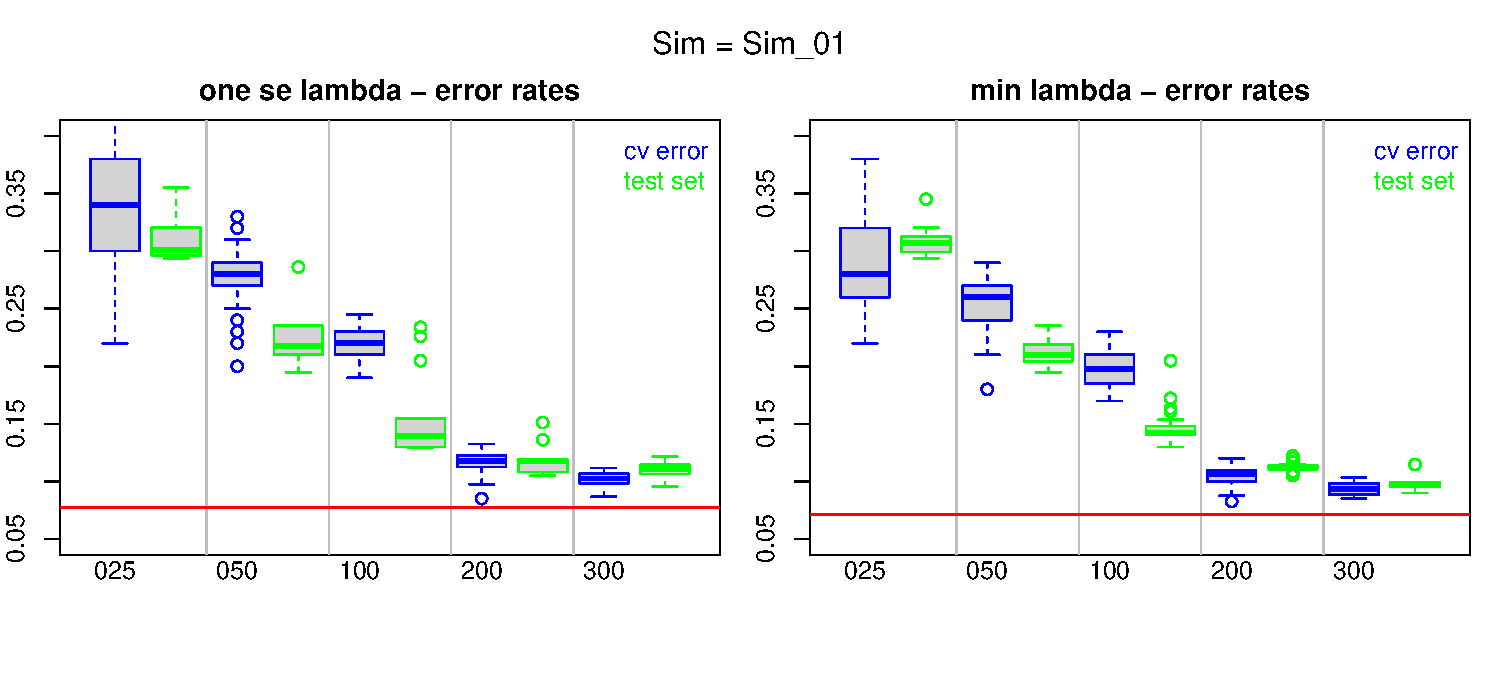
\includegraphics{Static/figures/lasso-simRes-errors-bySim-1.pdf}
\caption{\label{fig:lasso-simRes-errors-bySim}lasso Model Errors by Sample Size}
\end{figure}

In this one simulation, we see:

\begin{itemize}
\item
  Model accuracy increases with sample size, with minimal improvement going from N=200 to N=300.
\item
  CV error rates tend to be pessimistic, expecially for the small sample sizes. This is odd
  and may be related to sample quality.
\item
  There isn't much to chose from between the one standard error and the minimum lambda models. The
  latter may show lower propensity to produce optimistic cv error rates.
\end{itemize}

\begin{Shaded}
\begin{Highlighting}[]
\CommentTok{\#\#\# CLEAR CACHE}

\CommentTok{\# get full model nzero ref}
\NormalTok{nzero\_1se\_vec <{-}}\StringTok{ }\KeywordTok{sapply}\NormalTok{(cv\_lassoAll\_lst,}
 \ControlFlowTok{function}\NormalTok{(cv\_fit) cv\_fit}\OperatorTok{$}\NormalTok{nzero[cv\_fit}\OperatorTok{$}\NormalTok{lambda }\OperatorTok{==}\StringTok{ }\NormalTok{cv\_fit}\OperatorTok{$}\NormalTok{lambda}\FloatTok{.1}\NormalTok{se])}
\NormalTok{nzero\_1se\_q2 <{-}}\StringTok{ }\KeywordTok{quantile}\NormalTok{(nzero\_1se\_vec, }\DataTypeTok{prob=}\KeywordTok{c}\NormalTok{(}\DecValTok{2}\NormalTok{)}\OperatorTok{/}\DecValTok{4}\NormalTok{)}

\NormalTok{nzero\_min\_vec <{-}}\StringTok{ }\KeywordTok{sapply}\NormalTok{(cv\_lassoAll\_lst,}
 \ControlFlowTok{function}\NormalTok{(cv\_fit) cv\_fit}\OperatorTok{$}\NormalTok{nzero[cv\_fit}\OperatorTok{$}\NormalTok{lambda }\OperatorTok{==}\StringTok{ }\NormalTok{cv\_fit}\OperatorTok{$}\NormalTok{lambda.min])}
\NormalTok{nzero\_min\_q2 <{-}}\StringTok{ }\KeywordTok{quantile}\NormalTok{(nzero\_min\_vec, }\DataTypeTok{prob=}\KeywordTok{c}\NormalTok{(}\DecValTok{2}\NormalTok{)}\OperatorTok{/}\DecValTok{4}\NormalTok{)}

\CommentTok{\# Utility objects}
\NormalTok{SIZE0 <{-}}\StringTok{ }\NormalTok{stringr}\OperatorTok{::}\KeywordTok{str\_pad}\NormalTok{(SIZE, }\DataTypeTok{width=}\DecValTok{3}\NormalTok{, }\DataTypeTok{pad=}\StringTok{\textquotesingle{}0\textquotesingle{}}\NormalTok{)}
\NormalTok{stage\_vec <{-}}\StringTok{ }\KeywordTok{cut}\NormalTok{(}\DecValTok{1}\OperatorTok{:}\KeywordTok{nrow}\NormalTok{(sim\_control\_qual\_mtx), }\KeywordTok{c}\NormalTok{(}\DecValTok{0}\NormalTok{,SIZE), }\DataTypeTok{include.lowest =}\NormalTok{ T)}


\CommentTok{\#SIM <{-} "Sim\_01"}

\ControlFlowTok{for}\NormalTok{(SIM }\ControlFlowTok{in} \KeywordTok{unique}\NormalTok{(lasso\_sim\_results\_frm}\OperatorTok{$}\NormalTok{SimNo)[}\DecValTok{1}\NormalTok{])\{}

\NormalTok{SimNum <{-}}\StringTok{ }\KeywordTok{as.numeric}\NormalTok{(}\KeywordTok{sub}\NormalTok{(}\StringTok{\textquotesingle{}Sim\_\textquotesingle{}}\NormalTok{,}\StringTok{\textquotesingle{}\textquotesingle{}}\NormalTok{,SIM))}

\NormalTok{simNo\_results\_frm <{-}}\StringTok{ }\NormalTok{lasso\_sim\_results\_frm }\OperatorTok{\%>\%}\StringTok{ }\NormalTok{dplyr}\OperatorTok{::}\KeywordTok{filter}\NormalTok{(SimNo}\OperatorTok{==}\NormalTok{SIM)}


\KeywordTok{par}\NormalTok{(}\DataTypeTok{mfrow=}\KeywordTok{c}\NormalTok{(}\DecValTok{1}\NormalTok{,}\DecValTok{2}\NormalTok{), }\DataTypeTok{mar=}\KeywordTok{c}\NormalTok{(}\DecValTok{4}\NormalTok{, }\DecValTok{2}\NormalTok{, }\DecValTok{2}\NormalTok{, }\DecValTok{1}\NormalTok{), }\DataTypeTok{oma=}\KeywordTok{c}\NormalTok{(}\DecValTok{0}\NormalTok{,}\DecValTok{0}\NormalTok{,}\DecValTok{2}\NormalTok{,}\DecValTok{0}\NormalTok{))}
\CommentTok{\#\#\#\#\#\#\#\#\#\#\#\#\#\#\#\#\#\#\#}
\CommentTok{\# 1se}
\CommentTok{\#\#\#\#\#\#\#\#\#\#\#\#\#\#\#\#\#\#\#\#}
\CommentTok{\# selected feature counts}
\NormalTok{p\_1se\_lst <{-}}\StringTok{ }\KeywordTok{with}\NormalTok{(simNo\_results\_frm,}
 \KeywordTok{split}\NormalTok{(p\_1se, Size))}
\KeywordTok{names}\NormalTok{(p\_1se\_lst) <{-}}\StringTok{ }\KeywordTok{paste0}\NormalTok{(stringr}\OperatorTok{::}\KeywordTok{str\_pad}\NormalTok{(}\KeywordTok{names}\NormalTok{(p\_1se\_lst), }\DataTypeTok{width=}\DecValTok{3}\NormalTok{, }\DataTypeTok{pad=}\StringTok{\textquotesingle{}0\textquotesingle{}}\NormalTok{),}\StringTok{\textquotesingle{}\_p\textquotesingle{}}\NormalTok{)}

\CommentTok{\# get selected features that are part of lasso\_gene\_sign\_1se\_vec}
\CommentTok{\# {-} the signature selected genes}
\NormalTok{sign\_genes\_1se\_lst <{-}}\StringTok{ }\KeywordTok{lapply}\NormalTok{(}\DecValTok{1}\OperatorTok{:}\KeywordTok{nrow}\NormalTok{(simNo\_results\_frm), }\ControlFlowTok{function}\NormalTok{(RR)}
    \KeywordTok{intersect}\NormalTok{(}\KeywordTok{unlist}\NormalTok{(simNo\_results\_frm[RR, }\StringTok{\textquotesingle{}genes\_1se\textquotesingle{}}\NormalTok{]), lasso\_gene\_sign\_1se\_vec))}

\NormalTok{sign\_p\_1se\_lst <{-}}\StringTok{ }\KeywordTok{split}\NormalTok{(}\KeywordTok{sapply}\NormalTok{(sign\_genes\_1se\_lst, length), simNo\_results\_frm}\OperatorTok{$}\NormalTok{Size)}
\KeywordTok{names}\NormalTok{(sign\_p\_1se\_lst) <{-}}\StringTok{ }\KeywordTok{paste0}\NormalTok{(stringr}\OperatorTok{::}\KeywordTok{str\_pad}\NormalTok{(}\KeywordTok{names}\NormalTok{(sign\_p\_1se\_lst), }\DataTypeTok{width=}\DecValTok{3}\NormalTok{, }\DataTypeTok{pad=}\StringTok{\textquotesingle{}0\textquotesingle{}}\NormalTok{),}\StringTok{\textquotesingle{}\_signP\textquotesingle{}}\NormalTok{)}


\NormalTok{p\_singP\_1se\_lst <{-}}\StringTok{ }\KeywordTok{c}\NormalTok{(p\_1se\_lst, sign\_p\_1se\_lst)}
\NormalTok{p\_singP\_1se\_lst <{-}}\StringTok{ }\NormalTok{p\_singP\_1se\_lst[}\KeywordTok{order}\NormalTok{(}\KeywordTok{names}\NormalTok{(p\_singP\_1se\_lst))]}

\KeywordTok{boxplot}\NormalTok{(p\_singP\_1se\_lst,}
  \DataTypeTok{border=}\KeywordTok{c}\NormalTok{(}\StringTok{\textquotesingle{}blue\textquotesingle{}}\NormalTok{,}\StringTok{\textquotesingle{}green\textquotesingle{}}\NormalTok{),}
  \CommentTok{\#ylim=c(0, 300),}
  \DataTypeTok{xaxt=}\StringTok{\textquotesingle{}n\textquotesingle{}}
\NormalTok{)}
\NormalTok{LL <{-}}\StringTok{ }\DecValTok{{-}1}
\KeywordTok{axis}\NormalTok{(}\DataTypeTok{side=}\DecValTok{1}\NormalTok{, }\DataTypeTok{tick=}\NormalTok{F, }\DataTypeTok{line =}\NormalTok{ LL,}
  \DataTypeTok{at =} \KeywordTok{match}\NormalTok{(}\KeywordTok{paste0}\NormalTok{(SIZE0,}\StringTok{\textquotesingle{}\_p\textquotesingle{}}\NormalTok{),}\KeywordTok{names}\NormalTok{(p\_singP\_1se\_lst)),}
\NormalTok{  SIZE0}
\NormalTok{ )}
\KeywordTok{abline}\NormalTok{(}\DataTypeTok{v=} \KeywordTok{match}\NormalTok{(}\KeywordTok{paste0}\NormalTok{(SIZE0,}\StringTok{\textquotesingle{}\_p\textquotesingle{}}\NormalTok{),}\KeywordTok{names}\NormalTok{(p\_singP\_1se\_lst))[}\OperatorTok{{-}}\DecValTok{1}\NormalTok{] }\OperatorTok{{-}}\StringTok{ }\FloatTok{0.5}\NormalTok{, }\DataTypeTok{col=}\StringTok{\textquotesingle{}grey\textquotesingle{}}\NormalTok{)}
\CommentTok{\#abline(h= nzero\_1se\_q2, col = \textquotesingle{}red\textquotesingle{})}
\KeywordTok{legend}\NormalTok{(}\StringTok{\textquotesingle{}topleft\textquotesingle{}}\NormalTok{,}
   \CommentTok{\#title=\textquotesingle{}1se errors\textquotesingle{}, title.col = \textquotesingle{}black\textquotesingle{},}
   \DataTypeTok{text.col =} \KeywordTok{c}\NormalTok{(}\StringTok{\textquotesingle{}blue\textquotesingle{}}\NormalTok{, }\StringTok{\textquotesingle{}green\textquotesingle{}}\NormalTok{),}
   \DataTypeTok{legend=} \KeywordTok{c}\NormalTok{(}\StringTok{\textquotesingle{}selected genes\textquotesingle{}}\NormalTok{,}\StringTok{\textquotesingle{}signature genes\textquotesingle{}}\NormalTok{),}
   \DataTypeTok{bty=}\StringTok{\textquotesingle{}n\textquotesingle{}}
\NormalTok{ )}
\KeywordTok{title}\NormalTok{(}\KeywordTok{paste}\NormalTok{(}\StringTok{\textquotesingle{}one se lambda {-} selected gene counts\textquotesingle{}}\NormalTok{))}

\NormalTok{SKIP  <{-}}\StringTok{ }\ControlFlowTok{function}\NormalTok{() \{}
\CommentTok{\# Add qual annotation}
\NormalTok{control\_qual\_vec <{-}}\StringTok{ }\KeywordTok{sapply}\NormalTok{(}\KeywordTok{split}\NormalTok{(sim\_control\_qual\_mtx[,SimNum], stage\_vec), median)}
\NormalTok{affected\_qual\_vec <{-}}\StringTok{ }\KeywordTok{sapply}\NormalTok{(}\KeywordTok{split}\NormalTok{(sim\_affected\_qual\_mtx[,SimNum], stage\_vec), median)}
\NormalTok{LL <{-}}\StringTok{ }\NormalTok{LL }\OperatorTok{+}\StringTok{ }\DecValTok{1}
\KeywordTok{axis}\NormalTok{(}\DataTypeTok{side=}\DecValTok{1}\NormalTok{, }\DataTypeTok{tick=}\NormalTok{F, }\DataTypeTok{line =}\NormalTok{ LL,}
  \DataTypeTok{at =}  \KeywordTok{match}\NormalTok{(}\KeywordTok{paste0}\NormalTok{(SIZE0,}\StringTok{\textquotesingle{}\_p\textquotesingle{}}\NormalTok{),}\KeywordTok{names}\NormalTok{(p\_singP\_1se\_lst)),}
  \KeywordTok{round}\NormalTok{(control\_qual\_vec, }\DecValTok{2}\NormalTok{)}
\NormalTok{ )}
\NormalTok{LL <{-}}\StringTok{ }\NormalTok{LL }\OperatorTok{+}\StringTok{ }\DecValTok{1}
\KeywordTok{axis}\NormalTok{(}\DataTypeTok{side=}\DecValTok{1}\NormalTok{, }\DataTypeTok{tick=}\NormalTok{F, }\DataTypeTok{line =}\NormalTok{ LL,}
  \DataTypeTok{at =}  \KeywordTok{match}\NormalTok{(}\KeywordTok{paste0}\NormalTok{(SIZE0,}\StringTok{\textquotesingle{}\_p\textquotesingle{}}\NormalTok{),}\KeywordTok{names}\NormalTok{(p\_singP\_1se\_lst)),}
  \KeywordTok{round}\NormalTok{(affected\_qual\_vec, }\DecValTok{2}\NormalTok{)}
\NormalTok{ )}
\NormalTok{\}}\CommentTok{\#SKIP}

\CommentTok{\#\#\#\#\#\#\#\#\#\#\#\#\#\#\#\#\#\#\#}
\CommentTok{\# min}
\CommentTok{\#\#\#\#\#\#\#\#\#\#\#\#\#\#\#\#\#\#\#\#}
\CommentTok{\# selected feature counts}
\NormalTok{p\_min\_lst <{-}}\StringTok{ }\KeywordTok{with}\NormalTok{(simNo\_results\_frm,}
 \KeywordTok{split}\NormalTok{(p\_min, Size))}
\KeywordTok{names}\NormalTok{(p\_min\_lst) <{-}}\StringTok{ }\KeywordTok{paste0}\NormalTok{(stringr}\OperatorTok{::}\KeywordTok{str\_pad}\NormalTok{(}\KeywordTok{names}\NormalTok{(p\_min\_lst), }\DataTypeTok{width=}\DecValTok{3}\NormalTok{, }\DataTypeTok{pad=}\StringTok{\textquotesingle{}0\textquotesingle{}}\NormalTok{),}\StringTok{\textquotesingle{}\_p\textquotesingle{}}\NormalTok{)}

\CommentTok{\# get selected features that are part of lasso\_gene\_sign\_min\_vec}
\CommentTok{\# {-} the signature selected genes}
\NormalTok{sign\_genes\_min\_lst <{-}}\StringTok{ }\KeywordTok{lapply}\NormalTok{(}\DecValTok{1}\OperatorTok{:}\KeywordTok{nrow}\NormalTok{(simNo\_results\_frm), }\ControlFlowTok{function}\NormalTok{(RR)}
    \KeywordTok{intersect}\NormalTok{(}\KeywordTok{unlist}\NormalTok{(simNo\_results\_frm[RR, }\StringTok{\textquotesingle{}genes\_min\textquotesingle{}}\NormalTok{]), lasso\_gene\_sign\_min\_vec))}

\NormalTok{sign\_p\_min\_lst <{-}}\StringTok{ }\KeywordTok{split}\NormalTok{(}\KeywordTok{sapply}\NormalTok{(sign\_genes\_min\_lst, length), simNo\_results\_frm}\OperatorTok{$}\NormalTok{Size)}
\KeywordTok{names}\NormalTok{(sign\_p\_min\_lst) <{-}}\StringTok{ }\KeywordTok{paste0}\NormalTok{(stringr}\OperatorTok{::}\KeywordTok{str\_pad}\NormalTok{(}\KeywordTok{names}\NormalTok{(sign\_p\_min\_lst), }\DataTypeTok{width=}\DecValTok{3}\NormalTok{, }\DataTypeTok{pad=}\StringTok{\textquotesingle{}0\textquotesingle{}}\NormalTok{),}\StringTok{\textquotesingle{}\_signP\textquotesingle{}}\NormalTok{)}


\NormalTok{p\_singP\_min\_lst <{-}}\StringTok{ }\KeywordTok{c}\NormalTok{(p\_min\_lst, sign\_p\_min\_lst)}
\NormalTok{p\_singP\_min\_lst <{-}}\StringTok{ }\NormalTok{p\_singP\_min\_lst[}\KeywordTok{order}\NormalTok{(}\KeywordTok{names}\NormalTok{(p\_singP\_min\_lst))]}

\KeywordTok{boxplot}\NormalTok{(p\_singP\_min\_lst,}
  \DataTypeTok{border=}\KeywordTok{c}\NormalTok{(}\StringTok{\textquotesingle{}blue\textquotesingle{}}\NormalTok{,}\StringTok{\textquotesingle{}green\textquotesingle{}}\NormalTok{),}
  \CommentTok{\#ylim=c(0, 300),}
  \DataTypeTok{xaxt=}\StringTok{\textquotesingle{}n\textquotesingle{}}
\NormalTok{)}
\NormalTok{LL <{-}}\StringTok{ }\DecValTok{{-}1}
\KeywordTok{axis}\NormalTok{(}\DataTypeTok{side=}\DecValTok{1}\NormalTok{, }\DataTypeTok{tick=}\NormalTok{F, }\DataTypeTok{line =}\NormalTok{ LL,}
  \DataTypeTok{at =} \KeywordTok{match}\NormalTok{(}\KeywordTok{paste0}\NormalTok{(SIZE0,}\StringTok{\textquotesingle{}\_p\textquotesingle{}}\NormalTok{),}\KeywordTok{names}\NormalTok{(p\_singP\_min\_lst)),}
\NormalTok{  SIZE0}
\NormalTok{ )}
\KeywordTok{abline}\NormalTok{(}\DataTypeTok{v=} \KeywordTok{match}\NormalTok{(}\KeywordTok{paste0}\NormalTok{(SIZE0,}\StringTok{\textquotesingle{}\_p\textquotesingle{}}\NormalTok{),}\KeywordTok{names}\NormalTok{(p\_singP\_min\_lst))[}\OperatorTok{{-}}\DecValTok{1}\NormalTok{] }\OperatorTok{{-}}\StringTok{ }\FloatTok{0.5}\NormalTok{, }\DataTypeTok{col=}\StringTok{\textquotesingle{}grey\textquotesingle{}}\NormalTok{)}
\CommentTok{\#abline(h= nzero\_min\_q2, col = \textquotesingle{}red\textquotesingle{})}
\KeywordTok{legend}\NormalTok{(}\StringTok{\textquotesingle{}topleft\textquotesingle{}}\NormalTok{,}
   \CommentTok{\#title=\textquotesingle{}min errors\textquotesingle{}, title.col = \textquotesingle{}black\textquotesingle{},}
   \DataTypeTok{text.col =} \KeywordTok{c}\NormalTok{(}\StringTok{\textquotesingle{}blue\textquotesingle{}}\NormalTok{, }\StringTok{\textquotesingle{}green\textquotesingle{}}\NormalTok{),}
   \DataTypeTok{legend=} \KeywordTok{c}\NormalTok{(}\StringTok{\textquotesingle{}selected genes\textquotesingle{}}\NormalTok{,}\StringTok{\textquotesingle{}signature genes\textquotesingle{}}\NormalTok{),}
   \DataTypeTok{bty=}\StringTok{\textquotesingle{}n\textquotesingle{}}
\NormalTok{ )}
\KeywordTok{title}\NormalTok{(}\KeywordTok{paste}\NormalTok{(}\StringTok{\textquotesingle{}min lambda {-} selected gene counts\textquotesingle{}}\NormalTok{))}

\NormalTok{SKIP  <{-}}\StringTok{ }\ControlFlowTok{function}\NormalTok{() \{}
\CommentTok{\# Add qual annotation}
\NormalTok{control\_qual\_vec <{-}}\StringTok{ }\KeywordTok{sapply}\NormalTok{(}\KeywordTok{split}\NormalTok{(sim\_control\_qual\_mtx[,SimNum], stage\_vec), median)}
\NormalTok{affected\_qual\_vec <{-}}\StringTok{ }\KeywordTok{sapply}\NormalTok{(}\KeywordTok{split}\NormalTok{(sim\_affected\_qual\_mtx[,SimNum], stage\_vec), median)}
\NormalTok{LL <{-}}\StringTok{ }\NormalTok{LL }\OperatorTok{+}\StringTok{ }\DecValTok{1}
\KeywordTok{axis}\NormalTok{(}\DataTypeTok{side=}\DecValTok{1}\NormalTok{, }\DataTypeTok{tick=}\NormalTok{F, }\DataTypeTok{line =}\NormalTok{ LL,}
  \DataTypeTok{at =}  \KeywordTok{match}\NormalTok{(}\KeywordTok{paste0}\NormalTok{(SIZE0,}\StringTok{\textquotesingle{}\_p\textquotesingle{}}\NormalTok{),}\KeywordTok{names}\NormalTok{(p\_singP\_min\_lst)),}
  \KeywordTok{round}\NormalTok{(control\_qual\_vec, }\DecValTok{2}\NormalTok{)}
\NormalTok{ )}
\NormalTok{LL <{-}}\StringTok{ }\NormalTok{LL }\OperatorTok{+}\StringTok{ }\DecValTok{1}
\KeywordTok{axis}\NormalTok{(}\DataTypeTok{side=}\DecValTok{1}\NormalTok{, }\DataTypeTok{tick=}\NormalTok{F, }\DataTypeTok{line =}\NormalTok{ LL,}
  \DataTypeTok{at =}  \KeywordTok{match}\NormalTok{(}\KeywordTok{paste0}\NormalTok{(SIZE0,}\StringTok{\textquotesingle{}\_p\textquotesingle{}}\NormalTok{),}\KeywordTok{names}\NormalTok{(p\_singP\_min\_lst)),}
  \KeywordTok{round}\NormalTok{(affected\_qual\_vec, }\DecValTok{2}\NormalTok{)}
\NormalTok{ )}
\NormalTok{\}}\CommentTok{\#SKIP}

\KeywordTok{mtext}\NormalTok{(}\DataTypeTok{side=}\DecValTok{3}\NormalTok{, }\DataTypeTok{outer=}\NormalTok{T, }\DataTypeTok{cex=}\FloatTok{1.25}\NormalTok{, }\KeywordTok{paste}\NormalTok{(}\StringTok{\textquotesingle{}Sim =\textquotesingle{}}\NormalTok{,  SIM))}

\NormalTok{\} }\CommentTok{\# for(SIM}
\end{Highlighting}
\end{Shaded}

\begin{figure}
\centering
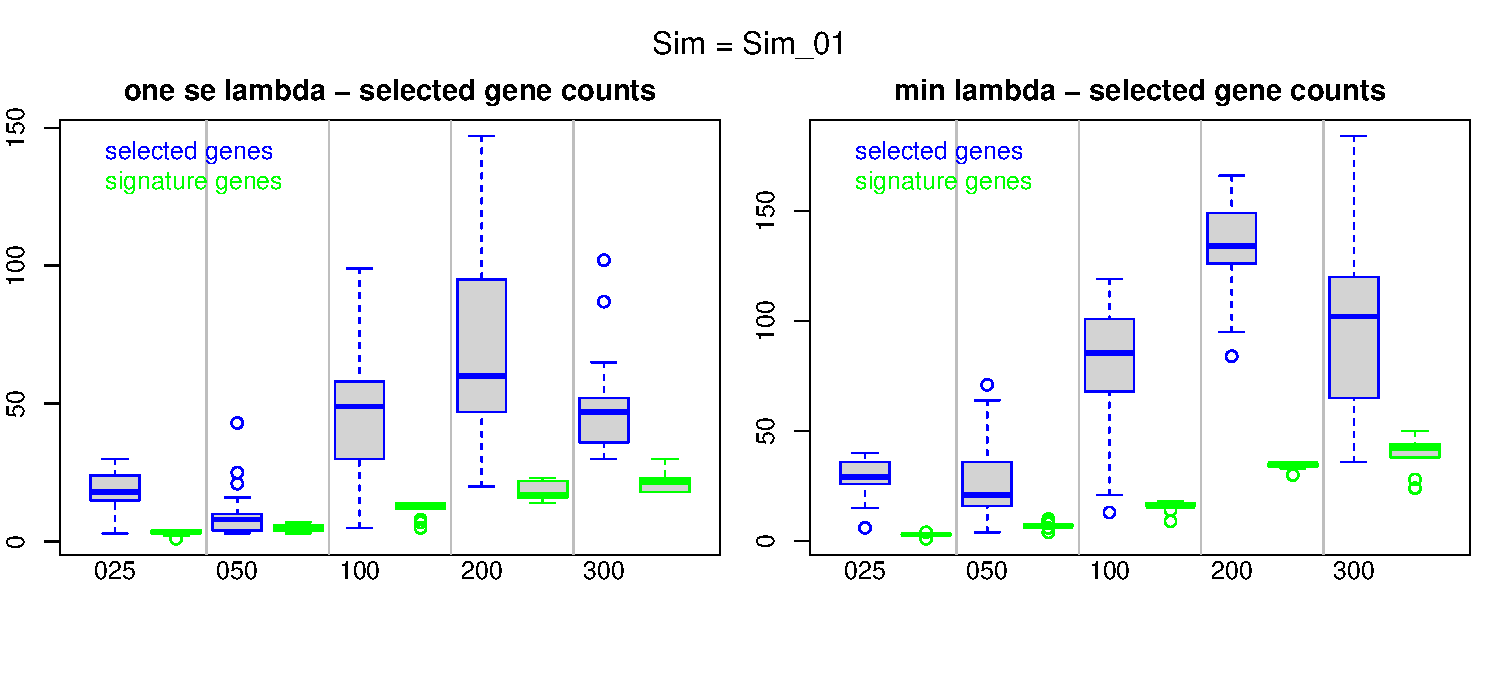
\includegraphics{Static/figures/lasso-simRes-features-bySim-1.pdf}
\caption{\label{fig:lasso-simRes-features-bySim}lasso Models Selected Features by Sample Size}
\end{figure}

In this one simulation, we see:

\begin{itemize}
\item
  The selected number of features in the smaller sample size analyses
  are low, with few feaures belonging to the core signature identified in the
  full data set.
\item
  As the sample size increases the number of features selected in the minimum
  lambda model remains variable, but the number of core signature features
  selected in the samples of sizes 200 and 300 is stable and between 40 and 50.
\end{itemize}

\hypertarget{summarize-results-across-simulation-runs.}{%
\subsection{Summarize results across simulation runs.}\label{summarize-results-across-simulation-runs.}}

Now look acoss all simulations. In the figures that follow, each boxplot
summarizes the results of 30 simulations. For a give sample size and a
given simulation, each data point is the median across 30 repeated cv runs.

\begin{Shaded}
\begin{Highlighting}[]
\CommentTok{\#\#\# CLEAR CACHE}

\CommentTok{\# get full model cv error ref}
\NormalTok{error\_1se\_vec <{-}}\StringTok{ }\KeywordTok{sapply}\NormalTok{(cv\_lassoAll\_lst,}
 \ControlFlowTok{function}\NormalTok{(cv\_fit) cv\_fit}\OperatorTok{$}\NormalTok{cvm[cv\_fit}\OperatorTok{$}\NormalTok{lambda }\OperatorTok{==}\StringTok{ }\NormalTok{cv\_fit}\OperatorTok{$}\NormalTok{lambda}\FloatTok{.1}\NormalTok{se])}
\NormalTok{error\_1se\_q2 <{-}}\StringTok{ }\KeywordTok{quantile}\NormalTok{(error\_1se\_vec, }\DataTypeTok{prob=}\DecValTok{1}\OperatorTok{/}\DecValTok{2}\NormalTok{)        }

\NormalTok{error\_min\_vec <{-}}\StringTok{ }\KeywordTok{sapply}\NormalTok{(cv\_lassoAll\_lst,}
 \ControlFlowTok{function}\NormalTok{(cv\_fit) cv\_fit}\OperatorTok{$}\NormalTok{cvm[cv\_fit}\OperatorTok{$}\NormalTok{lambda }\OperatorTok{==}\StringTok{ }\NormalTok{cv\_fit}\OperatorTok{$}\NormalTok{lambda.min])}
\NormalTok{error\_min\_q2 <{-}}\StringTok{ }\KeywordTok{quantile}\NormalTok{(error\_min\_vec, }\DataTypeTok{prob=}\DecValTok{1}\OperatorTok{/}\DecValTok{2}\NormalTok{)        }

\CommentTok{\# Utility objects}
\NormalTok{SIZE0 <{-}}\StringTok{ }\NormalTok{stringr}\OperatorTok{::}\KeywordTok{str\_pad}\NormalTok{(SIZE, }\DataTypeTok{width=}\DecValTok{3}\NormalTok{, }\DataTypeTok{pad=}\StringTok{\textquotesingle{}0\textquotesingle{}}\NormalTok{)}
\NormalTok{stage\_vec <{-}}\StringTok{ }\KeywordTok{cut}\NormalTok{(}\DecValTok{1}\OperatorTok{:}\KeywordTok{nrow}\NormalTok{(sim\_control\_qual\_mtx), }\KeywordTok{c}\NormalTok{(}\DecValTok{0}\NormalTok{,SIZE), }\DataTypeTok{include.lowest =}\NormalTok{ T)}

\KeywordTok{par}\NormalTok{(}\DataTypeTok{mfrow=}\KeywordTok{c}\NormalTok{(}\DecValTok{1}\NormalTok{,}\DecValTok{2}\NormalTok{), }\DataTypeTok{mar=}\KeywordTok{c}\NormalTok{(}\DecValTok{4}\NormalTok{, }\DecValTok{2}\NormalTok{, }\DecValTok{2}\NormalTok{, }\DecValTok{1}\NormalTok{), }\DataTypeTok{oma=}\KeywordTok{c}\NormalTok{(}\DecValTok{0}\NormalTok{,}\DecValTok{0}\NormalTok{,}\DecValTok{2}\NormalTok{,}\DecValTok{0}\NormalTok{))}
\CommentTok{\# 1se}
\CommentTok{\#\#\#\#\#\#\#\#\#\#\#\#\#\#\#\#\#\#\#\#\#\#\#\#\#\#\#\#\#\#\#\#\#\#\#\#\#\#\#\#\#}
\CommentTok{\#\# cv}
\NormalTok{cv\_1se\_Bysize\_lst <{-}}\StringTok{ }\KeywordTok{lapply}\NormalTok{(}\KeywordTok{unique}\NormalTok{(lasso\_sim\_results\_frm}\OperatorTok{$}\NormalTok{Size),}
\ControlFlowTok{function}\NormalTok{(SizeVal) \{}
\NormalTok{ sizeVal\_results\_frm <{-}}\StringTok{ }\NormalTok{lasso\_sim\_results\_frm }\OperatorTok{\%>\%}\StringTok{ }\NormalTok{dplyr}\OperatorTok{::}\KeywordTok{filter}\NormalTok{(Size}\OperatorTok{==}\NormalTok{SizeVal)}
\NormalTok{ sizeVal\_cv\_1se\_lst <{-}}\StringTok{ }\KeywordTok{with}\NormalTok{(sizeVal\_results\_frm, }\KeywordTok{split}\NormalTok{(cv\_1se, SimNo))}
 \KeywordTok{sapply}\NormalTok{(sizeVal\_cv\_1se\_lst, median)}
\NormalTok{\})}
\KeywordTok{names}\NormalTok{(cv\_1se\_Bysize\_lst) <{-}}\StringTok{ }\KeywordTok{paste0}\NormalTok{(}
\NormalTok{ stringr}\OperatorTok{::}\KeywordTok{str\_pad}\NormalTok{(}\KeywordTok{unique}\NormalTok{(lasso\_sim\_results\_frm}\OperatorTok{$}\NormalTok{Size), }\DataTypeTok{width=}\DecValTok{3}\NormalTok{, }\DataTypeTok{pad=}\StringTok{\textquotesingle{}0\textquotesingle{}}\NormalTok{), }\StringTok{\textquotesingle{}\_cv\textquotesingle{}}\NormalTok{)}

\CommentTok{\#\# test}
\NormalTok{test\_1se\_Bysize\_lst <{-}}\StringTok{ }\KeywordTok{lapply}\NormalTok{(}\KeywordTok{unique}\NormalTok{(lasso\_sim\_results\_frm}\OperatorTok{$}\NormalTok{Size),}
\ControlFlowTok{function}\NormalTok{(SizeVal) \{}
\NormalTok{ sizeVal\_results\_frm <{-}}\StringTok{ }\NormalTok{lasso\_sim\_results\_frm }\OperatorTok{\%>\%}\StringTok{ }\NormalTok{dplyr}\OperatorTok{::}\KeywordTok{filter}\NormalTok{(Size}\OperatorTok{==}\NormalTok{SizeVal)}
\NormalTok{ sizeVal\_test\_1se\_lst <{-}}\StringTok{ }\KeywordTok{with}\NormalTok{(sizeVal\_results\_frm, }\KeywordTok{split}\NormalTok{(test\_1se, SimNo))}
 \KeywordTok{sapply}\NormalTok{(sizeVal\_test\_1se\_lst, median)}
\NormalTok{\})}
\KeywordTok{names}\NormalTok{(test\_1se\_Bysize\_lst) <{-}}\StringTok{ }\KeywordTok{paste0}\NormalTok{(}
\NormalTok{ stringr}\OperatorTok{::}\KeywordTok{str\_pad}\NormalTok{(}\KeywordTok{unique}\NormalTok{(lasso\_sim\_results\_frm}\OperatorTok{$}\NormalTok{Size), }\DataTypeTok{width=}\DecValTok{3}\NormalTok{, }\DataTypeTok{pad=}\StringTok{\textquotesingle{}0\textquotesingle{}}\NormalTok{), }\StringTok{\textquotesingle{}\_test\textquotesingle{}}\NormalTok{)}


\NormalTok{error\_1se\_Bysize\_lst <{-}}\StringTok{ }\KeywordTok{c}\NormalTok{(cv\_1se\_Bysize\_lst, test\_1se\_Bysize\_lst)}
\NormalTok{error\_1se\_Bysize\_lst <{-}}\StringTok{ }\NormalTok{error\_1se\_Bysize\_lst[}\KeywordTok{order}\NormalTok{(}\KeywordTok{names}\NormalTok{(error\_1se\_Bysize\_lst))]}

\KeywordTok{boxplot}\NormalTok{(error\_1se\_Bysize\_lst,}
  \DataTypeTok{col=}\DecValTok{0}\NormalTok{,}
  \DataTypeTok{border=}\KeywordTok{c}\NormalTok{(}\StringTok{\textquotesingle{}blue\textquotesingle{}}\NormalTok{,}\StringTok{\textquotesingle{}green\textquotesingle{}}\NormalTok{),}
  \DataTypeTok{ylim=}\KeywordTok{c}\NormalTok{(}\FloatTok{0.05}\NormalTok{, }\FloatTok{.5}\NormalTok{),}
  \DataTypeTok{outline=}\NormalTok{F,}
  \DataTypeTok{xaxt=}\StringTok{\textquotesingle{}n\textquotesingle{}}
\NormalTok{)}
\ControlFlowTok{for}\NormalTok{(JJ }\ControlFlowTok{in} \DecValTok{1}\OperatorTok{:}\KeywordTok{length}\NormalTok{(error\_1se\_Bysize\_lst))}
\KeywordTok{points}\NormalTok{(}
   \DataTypeTok{x=}\KeywordTok{jitter}\NormalTok{(}\KeywordTok{rep}\NormalTok{(JJ, }\KeywordTok{length}\NormalTok{(error\_1se\_Bysize\_lst[[JJ]])), }\DataTypeTok{amount=}\FloatTok{0.25}\NormalTok{), }
   \DataTypeTok{y=}\NormalTok{error\_1se\_Bysize\_lst[[JJ]],}
   \DataTypeTok{col=}\KeywordTok{ifelse}\NormalTok{(}\KeywordTok{grepl}\NormalTok{(}\StringTok{\textquotesingle{}cv\textquotesingle{}}\NormalTok{, }\KeywordTok{names}\NormalTok{(error\_1se\_Bysize\_lst)[JJ]),}\StringTok{\textquotesingle{}blue\textquotesingle{}}\NormalTok{, }\StringTok{\textquotesingle{}green\textquotesingle{}}\NormalTok{)}
\NormalTok{)}
\NormalTok{LL <{-}}\StringTok{ }\DecValTok{{-}1}
\KeywordTok{axis}\NormalTok{(}\DataTypeTok{side=}\DecValTok{1}\NormalTok{, }\DataTypeTok{tick=}\NormalTok{F, }\DataTypeTok{line =}\NormalTok{ LL,}
  \DataTypeTok{at =} \KeywordTok{match}\NormalTok{(}\KeywordTok{paste0}\NormalTok{(SIZE0,}\StringTok{\textquotesingle{}\_cv\textquotesingle{}}\NormalTok{),}\KeywordTok{names}\NormalTok{(error\_1se\_Bysize\_lst)),}
\NormalTok{  SIZE0}
\NormalTok{ )}
\KeywordTok{abline}\NormalTok{(}\DataTypeTok{v=} \KeywordTok{match}\NormalTok{(}\KeywordTok{paste0}\NormalTok{(SIZE0,}\StringTok{\textquotesingle{}\_cv\textquotesingle{}}\NormalTok{),}\KeywordTok{names}\NormalTok{(error\_1se\_Bysize\_lst))[}\OperatorTok{{-}}\DecValTok{1}\NormalTok{] }\OperatorTok{{-}}\StringTok{ }\FloatTok{0.5}\NormalTok{, }\DataTypeTok{col=}\StringTok{\textquotesingle{}grey\textquotesingle{}}\NormalTok{)}
\KeywordTok{abline}\NormalTok{(}\DataTypeTok{h=}\NormalTok{ error\_min\_q2, }\DataTypeTok{col =} \StringTok{\textquotesingle{}red\textquotesingle{}}\NormalTok{)}
\KeywordTok{legend}\NormalTok{(}\StringTok{\textquotesingle{}topright\textquotesingle{}}\NormalTok{,}
   \CommentTok{\#title=\textquotesingle{}min errors\textquotesingle{}, title.col = \textquotesingle{}black\textquotesingle{},}
   \DataTypeTok{text.col =} \KeywordTok{c}\NormalTok{(}\StringTok{\textquotesingle{}blue\textquotesingle{}}\NormalTok{,}\StringTok{\textquotesingle{}green\textquotesingle{}}\NormalTok{),}
   \DataTypeTok{legend =} \KeywordTok{c}\NormalTok{(}\StringTok{\textquotesingle{}cv error\textquotesingle{}}\NormalTok{, }\StringTok{\textquotesingle{}test set\textquotesingle{}}\NormalTok{),}
   \DataTypeTok{bty=}\StringTok{\textquotesingle{}n\textquotesingle{}}
\NormalTok{ )}
\KeywordTok{title}\NormalTok{(}\KeywordTok{paste}\NormalTok{(}\StringTok{\textquotesingle{}one se lambda {-} error rates\textquotesingle{}}\NormalTok{))}


\CommentTok{\# min}
\CommentTok{\#\#\#\#\#\#\#\#\#\#\#\#\#\#\#\#\#\#\#\#\#\#\#\#\#\#\#\#\#\#\#\#\#\#\#\#\#\#\#\#\#}
\CommentTok{\#\# cv}
\NormalTok{cv\_min\_Bysize\_lst <{-}}\StringTok{ }\KeywordTok{lapply}\NormalTok{(}\KeywordTok{unique}\NormalTok{(lasso\_sim\_results\_frm}\OperatorTok{$}\NormalTok{Size),}
\ControlFlowTok{function}\NormalTok{(SizeVal) \{}
\NormalTok{ sizeVal\_results\_frm <{-}}\StringTok{ }\NormalTok{lasso\_sim\_results\_frm }\OperatorTok{\%>\%}\StringTok{ }\NormalTok{dplyr}\OperatorTok{::}\KeywordTok{filter}\NormalTok{(Size}\OperatorTok{==}\NormalTok{SizeVal)}
\NormalTok{ sizeVal\_cv\_min\_lst <{-}}\StringTok{ }\KeywordTok{with}\NormalTok{(sizeVal\_results\_frm, }\KeywordTok{split}\NormalTok{(cv\_min, SimNo))}
 \KeywordTok{sapply}\NormalTok{(sizeVal\_cv\_min\_lst, median)}
\NormalTok{\})}
\KeywordTok{names}\NormalTok{(cv\_min\_Bysize\_lst) <{-}}\StringTok{ }\KeywordTok{paste0}\NormalTok{(}
\NormalTok{ stringr}\OperatorTok{::}\KeywordTok{str\_pad}\NormalTok{(}\KeywordTok{unique}\NormalTok{(lasso\_sim\_results\_frm}\OperatorTok{$}\NormalTok{Size), }\DataTypeTok{width=}\DecValTok{3}\NormalTok{, }\DataTypeTok{pad=}\StringTok{\textquotesingle{}0\textquotesingle{}}\NormalTok{), }\StringTok{\textquotesingle{}\_cv\textquotesingle{}}\NormalTok{)}

\CommentTok{\#\# test}
\NormalTok{test\_min\_Bysize\_lst <{-}}\StringTok{ }\KeywordTok{lapply}\NormalTok{(}\KeywordTok{unique}\NormalTok{(lasso\_sim\_results\_frm}\OperatorTok{$}\NormalTok{Size),}
\ControlFlowTok{function}\NormalTok{(SizeVal) \{}
\NormalTok{ sizeVal\_results\_frm <{-}}\StringTok{ }\NormalTok{lasso\_sim\_results\_frm }\OperatorTok{\%>\%}\StringTok{ }\NormalTok{dplyr}\OperatorTok{::}\KeywordTok{filter}\NormalTok{(Size}\OperatorTok{==}\NormalTok{SizeVal)}
\NormalTok{ sizeVal\_test\_min\_lst <{-}}\StringTok{ }\KeywordTok{with}\NormalTok{(sizeVal\_results\_frm, }\KeywordTok{split}\NormalTok{(test\_min, SimNo))}
 \KeywordTok{sapply}\NormalTok{(sizeVal\_test\_min\_lst, median)}
\NormalTok{\})}
\KeywordTok{names}\NormalTok{(test\_min\_Bysize\_lst) <{-}}\StringTok{ }\KeywordTok{paste0}\NormalTok{(}
\NormalTok{ stringr}\OperatorTok{::}\KeywordTok{str\_pad}\NormalTok{(}\KeywordTok{unique}\NormalTok{(lasso\_sim\_results\_frm}\OperatorTok{$}\NormalTok{Size), }\DataTypeTok{width=}\DecValTok{3}\NormalTok{, }\DataTypeTok{pad=}\StringTok{\textquotesingle{}0\textquotesingle{}}\NormalTok{), }\StringTok{\textquotesingle{}\_test\textquotesingle{}}\NormalTok{)}


\NormalTok{error\_min\_Bysize\_lst <{-}}\StringTok{ }\KeywordTok{c}\NormalTok{(cv\_min\_Bysize\_lst, test\_min\_Bysize\_lst)}
\NormalTok{error\_min\_Bysize\_lst <{-}}\StringTok{ }\NormalTok{error\_min\_Bysize\_lst[}\KeywordTok{order}\NormalTok{(}\KeywordTok{names}\NormalTok{(error\_min\_Bysize\_lst))]}

\KeywordTok{boxplot}\NormalTok{(error\_min\_Bysize\_lst,}
  \DataTypeTok{col=}\DecValTok{0}\NormalTok{,}
  \DataTypeTok{border=}\KeywordTok{c}\NormalTok{(}\StringTok{\textquotesingle{}blue\textquotesingle{}}\NormalTok{,}\StringTok{\textquotesingle{}green\textquotesingle{}}\NormalTok{),}
  \DataTypeTok{ylim=}\KeywordTok{c}\NormalTok{(}\FloatTok{0.05}\NormalTok{, }\FloatTok{.5}\NormalTok{),}
  \DataTypeTok{outline=}\NormalTok{F,}
  \DataTypeTok{xaxt=}\StringTok{\textquotesingle{}n\textquotesingle{}}
\NormalTok{)}
\ControlFlowTok{for}\NormalTok{(JJ }\ControlFlowTok{in} \DecValTok{1}\OperatorTok{:}\KeywordTok{length}\NormalTok{(error\_min\_Bysize\_lst))}
\KeywordTok{points}\NormalTok{(}
   \DataTypeTok{x=}\KeywordTok{jitter}\NormalTok{(}\KeywordTok{rep}\NormalTok{(JJ, }\KeywordTok{length}\NormalTok{(error\_min\_Bysize\_lst[[JJ]])), }\DataTypeTok{amount=}\FloatTok{0.25}\NormalTok{), }
   \DataTypeTok{y=}\NormalTok{error\_min\_Bysize\_lst[[JJ]],}
   \DataTypeTok{col=}\KeywordTok{ifelse}\NormalTok{(}\KeywordTok{grepl}\NormalTok{(}\StringTok{\textquotesingle{}cv\textquotesingle{}}\NormalTok{, }\KeywordTok{names}\NormalTok{(error\_min\_Bysize\_lst)[JJ]),}\StringTok{\textquotesingle{}blue\textquotesingle{}}\NormalTok{, }\StringTok{\textquotesingle{}green\textquotesingle{}}\NormalTok{)}
\NormalTok{)}
\NormalTok{LL <{-}}\StringTok{ }\DecValTok{{-}1}
\KeywordTok{axis}\NormalTok{(}\DataTypeTok{side=}\DecValTok{1}\NormalTok{, }\DataTypeTok{tick=}\NormalTok{F, }\DataTypeTok{line =}\NormalTok{ LL,}
  \DataTypeTok{at =} \KeywordTok{match}\NormalTok{(}\KeywordTok{paste0}\NormalTok{(SIZE0,}\StringTok{\textquotesingle{}\_cv\textquotesingle{}}\NormalTok{),}\KeywordTok{names}\NormalTok{(error\_min\_Bysize\_lst)),}
\NormalTok{  SIZE0}
\NormalTok{ )}
\KeywordTok{abline}\NormalTok{(}\DataTypeTok{v=} \KeywordTok{match}\NormalTok{(}\KeywordTok{paste0}\NormalTok{(SIZE0,}\StringTok{\textquotesingle{}\_cv\textquotesingle{}}\NormalTok{),}\KeywordTok{names}\NormalTok{(error\_min\_Bysize\_lst))[}\OperatorTok{{-}}\DecValTok{1}\NormalTok{] }\OperatorTok{{-}}\StringTok{ }\FloatTok{0.5}\NormalTok{, }\DataTypeTok{col=}\StringTok{\textquotesingle{}grey\textquotesingle{}}\NormalTok{)}
\KeywordTok{abline}\NormalTok{(}\DataTypeTok{h=}\NormalTok{ error\_min\_q2, }\DataTypeTok{col =} \StringTok{\textquotesingle{}red\textquotesingle{}}\NormalTok{)}
\KeywordTok{legend}\NormalTok{(}\StringTok{\textquotesingle{}topright\textquotesingle{}}\NormalTok{,}
   \CommentTok{\#title=\textquotesingle{}min errors\textquotesingle{}, title.col = \textquotesingle{}black\textquotesingle{},}
   \DataTypeTok{text.col =} \KeywordTok{c}\NormalTok{(}\StringTok{\textquotesingle{}blue\textquotesingle{}}\NormalTok{,}\StringTok{\textquotesingle{}green\textquotesingle{}}\NormalTok{),}
   \DataTypeTok{legend =} \KeywordTok{c}\NormalTok{(}\StringTok{\textquotesingle{}cv error\textquotesingle{}}\NormalTok{, }\StringTok{\textquotesingle{}test set\textquotesingle{}}\NormalTok{),}
   \DataTypeTok{bty=}\StringTok{\textquotesingle{}n\textquotesingle{}}
\NormalTok{ )}
\KeywordTok{title}\NormalTok{(}\KeywordTok{paste}\NormalTok{(}\StringTok{\textquotesingle{}min lambda {-} error rates\textquotesingle{}}\NormalTok{))}


\KeywordTok{mtext}\NormalTok{(}\DataTypeTok{side=}\DecValTok{3}\NormalTok{, }\DataTypeTok{outer=}\NormalTok{T, }\DataTypeTok{cex=}\FloatTok{1.25}\NormalTok{, }\KeywordTok{paste}\NormalTok{(}\StringTok{\textquotesingle{}lasso fit error rates summarized across simulations\textquotesingle{}}\NormalTok{))}
\end{Highlighting}
\end{Shaded}

\begin{figure}
\centering
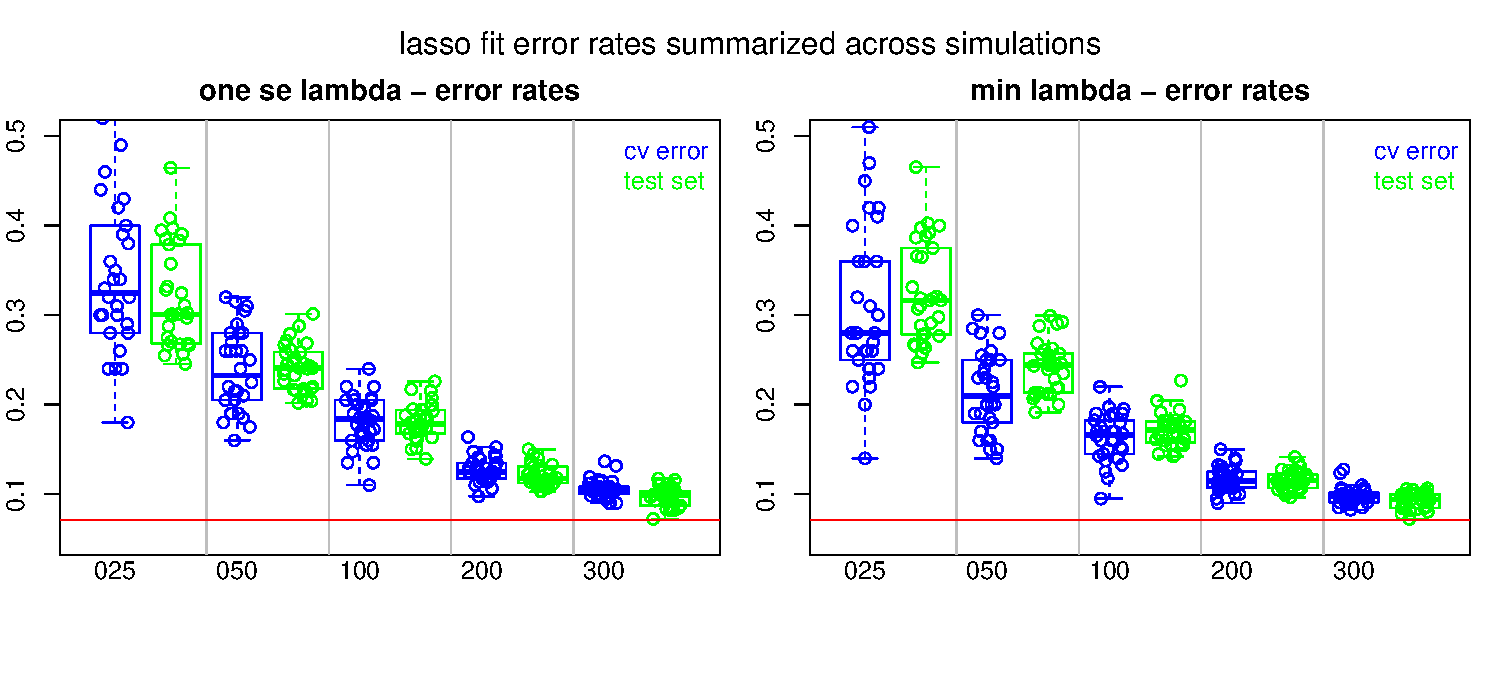
\includegraphics{Static/figures/lasso-simRes-errors-overSim-1.pdf}
\caption{\label{fig:lasso-simRes-errors-overSim}lasso Model Errors by Sample Size}
\end{figure}

\begin{Shaded}
\begin{Highlighting}[]
\CommentTok{\#\#\# CLEAR CACHE}

\NormalTok{error\_1se\_Bysize\_sum\_frm <{-}}\StringTok{ }\KeywordTok{t}\NormalTok{(}\KeywordTok{sapply}\NormalTok{(error\_1se\_Bysize\_lst, }\ControlFlowTok{function}\NormalTok{(LL) }\KeywordTok{quantile}\NormalTok{(LL, }\DataTypeTok{prob=}\NormalTok{(}\DecValTok{1}\OperatorTok{:}\DecValTok{3}\NormalTok{)}\OperatorTok{/}\DecValTok{4}\NormalTok{)))}
\KeywordTok{colnames}\NormalTok{(error\_1se\_Bysize\_sum\_frm) <{-}}\StringTok{ }\KeywordTok{paste0}\NormalTok{(}\StringTok{\textquotesingle{}1se\_\textquotesingle{}}\NormalTok{, }\KeywordTok{colnames}\NormalTok{(error\_1se\_Bysize\_sum\_frm))}

\NormalTok{error\_min\_Bysize\_sum\_frm <{-}}\StringTok{ }\KeywordTok{t}\NormalTok{(}\KeywordTok{sapply}\NormalTok{(error\_min\_Bysize\_lst, }\ControlFlowTok{function}\NormalTok{(LL) }\KeywordTok{quantile}\NormalTok{(LL, }\DataTypeTok{prob=}\NormalTok{(}\DecValTok{1}\OperatorTok{:}\DecValTok{3}\NormalTok{)}\OperatorTok{/}\DecValTok{4}\NormalTok{)))}
\KeywordTok{colnames}\NormalTok{(error\_min\_Bysize\_sum\_frm) <{-}}\StringTok{ }\KeywordTok{paste0}\NormalTok{(}\StringTok{\textquotesingle{}min\_\textquotesingle{}}\NormalTok{, }\KeywordTok{colnames}\NormalTok{(error\_min\_Bysize\_sum\_frm))}


\NormalTok{knitr}\OperatorTok{::}\KeywordTok{kable}\NormalTok{(}\KeywordTok{cbind}\NormalTok{(}\StringTok{\textasciigrave{}}\DataTypeTok{1se}\StringTok{\textasciigrave{}}\NormalTok{=error\_1se\_Bysize\_sum\_frm, }\DataTypeTok{min=}\NormalTok{error\_min\_Bysize\_sum\_frm),}
      \DataTypeTok{caption =} \KeywordTok{paste}\NormalTok{(}\StringTok{"lasso error rates by sample size across simulations"}\NormalTok{),}
    \DataTypeTok{digits=}\DecValTok{2}\NormalTok{) }\OperatorTok{\%>\%}
\StringTok{   }\NormalTok{kableExtra}\OperatorTok{::}\KeywordTok{kable\_styling}\NormalTok{(}\DataTypeTok{full\_width =}\NormalTok{ F)}
\end{Highlighting}
\end{Shaded}

\begin{table}

\caption{\label{tab:print-lasso-simRes-errors-overSim}lasso error rates by sample size across simulations}
\centering
\begin{tabular}[t]{l|r|r|r|r|r|r}
\hline
  & 1se\_25\% & 1se\_50\% & 1se\_75\% & min\_25\% & min\_50\% & min\_75\%\\
\hline
025\_cv & 0.28 & 0.32 & 0.40 & 0.25 & 0.28 & 0.36\\
\hline
025\_test & 0.27 & 0.30 & 0.37 & 0.28 & 0.32 & 0.37\\
\hline
050\_cv & 0.21 & 0.23 & 0.28 & 0.18 & 0.21 & 0.25\\
\hline
050\_test & 0.22 & 0.24 & 0.26 & 0.21 & 0.24 & 0.26\\
\hline
100\_cv & 0.16 & 0.18 & 0.20 & 0.15 & 0.17 & 0.18\\
\hline
100\_test & 0.17 & 0.18 & 0.19 & 0.16 & 0.17 & 0.18\\
\hline
200\_cv & 0.12 & 0.12 & 0.14 & 0.11 & 0.12 & 0.12\\
\hline
200\_test & 0.11 & 0.12 & 0.13 & 0.11 & 0.12 & 0.12\\
\hline
300\_cv & 0.10 & 0.10 & 0.11 & 0.09 & 0.10 & 0.10\\
\hline
300\_test & 0.09 & 0.10 & 0.10 & 0.08 & 0.09 & 0.10\\
\hline
\end{tabular}
\end{table}

\begin{itemize}
\item
  For the smaller samples sizes, cv error rates for the minimum lambda models tend to be
  optimistic.
\item
  For lower sample sizes, assess performance is quite variable.
\end{itemize}

Now look at feature selection.

\begin{Shaded}
\begin{Highlighting}[]
\CommentTok{\#\#\# CLEAR CACHE}

\CommentTok{\# Utility objects}
\NormalTok{SIZE0 <{-}}\StringTok{ }\NormalTok{stringr}\OperatorTok{::}\KeywordTok{str\_pad}\NormalTok{(SIZE, }\DataTypeTok{width=}\DecValTok{3}\NormalTok{, }\DataTypeTok{pad=}\StringTok{\textquotesingle{}0\textquotesingle{}}\NormalTok{)}
\NormalTok{stage\_vec <{-}}\StringTok{ }\KeywordTok{cut}\NormalTok{(}\DecValTok{1}\OperatorTok{:}\KeywordTok{nrow}\NormalTok{(sim\_control\_qual\_mtx), }\KeywordTok{c}\NormalTok{(}\DecValTok{0}\NormalTok{,SIZE), }\DataTypeTok{include.lowest =}\NormalTok{ T)}

\KeywordTok{par}\NormalTok{(}\DataTypeTok{mfrow=}\KeywordTok{c}\NormalTok{(}\DecValTok{1}\NormalTok{,}\DecValTok{2}\NormalTok{), }\DataTypeTok{mar=}\KeywordTok{c}\NormalTok{(}\DecValTok{4}\NormalTok{, }\DecValTok{2}\NormalTok{, }\DecValTok{2}\NormalTok{, }\DecValTok{1}\NormalTok{), }\DataTypeTok{oma=}\KeywordTok{c}\NormalTok{(}\DecValTok{0}\NormalTok{,}\DecValTok{0}\NormalTok{,}\DecValTok{2}\NormalTok{,}\DecValTok{0}\NormalTok{))}
\CommentTok{\# 1se}
\CommentTok{\#\#\#\#\#\#\#\#\#\#\#\#\#\#\#\#\#\#\#\#\#\#\#\#\#\#\#\#\#\#\#\#\#\#\#\#\#\#\#\#\#}
\CommentTok{\# selected features}
\NormalTok{p\_1se\_Bysize\_lst <{-}}\StringTok{ }\KeywordTok{lapply}\NormalTok{(}\KeywordTok{unique}\NormalTok{(lasso\_sim\_results\_frm}\OperatorTok{$}\NormalTok{Size),}
\ControlFlowTok{function}\NormalTok{(SizeVal) \{}
\NormalTok{ sizeVal\_results\_frm <{-}}\StringTok{ }\NormalTok{lasso\_sim\_results\_frm }\OperatorTok{\%>\%}\StringTok{ }\NormalTok{dplyr}\OperatorTok{::}\KeywordTok{filter}\NormalTok{(Size}\OperatorTok{==}\NormalTok{SizeVal)}
\NormalTok{ sizeVal\_p\_1se\_lst <{-}}\StringTok{ }\KeywordTok{with}\NormalTok{(sizeVal\_results\_frm, }\KeywordTok{split}\NormalTok{(p\_1se, SimNo))}
 \KeywordTok{sapply}\NormalTok{(sizeVal\_p\_1se\_lst, median)}
\NormalTok{\})}
\KeywordTok{names}\NormalTok{(p\_1se\_Bysize\_lst) <{-}}\StringTok{ }\KeywordTok{paste0}\NormalTok{(}
\NormalTok{ stringr}\OperatorTok{::}\KeywordTok{str\_pad}\NormalTok{(}\KeywordTok{unique}\NormalTok{(lasso\_sim\_results\_frm}\OperatorTok{$}\NormalTok{Size), }\DataTypeTok{width=}\DecValTok{3}\NormalTok{, }\DataTypeTok{pad=}\StringTok{\textquotesingle{}0\textquotesingle{}}\NormalTok{), }\StringTok{\textquotesingle{}\_p\textquotesingle{}}\NormalTok{)}

\CommentTok{\# selected signatue features}
\NormalTok{sign\_p\_1se\_Bysize\_lst <{-}}\StringTok{ }\KeywordTok{lapply}\NormalTok{(}\KeywordTok{unique}\NormalTok{(lasso\_sim\_results\_frm}\OperatorTok{$}\NormalTok{Size),}
\ControlFlowTok{function}\NormalTok{(SizeVal) \{}
\NormalTok{ sizeVal\_results\_frm <{-}}\StringTok{ }\NormalTok{lasso\_sim\_results\_frm }\OperatorTok{\%>\%}\StringTok{ }\NormalTok{dplyr}\OperatorTok{::}\KeywordTok{filter}\NormalTok{(Size}\OperatorTok{==}\NormalTok{SizeVal)}
 
  
\NormalTok{ sizeVal\_sign\_genes\_1se\_lst <{-}}\StringTok{ }\KeywordTok{lapply}\NormalTok{(}\DecValTok{1}\OperatorTok{:}\KeywordTok{nrow}\NormalTok{(sizeVal\_results\_frm), }\ControlFlowTok{function}\NormalTok{(RR)}
    \KeywordTok{intersect}\NormalTok{(}\KeywordTok{unlist}\NormalTok{(sizeVal\_results\_frm[RR, }\StringTok{\textquotesingle{}genes\_1se\textquotesingle{}}\NormalTok{]), lasso\_gene\_sign\_1se\_vec))}

\NormalTok{ sizeVal\_sign\_p\_1se\_lst <{-}}\StringTok{ }\KeywordTok{split}\NormalTok{(}\KeywordTok{sapply}\NormalTok{(sizeVal\_sign\_genes\_1se\_lst, length),}
\NormalTok{    sizeVal\_results\_frm}\OperatorTok{$}\NormalTok{SimNo)}
 
 \KeywordTok{sapply}\NormalTok{(sizeVal\_sign\_p\_1se\_lst, median)}
\NormalTok{\})}
\KeywordTok{names}\NormalTok{(sign\_p\_1se\_Bysize\_lst) <{-}}\StringTok{ }\KeywordTok{paste0}\NormalTok{(}
\NormalTok{ stringr}\OperatorTok{::}\KeywordTok{str\_pad}\NormalTok{(}\KeywordTok{unique}\NormalTok{(lasso\_sim\_results\_frm}\OperatorTok{$}\NormalTok{Size), }\DataTypeTok{width=}\DecValTok{3}\NormalTok{, }\DataTypeTok{pad=}\StringTok{\textquotesingle{}0\textquotesingle{}}\NormalTok{), }\StringTok{\textquotesingle{}\_signP\textquotesingle{}}\NormalTok{)}


\NormalTok{p\_singP\_1se\_Bysize\_lst <{-}}\StringTok{ }\KeywordTok{c}\NormalTok{(p\_1se\_Bysize\_lst, sign\_p\_1se\_Bysize\_lst)}
\NormalTok{p\_singP\_1se\_Bysize\_lst <{-}}\StringTok{ }\NormalTok{p\_singP\_1se\_Bysize\_lst[}\KeywordTok{order}\NormalTok{(}\KeywordTok{names}\NormalTok{(p\_singP\_1se\_Bysize\_lst))]}

\KeywordTok{boxplot}\NormalTok{(p\_singP\_1se\_Bysize\_lst,}
  \DataTypeTok{col=}\DecValTok{0}\NormalTok{,}
  \DataTypeTok{border=}\KeywordTok{c}\NormalTok{(}\StringTok{\textquotesingle{}blue\textquotesingle{}}\NormalTok{,}\StringTok{\textquotesingle{}green\textquotesingle{}}\NormalTok{),}
  \CommentTok{\#ylim=c(0, 300),}
  \DataTypeTok{xaxt=}\StringTok{\textquotesingle{}n\textquotesingle{}}
\NormalTok{)}
\ControlFlowTok{for}\NormalTok{(JJ }\ControlFlowTok{in} \DecValTok{1}\OperatorTok{:}\KeywordTok{length}\NormalTok{(p\_singP\_1se\_Bysize\_lst))}
\KeywordTok{points}\NormalTok{(}
   \DataTypeTok{x=}\KeywordTok{jitter}\NormalTok{(}\KeywordTok{rep}\NormalTok{(JJ, }\KeywordTok{length}\NormalTok{(p\_singP\_1se\_Bysize\_lst[[JJ]])), }\DataTypeTok{amount=}\FloatTok{0.25}\NormalTok{),}
   \DataTypeTok{y=}\NormalTok{p\_singP\_1se\_Bysize\_lst[[JJ]],}
   \DataTypeTok{col=}\KeywordTok{ifelse}\NormalTok{(}\KeywordTok{grepl}\NormalTok{(}\StringTok{\textquotesingle{}\_p\textquotesingle{}}\NormalTok{, }\KeywordTok{names}\NormalTok{(p\_singP\_1se\_Bysize\_lst)[JJ]),}\StringTok{\textquotesingle{}blue\textquotesingle{}}\NormalTok{, }\StringTok{\textquotesingle{}green\textquotesingle{}}\NormalTok{)}
\NormalTok{)}

\NormalTok{LL <{-}}\StringTok{ }\DecValTok{{-}1}
\KeywordTok{axis}\NormalTok{(}\DataTypeTok{side=}\DecValTok{1}\NormalTok{, }\DataTypeTok{tick=}\NormalTok{F, }\DataTypeTok{line =}\NormalTok{ LL,}
  \DataTypeTok{at =} \KeywordTok{match}\NormalTok{(}\KeywordTok{paste0}\NormalTok{(SIZE0,}\StringTok{\textquotesingle{}\_p\textquotesingle{}}\NormalTok{),}\KeywordTok{names}\NormalTok{(p\_singP\_1se\_Bysize\_lst)),}
\NormalTok{  SIZE0}
\NormalTok{ )}
\KeywordTok{abline}\NormalTok{(}\DataTypeTok{v=} \KeywordTok{match}\NormalTok{(}\KeywordTok{paste0}\NormalTok{(SIZE0,}\StringTok{\textquotesingle{}\_p\textquotesingle{}}\NormalTok{),}\KeywordTok{names}\NormalTok{(p\_singP\_1se\_Bysize\_lst))[}\OperatorTok{{-}}\DecValTok{1}\NormalTok{] }\OperatorTok{{-}}\StringTok{ }\FloatTok{0.5}\NormalTok{, }\DataTypeTok{col=}\StringTok{\textquotesingle{}grey\textquotesingle{}}\NormalTok{)}
\CommentTok{\#abline(h= nzero\_1se\_q2, col = \textquotesingle{}red\textquotesingle{})}
\KeywordTok{legend}\NormalTok{(}\StringTok{\textquotesingle{}topleft\textquotesingle{}}\NormalTok{,}
   \CommentTok{\#title=\textquotesingle{}1se errors\textquotesingle{}, title.col = \textquotesingle{}black\textquotesingle{},}
   \DataTypeTok{text.col =} \KeywordTok{c}\NormalTok{(}\StringTok{\textquotesingle{}blue\textquotesingle{}}\NormalTok{, }\StringTok{\textquotesingle{}green\textquotesingle{}}\NormalTok{),}
   \DataTypeTok{legend=} \KeywordTok{c}\NormalTok{(}\StringTok{\textquotesingle{}selected genes\textquotesingle{}}\NormalTok{,}\StringTok{\textquotesingle{}signature genes\textquotesingle{}}\NormalTok{),}
   \DataTypeTok{bty=}\StringTok{\textquotesingle{}n\textquotesingle{}}
\NormalTok{ )}
\KeywordTok{title}\NormalTok{(}\KeywordTok{paste}\NormalTok{(}\StringTok{\textquotesingle{}one se lamdba {-} selected gene counts\textquotesingle{}}\NormalTok{))}


\CommentTok{\# min}
\CommentTok{\#\#\#\#\#\#\#\#\#\#\#\#\#\#\#\#\#\#\#\#\#\#\#\#\#\#\#\#\#\#\#\#\#\#\#\#\#\#\#\#\#}
\CommentTok{\# selected features}
\NormalTok{p\_min\_Bysize\_lst <{-}}\StringTok{ }\KeywordTok{lapply}\NormalTok{(}\KeywordTok{unique}\NormalTok{(lasso\_sim\_results\_frm}\OperatorTok{$}\NormalTok{Size),}
\ControlFlowTok{function}\NormalTok{(SizeVal) \{}
\NormalTok{ sizeVal\_results\_frm <{-}}\StringTok{ }\NormalTok{lasso\_sim\_results\_frm }\OperatorTok{\%>\%}\StringTok{ }\NormalTok{dplyr}\OperatorTok{::}\KeywordTok{filter}\NormalTok{(Size}\OperatorTok{==}\NormalTok{SizeVal)}
\NormalTok{ sizeVal\_p\_min\_lst <{-}}\StringTok{ }\KeywordTok{with}\NormalTok{(sizeVal\_results\_frm, }\KeywordTok{split}\NormalTok{(p\_min, SimNo))}
 \KeywordTok{sapply}\NormalTok{(sizeVal\_p\_min\_lst, median)}
\NormalTok{\})}
\KeywordTok{names}\NormalTok{(p\_min\_Bysize\_lst) <{-}}\StringTok{ }\KeywordTok{paste0}\NormalTok{(}
\NormalTok{ stringr}\OperatorTok{::}\KeywordTok{str\_pad}\NormalTok{(}\KeywordTok{unique}\NormalTok{(lasso\_sim\_results\_frm}\OperatorTok{$}\NormalTok{Size), }\DataTypeTok{width=}\DecValTok{3}\NormalTok{, }\DataTypeTok{pad=}\StringTok{\textquotesingle{}0\textquotesingle{}}\NormalTok{), }\StringTok{\textquotesingle{}\_p\textquotesingle{}}\NormalTok{)}

\CommentTok{\# selected signatue features}
\NormalTok{sign\_p\_min\_Bysize\_lst <{-}}\StringTok{ }\KeywordTok{lapply}\NormalTok{(}\KeywordTok{unique}\NormalTok{(lasso\_sim\_results\_frm}\OperatorTok{$}\NormalTok{Size),}
\ControlFlowTok{function}\NormalTok{(SizeVal) \{}
\NormalTok{ sizeVal\_results\_frm <{-}}\StringTok{ }\NormalTok{lasso\_sim\_results\_frm }\OperatorTok{\%>\%}\StringTok{ }\NormalTok{dplyr}\OperatorTok{::}\KeywordTok{filter}\NormalTok{(Size}\OperatorTok{==}\NormalTok{SizeVal)}
 
  
\NormalTok{ sizeVal\_sign\_genes\_min\_lst <{-}}\StringTok{ }\KeywordTok{lapply}\NormalTok{(}\DecValTok{1}\OperatorTok{:}\KeywordTok{nrow}\NormalTok{(sizeVal\_results\_frm), }\ControlFlowTok{function}\NormalTok{(RR)}
    \KeywordTok{intersect}\NormalTok{(}\KeywordTok{unlist}\NormalTok{(sizeVal\_results\_frm[RR, }\StringTok{\textquotesingle{}genes\_min\textquotesingle{}}\NormalTok{]), lasso\_gene\_sign\_min\_vec))}

\NormalTok{ sizeVal\_sign\_p\_min\_lst <{-}}\StringTok{ }\KeywordTok{split}\NormalTok{(}\KeywordTok{sapply}\NormalTok{(sizeVal\_sign\_genes\_min\_lst, length),}
\NormalTok{    sizeVal\_results\_frm}\OperatorTok{$}\NormalTok{SimNo)}
 
 \KeywordTok{sapply}\NormalTok{(sizeVal\_sign\_p\_min\_lst, median)}
\NormalTok{\})}
\KeywordTok{names}\NormalTok{(sign\_p\_min\_Bysize\_lst) <{-}}\StringTok{ }\KeywordTok{paste0}\NormalTok{(}
\NormalTok{ stringr}\OperatorTok{::}\KeywordTok{str\_pad}\NormalTok{(}\KeywordTok{unique}\NormalTok{(lasso\_sim\_results\_frm}\OperatorTok{$}\NormalTok{Size), }\DataTypeTok{width=}\DecValTok{3}\NormalTok{, }\DataTypeTok{pad=}\StringTok{\textquotesingle{}0\textquotesingle{}}\NormalTok{), }\StringTok{\textquotesingle{}\_signP\textquotesingle{}}\NormalTok{)}


\NormalTok{p\_singP\_min\_Bysize\_lst <{-}}\StringTok{ }\KeywordTok{c}\NormalTok{(p\_min\_Bysize\_lst, sign\_p\_min\_Bysize\_lst)}
\NormalTok{p\_singP\_min\_Bysize\_lst <{-}}\StringTok{ }\NormalTok{p\_singP\_min\_Bysize\_lst[}\KeywordTok{order}\NormalTok{(}\KeywordTok{names}\NormalTok{(p\_singP\_min\_Bysize\_lst))]}

\KeywordTok{boxplot}\NormalTok{(p\_singP\_min\_Bysize\_lst,}
  \DataTypeTok{col=}\DecValTok{0}\NormalTok{,}
  \DataTypeTok{border=}\KeywordTok{c}\NormalTok{(}\StringTok{\textquotesingle{}blue\textquotesingle{}}\NormalTok{,}\StringTok{\textquotesingle{}green\textquotesingle{}}\NormalTok{),}
  \CommentTok{\#ylim=c(0, 300),}
  \DataTypeTok{xaxt=}\StringTok{\textquotesingle{}n\textquotesingle{}}
\NormalTok{)}
\ControlFlowTok{for}\NormalTok{(JJ }\ControlFlowTok{in} \DecValTok{1}\OperatorTok{:}\KeywordTok{length}\NormalTok{(p\_singP\_min\_Bysize\_lst))}
\KeywordTok{points}\NormalTok{(}
   \DataTypeTok{x=}\KeywordTok{jitter}\NormalTok{(}\KeywordTok{rep}\NormalTok{(JJ, }\KeywordTok{length}\NormalTok{(p\_singP\_min\_Bysize\_lst[[JJ]])), }\DataTypeTok{amount=}\FloatTok{0.25}\NormalTok{),}
   \DataTypeTok{y=}\NormalTok{p\_singP\_min\_Bysize\_lst[[JJ]],}
   \DataTypeTok{col=}\KeywordTok{ifelse}\NormalTok{(}\KeywordTok{grepl}\NormalTok{(}\StringTok{\textquotesingle{}\_p\textquotesingle{}}\NormalTok{, }\KeywordTok{names}\NormalTok{(p\_singP\_min\_Bysize\_lst)[JJ]),}\StringTok{\textquotesingle{}blue\textquotesingle{}}\NormalTok{, }\StringTok{\textquotesingle{}green\textquotesingle{}}\NormalTok{)}
\NormalTok{)}

\NormalTok{LL <{-}}\StringTok{ }\DecValTok{{-}1}
\KeywordTok{axis}\NormalTok{(}\DataTypeTok{side=}\DecValTok{1}\NormalTok{, }\DataTypeTok{tick=}\NormalTok{F, }\DataTypeTok{line =}\NormalTok{ LL,}
  \DataTypeTok{at =} \KeywordTok{match}\NormalTok{(}\KeywordTok{paste0}\NormalTok{(SIZE0,}\StringTok{\textquotesingle{}\_p\textquotesingle{}}\NormalTok{),}\KeywordTok{names}\NormalTok{(p\_singP\_min\_Bysize\_lst)),}
\NormalTok{  SIZE0}
\NormalTok{ )}
\KeywordTok{abline}\NormalTok{(}\DataTypeTok{v=} \KeywordTok{match}\NormalTok{(}\KeywordTok{paste0}\NormalTok{(SIZE0,}\StringTok{\textquotesingle{}\_p\textquotesingle{}}\NormalTok{),}\KeywordTok{names}\NormalTok{(p\_singP\_min\_Bysize\_lst))[}\OperatorTok{{-}}\DecValTok{1}\NormalTok{] }\OperatorTok{{-}}\StringTok{ }\FloatTok{0.5}\NormalTok{, }\DataTypeTok{col=}\StringTok{\textquotesingle{}grey\textquotesingle{}}\NormalTok{)}
\CommentTok{\#abline(h= nzero\_min\_q2, col = \textquotesingle{}red\textquotesingle{})}
\KeywordTok{legend}\NormalTok{(}\StringTok{\textquotesingle{}topleft\textquotesingle{}}\NormalTok{,}
   \CommentTok{\#title=\textquotesingle{}min errors\textquotesingle{}, title.col = \textquotesingle{}black\textquotesingle{},}
   \DataTypeTok{text.col =} \KeywordTok{c}\NormalTok{(}\StringTok{\textquotesingle{}blue\textquotesingle{}}\NormalTok{, }\StringTok{\textquotesingle{}green\textquotesingle{}}\NormalTok{),}
   \DataTypeTok{legend=} \KeywordTok{c}\NormalTok{(}\StringTok{\textquotesingle{}selected genes\textquotesingle{}}\NormalTok{,}\StringTok{\textquotesingle{}signature genes\textquotesingle{}}\NormalTok{),}
   \DataTypeTok{bty=}\StringTok{\textquotesingle{}n\textquotesingle{}}
\NormalTok{ )}
\KeywordTok{title}\NormalTok{(}\KeywordTok{paste}\NormalTok{(}\StringTok{\textquotesingle{}min lambda {-} selected gene counts\textquotesingle{}}\NormalTok{))}

\KeywordTok{mtext}\NormalTok{(}\DataTypeTok{side=}\DecValTok{3}\NormalTok{, }\DataTypeTok{outer=}\NormalTok{T, }\DataTypeTok{cex=}\FloatTok{1.25}\NormalTok{, }\KeywordTok{paste}\NormalTok{(}\StringTok{\textquotesingle{}lasso fit feature selection summarized across simulations\textquotesingle{}}\NormalTok{))}
\end{Highlighting}
\end{Shaded}

\begin{figure}
\centering
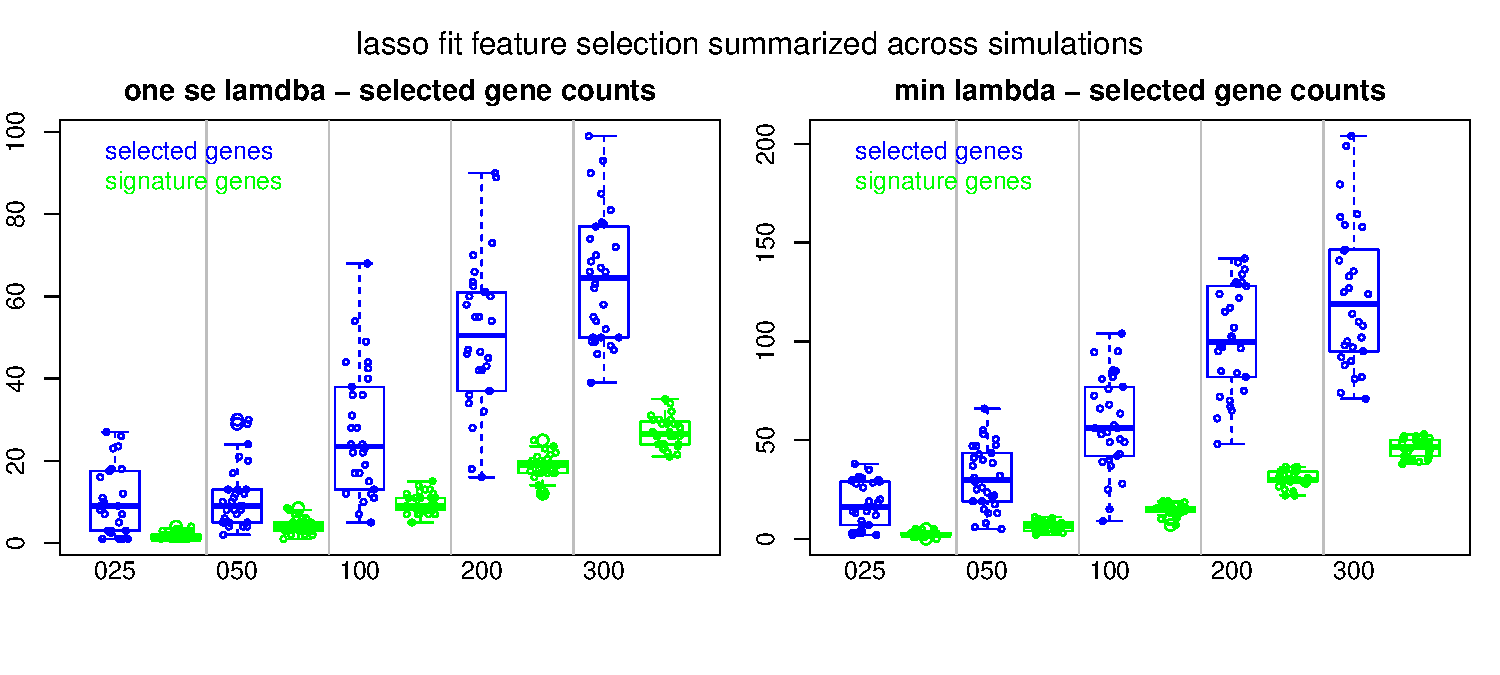
\includegraphics{Static/figures/lasso-simRes-features-OverSim-1.pdf}
\caption{\label{fig:lasso-simRes-features-OverSim}lasso Models Selected Features by Sample Size}
\end{figure}

\begin{Shaded}
\begin{Highlighting}[]
\CommentTok{\#\#\# CLEAR CACHE}

\NormalTok{p\_sing\_1se\_Bysize\_sum\_frm <{-}}\StringTok{ }\KeywordTok{t}\NormalTok{(}\KeywordTok{sapply}\NormalTok{(p\_singP\_1se\_Bysize\_lst, }\ControlFlowTok{function}\NormalTok{(LL) }\KeywordTok{quantile}\NormalTok{(LL, }\DataTypeTok{prob=}\NormalTok{(}\DecValTok{1}\OperatorTok{:}\DecValTok{3}\NormalTok{)}\OperatorTok{/}\DecValTok{4}\NormalTok{)))}
\KeywordTok{colnames}\NormalTok{(p\_sing\_1se\_Bysize\_sum\_frm) <{-}}\StringTok{ }\KeywordTok{paste0}\NormalTok{(}\StringTok{\textquotesingle{}1se\_\textquotesingle{}}\NormalTok{, }\KeywordTok{colnames}\NormalTok{(p\_sing\_1se\_Bysize\_sum\_frm))}
 
\NormalTok{p\_sing\_min\_Bysize\_sum\_frm <{-}}\StringTok{ }\KeywordTok{t}\NormalTok{(}\KeywordTok{sapply}\NormalTok{(p\_singP\_min\_Bysize\_lst, }\ControlFlowTok{function}\NormalTok{(LL) }\KeywordTok{quantile}\NormalTok{(LL, }\DataTypeTok{prob=}\NormalTok{(}\DecValTok{1}\OperatorTok{:}\DecValTok{3}\NormalTok{)}\OperatorTok{/}\DecValTok{4}\NormalTok{)))}
\KeywordTok{colnames}\NormalTok{(p\_sing\_min\_Bysize\_sum\_frm) <{-}}\StringTok{ }\KeywordTok{paste0}\NormalTok{(}\StringTok{\textquotesingle{}min\_\textquotesingle{}}\NormalTok{, }\KeywordTok{colnames}\NormalTok{(p\_sing\_min\_Bysize\_sum\_frm))}

\NormalTok{knitr}\OperatorTok{::}\KeywordTok{kable}\NormalTok{(}\KeywordTok{cbind}\NormalTok{(p\_sing\_1se\_Bysize\_sum\_frm, p\_sing\_min\_Bysize\_sum\_frm),}
    \DataTypeTok{caption =} \KeywordTok{paste}\NormalTok{(}\StringTok{"lasso feature selection by sample size across simulations"}\NormalTok{),}
    \DataTypeTok{digits=}\DecValTok{2}\NormalTok{) }\OperatorTok{\%>\%}
\StringTok{   }\NormalTok{kableExtra}\OperatorTok{::}\KeywordTok{kable\_styling}\NormalTok{(}\DataTypeTok{full\_width =}\NormalTok{ F)}
\end{Highlighting}
\end{Shaded}

\begin{table}

\caption{\label{tab:print-lasso-simRes-features-OverSim}lasso feature selection by sample size across simulations}
\centering
\begin{tabular}[t]{l|r|r|r|r|r|r}
\hline
  & 1se\_25\% & 1se\_50\% & 1se\_75\% & min\_25\% & min\_50\% & min\_75\%\\
\hline
025\_p & 3.00 & 9.0 & 17.50 & 7.00 & 16.00 & 28.88\\
\hline
025\_signP & 1.00 & 1.0 & 2.00 & 2.00 & 2.00 & 3.00\\
\hline
050\_p & 5.00 & 9.0 & 13.00 & 19.00 & 30.00 & 43.38\\
\hline
050\_signP & 3.00 & 4.0 & 5.00 & 4.50 & 6.50 & 8.38\\
\hline
100\_p & 13.50 & 23.5 & 37.50 & 42.25 & 56.00 & 76.75\\
\hline
100\_signP & 8.00 & 9.0 & 11.00 & 14.00 & 15.00 & 16.00\\
\hline
200\_p & 38.25 & 50.5 & 61.00 & 82.50 & 99.75 & 127.00\\
\hline
200\_signP & 17.00 & 19.0 & 20.00 & 29.00 & 30.00 & 33.75\\
\hline
300\_p & 50.00 & 64.5 & 76.25 & 95.50 & 119.00 & 146.38\\
\hline
300\_signP & 24.00 & 26.5 & 29.38 & 42.25 & 46.50 & 49.75\\
\hline
\end{tabular}
\end{table}

\begin{itemize}
\item
  The number of selected features incerase with sample size.
\item
  The number of selected features is quite variable, even for larger sample sizes.
\item
  The number of core signature features among selected features is stable for larger sample
  sizes and represenst 30 to 40\% of the selected features (for N=200 and 300 respectively).
\end{itemize}

\hypertarget{effect-of-sample-quality}{%
\section{Effect of sample quality}\label{effect-of-sample-quality}}

To see the effect of sample quality on classification results, we will
focus on the performance of the small sample fits where variability is the
greatest, and the context where investigators should be most aware of the
effect of sample selection over and beyond sample size concerns.

\begin{Shaded}
\begin{Highlighting}[]
\NormalTok{control\_samp25\_qual\_vec <{-}}\StringTok{ }\KeywordTok{apply}\NormalTok{(sim\_control\_qual\_mtx[}\DecValTok{1}\OperatorTok{:}\DecValTok{25}\NormalTok{, ], }\DecValTok{2}\NormalTok{, median)}
\NormalTok{affected\_samp25\_qual\_vec <{-}}\StringTok{ }\KeywordTok{apply}\NormalTok{(sim\_affected\_qual\_mtx[}\DecValTok{1}\OperatorTok{:}\DecValTok{25}\NormalTok{, ], }\DecValTok{2}\NormalTok{, median)}

\NormalTok{samp25\_qual\_error\_mtx <{-}}\StringTok{ }\KeywordTok{cbind}\NormalTok{(}
   \StringTok{\textasciigrave{}}\DataTypeTok{1se\_cv}\StringTok{\textasciigrave{}}\NormalTok{ =}\StringTok{ }\NormalTok{error\_1se\_Bysize\_lst[[}\StringTok{\textquotesingle{}025\_cv\textquotesingle{}}\NormalTok{]],}
   \StringTok{\textasciigrave{}}\DataTypeTok{1se\_test}\StringTok{\textasciigrave{}}\NormalTok{ =}\StringTok{ }\NormalTok{error\_1se\_Bysize\_lst[[}\StringTok{\textquotesingle{}025\_test\textquotesingle{}}\NormalTok{]],}
   \StringTok{\textasciigrave{}}\DataTypeTok{control\_Q}\StringTok{\textasciigrave{}}\NormalTok{ =}\StringTok{ }\NormalTok{control\_samp25\_qual\_vec,}
   \StringTok{\textasciigrave{}}\DataTypeTok{affected\_Q}\StringTok{\textasciigrave{}}\NormalTok{ =}\StringTok{ }\NormalTok{affected\_samp25\_qual\_vec)}
 

\CommentTok{\# Correlation panel}
\NormalTok{panel.cor <{-}}\StringTok{ }\ControlFlowTok{function}\NormalTok{(x, y)\{}
\NormalTok{    usr <{-}}\StringTok{ }\KeywordTok{par}\NormalTok{(}\StringTok{"usr"}\NormalTok{); }\KeywordTok{on.exit}\NormalTok{(}\KeywordTok{par}\NormalTok{(usr))}
    \KeywordTok{par}\NormalTok{(}\DataTypeTok{usr =} \KeywordTok{c}\NormalTok{(}\DecValTok{0}\NormalTok{, }\DecValTok{1}\NormalTok{, }\DecValTok{0}\NormalTok{, }\DecValTok{1}\NormalTok{))}
\NormalTok{    r <{-}}\StringTok{ }\KeywordTok{round}\NormalTok{(}\KeywordTok{cor}\NormalTok{(x, y), }\DataTypeTok{digits=}\DecValTok{2}\NormalTok{)}
\NormalTok{    txt <{-}}\StringTok{ }\KeywordTok{paste0}\NormalTok{(}\StringTok{"R = "}\NormalTok{, r)}
\NormalTok{    cex.cor <{-}}\StringTok{ }\FloatTok{0.8}\OperatorTok{/}\KeywordTok{strwidth}\NormalTok{(txt)}
    \KeywordTok{text}\NormalTok{(}\FloatTok{0.5}\NormalTok{, }\FloatTok{0.5}\NormalTok{, txt, }\DataTypeTok{cex =} \FloatTok{1.5}\NormalTok{) }\CommentTok{\#\#\#cex.cor * r)}
\NormalTok{\}}

\KeywordTok{pairs}\NormalTok{(samp25\_qual\_error\_mtx,}
 \DataTypeTok{lower.panel =}\NormalTok{ panel.cor)}
\end{Highlighting}
\end{Shaded}

\begin{figure}
\centering
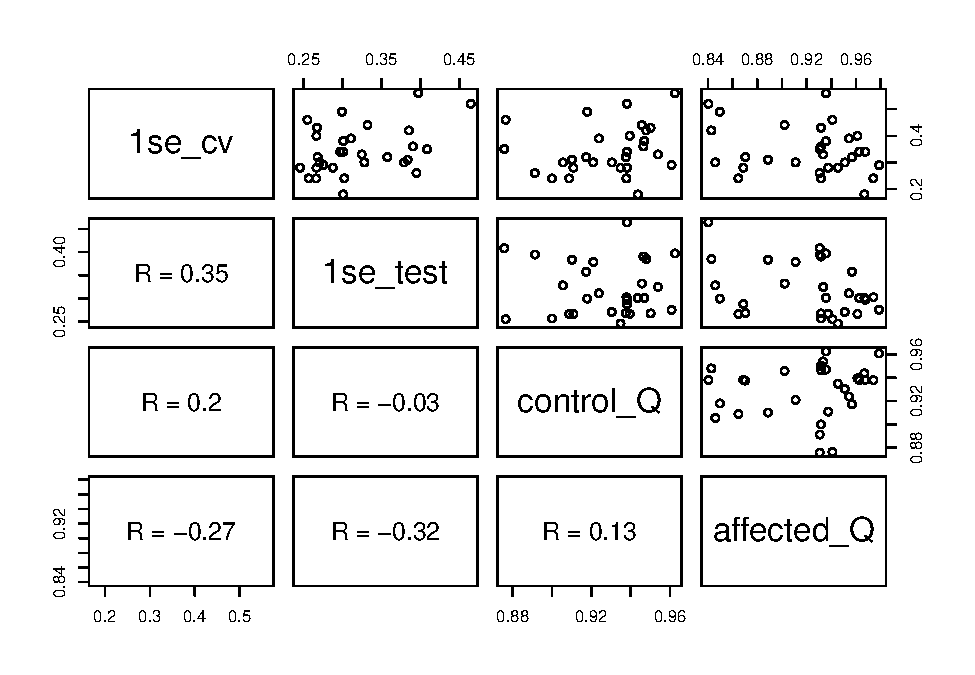
\includegraphics{Static/figures/small-sample-qual-1.pdf}
\caption{\label{fig:small-sample-qual}sample quality vs classifier performance}
\end{figure}

We see that although the sample quality effect is not strong, the quality of the
affected sample cohorts does have a measurable impact on the 1se cv and test set error
rates (cor = -0.32 and -0.27, respectively).

\hypertarget{conclusions}{%
\chapter{Conclusions}\label{conclusions}}

We have found that \ldots{}

Other questions \ldots{}

\hypertarget{appendix-1}{%
\chapter*{Appendix 1 - Sample size in elastic net fits}\label{appendix-1}}
\addcontentsline{toc}{chapter}{Appendix 1 - Sample size in elastic net fits}

Repeat the analyses from Section \ref{model-suite}, but using
the elastic net as classfication model.

\begin{Shaded}
\begin{Highlighting}[]
\KeywordTok{set.seed}\NormalTok{(}\DecValTok{1}\NormalTok{)}

\NormalTok{start\_time <{-}}\StringTok{  }\KeywordTok{proc.time}\NormalTok{()}

\NormalTok{cv\_enetAll\_lst <{-}}\StringTok{ }\KeywordTok{lapply}\NormalTok{(}\DecValTok{1}\OperatorTok{:}\DecValTok{30}\NormalTok{, }\ControlFlowTok{function}\NormalTok{(REP) \{}
\NormalTok{glmnet}\OperatorTok{::}\KeywordTok{cv.glmnet}\NormalTok{(}
 \DataTypeTok{x =}\NormalTok{ all\_lcpm\_mtx,}
 \DataTypeTok{y =} \KeywordTok{factor}\NormalTok{(all\_group\_vec,}\DataTypeTok{levels =} \KeywordTok{c}\NormalTok{(}\StringTok{\textquotesingle{}Control\textquotesingle{}}\NormalTok{, }\StringTok{\textquotesingle{}HCC\textquotesingle{}}\NormalTok{)),}
 \DataTypeTok{alpha =} \FloatTok{0.5}\NormalTok{,}
 \DataTypeTok{family =} \StringTok{\textquotesingle{}binomial\textquotesingle{}}\NormalTok{,}
 \DataTypeTok{type.measure  =}  \StringTok{"class"}\NormalTok{,}
 \DataTypeTok{keep =}\NormalTok{ T,}
 \DataTypeTok{nlambda =} \DecValTok{100}
\NormalTok{)}
\NormalTok{\}}
\NormalTok{)}

\KeywordTok{message}\NormalTok{(}\StringTok{"enetAll time: "}\NormalTok{, }\KeywordTok{round}\NormalTok{((}\KeywordTok{proc.time}\NormalTok{() }\OperatorTok{{-}}\StringTok{ }\NormalTok{start\_time)[}\DecValTok{3}\NormalTok{],}\DecValTok{2}\NormalTok{),}\StringTok{"s"}\NormalTok{)}
\end{Highlighting}
\end{Shaded}

Examine the fits.

\begin{Shaded}
\begin{Highlighting}[]
\CommentTok{\#\#\# CLEAR CACHE}
\KeywordTok{plot}\NormalTok{(}
 \KeywordTok{log}\NormalTok{(cv\_enetAll\_lst[[}\DecValTok{1}\NormalTok{]]}\OperatorTok{$}\NormalTok{lambda),}
\NormalTok{ cv\_enetAll\_lst[[}\DecValTok{1}\NormalTok{]]}\OperatorTok{$}\NormalTok{cvm,}
 \DataTypeTok{lwd=}\DecValTok{2}\NormalTok{,}
 \DataTypeTok{xlab=}\StringTok{\textquotesingle{}log(Lambda)\textquotesingle{}}\NormalTok{, }\DataTypeTok{ylab=}\StringTok{\textquotesingle{}CV Misclassification Error\textquotesingle{}}\NormalTok{, }\DataTypeTok{type=}\StringTok{\textquotesingle{}l\textquotesingle{}}\NormalTok{, }\DataTypeTok{ylim=}\KeywordTok{c}\NormalTok{(}\DecValTok{0}\NormalTok{, }\FloatTok{.5}\NormalTok{)}
\NormalTok{)}

\ControlFlowTok{for}\NormalTok{(JJ }\ControlFlowTok{in} \DecValTok{2}\OperatorTok{:}\KeywordTok{length}\NormalTok{(cv\_enetAll\_lst))}
 \KeywordTok{lines}\NormalTok{(}
  \KeywordTok{log}\NormalTok{(cv\_enetAll\_lst[[JJ]]}\OperatorTok{$}\NormalTok{lambda),}
\NormalTok{  cv\_enetAll\_lst[[JJ]]}\OperatorTok{$}\NormalTok{cvm,}
  \DataTypeTok{lwd=}\DecValTok{2}
\NormalTok{)}
\end{Highlighting}
\end{Shaded}

\begin{figure}
\centering
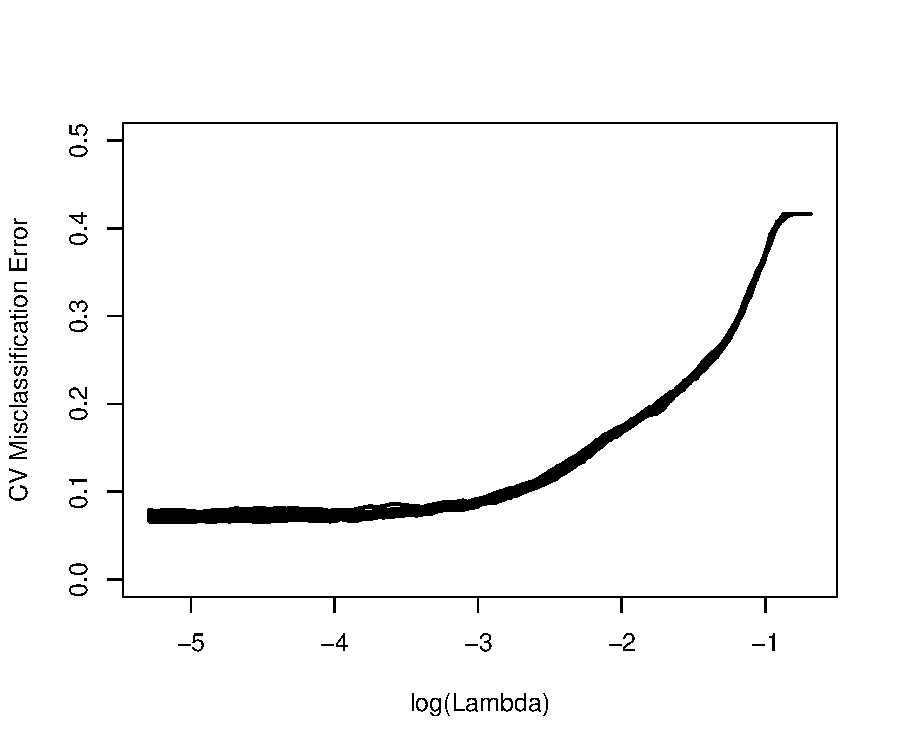
\includegraphics{Static/figures/enet-plot-enetAll-1.pdf}
\caption{\label{fig:enet-plot-enetAll}Repeated cv enet models fitted to all samples}
\end{figure}

These cv curves are again remarkably consistent meaning that the determination of the size or sparsity
of the model through cross validation is fairly precise:

\begin{Shaded}
\begin{Highlighting}[]
\KeywordTok{library}\NormalTok{(magrittr)}

\KeywordTok{par}\NormalTok{(}\DataTypeTok{mfrow=}\KeywordTok{c}\NormalTok{(}\DecValTok{1}\NormalTok{,}\DecValTok{2}\NormalTok{), }\DataTypeTok{mar=}\KeywordTok{c}\NormalTok{(}\DecValTok{3}\NormalTok{,}\DecValTok{4}\NormalTok{, }\DecValTok{2}\NormalTok{, }\DecValTok{1}\NormalTok{))}

\CommentTok{\# nzero}
\NormalTok{nzero\_1se\_vec <{-}}\StringTok{ }\KeywordTok{sapply}\NormalTok{(cv\_enetAll\_lst,}
 \ControlFlowTok{function}\NormalTok{(cv\_fit) cv\_fit}\OperatorTok{$}\NormalTok{nzero[cv\_fit}\OperatorTok{$}\NormalTok{lambda }\OperatorTok{==}\StringTok{ }\NormalTok{cv\_fit}\OperatorTok{$}\NormalTok{lambda}\FloatTok{.1}\NormalTok{se])}

\NormalTok{nzero\_min\_vec <{-}}\StringTok{ }\KeywordTok{sapply}\NormalTok{(cv\_enetAll\_lst,}
 \ControlFlowTok{function}\NormalTok{(cv\_fit) cv\_fit}\OperatorTok{$}\NormalTok{nzero[cv\_fit}\OperatorTok{$}\NormalTok{lambda }\OperatorTok{==}\StringTok{ }\NormalTok{cv\_fit}\OperatorTok{$}\NormalTok{lambda.min])}

\KeywordTok{boxplot}\NormalTok{(}\KeywordTok{list}\NormalTok{(}\StringTok{\textasciigrave{}}\DataTypeTok{1se}\StringTok{\textasciigrave{}}\NormalTok{=nzero\_1se\_vec, }\DataTypeTok{min =}\NormalTok{ nzero\_min\_vec), }\DataTypeTok{ylab=}\StringTok{"Full Model cv Summary"}\NormalTok{)}

\CommentTok{\# error}
\NormalTok{error\_1se\_vec <{-}}\StringTok{ }\KeywordTok{sapply}\NormalTok{(cv\_enetAll\_lst,}
 \ControlFlowTok{function}\NormalTok{(cv\_fit) cv\_fit}\OperatorTok{$}\NormalTok{cvm[cv\_fit}\OperatorTok{$}\NormalTok{lambda }\OperatorTok{==}\StringTok{ }\NormalTok{cv\_fit}\OperatorTok{$}\NormalTok{lambda}\FloatTok{.1}\NormalTok{se])}

\NormalTok{error\_min\_vec <{-}}\StringTok{ }\KeywordTok{sapply}\NormalTok{(cv\_enetAll\_lst,}
 \ControlFlowTok{function}\NormalTok{(cv\_fit) cv\_fit}\OperatorTok{$}\NormalTok{cvm[cv\_fit}\OperatorTok{$}\NormalTok{lambda }\OperatorTok{==}\StringTok{ }\NormalTok{cv\_fit}\OperatorTok{$}\NormalTok{lambda.min])}

\KeywordTok{boxplot}\NormalTok{(}
 \KeywordTok{list}\NormalTok{(}\StringTok{\textasciigrave{}}\DataTypeTok{1se}\StringTok{\textasciigrave{}}\NormalTok{=error\_1se\_vec, }\DataTypeTok{min =}\NormalTok{ error\_min\_vec), }
 \DataTypeTok{ylab=}\NormalTok{cv\_enetAll\_lst[[}\DecValTok{1}\NormalTok{]]}\OperatorTok{$}\NormalTok{name,}
 \DataTypeTok{ylim=}\KeywordTok{c}\NormalTok{(}\FloatTok{0.06}\NormalTok{, }\FloatTok{.10}\NormalTok{)}
\NormalTok{)}
\end{Highlighting}
\end{Shaded}

\begin{figure}
\centering
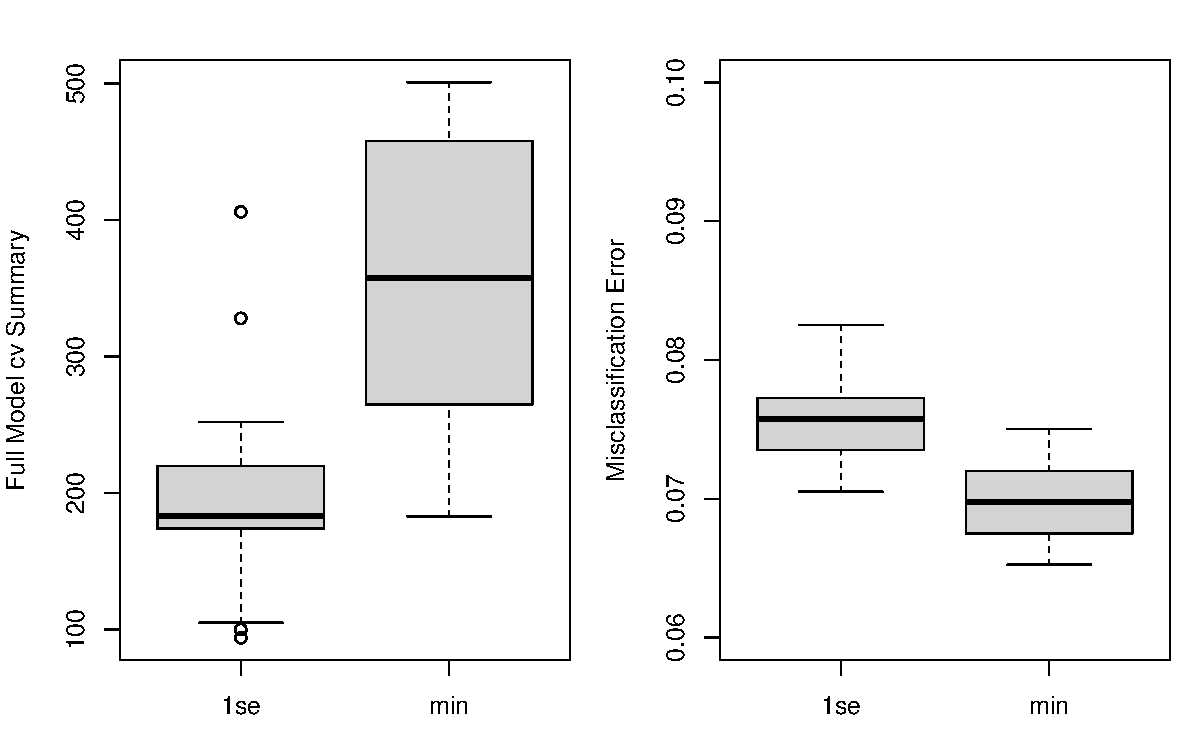
\includegraphics{Static/figures/model-size-enetAll-1.pdf}
\caption{\label{fig:model-size-enetAll}Feature selection and estimated error by repeated cv enet models}
\end{figure}

\begin{Shaded}
\begin{Highlighting}[]
\CommentTok{\# tabular format}
\NormalTok{tmp <{-}}\StringTok{ }\KeywordTok{data.frame}\NormalTok{(}\KeywordTok{rbind}\NormalTok{(}
 \StringTok{\textasciigrave{}}\DataTypeTok{features\_1se}\StringTok{\textasciigrave{}}\NormalTok{ =}\StringTok{ }\KeywordTok{summary}\NormalTok{(nzero\_1se\_vec),}
 \DataTypeTok{features\_min =} \KeywordTok{summary}\NormalTok{(nzero\_min\_vec),}
 \StringTok{\textasciigrave{}}\DataTypeTok{features:min{-}1se}\StringTok{\textasciigrave{}}\NormalTok{ =}\StringTok{ }\KeywordTok{summary}\NormalTok{(nzero\_min\_vec }\OperatorTok{{-}}\StringTok{ }\NormalTok{nzero\_1se\_vec),}
 \StringTok{\textasciigrave{}}\DataTypeTok{cv\_error\_1se}\StringTok{\textasciigrave{}}\NormalTok{ =}\StringTok{ }\KeywordTok{summary}\NormalTok{(}\DecValTok{100}\OperatorTok{*}\NormalTok{error\_1se\_vec),}
 \DataTypeTok{cv\_error\_min =} \KeywordTok{summary}\NormalTok{(}\DecValTok{100}\OperatorTok{*}\NormalTok{error\_min\_vec),}
 \StringTok{\textasciigrave{}}\DataTypeTok{cv\_error:1se{-}min}\StringTok{\textasciigrave{}}\NormalTok{ =}\StringTok{ }\KeywordTok{summary}\NormalTok{(}\DecValTok{100}\OperatorTok{*}\NormalTok{(error\_1se\_vec}\OperatorTok{{-}}\NormalTok{error\_min\_vec))}
\NormalTok{))}

\NormalTok{knitr}\OperatorTok{::}\KeywordTok{kable}\NormalTok{(tmp }\OperatorTok{\%>\%}\StringTok{ }\NormalTok{dplyr}\OperatorTok{::}\KeywordTok{select}\NormalTok{(}\OperatorTok{{-}}\NormalTok{Mean),}
  \DataTypeTok{caption =} \StringTok{"Number of selected features"}\NormalTok{,}
  \DataTypeTok{digits=}\DecValTok{1}\NormalTok{) }\OperatorTok{\%>\%}
\StringTok{   }\NormalTok{kableExtra}\OperatorTok{::}\KeywordTok{kable\_styling}\NormalTok{(}\DataTypeTok{full\_width =}\NormalTok{ F)}
\end{Highlighting}
\end{Shaded}

\begin{table}

\caption{\label{tab:model-size-enetAll}Number of selected features}
\centering
\begin{tabular}[t]{l|r|r|r|r|r}
\hline
  & Min. & X1st.Qu. & Median & X3rd.Qu. & Max.\\
\hline
features\_1se & 94.0 & 174.0 & 183.0 & 215.0 & 406.0\\
\hline
features\_min & 183.0 & 271.5 & 357.5 & 457.2 & 501.0\\
\hline
features:min-1se & 23.0 & 81.5 & 168.5 & 237.5 & 331.0\\
\hline
cv\_error\_1se & 7.1 & 7.4 & 7.6 & 7.7 & 8.3\\
\hline
cv\_error\_min & 6.5 & 6.8 & 7.0 & 7.2 & 7.5\\
\hline
cv\_error:1se-min & 0.2 & 0.5 & 0.6 & 0.7 & 0.9\\
\hline
\end{tabular}
\end{table}

The number of features selected by the minimum lambda model is larger
than the number selected by the ``one standard error'' rule by a median
of \(168.5\) and results on
a median reduction in cv error rates of
\(0.6\)\%.

The cv error rates observed in this set are comparable to the
rates oberved in the enet models fitted to the training sample set
which consisted of 80\% of the samples in this set. See Table \ref{tab:printErrors}.
It's not clear at this point whether the minimum lambda model is better than
the ``one standard error'' rule model. We would need and external validation
set to make this determination. We can compare the two sets
of out-of-fold predicted values, averaged across cv replicates, to see if
there is a meaningful difference between the two.

\begin{Shaded}
\begin{Highlighting}[]
\CommentTok{\# predicted probs {-} 1se}
\NormalTok{enetAll\_predResp\_1se\_mtx <{-}}\StringTok{ }\KeywordTok{sapply}\NormalTok{(cv\_enetAll\_lst, }\ControlFlowTok{function}\NormalTok{(cv\_fit) \{ }
\NormalTok{  ndx\_1se <{-}}\StringTok{ }\KeywordTok{match}\NormalTok{(cv\_fit}\OperatorTok{$}\NormalTok{lambda}\FloatTok{.1}\NormalTok{se,cv\_fit}\OperatorTok{$}\NormalTok{lambda)}
  \KeywordTok{logistic\_f}\NormalTok{(cv\_fit}\OperatorTok{$}\NormalTok{fit.preval[,ndx\_1se])}
\NormalTok{ \})}
\NormalTok{enetAll\_predResp\_1se\_vec <{-}}\StringTok{ }\KeywordTok{rowMeans}\NormalTok{(enetAll\_predResp\_1se\_mtx)}

\CommentTok{\# predicted probs {-} min}
\NormalTok{enetAll\_predResp\_min\_mtx <{-}}\StringTok{ }\KeywordTok{sapply}\NormalTok{(cv\_enetAll\_lst, }\ControlFlowTok{function}\NormalTok{(cv\_fit) \{ }
\NormalTok{  ndx\_min <{-}}\StringTok{ }\KeywordTok{match}\NormalTok{(cv\_fit}\OperatorTok{$}\NormalTok{lambda.min,cv\_fit}\OperatorTok{$}\NormalTok{lambda)}
  \KeywordTok{logistic\_f}\NormalTok{(cv\_fit}\OperatorTok{$}\NormalTok{fit.preval[,ndx\_min])}
\NormalTok{ \})}
\NormalTok{enetAll\_predResp\_min\_vec <{-}}\StringTok{ }\KeywordTok{rowMeans}\NormalTok{(enetAll\_predResp\_min\_mtx)}

\CommentTok{\# plot}
\KeywordTok{par}\NormalTok{(}\DataTypeTok{mfrow=}\KeywordTok{c}\NormalTok{(}\DecValTok{1}\NormalTok{,}\DecValTok{2}\NormalTok{), }\DataTypeTok{mar=}\KeywordTok{c}\NormalTok{(}\DecValTok{5}\NormalTok{,}\DecValTok{5}\NormalTok{,}\DecValTok{2}\NormalTok{,}\DecValTok{1}\NormalTok{))}
\NormalTok{tmp <{-}}\StringTok{ }\KeywordTok{c}\NormalTok{(}
 \StringTok{\textasciigrave{}}\DataTypeTok{1se}\StringTok{\textasciigrave{}}\NormalTok{ =}\StringTok{ }\KeywordTok{split}\NormalTok{(enetAll\_predResp\_1se\_vec, all\_group\_vec),}
 \DataTypeTok{min =} \KeywordTok{split}\NormalTok{(enetAll\_predResp\_min\_vec, all\_group\_vec)}
\NormalTok{)}
\KeywordTok{names}\NormalTok{(tmp) <{-}}\StringTok{ }\KeywordTok{sub}\NormalTok{(}\StringTok{\textquotesingle{}}\CharTok{\textbackslash{}\textbackslash{}}\StringTok{.\textquotesingle{}}\NormalTok{, }\StringTok{\textquotesingle{}}\CharTok{\textbackslash{}n}\StringTok{\textquotesingle{}}\NormalTok{, }\KeywordTok{names}\NormalTok{(tmp))}

\KeywordTok{boxplot}\NormalTok{(}
\NormalTok{ tmp,}
 \DataTypeTok{ylab=}\StringTok{\textquotesingle{}Predicted oof probability\textquotesingle{}}\NormalTok{,}
 \DataTypeTok{border=}\KeywordTok{c}\NormalTok{(}\StringTok{\textquotesingle{}green\textquotesingle{}}\NormalTok{, }\StringTok{\textquotesingle{}red\textquotesingle{}}\NormalTok{),}
 \DataTypeTok{xaxt=}\StringTok{\textquotesingle{}n\textquotesingle{}}
\NormalTok{)}
\KeywordTok{axis}\NormalTok{(}\DataTypeTok{side=}\DecValTok{1}\NormalTok{, }\DataTypeTok{at=}\DecValTok{1}\OperatorTok{:}\KeywordTok{length}\NormalTok{(tmp), }\DataTypeTok{tick=}\NormalTok{F, }\KeywordTok{names}\NormalTok{(tmp))}


\CommentTok{\# compare the two}
\KeywordTok{plot}\NormalTok{(}
 \DataTypeTok{x =}\NormalTok{ enetAll\_predResp\_1se\_vec, }\DataTypeTok{xlab=}\StringTok{\textquotesingle{}1se model oof Prob\textquotesingle{}}\NormalTok{,}
 \DataTypeTok{y =}\NormalTok{ enetAll\_predResp\_min\_vec, }\DataTypeTok{ylab=}\StringTok{\textquotesingle{}min lambda model oof Prob\textquotesingle{}}\NormalTok{,}
 \DataTypeTok{col =} \KeywordTok{ifelse}\NormalTok{(all\_group\_vec }\OperatorTok{==}\StringTok{ \textquotesingle{}HCC\textquotesingle{}}\NormalTok{, }\StringTok{\textquotesingle{}red\textquotesingle{}}\NormalTok{, }\StringTok{\textquotesingle{}green\textquotesingle{}}\NormalTok{)}
\NormalTok{)}
 
\CommentTok{\# Add referecne lines at 10\% false positive}
\NormalTok{thres\_1se <{-}}\StringTok{ }\KeywordTok{quantile}\NormalTok{(enetAll\_predResp\_1se\_vec[all\_group\_vec }\OperatorTok{==}\StringTok{ \textquotesingle{}Control\textquotesingle{}}\NormalTok{], }\DataTypeTok{prob=}\NormalTok{.}\DecValTok{9}\NormalTok{)}
\NormalTok{thres\_min <{-}}\StringTok{ }\KeywordTok{quantile}\NormalTok{(enetAll\_predResp\_min\_vec[all\_group\_vec }\OperatorTok{==}\StringTok{ \textquotesingle{}Control\textquotesingle{}}\NormalTok{], }\DataTypeTok{prob=}\NormalTok{.}\DecValTok{9}\NormalTok{)}
\KeywordTok{abline}\NormalTok{(}\DataTypeTok{v =}\NormalTok{ thres\_1se, }\DataTypeTok{h =}\NormalTok{ thres\_min, }\DataTypeTok{col=}\StringTok{\textquotesingle{}grey\textquotesingle{}}\NormalTok{)}
\end{Highlighting}
\end{Shaded}

\begin{figure}
\centering
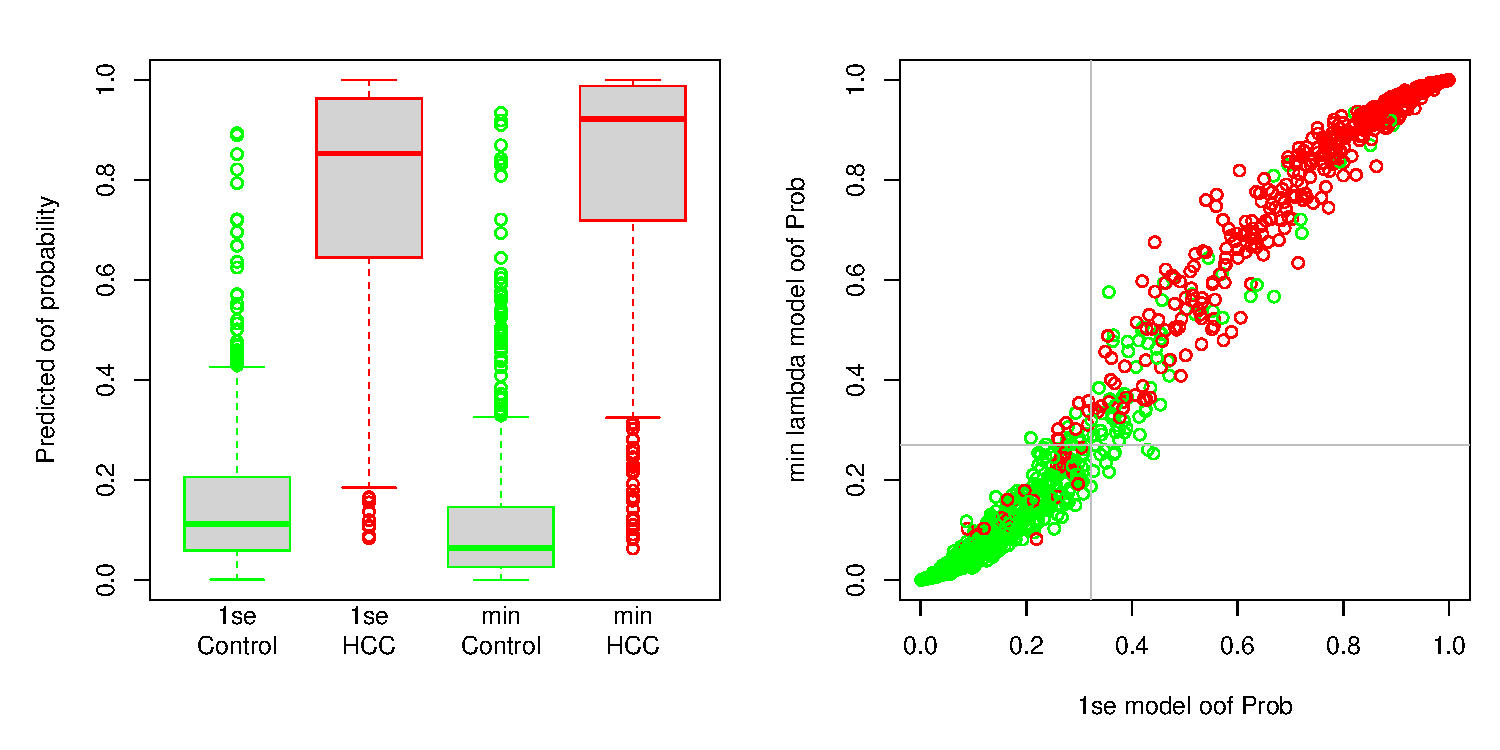
\includegraphics{Static/figures/enet-get-sample-pred-1.pdf}
\caption{\label{fig:enet-get-sample-pred}Predicted probabilities - averaged over cv replicates}
\end{figure}

We see that there isn't a big difference in out-of-fold predicted
probabilities between the one-standard-error rule ans minimum lamda models.
One way to quantify
the difference in classification errors is to classify samples
according to each vector of predicted probabilities, setting
the thresholds to achieve a fixed false positive rate, 10\% say.
These thresholds are indicated by the grey lines in the scatter plot
on the right side of Figure \ref{fig:get-sample-pred}.

\begin{Shaded}
\begin{Highlighting}[]
\NormalTok{enetAll\_predClass\_1se\_vec <{-}}\StringTok{ }\KeywordTok{ifelse}\NormalTok{(}
\NormalTok{ enetAll\_predResp\_1se\_vec }\OperatorTok{>}\StringTok{ }\NormalTok{thres\_1se, }\StringTok{\textquotesingle{}HCC\textquotesingle{}}\NormalTok{, }\StringTok{\textquotesingle{}Control\textquotesingle{}}\NormalTok{)}

\NormalTok{enetAll\_predClass\_min\_vec <{-}}\StringTok{ }\KeywordTok{ifelse}\NormalTok{(}
\NormalTok{ enetAll\_predResp\_min\_vec }\OperatorTok{>}\StringTok{ }\NormalTok{thres\_min, }\StringTok{\textquotesingle{}HCC\textquotesingle{}}\NormalTok{, }\StringTok{\textquotesingle{}Control\textquotesingle{}}\NormalTok{)}

\NormalTok{tmp <{-}}\StringTok{ }\KeywordTok{cbind}\NormalTok{(}
 \KeywordTok{table}\NormalTok{(}\DataTypeTok{truth=}\NormalTok{all\_group\_vec, }\StringTok{\textasciigrave{}}\DataTypeTok{1se{-}pred}\StringTok{\textasciigrave{}}\NormalTok{=enetAll\_predClass\_1se\_vec),}
 \KeywordTok{table}\NormalTok{(}\DataTypeTok{truth=}\NormalTok{all\_group\_vec, }\StringTok{\textasciigrave{}}\DataTypeTok{min{-}pred}\StringTok{\textasciigrave{}}\NormalTok{=enetAll\_predClass\_min\_vec)}
\NormalTok{) }
\CommentTok{\# Hack for printing}
\KeywordTok{colnames}\NormalTok{(tmp) <{-}}\StringTok{ }\KeywordTok{c}\NormalTok{(}\StringTok{\textquotesingle{}1se{-}Control\textquotesingle{}}\NormalTok{, }\StringTok{\textquotesingle{}1se{-}HCC\textquotesingle{}}\NormalTok{, }\StringTok{\textquotesingle{}min{-}Control\textquotesingle{}}\NormalTok{, }\StringTok{\textquotesingle{}min{-}HCC\textquotesingle{}}\NormalTok{)}

\NormalTok{knitr}\OperatorTok{::}\KeywordTok{kable}\NormalTok{(tmp,}
  \DataTypeTok{caption =} \StringTok{"Classifications: rows are truth"}\NormalTok{,}
  \DataTypeTok{digits=}\DecValTok{1}\NormalTok{) }\OperatorTok{\%>\%}
\StringTok{   }\NormalTok{kableExtra}\OperatorTok{::}\KeywordTok{kable\_styling}\NormalTok{(}\DataTypeTok{full\_width =}\NormalTok{ F)}
\end{Highlighting}
\end{Shaded}

\begin{table}

\caption{\label{tab:enet-get-sample-class}Classifications: rows are truth}
\centering
\begin{tabular}[t]{l|r|r|r|r}
\hline
  & 1se-Control & 1se-HCC & min-Control & min-HCC\\
\hline
Control & 700 & 78 & 700 & 78\\
\hline
HCC & 34 & 521 & 25 & 530\\
\hline
\end{tabular}
\end{table}

When we fix the false positive rate at 10\%, the \texttt{1se} model makes 39 false
negative calls whereas the minimum lambda model makes 32. A difference
of \(1.3\)\%

\hypertarget{selected-feature-list-stability-1}{%
\section*{Selected feature list stability}\label{selected-feature-list-stability-1}}
\addcontentsline{toc}{section}{Selected feature list stability}

Before moving on to the simulation, let's examine gene selection stability on the
full data set. We have two sets of sellected features - one for the
one standard deviation rile model, and one for the mimimum lambda model.
We saw in Table \ref{tab:model-size-enetAll} that the number of features
selected by the minimum lambda models had an IQR of
\(271.5-457.25\),
while the one standard error rule models had an IQR of
\(174-215\).

Let's examine the stability of the gene lists across cv replicates.

\begin{Shaded}
\begin{Highlighting}[]
\CommentTok{\#\#\# CLEAR CACHE}


\CommentTok{\# 1se}
\NormalTok{enetAll\_coef\_1se\_lst <{-}}\StringTok{ }\KeywordTok{lapply}\NormalTok{(cv\_enetAll\_lst, }\ControlFlowTok{function}\NormalTok{(cv\_fit)\{}
\NormalTok{ cv\_fit\_coef <{-}}\StringTok{ }\KeywordTok{coef}\NormalTok{(}
\NormalTok{ cv\_fit,}
 \DataTypeTok{s =} \StringTok{"lambda.1se"}
\NormalTok{ )}
\NormalTok{ cv\_fit\_coef}\OperatorTok{@}\NormalTok{Dimnames[[}\DecValTok{1}\NormalTok{]][cv\_fit\_coef}\OperatorTok{@}\NormalTok{i[}\OperatorTok{{-}}\DecValTok{1}\NormalTok{]]}
\NormalTok{ \})}

\CommentTok{\# put into matrix}
\NormalTok{enetAll\_coef\_1se\_all <{-}}\StringTok{ }\KeywordTok{Reduce}\NormalTok{(union, enetAll\_coef\_1se\_lst)}
\NormalTok{enetAll\_coef\_1se\_mtx <{-}}\StringTok{ }\KeywordTok{sapply}\NormalTok{(enetAll\_coef\_1se\_lst, }
  \ControlFlowTok{function}\NormalTok{(LL) }\KeywordTok{is.element}\NormalTok{(enetAll\_coef\_1se\_all, LL)}
\NormalTok{)}
\KeywordTok{rownames}\NormalTok{(enetAll\_coef\_1se\_mtx) <{-}}\StringTok{ }\NormalTok{enetAll\_coef\_1se\_all}

\NormalTok{genes\_by\_rep\_1se\_tbl <{-}}\StringTok{ }\KeywordTok{table}\NormalTok{(}\KeywordTok{rowSums}\NormalTok{(enetAll\_coef\_1se\_mtx))}
\KeywordTok{barplot}\NormalTok{(}
\NormalTok{ genes\_by\_rep\_1se\_tbl,}
 \DataTypeTok{xlab=}\StringTok{\textquotesingle{}Number of Replicates\textquotesingle{}}\NormalTok{,}
 \DataTypeTok{ylab=}\StringTok{\textquotesingle{}Number of features\textquotesingle{}}

\NormalTok{)}
\end{Highlighting}
\end{Shaded}

\begin{figure}
\centering
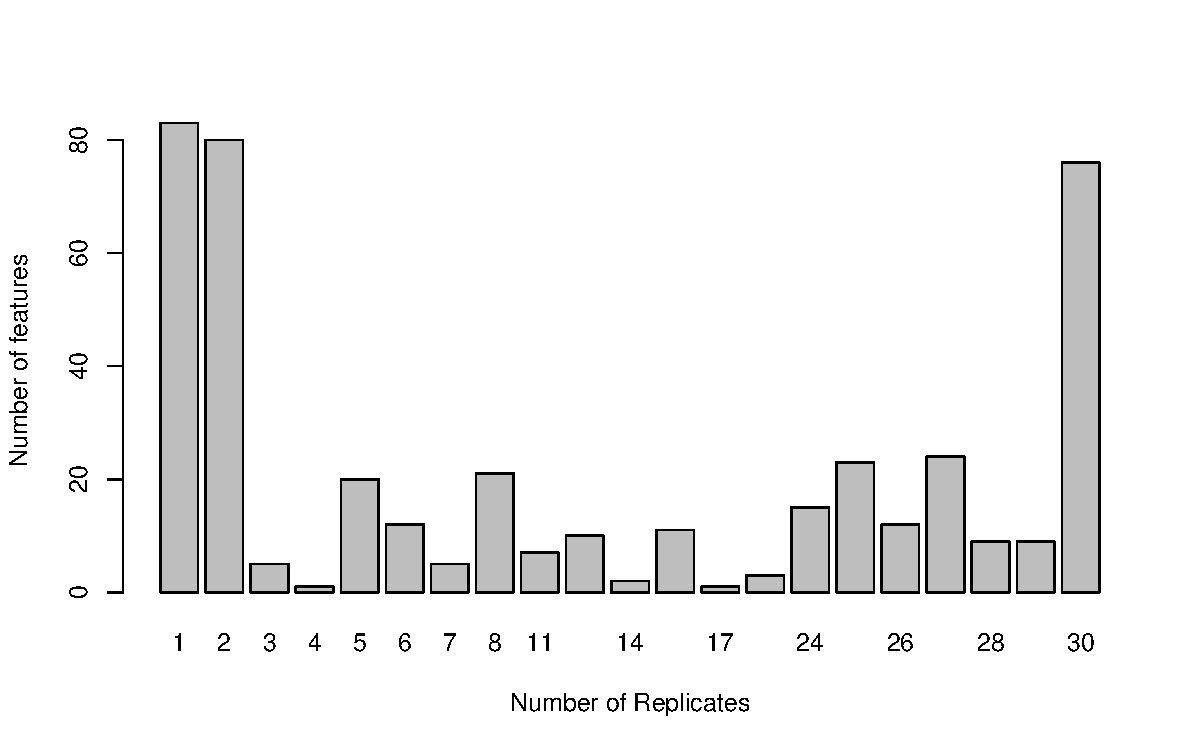
\includegraphics{Static/figures/enet-feature-list-1se-1.pdf}
\caption{\label{fig:enet-feature-list-1se}Feature list stability for one standard error rule models}
\end{figure}

We see that \(76\) features are included in every
cv replicate. These make up between
\(35\)\%
and
\(44\)\%
(Q1 and Q3) of the cv replicate one standard error rule models feature lists.

\begin{Shaded}
\begin{Highlighting}[]
\CommentTok{\#\#\# CLEAR CACHE}


\CommentTok{\# min}
\NormalTok{enetAll\_coef\_min\_lst <{-}}\StringTok{ }\KeywordTok{lapply}\NormalTok{(cv\_enetAll\_lst, }\ControlFlowTok{function}\NormalTok{(cv\_fit)\{}
\NormalTok{ cv\_fit\_coef <{-}}\StringTok{ }\KeywordTok{coef}\NormalTok{(}
\NormalTok{ cv\_fit,}
 \DataTypeTok{s =} \StringTok{"lambda.min"}
\NormalTok{ )}
\NormalTok{ cv\_fit\_coef}\OperatorTok{@}\NormalTok{Dimnames[[}\DecValTok{1}\NormalTok{]][cv\_fit\_coef}\OperatorTok{@}\NormalTok{i[}\OperatorTok{{-}}\DecValTok{1}\NormalTok{]]}
\NormalTok{ \})}

\CommentTok{\# put into matrix}
\NormalTok{enetAll\_coef\_min\_all <{-}}\StringTok{ }\KeywordTok{Reduce}\NormalTok{(union, enetAll\_coef\_min\_lst)}
\NormalTok{enetAll\_coef\_min\_mtx <{-}}\StringTok{ }\KeywordTok{sapply}\NormalTok{(enetAll\_coef\_min\_lst, }
  \ControlFlowTok{function}\NormalTok{(LL) }\KeywordTok{is.element}\NormalTok{(enetAll\_coef\_min\_all, LL)}
\NormalTok{)}
\KeywordTok{rownames}\NormalTok{(enetAll\_coef\_min\_mtx) <{-}}\StringTok{ }\NormalTok{enetAll\_coef\_min\_all}

\NormalTok{genes\_by\_rep\_min\_tbl <{-}}\StringTok{ }\KeywordTok{table}\NormalTok{(}\KeywordTok{rowSums}\NormalTok{(enetAll\_coef\_min\_mtx))}
\KeywordTok{barplot}\NormalTok{(}
\NormalTok{ genes\_by\_rep\_min\_tbl,}
 \DataTypeTok{xlab=}\StringTok{\textquotesingle{}Number of Replicates\textquotesingle{}}\NormalTok{,}
 \DataTypeTok{ylab=}\StringTok{\textquotesingle{}Number of features\textquotesingle{}}

\NormalTok{)}
\end{Highlighting}
\end{Shaded}

\begin{figure}
\centering
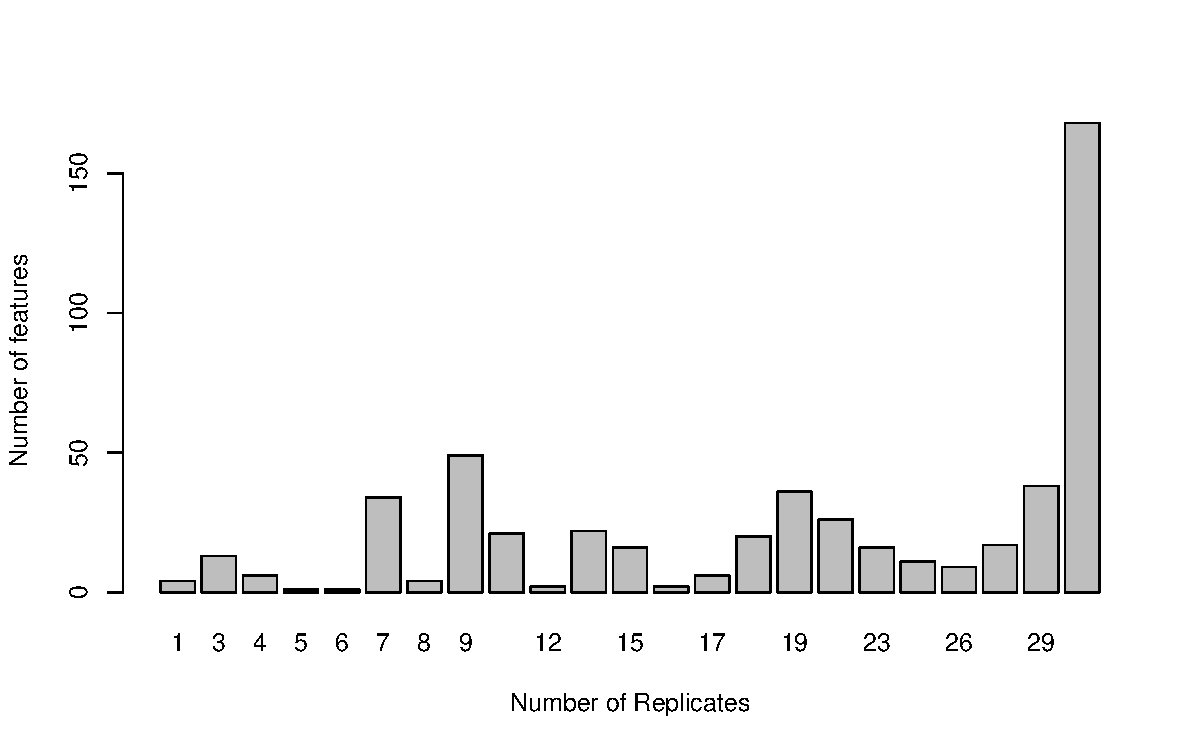
\includegraphics{Static/figures/enet-feature-list-min-1.pdf}
\caption{\label{fig:enet-feature-list-min}Feature list stability for minimum lambda models}
\end{figure}

We see that \(168\) features are included in every
cv replicate. These make up between
\(37\)\%
and
\(62\)\%
(Q1 and Q3) of the cv replicate min feature lists.
We will consider the genes that are selected in all cv replicates as a
gene signature produced by each model.

\begin{Shaded}
\begin{Highlighting}[]
\NormalTok{enet\_gene\_sign\_1se\_vec <{-}}\StringTok{ }\KeywordTok{rownames}\NormalTok{(enetAll\_coef\_1se\_mtx)[}\KeywordTok{rowSums}\NormalTok{(enetAll\_coef\_1se\_mtx)}\OperatorTok{==}\DecValTok{30}\NormalTok{]}
\NormalTok{enet\_gene\_sign\_min\_vec <{-}}\StringTok{ }\KeywordTok{rownames}\NormalTok{(enetAll\_coef\_min\_mtx)[}\KeywordTok{rowSums}\NormalTok{(enetAll\_coef\_min\_mtx)}\OperatorTok{==}\DecValTok{30}\NormalTok{]}
\end{Highlighting}
\end{Shaded}

76 out of
76 of the genes in the 1se model gene signature
are contained in the min lambda model gene signature.

\hypertarget{run-simulations---enet}{%
\section*{Run simulations - enet}\label{run-simulations---enet}}
\addcontentsline{toc}{section}{Run simulations - enet}

As these make take a while to run,
we will save the results of each similation to a different
object and store to disk. These can be easily read from disk
when needed for analysis.

The simulation saves results to the file system and
only needs to be run once. The simulation takes \(\approx\) 8 minutes
per iteration, or 4 hours of run time on a laptop.
(Platform: x86\_64-apple-darwin17.0 (64-bit)
Running under: macOS Mojave 10.14.6)

\begin{Shaded}
\begin{Highlighting}[]
\CommentTok{\#\#\# CLEAR CACHE}
\NormalTok{start\_time <{-}}\StringTok{ }\KeywordTok{proc.time}\NormalTok{()}

\CommentTok{\# Get stage from SIZE}
\NormalTok{stage\_vec <{-}}\StringTok{ }\KeywordTok{cut}\NormalTok{(}\DecValTok{1}\OperatorTok{:}\KeywordTok{nrow}\NormalTok{(sim\_control\_qual\_mtx), }\KeywordTok{c}\NormalTok{(}\DecValTok{0}\NormalTok{, SIZE), }\DataTypeTok{include.lowest =}\NormalTok{ T)}

\CommentTok{\# ran in two runs 1:7, 8:ncol}
\ControlFlowTok{for}\NormalTok{ (SIMno }\ControlFlowTok{in} \DecValTok{8}\OperatorTok{:}\KeywordTok{ncol}\NormalTok{(sim\_control\_qual\_mtx)) \{}

  \CommentTok{\#cat("Running simulation ", SIMno, "\textbackslash{}n")}

\NormalTok{  sim\_cv\_lst <{-}}\StringTok{ }\KeywordTok{lapply}\NormalTok{(}\DecValTok{1}\OperatorTok{:}\KeywordTok{length}\NormalTok{(}\KeywordTok{levels}\NormalTok{(stage\_vec)), }\ControlFlowTok{function}\NormalTok{(STGno) \{}
\NormalTok{    Stage\_rows\_vec <{-}}\StringTok{ }\KeywordTok{which}\NormalTok{(stage\_vec }\OperatorTok{\%in\%}\StringTok{ }\KeywordTok{levels}\NormalTok{(stage\_vec)[}\DecValTok{1}\OperatorTok{:}\NormalTok{STGno])}
    \CommentTok{\#cat("Stage ", STGno, "{-} analyzing", length(Stage\_rows\_vec), "paired samples.\textbackslash{}n")}

\NormalTok{    sim\_stage\_samples\_vec <{-}}\StringTok{ }\KeywordTok{c}\NormalTok{(}
\NormalTok{      all\_control\_vec[sim\_control\_mtx[Stage\_rows\_vec, SIMno]],}
\NormalTok{      all\_affected\_vec[sim\_affected\_mtx[Stage\_rows\_vec, SIMno]]}
\NormalTok{    )}
\NormalTok{    sim\_stage\_lcpm\_mtx <{-}}\StringTok{ }\NormalTok{all\_lcpm\_mtx[sim\_stage\_samples\_vec, ]}
\NormalTok{    sim\_stage\_group\_vec <{-}}\StringTok{ }\NormalTok{all\_group\_vec[sim\_stage\_samples\_vec]}
    \CommentTok{\#print(table(sim\_stage\_group\_vec))}

\NormalTok{    sim\_stage\_cv\_lst <{-}}\StringTok{ }\KeywordTok{lapply}\NormalTok{(}\DecValTok{1}\OperatorTok{:}\NormalTok{CV\_REP, }\ControlFlowTok{function}\NormalTok{(CV) \{}
\NormalTok{      cv\_fit <{-}}\StringTok{ }\NormalTok{glmnet}\OperatorTok{::}\KeywordTok{cv.glmnet}\NormalTok{(}
        \DataTypeTok{x =}\NormalTok{ sim\_stage\_lcpm\_mtx,}
        \DataTypeTok{y =}\NormalTok{ sim\_stage\_group\_vec,}
        \DataTypeTok{alpha =} \DecValTok{1}\NormalTok{,}
        \DataTypeTok{family =} \StringTok{"binomial"}\NormalTok{,}
        \DataTypeTok{type.measure =} \StringTok{"class"}\NormalTok{,}
        \DataTypeTok{keep =}\NormalTok{ T,}
        \DataTypeTok{nlambda =} \DecValTok{30}
\NormalTok{      )}

      \CommentTok{\# Extract 1se metrics from cv\_fit}
      \CommentTok{\#\#\#\#\#\#\#\#\#\#\#\#\#\#\#\#\#\#\#\#\#\#\#}
\NormalTok{      ndx\_1se <{-}}\StringTok{ }\KeywordTok{which}\NormalTok{(cv\_fit}\OperatorTok{$}\NormalTok{lambda }\OperatorTok{==}\StringTok{ }\NormalTok{cv\_fit}\OperatorTok{$}\NormalTok{lambda}\FloatTok{.1}\NormalTok{se)}

\NormalTok{      nzero\_1se <{-}}\StringTok{ }\NormalTok{cv\_fit}\OperatorTok{$}\NormalTok{nzero[ndx\_1se]}
\NormalTok{      cvm\_1se <{-}}\StringTok{ }\NormalTok{cv\_fit}\OperatorTok{$}\NormalTok{cvm[ndx\_1se]}

      \CommentTok{\# test error}
\NormalTok{      sim\_stage\_test\_samples\_vec <{-}}\StringTok{ }\KeywordTok{setdiff}\NormalTok{(}\KeywordTok{rownames}\NormalTok{(all\_lcpm\_mtx), sim\_stage\_samples\_vec)}
\NormalTok{      sim\_stage\_test\_lcpm\_mtx <{-}}\StringTok{ }\NormalTok{all\_lcpm\_mtx[sim\_stage\_test\_samples\_vec,]}
\NormalTok{      sim\_stage\_test\_group\_vec <{-}}\StringTok{ }\NormalTok{all\_group\_vec[sim\_stage\_test\_samples\_vec]}

\NormalTok{      test\_pred\_1se\_vec <{-}}\StringTok{ }\KeywordTok{predict}\NormalTok{(}
\NormalTok{       cv\_fit,}
       \DataTypeTok{newx=}\NormalTok{sim\_stage\_test\_lcpm\_mtx,}
       \DataTypeTok{s=}\StringTok{"lambda.1se"}\NormalTok{,}
       \DataTypeTok{type=}\StringTok{"class"}
\NormalTok{      )}
\NormalTok{      test\_1se\_error <{-}}\StringTok{ }\KeywordTok{mean}\NormalTok{(test\_pred\_1se\_vec }\OperatorTok{!=}\StringTok{ }\NormalTok{sim\_stage\_test\_group\_vec)}

      \CommentTok{\# genes}
\NormalTok{      coef\_1se <{-}}\StringTok{ }\KeywordTok{coef}\NormalTok{(}
\NormalTok{        cv\_fit,}
        \DataTypeTok{s =} \StringTok{"lambda.1se"}
\NormalTok{      )}
\NormalTok{      genes\_1se <{-}}\StringTok{ }\NormalTok{coef\_1se}\OperatorTok{@}\NormalTok{Dimnames[[}\DecValTok{1}\NormalTok{]][coef\_1se}\OperatorTok{@}\NormalTok{i[}\OperatorTok{{-}}\DecValTok{1}\NormalTok{]]}

      \CommentTok{\# Extract min metrics from cv\_fit}
      \CommentTok{\#\#\#\#\#\#\#\#\#\#\#\#\#\#\#\#\#\#\#\#\#\#\#}
\NormalTok{      ndx\_min <{-}}\StringTok{ }\KeywordTok{which}\NormalTok{(cv\_fit}\OperatorTok{$}\NormalTok{lambda }\OperatorTok{==}\StringTok{ }\NormalTok{cv\_fit}\OperatorTok{$}\NormalTok{lambda.min)}

\NormalTok{      nzero\_min <{-}}\StringTok{ }\NormalTok{cv\_fit}\OperatorTok{$}\NormalTok{nzero[ndx\_min]}
\NormalTok{      cvm\_min <{-}}\StringTok{ }\NormalTok{cv\_fit}\OperatorTok{$}\NormalTok{cvm[ndx\_min]}

      \CommentTok{\# test error}
\NormalTok{      sim\_stage\_test\_samples\_vec <{-}}\StringTok{ }\KeywordTok{setdiff}\NormalTok{(}\KeywordTok{rownames}\NormalTok{(all\_lcpm\_mtx), sim\_stage\_samples\_vec)}
\NormalTok{      sim\_stage\_test\_lcpm\_mtx <{-}}\StringTok{ }\NormalTok{all\_lcpm\_mtx[sim\_stage\_test\_samples\_vec,]}
\NormalTok{      sim\_stage\_test\_group\_vec <{-}}\StringTok{ }\NormalTok{all\_group\_vec[sim\_stage\_test\_samples\_vec]}

\NormalTok{      test\_pred\_min\_vec <{-}}\StringTok{ }\KeywordTok{predict}\NormalTok{(}
\NormalTok{       cv\_fit,}
       \DataTypeTok{newx=}\NormalTok{sim\_stage\_test\_lcpm\_mtx,}
       \DataTypeTok{s=}\StringTok{"lambda.min"}\NormalTok{,}
       \DataTypeTok{type=}\StringTok{"class"}
\NormalTok{      )}
\NormalTok{      test\_min\_error <{-}}\StringTok{ }\KeywordTok{mean}\NormalTok{(test\_pred\_min\_vec }\OperatorTok{!=}\StringTok{ }\NormalTok{sim\_stage\_test\_group\_vec)}

      \CommentTok{\# genes}
\NormalTok{      coef\_min <{-}}\StringTok{ }\KeywordTok{coef}\NormalTok{(}
\NormalTok{        cv\_fit,}
        \DataTypeTok{s =} \StringTok{"lambda.min"}
\NormalTok{      )}
\NormalTok{      genes\_min <{-}}\StringTok{ }\NormalTok{coef\_min}\OperatorTok{@}\NormalTok{Dimnames[[}\DecValTok{1}\NormalTok{]][coef\_min}\OperatorTok{@}\NormalTok{i[}\OperatorTok{{-}}\DecValTok{1}\NormalTok{]]}

      \CommentTok{\# return cv\_fit summary metrics}
      \KeywordTok{list}\NormalTok{(}
       \DataTypeTok{p\_1se =}\NormalTok{ nzero\_1se, }
       \DataTypeTok{p\_min =}\NormalTok{ nzero\_min, }
       \DataTypeTok{cv\_1se =}\NormalTok{ cvm\_1se, }
       \DataTypeTok{cv\_min =}\NormalTok{ cvm\_min, }
       \DataTypeTok{test\_1se=}\NormalTok{test\_1se\_error, }
       \DataTypeTok{test\_min=}\NormalTok{test\_min\_error, }
       \DataTypeTok{genes\_1se =}\NormalTok{ genes\_1se,}
       \DataTypeTok{genes\_min =}\NormalTok{ genes\_min)}
\NormalTok{    \})}
\NormalTok{    sim\_stage\_cv\_lst}
\NormalTok{  \})}

  \CommentTok{\# save  sim\_cv\_lst}
\NormalTok{  fName <{-}}\StringTok{ }\KeywordTok{paste0}\NormalTok{(}\StringTok{"enet\_sim\_"}\NormalTok{, SIMno, }\StringTok{"\_cv\_lst"}\NormalTok{)}
  \KeywordTok{assign}\NormalTok{(fName, sim\_cv\_lst)}
  \KeywordTok{save}\NormalTok{(}\DataTypeTok{list =}\NormalTok{ fName, }\DataTypeTok{file=}\KeywordTok{file.path}\NormalTok{(}\StringTok{"RData"}\NormalTok{, fName))}

\NormalTok{\}}
  \KeywordTok{message}\NormalTok{(}\StringTok{"simulation time: "}\NormalTok{, }\KeywordTok{round}\NormalTok{((}\KeywordTok{proc.time}\NormalTok{() }\OperatorTok{{-}}\StringTok{ }\NormalTok{start\_time)[}\DecValTok{3}\NormalTok{], }\DecValTok{2}\NormalTok{), }\StringTok{"s"}\NormalTok{)}
\end{Highlighting}
\end{Shaded}

\hypertarget{enet-simulation-results}{%
\section*{enet Simulation results}\label{enet-simulation-results}}
\addcontentsline{toc}{section}{enet Simulation results}

\hypertarget{simulation-results---look-at-one-simulation-1}{%
\subsection*{Simulation Results - look at one simulation}\label{simulation-results---look-at-one-simulation-1}}
\addcontentsline{toc}{subsection}{Simulation Results - look at one simulation}

First examine results for one simulation run.

\begin{Shaded}
\begin{Highlighting}[]
\CommentTok{\#\#\# CLEAR CACHE}

\CommentTok{\# get full model cv error ref}
\NormalTok{error\_1se\_vec <{-}}\StringTok{ }\KeywordTok{sapply}\NormalTok{(cv\_enetAll\_lst,}
 \ControlFlowTok{function}\NormalTok{(cv\_fit) cv\_fit}\OperatorTok{$}\NormalTok{cvm[cv\_fit}\OperatorTok{$}\NormalTok{lambda }\OperatorTok{==}\StringTok{ }\NormalTok{cv\_fit}\OperatorTok{$}\NormalTok{lambda}\FloatTok{.1}\NormalTok{se])}
\NormalTok{error\_1se\_q2 <{-}}\StringTok{ }\KeywordTok{quantile}\NormalTok{(error\_1se\_vec, }\DataTypeTok{prob=}\DecValTok{1}\OperatorTok{/}\DecValTok{2}\NormalTok{)        }

\NormalTok{error\_min\_vec <{-}}\StringTok{ }\KeywordTok{sapply}\NormalTok{(cv\_enetAll\_lst,}
 \ControlFlowTok{function}\NormalTok{(cv\_fit) cv\_fit}\OperatorTok{$}\NormalTok{cvm[cv\_fit}\OperatorTok{$}\NormalTok{lambda }\OperatorTok{==}\StringTok{ }\NormalTok{cv\_fit}\OperatorTok{$}\NormalTok{lambda.min])}
\NormalTok{error\_min\_q2 <{-}}\StringTok{ }\KeywordTok{quantile}\NormalTok{(error\_min\_vec, }\DataTypeTok{prob=}\DecValTok{1}\OperatorTok{/}\DecValTok{2}\NormalTok{)        }

\CommentTok{\# Utility objects}
\NormalTok{SIZE0 <{-}}\StringTok{ }\NormalTok{stringr}\OperatorTok{::}\KeywordTok{str\_pad}\NormalTok{(SIZE, }\DataTypeTok{width=}\DecValTok{3}\NormalTok{, }\DataTypeTok{pad=}\StringTok{\textquotesingle{}0\textquotesingle{}}\NormalTok{)}
\NormalTok{stage\_vec <{-}}\StringTok{ }\KeywordTok{cut}\NormalTok{(}\DecValTok{1}\OperatorTok{:}\KeywordTok{nrow}\NormalTok{(sim\_control\_qual\_mtx), }\KeywordTok{c}\NormalTok{(}\DecValTok{0}\NormalTok{,SIZE), }\DataTypeTok{include.lowest =}\NormalTok{ T)}


\CommentTok{\#SIM <{-} "Sim\_01"}

\ControlFlowTok{for}\NormalTok{(SIM }\ControlFlowTok{in} \KeywordTok{unique}\NormalTok{(enet\_sim\_results\_frm}\OperatorTok{$}\NormalTok{SimNo)[}\DecValTok{1}\NormalTok{])\{}

\NormalTok{SimNum <{-}}\StringTok{ }\KeywordTok{as.numeric}\NormalTok{(}\KeywordTok{sub}\NormalTok{(}\StringTok{\textquotesingle{}Sim\_\textquotesingle{}}\NormalTok{,}\StringTok{\textquotesingle{}\textquotesingle{}}\NormalTok{,SIM))}

\NormalTok{simNo\_results\_frm <{-}}\StringTok{ }\NormalTok{enet\_sim\_results\_frm }\OperatorTok{\%>\%}\StringTok{ }\NormalTok{dplyr}\OperatorTok{::}\KeywordTok{filter}\NormalTok{(SimNo}\OperatorTok{==}\NormalTok{SIM)}


\CommentTok{\# errors}
\KeywordTok{par}\NormalTok{(}\DataTypeTok{mfrow=}\KeywordTok{c}\NormalTok{(}\DecValTok{1}\NormalTok{,}\DecValTok{2}\NormalTok{), }\DataTypeTok{mar=}\KeywordTok{c}\NormalTok{(}\DecValTok{4}\NormalTok{, }\DecValTok{2}\NormalTok{, }\DecValTok{2}\NormalTok{, }\DecValTok{1}\NormalTok{), }\DataTypeTok{oma=}\KeywordTok{c}\NormalTok{(}\DecValTok{0}\NormalTok{,}\DecValTok{0}\NormalTok{,}\DecValTok{2}\NormalTok{,}\DecValTok{0}\NormalTok{))}
\CommentTok{\#\#\#\#\#\#\#\#\#\#\#\#\#\#\#\#\#\#\#}
\CommentTok{\# 1se}
\CommentTok{\#\#\#\#\#\#\#\#\#\#\#\#\#\#\#\#\#\#\#\#}
\NormalTok{cv\_1se\_lst <{-}}\StringTok{ }\KeywordTok{with}\NormalTok{(simNo\_results\_frm,}
 \KeywordTok{split}\NormalTok{(cv\_1se, Size))}
\KeywordTok{names}\NormalTok{(cv\_1se\_lst) <{-}}\StringTok{ }\KeywordTok{paste0}\NormalTok{(stringr}\OperatorTok{::}\KeywordTok{str\_pad}\NormalTok{(}\KeywordTok{names}\NormalTok{(cv\_1se\_lst), }\DataTypeTok{width=}\DecValTok{3}\NormalTok{, }\DataTypeTok{pad=}\StringTok{\textquotesingle{}0\textquotesingle{}}\NormalTok{),}\StringTok{\textquotesingle{}\_cv\textquotesingle{}}\NormalTok{)}

\NormalTok{test\_1se\_lst <{-}}\StringTok{ }\KeywordTok{with}\NormalTok{(simNo\_results\_frm,}
 \KeywordTok{split}\NormalTok{(test\_1se, Size))}
\KeywordTok{names}\NormalTok{(test\_1se\_lst) <{-}}\StringTok{ }\KeywordTok{paste0}\NormalTok{(stringr}\OperatorTok{::}\KeywordTok{str\_pad}\NormalTok{(}\KeywordTok{names}\NormalTok{(test\_1se\_lst), }\DataTypeTok{width=}\DecValTok{3}\NormalTok{, }\DataTypeTok{pad=}\StringTok{\textquotesingle{}0\textquotesingle{}}\NormalTok{),}\StringTok{\textquotesingle{}\_cv\textquotesingle{}}\NormalTok{)}

\NormalTok{error\_1se\_lst <{-}}\StringTok{ }\KeywordTok{c}\NormalTok{(cv\_1se\_lst, test\_1se\_lst)}
\NormalTok{error\_1se\_lst <{-}}\StringTok{ }\NormalTok{error\_1se\_lst[}\KeywordTok{order}\NormalTok{(}\KeywordTok{names}\NormalTok{(error\_1se\_lst))]}

\KeywordTok{boxplot}\NormalTok{(error\_1se\_lst, }
  \DataTypeTok{border=}\KeywordTok{c}\NormalTok{(}\StringTok{\textquotesingle{}blue\textquotesingle{}}\NormalTok{,}\StringTok{\textquotesingle{}green\textquotesingle{}}\NormalTok{), }
  \DataTypeTok{ylim=}\KeywordTok{c}\NormalTok{(}\FloatTok{0.05}\NormalTok{, }\FloatTok{.4}\NormalTok{),}
  \DataTypeTok{xaxt=}\StringTok{\textquotesingle{}n\textquotesingle{}}
\NormalTok{)}
\NormalTok{LL <{-}}\StringTok{ }\DecValTok{{-}1}
\KeywordTok{axis}\NormalTok{(}\DataTypeTok{side=}\DecValTok{1}\NormalTok{, }\DataTypeTok{tick=}\NormalTok{F, }\DataTypeTok{line =}\NormalTok{ LL,}
  \DataTypeTok{at =} \KeywordTok{match}\NormalTok{(}\KeywordTok{paste0}\NormalTok{(SIZE0,}\StringTok{\textquotesingle{}\_cv\textquotesingle{}}\NormalTok{),}\KeywordTok{names}\NormalTok{(error\_1se\_lst)), }
\NormalTok{  SIZE0}
\NormalTok{ )}
\KeywordTok{abline}\NormalTok{(}\DataTypeTok{v=} \KeywordTok{match}\NormalTok{(}\KeywordTok{paste0}\NormalTok{(SIZE0,}\StringTok{\textquotesingle{}\_cv\textquotesingle{}}\NormalTok{),}\KeywordTok{names}\NormalTok{(error\_1se\_lst))[}\OperatorTok{{-}}\DecValTok{1}\NormalTok{] }\OperatorTok{{-}}\StringTok{ }\FloatTok{0.5}\NormalTok{, }\DataTypeTok{col=}\StringTok{\textquotesingle{}grey\textquotesingle{}}\NormalTok{)}
\KeywordTok{abline}\NormalTok{(}\DataTypeTok{h=}\NormalTok{ error\_1se\_q2, }\DataTypeTok{col =} \StringTok{\textquotesingle{}red\textquotesingle{}}\NormalTok{)}
\KeywordTok{legend}\NormalTok{(}\StringTok{\textquotesingle{}topright\textquotesingle{}}\NormalTok{, }
   \CommentTok{\#title=\textquotesingle{}1se errors\textquotesingle{}, title.col = \textquotesingle{}black\textquotesingle{},}
   \DataTypeTok{text.col =} \KeywordTok{c}\NormalTok{(}\StringTok{\textquotesingle{}blue\textquotesingle{}}\NormalTok{,}\StringTok{\textquotesingle{}green\textquotesingle{}}\NormalTok{),}
   \DataTypeTok{legend =} \KeywordTok{c}\NormalTok{(}\StringTok{\textquotesingle{}cv error\textquotesingle{}}\NormalTok{, }\StringTok{\textquotesingle{}test set\textquotesingle{}}\NormalTok{),}
   \DataTypeTok{bty=}\StringTok{\textquotesingle{}n\textquotesingle{}}
\NormalTok{ )}
\KeywordTok{title}\NormalTok{(}\KeywordTok{paste}\NormalTok{(}\StringTok{\textquotesingle{}one se lambda {-} error rates\textquotesingle{}}\NormalTok{))}

\NormalTok{SKIP  <{-}}\StringTok{ }\ControlFlowTok{function}\NormalTok{() \{}
\CommentTok{\# Add qual annotation}
\NormalTok{control\_qual\_vec <{-}}\StringTok{ }\KeywordTok{sapply}\NormalTok{(}\KeywordTok{split}\NormalTok{(sim\_control\_qual\_mtx[,SimNum], stage\_vec), median)}
\NormalTok{affected\_qual\_vec <{-}}\StringTok{ }\KeywordTok{sapply}\NormalTok{(}\KeywordTok{split}\NormalTok{(sim\_affected\_qual\_mtx[,SimNum], stage\_vec), median)}
\NormalTok{LL <{-}}\StringTok{ }\NormalTok{LL }\OperatorTok{+}\StringTok{ }\DecValTok{1}
\KeywordTok{axis}\NormalTok{(}\DataTypeTok{side=}\DecValTok{1}\NormalTok{, }\DataTypeTok{tick=}\NormalTok{F, }\DataTypeTok{line =}\NormalTok{ LL,}
  \DataTypeTok{at =} \KeywordTok{match}\NormalTok{(}\KeywordTok{paste0}\NormalTok{(SIZE0,}\StringTok{\textquotesingle{}\_cv\textquotesingle{}}\NormalTok{),}\KeywordTok{names}\NormalTok{(error\_1se\_lst)),}
  \KeywordTok{round}\NormalTok{(control\_qual\_vec, }\DecValTok{2}\NormalTok{)}
\NormalTok{ )}
\NormalTok{LL <{-}}\StringTok{ }\NormalTok{LL }\OperatorTok{+}\StringTok{ }\DecValTok{1}
\KeywordTok{axis}\NormalTok{(}\DataTypeTok{side=}\DecValTok{1}\NormalTok{, }\DataTypeTok{tick=}\NormalTok{F, }\DataTypeTok{line =}\NormalTok{ LL,}
  \DataTypeTok{at =} \KeywordTok{match}\NormalTok{(}\KeywordTok{paste0}\NormalTok{(SIZE0,}\StringTok{\textquotesingle{}\_cv\textquotesingle{}}\NormalTok{),}\KeywordTok{names}\NormalTok{(error\_1se\_lst)),}
  \KeywordTok{round}\NormalTok{(affected\_qual\_vec, }\DecValTok{2}\NormalTok{)}
\NormalTok{ )}
\NormalTok{\}}\CommentTok{\#SKIP}

\CommentTok{\# min}
\CommentTok{\#\#\#\#\#\#\#\#\#\#\#\#\#\#\#\#\#\#\#\#}
\NormalTok{cv\_min\_lst <{-}}\StringTok{ }\KeywordTok{with}\NormalTok{(simNo\_results\_frm,}
 \KeywordTok{split}\NormalTok{(cv\_min, Size))}
\KeywordTok{names}\NormalTok{(cv\_min\_lst) <{-}}\StringTok{ }\KeywordTok{paste0}\NormalTok{(stringr}\OperatorTok{::}\KeywordTok{str\_pad}\NormalTok{(}\KeywordTok{names}\NormalTok{(cv\_min\_lst), }\DataTypeTok{width=}\DecValTok{3}\NormalTok{, }\DataTypeTok{pad=}\StringTok{\textquotesingle{}0\textquotesingle{}}\NormalTok{),}\StringTok{\textquotesingle{}\_cv\textquotesingle{}}\NormalTok{)}

\NormalTok{test\_min\_lst <{-}}\StringTok{ }\KeywordTok{with}\NormalTok{(simNo\_results\_frm,}
 \KeywordTok{split}\NormalTok{(test\_min, Size))}
\KeywordTok{names}\NormalTok{(test\_min\_lst) <{-}}\StringTok{ }\KeywordTok{paste0}\NormalTok{(stringr}\OperatorTok{::}\KeywordTok{str\_pad}\NormalTok{(}\KeywordTok{names}\NormalTok{(test\_min\_lst), }\DataTypeTok{width=}\DecValTok{3}\NormalTok{, }\DataTypeTok{pad=}\StringTok{\textquotesingle{}0\textquotesingle{}}\NormalTok{),}\StringTok{\textquotesingle{}\_cv\textquotesingle{}}\NormalTok{)}

\NormalTok{error\_min\_lst <{-}}\StringTok{ }\KeywordTok{c}\NormalTok{(cv\_min\_lst, test\_min\_lst)}
\NormalTok{error\_min\_lst <{-}}\StringTok{ }\NormalTok{error\_min\_lst[}\KeywordTok{order}\NormalTok{(}\KeywordTok{names}\NormalTok{(error\_min\_lst))]}

\KeywordTok{boxplot}\NormalTok{(error\_min\_lst, }
  \DataTypeTok{border=}\KeywordTok{c}\NormalTok{(}\StringTok{\textquotesingle{}blue\textquotesingle{}}\NormalTok{,}\StringTok{\textquotesingle{}green\textquotesingle{}}\NormalTok{), }
  \DataTypeTok{ylim=}\KeywordTok{c}\NormalTok{(}\FloatTok{0.05}\NormalTok{, }\FloatTok{.4}\NormalTok{),}
  \DataTypeTok{xaxt=}\StringTok{\textquotesingle{}n\textquotesingle{}}
\NormalTok{)}
\NormalTok{LL <{-}}\StringTok{ }\DecValTok{{-}1}
\KeywordTok{axis}\NormalTok{(}\DataTypeTok{side=}\DecValTok{1}\NormalTok{, }\DataTypeTok{tick=}\NormalTok{F, }\DataTypeTok{line =}\NormalTok{ LL,}
  \DataTypeTok{at =} \KeywordTok{match}\NormalTok{(}\KeywordTok{paste0}\NormalTok{(SIZE0,}\StringTok{\textquotesingle{}\_cv\textquotesingle{}}\NormalTok{),}\KeywordTok{names}\NormalTok{(error\_min\_lst)), }
\NormalTok{  SIZE0}
\NormalTok{ )}
\KeywordTok{abline}\NormalTok{(}\DataTypeTok{v=} \KeywordTok{match}\NormalTok{(}\KeywordTok{paste0}\NormalTok{(SIZE0,}\StringTok{\textquotesingle{}\_cv\textquotesingle{}}\NormalTok{),}\KeywordTok{names}\NormalTok{(error\_min\_lst))[}\OperatorTok{{-}}\DecValTok{1}\NormalTok{] }\OperatorTok{{-}}\StringTok{ }\FloatTok{0.5}\NormalTok{, }\DataTypeTok{col=}\StringTok{\textquotesingle{}grey\textquotesingle{}}\NormalTok{)}
\KeywordTok{abline}\NormalTok{(}\DataTypeTok{h=}\NormalTok{ error\_min\_q2, }\DataTypeTok{col =} \StringTok{\textquotesingle{}red\textquotesingle{}}\NormalTok{)}
\KeywordTok{legend}\NormalTok{(}\StringTok{\textquotesingle{}topright\textquotesingle{}}\NormalTok{, }
   \CommentTok{\#title=\textquotesingle{}min errors\textquotesingle{}, title.col = \textquotesingle{}black\textquotesingle{},}
   \DataTypeTok{text.col =} \KeywordTok{c}\NormalTok{(}\StringTok{\textquotesingle{}blue\textquotesingle{}}\NormalTok{,}\StringTok{\textquotesingle{}green\textquotesingle{}}\NormalTok{),}
   \DataTypeTok{legend =} \KeywordTok{c}\NormalTok{(}\StringTok{\textquotesingle{}cv error\textquotesingle{}}\NormalTok{, }\StringTok{\textquotesingle{}test set\textquotesingle{}}\NormalTok{),}
   \DataTypeTok{bty=}\StringTok{\textquotesingle{}n\textquotesingle{}}
\NormalTok{ )}
\KeywordTok{title}\NormalTok{(}\KeywordTok{paste}\NormalTok{(}\StringTok{\textquotesingle{}min lambda {-} error rates\textquotesingle{}}\NormalTok{))}

\NormalTok{SKIP  <{-}}\StringTok{ }\ControlFlowTok{function}\NormalTok{() \{}
\CommentTok{\# Add qual annotation}
\NormalTok{control\_qual\_vec <{-}}\StringTok{ }\KeywordTok{sapply}\NormalTok{(}\KeywordTok{split}\NormalTok{(sim\_control\_qual\_mtx[,SimNum], stage\_vec), median)}
\NormalTok{affected\_qual\_vec <{-}}\StringTok{ }\KeywordTok{sapply}\NormalTok{(}\KeywordTok{split}\NormalTok{(sim\_affected\_qual\_mtx[,SimNum], stage\_vec), median)}
\NormalTok{LL <{-}}\StringTok{ }\NormalTok{LL }\OperatorTok{+}\StringTok{ }\DecValTok{1}
\KeywordTok{axis}\NormalTok{(}\DataTypeTok{side=}\DecValTok{1}\NormalTok{, }\DataTypeTok{tick=}\NormalTok{F, }\DataTypeTok{line =}\NormalTok{ LL,}
  \DataTypeTok{at =} \KeywordTok{match}\NormalTok{(}\KeywordTok{paste0}\NormalTok{(SIZE0,}\StringTok{\textquotesingle{}\_cv\textquotesingle{}}\NormalTok{),}\KeywordTok{names}\NormalTok{(error\_min\_lst)),}
  \KeywordTok{round}\NormalTok{(control\_qual\_vec, }\DecValTok{2}\NormalTok{)}
\NormalTok{ )}
\NormalTok{LL <{-}}\StringTok{ }\NormalTok{LL }\OperatorTok{+}\StringTok{ }\DecValTok{1}
\KeywordTok{axis}\NormalTok{(}\DataTypeTok{side=}\DecValTok{1}\NormalTok{, }\DataTypeTok{tick=}\NormalTok{F, }\DataTypeTok{line =}\NormalTok{ LL,}
  \DataTypeTok{at =} \KeywordTok{match}\NormalTok{(}\KeywordTok{paste0}\NormalTok{(SIZE0,}\StringTok{\textquotesingle{}\_cv\textquotesingle{}}\NormalTok{),}\KeywordTok{names}\NormalTok{(error\_min\_lst)),}
  \KeywordTok{round}\NormalTok{(affected\_qual\_vec, }\DecValTok{2}\NormalTok{)}
\NormalTok{ )}
\NormalTok{\}}\CommentTok{\#SKIP}
\KeywordTok{mtext}\NormalTok{(}\DataTypeTok{side=}\DecValTok{3}\NormalTok{, }\DataTypeTok{outer=}\NormalTok{T, }\DataTypeTok{cex=}\FloatTok{1.25}\NormalTok{, }\KeywordTok{paste}\NormalTok{(}\StringTok{\textquotesingle{}Sim =\textquotesingle{}}\NormalTok{,  SIM))}

\NormalTok{\} }\CommentTok{\# for(SIM}
\end{Highlighting}
\end{Shaded}

\begin{figure}
\centering
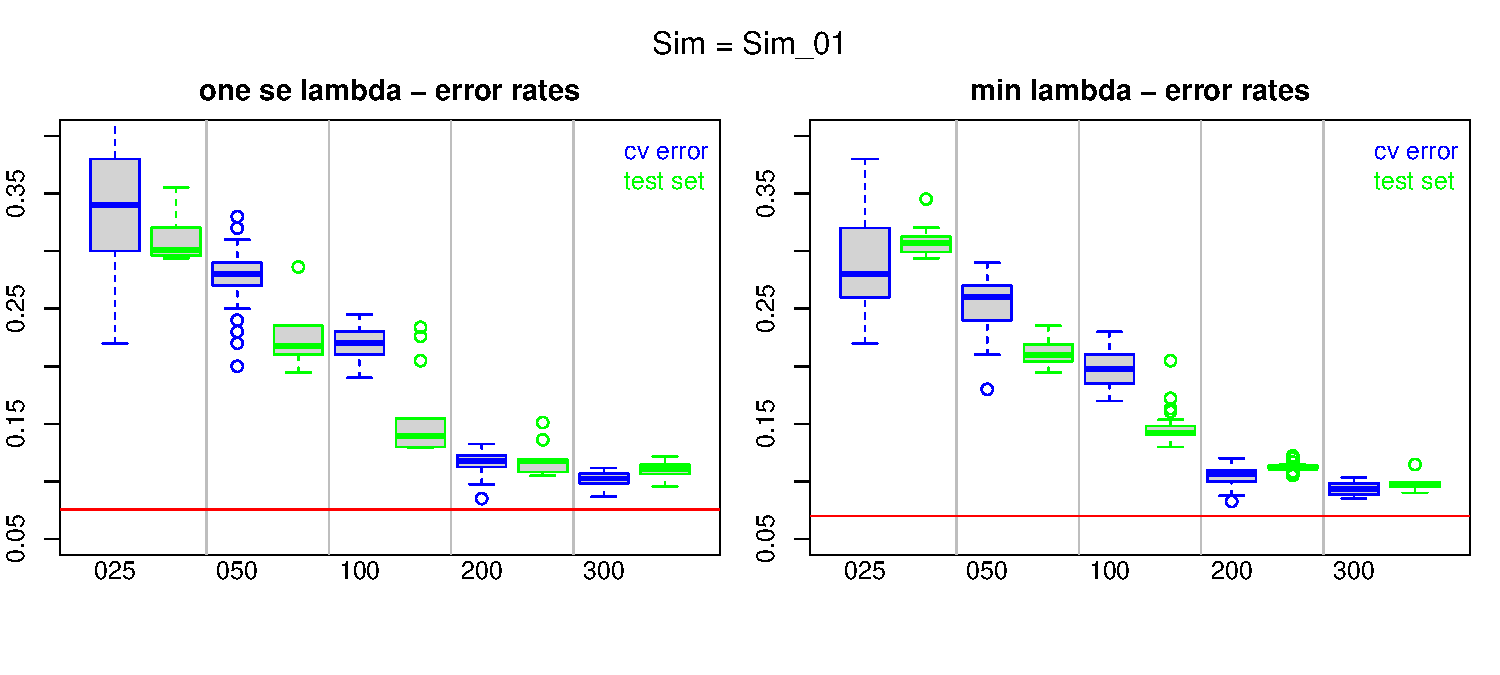
\includegraphics{Static/figures/enet-simRes-errors-bySim-1.pdf}
\caption{\label{fig:enet-simRes-errors-bySim}enet Model Errors by Sample Size}
\end{figure}

\begin{Shaded}
\begin{Highlighting}[]
\CommentTok{\#\#\# CLEAR CACHE}

\CommentTok{\# get full model nzero ref}
\NormalTok{nzero\_1se\_vec <{-}}\StringTok{ }\KeywordTok{sapply}\NormalTok{(cv\_enetAll\_lst,}
 \ControlFlowTok{function}\NormalTok{(cv\_fit) cv\_fit}\OperatorTok{$}\NormalTok{nzero[cv\_fit}\OperatorTok{$}\NormalTok{lambda }\OperatorTok{==}\StringTok{ }\NormalTok{cv\_fit}\OperatorTok{$}\NormalTok{lambda}\FloatTok{.1}\NormalTok{se])}
\NormalTok{nzero\_1se\_q2 <{-}}\StringTok{ }\KeywordTok{quantile}\NormalTok{(nzero\_1se\_vec, }\DataTypeTok{prob=}\KeywordTok{c}\NormalTok{(}\DecValTok{2}\NormalTok{)}\OperatorTok{/}\DecValTok{4}\NormalTok{)}

\NormalTok{nzero\_min\_vec <{-}}\StringTok{ }\KeywordTok{sapply}\NormalTok{(cv\_enetAll\_lst,}
 \ControlFlowTok{function}\NormalTok{(cv\_fit) cv\_fit}\OperatorTok{$}\NormalTok{nzero[cv\_fit}\OperatorTok{$}\NormalTok{lambda }\OperatorTok{==}\StringTok{ }\NormalTok{cv\_fit}\OperatorTok{$}\NormalTok{lambda.min])}
\NormalTok{nzero\_min\_q2 <{-}}\StringTok{ }\KeywordTok{quantile}\NormalTok{(nzero\_min\_vec, }\DataTypeTok{prob=}\KeywordTok{c}\NormalTok{(}\DecValTok{2}\NormalTok{)}\OperatorTok{/}\DecValTok{4}\NormalTok{)}

\CommentTok{\# Utility objects}
\NormalTok{SIZE0 <{-}}\StringTok{ }\NormalTok{stringr}\OperatorTok{::}\KeywordTok{str\_pad}\NormalTok{(SIZE, }\DataTypeTok{width=}\DecValTok{3}\NormalTok{, }\DataTypeTok{pad=}\StringTok{\textquotesingle{}0\textquotesingle{}}\NormalTok{)}
\NormalTok{stage\_vec <{-}}\StringTok{ }\KeywordTok{cut}\NormalTok{(}\DecValTok{1}\OperatorTok{:}\KeywordTok{nrow}\NormalTok{(sim\_control\_qual\_mtx), }\KeywordTok{c}\NormalTok{(}\DecValTok{0}\NormalTok{,SIZE), }\DataTypeTok{include.lowest =}\NormalTok{ T)}


\CommentTok{\#SIM <{-} "Sim\_01"}

\ControlFlowTok{for}\NormalTok{(SIM }\ControlFlowTok{in} \KeywordTok{unique}\NormalTok{(enet\_sim\_results\_frm}\OperatorTok{$}\NormalTok{SimNo)[}\DecValTok{1}\NormalTok{])\{}

\NormalTok{SimNum <{-}}\StringTok{ }\KeywordTok{as.numeric}\NormalTok{(}\KeywordTok{sub}\NormalTok{(}\StringTok{\textquotesingle{}Sim\_\textquotesingle{}}\NormalTok{,}\StringTok{\textquotesingle{}\textquotesingle{}}\NormalTok{,SIM))}

\NormalTok{simNo\_results\_frm <{-}}\StringTok{ }\NormalTok{enet\_sim\_results\_frm }\OperatorTok{\%>\%}\StringTok{ }\NormalTok{dplyr}\OperatorTok{::}\KeywordTok{filter}\NormalTok{(SimNo}\OperatorTok{==}\NormalTok{SIM)}


\KeywordTok{par}\NormalTok{(}\DataTypeTok{mfrow=}\KeywordTok{c}\NormalTok{(}\DecValTok{1}\NormalTok{,}\DecValTok{2}\NormalTok{), }\DataTypeTok{mar=}\KeywordTok{c}\NormalTok{(}\DecValTok{4}\NormalTok{, }\DecValTok{2}\NormalTok{, }\DecValTok{2}\NormalTok{, }\DecValTok{1}\NormalTok{), }\DataTypeTok{oma=}\KeywordTok{c}\NormalTok{(}\DecValTok{0}\NormalTok{,}\DecValTok{0}\NormalTok{,}\DecValTok{2}\NormalTok{,}\DecValTok{0}\NormalTok{))}
\CommentTok{\#\#\#\#\#\#\#\#\#\#\#\#\#\#\#\#\#\#\#}
\CommentTok{\# 1se}
\CommentTok{\#\#\#\#\#\#\#\#\#\#\#\#\#\#\#\#\#\#\#\#}
\CommentTok{\# selected feature counts}
\NormalTok{p\_1se\_lst <{-}}\StringTok{ }\KeywordTok{with}\NormalTok{(simNo\_results\_frm,}
 \KeywordTok{split}\NormalTok{(p\_1se, Size))}
\KeywordTok{names}\NormalTok{(p\_1se\_lst) <{-}}\StringTok{ }\KeywordTok{paste0}\NormalTok{(stringr}\OperatorTok{::}\KeywordTok{str\_pad}\NormalTok{(}\KeywordTok{names}\NormalTok{(p\_1se\_lst), }\DataTypeTok{width=}\DecValTok{3}\NormalTok{, }\DataTypeTok{pad=}\StringTok{\textquotesingle{}0\textquotesingle{}}\NormalTok{),}\StringTok{\textquotesingle{}\_p\textquotesingle{}}\NormalTok{)}

\CommentTok{\# get selected features that are part of enet\_gene\_sign\_1se\_vec}
\CommentTok{\# {-} the signature selected genes}
\NormalTok{sign\_genes\_1se\_lst <{-}}\StringTok{ }\KeywordTok{lapply}\NormalTok{(}\DecValTok{1}\OperatorTok{:}\KeywordTok{nrow}\NormalTok{(simNo\_results\_frm), }\ControlFlowTok{function}\NormalTok{(RR)}
    \KeywordTok{intersect}\NormalTok{(}\KeywordTok{unlist}\NormalTok{(simNo\_results\_frm[RR, }\StringTok{\textquotesingle{}genes\_1se\textquotesingle{}}\NormalTok{]), enet\_gene\_sign\_1se\_vec))}

\NormalTok{sign\_p\_1se\_lst <{-}}\StringTok{ }\KeywordTok{split}\NormalTok{(}\KeywordTok{sapply}\NormalTok{(sign\_genes\_1se\_lst, length), simNo\_results\_frm}\OperatorTok{$}\NormalTok{Size)}
\KeywordTok{names}\NormalTok{(sign\_p\_1se\_lst) <{-}}\StringTok{ }\KeywordTok{paste0}\NormalTok{(stringr}\OperatorTok{::}\KeywordTok{str\_pad}\NormalTok{(}\KeywordTok{names}\NormalTok{(sign\_p\_1se\_lst), }\DataTypeTok{width=}\DecValTok{3}\NormalTok{, }\DataTypeTok{pad=}\StringTok{\textquotesingle{}0\textquotesingle{}}\NormalTok{),}\StringTok{\textquotesingle{}\_signP\textquotesingle{}}\NormalTok{)}


\NormalTok{p\_singP\_1se\_lst <{-}}\StringTok{ }\KeywordTok{c}\NormalTok{(p\_1se\_lst, sign\_p\_1se\_lst)}
\NormalTok{p\_singP\_1se\_lst <{-}}\StringTok{ }\NormalTok{p\_singP\_1se\_lst[}\KeywordTok{order}\NormalTok{(}\KeywordTok{names}\NormalTok{(p\_singP\_1se\_lst))]}

\KeywordTok{boxplot}\NormalTok{(p\_singP\_1se\_lst,}
  \DataTypeTok{border=}\KeywordTok{c}\NormalTok{(}\StringTok{\textquotesingle{}blue\textquotesingle{}}\NormalTok{,}\StringTok{\textquotesingle{}green\textquotesingle{}}\NormalTok{),}
  \CommentTok{\#ylim=c(0, 300),}
  \DataTypeTok{xaxt=}\StringTok{\textquotesingle{}n\textquotesingle{}}
\NormalTok{)}
\NormalTok{LL <{-}}\StringTok{ }\DecValTok{{-}1}
\KeywordTok{axis}\NormalTok{(}\DataTypeTok{side=}\DecValTok{1}\NormalTok{, }\DataTypeTok{tick=}\NormalTok{F, }\DataTypeTok{line =}\NormalTok{ LL,}
  \DataTypeTok{at =} \KeywordTok{match}\NormalTok{(}\KeywordTok{paste0}\NormalTok{(SIZE0,}\StringTok{\textquotesingle{}\_p\textquotesingle{}}\NormalTok{),}\KeywordTok{names}\NormalTok{(p\_singP\_1se\_lst)),}
\NormalTok{  SIZE0}
\NormalTok{ )}
\KeywordTok{abline}\NormalTok{(}\DataTypeTok{v=} \KeywordTok{match}\NormalTok{(}\KeywordTok{paste0}\NormalTok{(SIZE0,}\StringTok{\textquotesingle{}\_p\textquotesingle{}}\NormalTok{),}\KeywordTok{names}\NormalTok{(p\_singP\_1se\_lst))[}\OperatorTok{{-}}\DecValTok{1}\NormalTok{] }\OperatorTok{{-}}\StringTok{ }\FloatTok{0.5}\NormalTok{, }\DataTypeTok{col=}\StringTok{\textquotesingle{}grey\textquotesingle{}}\NormalTok{)}
\CommentTok{\#abline(h= nzero\_1se\_q2, col = \textquotesingle{}red\textquotesingle{})}
\KeywordTok{legend}\NormalTok{(}\StringTok{\textquotesingle{}topleft\textquotesingle{}}\NormalTok{,}
   \CommentTok{\#title=\textquotesingle{}1se errors\textquotesingle{}, title.col = \textquotesingle{}black\textquotesingle{},}
   \DataTypeTok{text.col =} \KeywordTok{c}\NormalTok{(}\StringTok{\textquotesingle{}blue\textquotesingle{}}\NormalTok{, }\StringTok{\textquotesingle{}green\textquotesingle{}}\NormalTok{),}
   \DataTypeTok{legend=} \KeywordTok{c}\NormalTok{(}\StringTok{\textquotesingle{}selected genes\textquotesingle{}}\NormalTok{,}\StringTok{\textquotesingle{}signature genes\textquotesingle{}}\NormalTok{),}
   \DataTypeTok{bty=}\StringTok{\textquotesingle{}n\textquotesingle{}}
\NormalTok{ )}
\KeywordTok{title}\NormalTok{(}\KeywordTok{paste}\NormalTok{(}\StringTok{\textquotesingle{}one se lamdba {-} selected gene counts\textquotesingle{}}\NormalTok{))}

\NormalTok{SKIP  <{-}}\StringTok{ }\ControlFlowTok{function}\NormalTok{() \{}
\CommentTok{\# Add qual annotation}
\NormalTok{control\_qual\_vec <{-}}\StringTok{ }\KeywordTok{sapply}\NormalTok{(}\KeywordTok{split}\NormalTok{(sim\_control\_qual\_mtx[,SimNum], stage\_vec), median)}
\NormalTok{affected\_qual\_vec <{-}}\StringTok{ }\KeywordTok{sapply}\NormalTok{(}\KeywordTok{split}\NormalTok{(sim\_affected\_qual\_mtx[,SimNum], stage\_vec), median)}
\NormalTok{LL <{-}}\StringTok{ }\NormalTok{LL }\OperatorTok{+}\StringTok{ }\DecValTok{1}
\KeywordTok{axis}\NormalTok{(}\DataTypeTok{side=}\DecValTok{1}\NormalTok{, }\DataTypeTok{tick=}\NormalTok{F, }\DataTypeTok{line =}\NormalTok{ LL,}
  \DataTypeTok{at =}  \KeywordTok{match}\NormalTok{(}\KeywordTok{paste0}\NormalTok{(SIZE0,}\StringTok{\textquotesingle{}\_p\textquotesingle{}}\NormalTok{),}\KeywordTok{names}\NormalTok{(p\_singP\_1se\_lst)),}
  \KeywordTok{round}\NormalTok{(control\_qual\_vec, }\DecValTok{2}\NormalTok{)}
\NormalTok{ )}
\NormalTok{LL <{-}}\StringTok{ }\NormalTok{LL }\OperatorTok{+}\StringTok{ }\DecValTok{1}
\KeywordTok{axis}\NormalTok{(}\DataTypeTok{side=}\DecValTok{1}\NormalTok{, }\DataTypeTok{tick=}\NormalTok{F, }\DataTypeTok{line =}\NormalTok{ LL,}
  \DataTypeTok{at =}  \KeywordTok{match}\NormalTok{(}\KeywordTok{paste0}\NormalTok{(SIZE0,}\StringTok{\textquotesingle{}\_p\textquotesingle{}}\NormalTok{),}\KeywordTok{names}\NormalTok{(p\_singP\_1se\_lst)),}
  \KeywordTok{round}\NormalTok{(affected\_qual\_vec, }\DecValTok{2}\NormalTok{)}
\NormalTok{ )}
\NormalTok{\}}\CommentTok{\#SKIP}

\CommentTok{\#\#\#\#\#\#\#\#\#\#\#\#\#\#\#\#\#\#\#}
\CommentTok{\# min}
\CommentTok{\#\#\#\#\#\#\#\#\#\#\#\#\#\#\#\#\#\#\#\#}
\CommentTok{\# selected feature counts}
\NormalTok{p\_min\_lst <{-}}\StringTok{ }\KeywordTok{with}\NormalTok{(simNo\_results\_frm,}
 \KeywordTok{split}\NormalTok{(p\_min, Size))}
\KeywordTok{names}\NormalTok{(p\_min\_lst) <{-}}\StringTok{ }\KeywordTok{paste0}\NormalTok{(stringr}\OperatorTok{::}\KeywordTok{str\_pad}\NormalTok{(}\KeywordTok{names}\NormalTok{(p\_min\_lst), }\DataTypeTok{width=}\DecValTok{3}\NormalTok{, }\DataTypeTok{pad=}\StringTok{\textquotesingle{}0\textquotesingle{}}\NormalTok{),}\StringTok{\textquotesingle{}\_p\textquotesingle{}}\NormalTok{)}

\CommentTok{\# get selected features that are part of enet\_gene\_sign\_min\_vec}
\CommentTok{\# {-} the signature selected genes}
\NormalTok{sign\_genes\_min\_lst <{-}}\StringTok{ }\KeywordTok{lapply}\NormalTok{(}\DecValTok{1}\OperatorTok{:}\KeywordTok{nrow}\NormalTok{(simNo\_results\_frm), }\ControlFlowTok{function}\NormalTok{(RR)}
    \KeywordTok{intersect}\NormalTok{(}\KeywordTok{unlist}\NormalTok{(simNo\_results\_frm[RR, }\StringTok{\textquotesingle{}genes\_min\textquotesingle{}}\NormalTok{]), enet\_gene\_sign\_min\_vec))}

\NormalTok{sign\_p\_min\_lst <{-}}\StringTok{ }\KeywordTok{split}\NormalTok{(}\KeywordTok{sapply}\NormalTok{(sign\_genes\_min\_lst, length), simNo\_results\_frm}\OperatorTok{$}\NormalTok{Size)}
\KeywordTok{names}\NormalTok{(sign\_p\_min\_lst) <{-}}\StringTok{ }\KeywordTok{paste0}\NormalTok{(stringr}\OperatorTok{::}\KeywordTok{str\_pad}\NormalTok{(}\KeywordTok{names}\NormalTok{(sign\_p\_min\_lst), }\DataTypeTok{width=}\DecValTok{3}\NormalTok{, }\DataTypeTok{pad=}\StringTok{\textquotesingle{}0\textquotesingle{}}\NormalTok{),}\StringTok{\textquotesingle{}\_signP\textquotesingle{}}\NormalTok{)}


\NormalTok{p\_singP\_min\_lst <{-}}\StringTok{ }\KeywordTok{c}\NormalTok{(p\_min\_lst, sign\_p\_min\_lst)}
\NormalTok{p\_singP\_min\_lst <{-}}\StringTok{ }\NormalTok{p\_singP\_min\_lst[}\KeywordTok{order}\NormalTok{(}\KeywordTok{names}\NormalTok{(p\_singP\_min\_lst))]}

\KeywordTok{boxplot}\NormalTok{(p\_singP\_min\_lst,}
  \DataTypeTok{border=}\KeywordTok{c}\NormalTok{(}\StringTok{\textquotesingle{}blue\textquotesingle{}}\NormalTok{,}\StringTok{\textquotesingle{}green\textquotesingle{}}\NormalTok{),}
  \CommentTok{\#ylim=c(0, 300),}
  \DataTypeTok{xaxt=}\StringTok{\textquotesingle{}n\textquotesingle{}}
\NormalTok{)}
\NormalTok{LL <{-}}\StringTok{ }\DecValTok{{-}1}
\KeywordTok{axis}\NormalTok{(}\DataTypeTok{side=}\DecValTok{1}\NormalTok{, }\DataTypeTok{tick=}\NormalTok{F, }\DataTypeTok{line =}\NormalTok{ LL,}
  \DataTypeTok{at =} \KeywordTok{match}\NormalTok{(}\KeywordTok{paste0}\NormalTok{(SIZE0,}\StringTok{\textquotesingle{}\_p\textquotesingle{}}\NormalTok{),}\KeywordTok{names}\NormalTok{(p\_singP\_min\_lst)),}
\NormalTok{  SIZE0}
\NormalTok{ )}
\KeywordTok{abline}\NormalTok{(}\DataTypeTok{v=} \KeywordTok{match}\NormalTok{(}\KeywordTok{paste0}\NormalTok{(SIZE0,}\StringTok{\textquotesingle{}\_p\textquotesingle{}}\NormalTok{),}\KeywordTok{names}\NormalTok{(p\_singP\_min\_lst))[}\OperatorTok{{-}}\DecValTok{1}\NormalTok{] }\OperatorTok{{-}}\StringTok{ }\FloatTok{0.5}\NormalTok{, }\DataTypeTok{col=}\StringTok{\textquotesingle{}grey\textquotesingle{}}\NormalTok{)}
\CommentTok{\#abline(h= nzero\_min\_q2, col = \textquotesingle{}red\textquotesingle{})}
\KeywordTok{legend}\NormalTok{(}\StringTok{\textquotesingle{}topleft\textquotesingle{}}\NormalTok{,}
   \CommentTok{\#title=\textquotesingle{}min errors\textquotesingle{}, title.col = \textquotesingle{}black\textquotesingle{},}
   \DataTypeTok{text.col =} \KeywordTok{c}\NormalTok{(}\StringTok{\textquotesingle{}blue\textquotesingle{}}\NormalTok{, }\StringTok{\textquotesingle{}green\textquotesingle{}}\NormalTok{),}
   \DataTypeTok{legend=} \KeywordTok{c}\NormalTok{(}\StringTok{\textquotesingle{}selected genes\textquotesingle{}}\NormalTok{,}\StringTok{\textquotesingle{}signature genes\textquotesingle{}}\NormalTok{),}
   \DataTypeTok{bty=}\StringTok{\textquotesingle{}n\textquotesingle{}}
\NormalTok{ )}
\KeywordTok{title}\NormalTok{(}\KeywordTok{paste}\NormalTok{(}\StringTok{\textquotesingle{}min lambda {-} selected gene counts\textquotesingle{}}\NormalTok{))}

\NormalTok{SKIP  <{-}}\StringTok{ }\ControlFlowTok{function}\NormalTok{() \{}
\CommentTok{\# Add qual annotation}
\NormalTok{control\_qual\_vec <{-}}\StringTok{ }\KeywordTok{sapply}\NormalTok{(}\KeywordTok{split}\NormalTok{(sim\_control\_qual\_mtx[,SimNum], stage\_vec), median)}
\NormalTok{affected\_qual\_vec <{-}}\StringTok{ }\KeywordTok{sapply}\NormalTok{(}\KeywordTok{split}\NormalTok{(sim\_affected\_qual\_mtx[,SimNum], stage\_vec), median)}
\NormalTok{LL <{-}}\StringTok{ }\NormalTok{LL }\OperatorTok{+}\StringTok{ }\DecValTok{1}
\KeywordTok{axis}\NormalTok{(}\DataTypeTok{side=}\DecValTok{1}\NormalTok{, }\DataTypeTok{tick=}\NormalTok{F, }\DataTypeTok{line =}\NormalTok{ LL,}
  \DataTypeTok{at =}  \KeywordTok{match}\NormalTok{(}\KeywordTok{paste0}\NormalTok{(SIZE0,}\StringTok{\textquotesingle{}\_p\textquotesingle{}}\NormalTok{),}\KeywordTok{names}\NormalTok{(p\_singP\_min\_lst)),}
  \KeywordTok{round}\NormalTok{(control\_qual\_vec, }\DecValTok{2}\NormalTok{)}
\NormalTok{ )}
\NormalTok{LL <{-}}\StringTok{ }\NormalTok{LL }\OperatorTok{+}\StringTok{ }\DecValTok{1}
\KeywordTok{axis}\NormalTok{(}\DataTypeTok{side=}\DecValTok{1}\NormalTok{, }\DataTypeTok{tick=}\NormalTok{F, }\DataTypeTok{line =}\NormalTok{ LL,}
  \DataTypeTok{at =}  \KeywordTok{match}\NormalTok{(}\KeywordTok{paste0}\NormalTok{(SIZE0,}\StringTok{\textquotesingle{}\_p\textquotesingle{}}\NormalTok{),}\KeywordTok{names}\NormalTok{(p\_singP\_min\_lst)),}
  \KeywordTok{round}\NormalTok{(affected\_qual\_vec, }\DecValTok{2}\NormalTok{)}
\NormalTok{ )}
\NormalTok{\}}\CommentTok{\#SKIP}

\KeywordTok{mtext}\NormalTok{(}\DataTypeTok{side=}\DecValTok{3}\NormalTok{, }\DataTypeTok{outer=}\NormalTok{T, }\DataTypeTok{cex=}\FloatTok{1.25}\NormalTok{, }\KeywordTok{paste}\NormalTok{(}\StringTok{\textquotesingle{}Sim =\textquotesingle{}}\NormalTok{,  SIM))}

\NormalTok{\} }\CommentTok{\# for(SIM}
\end{Highlighting}
\end{Shaded}

\begin{figure}
\centering
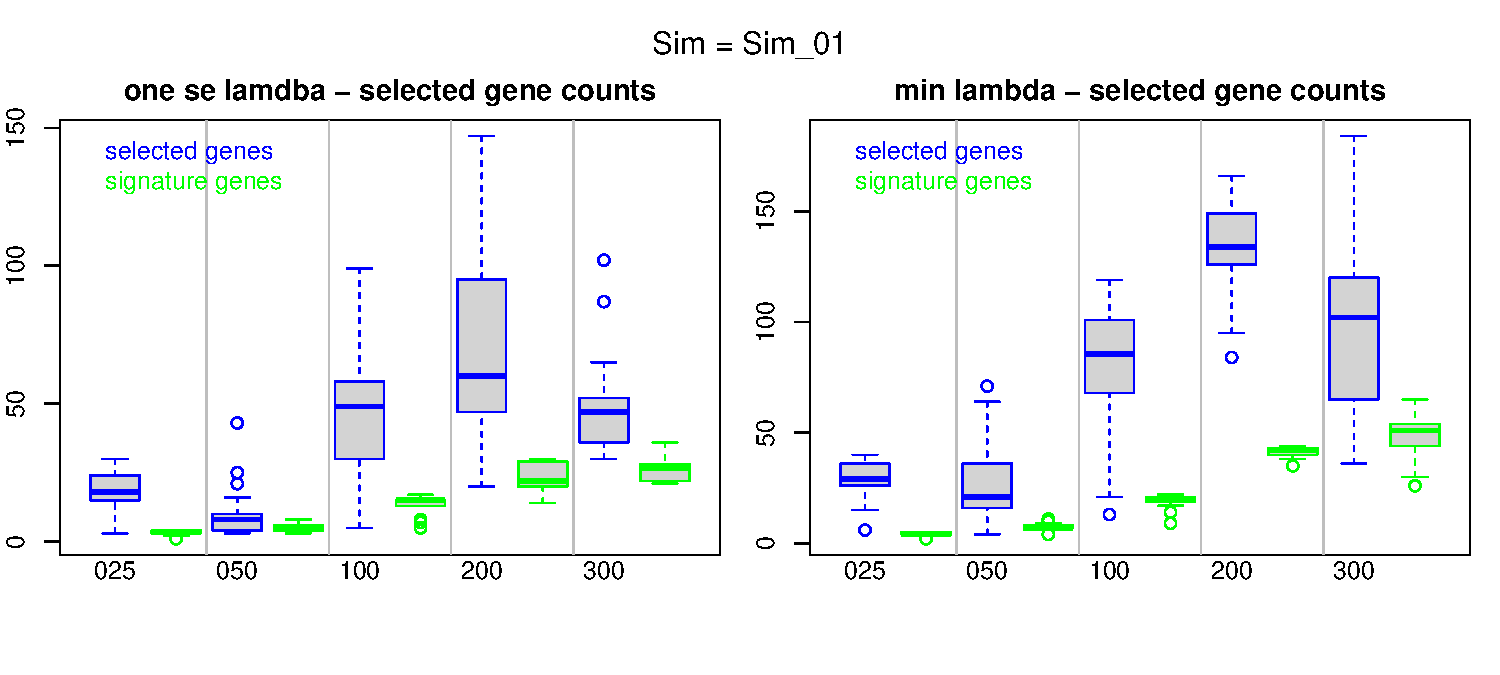
\includegraphics{Static/figures/enet-simRes-features-bySim-1.pdf}
\caption{\label{fig:enet-simRes-features-bySim}enet Models Selected Features by Sample Size}
\end{figure}

\hypertarget{summarize-results-across-simulation-runs}{%
\subsection*{Summarize results across simulation runs}\label{summarize-results-across-simulation-runs}}
\addcontentsline{toc}{subsection}{Summarize results across simulation runs}

\begin{Shaded}
\begin{Highlighting}[]
\CommentTok{\#\#\# CLEAR CACHE}

\CommentTok{\# get full model cv error ref}
\NormalTok{error\_1se\_vec <{-}}\StringTok{ }\KeywordTok{sapply}\NormalTok{(cv\_enetAll\_lst,}
 \ControlFlowTok{function}\NormalTok{(cv\_fit) cv\_fit}\OperatorTok{$}\NormalTok{cvm[cv\_fit}\OperatorTok{$}\NormalTok{lambda }\OperatorTok{==}\StringTok{ }\NormalTok{cv\_fit}\OperatorTok{$}\NormalTok{lambda}\FloatTok{.1}\NormalTok{se])}
\NormalTok{error\_1se\_q2 <{-}}\StringTok{ }\KeywordTok{quantile}\NormalTok{(error\_1se\_vec, }\DataTypeTok{prob=}\DecValTok{1}\OperatorTok{/}\DecValTok{2}\NormalTok{)        }

\NormalTok{error\_min\_vec <{-}}\StringTok{ }\KeywordTok{sapply}\NormalTok{(cv\_enetAll\_lst,}
 \ControlFlowTok{function}\NormalTok{(cv\_fit) cv\_fit}\OperatorTok{$}\NormalTok{cvm[cv\_fit}\OperatorTok{$}\NormalTok{lambda }\OperatorTok{==}\StringTok{ }\NormalTok{cv\_fit}\OperatorTok{$}\NormalTok{lambda.min])}
\NormalTok{error\_min\_q2 <{-}}\StringTok{ }\KeywordTok{quantile}\NormalTok{(error\_min\_vec, }\DataTypeTok{prob=}\DecValTok{1}\OperatorTok{/}\DecValTok{2}\NormalTok{)        }

\CommentTok{\# Utility objects}
\NormalTok{SIZE0 <{-}}\StringTok{ }\NormalTok{stringr}\OperatorTok{::}\KeywordTok{str\_pad}\NormalTok{(SIZE, }\DataTypeTok{width=}\DecValTok{3}\NormalTok{, }\DataTypeTok{pad=}\StringTok{\textquotesingle{}0\textquotesingle{}}\NormalTok{)}
\NormalTok{stage\_vec <{-}}\StringTok{ }\KeywordTok{cut}\NormalTok{(}\DecValTok{1}\OperatorTok{:}\KeywordTok{nrow}\NormalTok{(sim\_control\_qual\_mtx), }\KeywordTok{c}\NormalTok{(}\DecValTok{0}\NormalTok{,SIZE), }\DataTypeTok{include.lowest =}\NormalTok{ T)}

\KeywordTok{par}\NormalTok{(}\DataTypeTok{mfrow=}\KeywordTok{c}\NormalTok{(}\DecValTok{1}\NormalTok{,}\DecValTok{2}\NormalTok{), }\DataTypeTok{mar=}\KeywordTok{c}\NormalTok{(}\DecValTok{4}\NormalTok{, }\DecValTok{2}\NormalTok{, }\DecValTok{2}\NormalTok{, }\DecValTok{1}\NormalTok{), }\DataTypeTok{oma=}\KeywordTok{c}\NormalTok{(}\DecValTok{0}\NormalTok{,}\DecValTok{0}\NormalTok{,}\DecValTok{2}\NormalTok{,}\DecValTok{0}\NormalTok{))}
\CommentTok{\# 1se}
\CommentTok{\#\#\#\#\#\#\#\#\#\#\#\#\#\#\#\#\#\#\#\#\#\#\#\#\#\#\#\#\#\#\#\#\#\#\#\#\#\#\#\#\#}
\CommentTok{\#\# cv}
\NormalTok{cv\_1se\_Bysize\_lst <{-}}\StringTok{ }\KeywordTok{lapply}\NormalTok{(}\KeywordTok{unique}\NormalTok{(enet\_sim\_results\_frm}\OperatorTok{$}\NormalTok{Size),}
\ControlFlowTok{function}\NormalTok{(SizeVal) \{}
\NormalTok{ sizeVal\_results\_frm <{-}}\StringTok{ }\NormalTok{enet\_sim\_results\_frm }\OperatorTok{\%>\%}\StringTok{ }\NormalTok{dplyr}\OperatorTok{::}\KeywordTok{filter}\NormalTok{(Size}\OperatorTok{==}\NormalTok{SizeVal)}
\NormalTok{ sizeVal\_cv\_1se\_lst <{-}}\StringTok{ }\KeywordTok{with}\NormalTok{(sizeVal\_results\_frm, }\KeywordTok{split}\NormalTok{(cv\_1se, SimNo))}
 \KeywordTok{sapply}\NormalTok{(sizeVal\_cv\_1se\_lst, median)}
\NormalTok{\})}
\KeywordTok{names}\NormalTok{(cv\_1se\_Bysize\_lst) <{-}}\StringTok{ }\KeywordTok{paste0}\NormalTok{(}
\NormalTok{ stringr}\OperatorTok{::}\KeywordTok{str\_pad}\NormalTok{(}\KeywordTok{unique}\NormalTok{(enet\_sim\_results\_frm}\OperatorTok{$}\NormalTok{Size), }\DataTypeTok{width=}\DecValTok{3}\NormalTok{, }\DataTypeTok{pad=}\StringTok{\textquotesingle{}0\textquotesingle{}}\NormalTok{), }\StringTok{\textquotesingle{}\_cv\textquotesingle{}}\NormalTok{)}

\CommentTok{\#\# test}
\NormalTok{test\_1se\_Bysize\_lst <{-}}\StringTok{ }\KeywordTok{lapply}\NormalTok{(}\KeywordTok{unique}\NormalTok{(enet\_sim\_results\_frm}\OperatorTok{$}\NormalTok{Size),}
\ControlFlowTok{function}\NormalTok{(SizeVal) \{}
\NormalTok{ sizeVal\_results\_frm <{-}}\StringTok{ }\NormalTok{enet\_sim\_results\_frm }\OperatorTok{\%>\%}\StringTok{ }\NormalTok{dplyr}\OperatorTok{::}\KeywordTok{filter}\NormalTok{(Size}\OperatorTok{==}\NormalTok{SizeVal)}
\NormalTok{ sizeVal\_test\_1se\_lst <{-}}\StringTok{ }\KeywordTok{with}\NormalTok{(sizeVal\_results\_frm, }\KeywordTok{split}\NormalTok{(test\_1se, SimNo))}
 \KeywordTok{sapply}\NormalTok{(sizeVal\_test\_1se\_lst, median)}
\NormalTok{\})}
\KeywordTok{names}\NormalTok{(test\_1se\_Bysize\_lst) <{-}}\StringTok{ }\KeywordTok{paste0}\NormalTok{(}
\NormalTok{ stringr}\OperatorTok{::}\KeywordTok{str\_pad}\NormalTok{(}\KeywordTok{unique}\NormalTok{(enet\_sim\_results\_frm}\OperatorTok{$}\NormalTok{Size), }\DataTypeTok{width=}\DecValTok{3}\NormalTok{, }\DataTypeTok{pad=}\StringTok{\textquotesingle{}0\textquotesingle{}}\NormalTok{), }\StringTok{\textquotesingle{}\_test\textquotesingle{}}\NormalTok{)}


\NormalTok{error\_1se\_Bysize\_lst <{-}}\StringTok{ }\KeywordTok{c}\NormalTok{(cv\_1se\_Bysize\_lst, test\_1se\_Bysize\_lst)}
\NormalTok{error\_1se\_Bysize\_lst <{-}}\StringTok{ }\NormalTok{error\_1se\_Bysize\_lst[}\KeywordTok{order}\NormalTok{(}\KeywordTok{names}\NormalTok{(error\_1se\_Bysize\_lst))]}

\KeywordTok{boxplot}\NormalTok{(error\_1se\_Bysize\_lst,}
  \DataTypeTok{col=}\DecValTok{0}\NormalTok{,}
  \DataTypeTok{border=}\KeywordTok{c}\NormalTok{(}\StringTok{\textquotesingle{}blue\textquotesingle{}}\NormalTok{,}\StringTok{\textquotesingle{}green\textquotesingle{}}\NormalTok{),}
  \DataTypeTok{ylim=}\KeywordTok{c}\NormalTok{(}\FloatTok{0.05}\NormalTok{, }\FloatTok{.5}\NormalTok{),}
  \DataTypeTok{outline=}\NormalTok{F,}
  \DataTypeTok{xaxt=}\StringTok{\textquotesingle{}n\textquotesingle{}}
\NormalTok{)}
\ControlFlowTok{for}\NormalTok{(JJ }\ControlFlowTok{in} \DecValTok{1}\OperatorTok{:}\KeywordTok{length}\NormalTok{(error\_1se\_Bysize\_lst))}
\KeywordTok{points}\NormalTok{(}
   \DataTypeTok{x=}\KeywordTok{jitter}\NormalTok{(}\KeywordTok{rep}\NormalTok{(JJ, }\KeywordTok{length}\NormalTok{(error\_1se\_Bysize\_lst[[JJ]])), }\DataTypeTok{amount=}\FloatTok{0.25}\NormalTok{), }
   \DataTypeTok{y=}\NormalTok{error\_1se\_Bysize\_lst[[JJ]],}
   \DataTypeTok{col=}\KeywordTok{ifelse}\NormalTok{(}\KeywordTok{grepl}\NormalTok{(}\StringTok{\textquotesingle{}cv\textquotesingle{}}\NormalTok{, }\KeywordTok{names}\NormalTok{(error\_1se\_Bysize\_lst)[JJ]),}\StringTok{\textquotesingle{}blue\textquotesingle{}}\NormalTok{, }\StringTok{\textquotesingle{}green\textquotesingle{}}\NormalTok{)}
\NormalTok{)}
\NormalTok{LL <{-}}\StringTok{ }\DecValTok{{-}1}
\KeywordTok{axis}\NormalTok{(}\DataTypeTok{side=}\DecValTok{1}\NormalTok{, }\DataTypeTok{tick=}\NormalTok{F, }\DataTypeTok{line =}\NormalTok{ LL,}
  \DataTypeTok{at =} \KeywordTok{match}\NormalTok{(}\KeywordTok{paste0}\NormalTok{(SIZE0,}\StringTok{\textquotesingle{}\_cv\textquotesingle{}}\NormalTok{),}\KeywordTok{names}\NormalTok{(error\_1se\_Bysize\_lst)),}
\NormalTok{  SIZE0}
\NormalTok{ )}
\KeywordTok{abline}\NormalTok{(}\DataTypeTok{v=} \KeywordTok{match}\NormalTok{(}\KeywordTok{paste0}\NormalTok{(SIZE0,}\StringTok{\textquotesingle{}\_cv\textquotesingle{}}\NormalTok{),}\KeywordTok{names}\NormalTok{(error\_1se\_Bysize\_lst))[}\OperatorTok{{-}}\DecValTok{1}\NormalTok{] }\OperatorTok{{-}}\StringTok{ }\FloatTok{0.5}\NormalTok{, }\DataTypeTok{col=}\StringTok{\textquotesingle{}grey\textquotesingle{}}\NormalTok{)}
\KeywordTok{abline}\NormalTok{(}\DataTypeTok{h=}\NormalTok{ error\_min\_q2, }\DataTypeTok{col =} \StringTok{\textquotesingle{}red\textquotesingle{}}\NormalTok{)}
\KeywordTok{legend}\NormalTok{(}\StringTok{\textquotesingle{}topright\textquotesingle{}}\NormalTok{,}
   \CommentTok{\#title=\textquotesingle{}min errors\textquotesingle{}, title.col = \textquotesingle{}black\textquotesingle{},}
   \DataTypeTok{text.col =} \KeywordTok{c}\NormalTok{(}\StringTok{\textquotesingle{}blue\textquotesingle{}}\NormalTok{,}\StringTok{\textquotesingle{}green\textquotesingle{}}\NormalTok{),}
   \DataTypeTok{legend =} \KeywordTok{c}\NormalTok{(}\StringTok{\textquotesingle{}cv error\textquotesingle{}}\NormalTok{, }\StringTok{\textquotesingle{}test set\textquotesingle{}}\NormalTok{),}
   \DataTypeTok{bty=}\StringTok{\textquotesingle{}n\textquotesingle{}}
\NormalTok{ )}
\KeywordTok{title}\NormalTok{(}\KeywordTok{paste}\NormalTok{(}\StringTok{\textquotesingle{}one se lambda {-} error rates\textquotesingle{}}\NormalTok{))}


\CommentTok{\# min}
\CommentTok{\#\#\#\#\#\#\#\#\#\#\#\#\#\#\#\#\#\#\#\#\#\#\#\#\#\#\#\#\#\#\#\#\#\#\#\#\#\#\#\#\#}
\CommentTok{\#\# cv}
\NormalTok{cv\_min\_Bysize\_lst <{-}}\StringTok{ }\KeywordTok{lapply}\NormalTok{(}\KeywordTok{unique}\NormalTok{(enet\_sim\_results\_frm}\OperatorTok{$}\NormalTok{Size),}
\ControlFlowTok{function}\NormalTok{(SizeVal) \{}
\NormalTok{ sizeVal\_results\_frm <{-}}\StringTok{ }\NormalTok{enet\_sim\_results\_frm }\OperatorTok{\%>\%}\StringTok{ }\NormalTok{dplyr}\OperatorTok{::}\KeywordTok{filter}\NormalTok{(Size}\OperatorTok{==}\NormalTok{SizeVal)}
\NormalTok{ sizeVal\_cv\_min\_lst <{-}}\StringTok{ }\KeywordTok{with}\NormalTok{(sizeVal\_results\_frm, }\KeywordTok{split}\NormalTok{(cv\_min, SimNo))}
 \KeywordTok{sapply}\NormalTok{(sizeVal\_cv\_min\_lst, median)}
\NormalTok{\})}
\KeywordTok{names}\NormalTok{(cv\_min\_Bysize\_lst) <{-}}\StringTok{ }\KeywordTok{paste0}\NormalTok{(}
\NormalTok{ stringr}\OperatorTok{::}\KeywordTok{str\_pad}\NormalTok{(}\KeywordTok{unique}\NormalTok{(enet\_sim\_results\_frm}\OperatorTok{$}\NormalTok{Size), }\DataTypeTok{width=}\DecValTok{3}\NormalTok{, }\DataTypeTok{pad=}\StringTok{\textquotesingle{}0\textquotesingle{}}\NormalTok{), }\StringTok{\textquotesingle{}\_cv\textquotesingle{}}\NormalTok{)}

\CommentTok{\#\# test}
\NormalTok{test\_min\_Bysize\_lst <{-}}\StringTok{ }\KeywordTok{lapply}\NormalTok{(}\KeywordTok{unique}\NormalTok{(enet\_sim\_results\_frm}\OperatorTok{$}\NormalTok{Size),}
\ControlFlowTok{function}\NormalTok{(SizeVal) \{}
\NormalTok{ sizeVal\_results\_frm <{-}}\StringTok{ }\NormalTok{enet\_sim\_results\_frm }\OperatorTok{\%>\%}\StringTok{ }\NormalTok{dplyr}\OperatorTok{::}\KeywordTok{filter}\NormalTok{(Size}\OperatorTok{==}\NormalTok{SizeVal)}
\NormalTok{ sizeVal\_test\_min\_lst <{-}}\StringTok{ }\KeywordTok{with}\NormalTok{(sizeVal\_results\_frm, }\KeywordTok{split}\NormalTok{(test\_min, SimNo))}
 \KeywordTok{sapply}\NormalTok{(sizeVal\_test\_min\_lst, median)}
\NormalTok{\})}
\KeywordTok{names}\NormalTok{(test\_min\_Bysize\_lst) <{-}}\StringTok{ }\KeywordTok{paste0}\NormalTok{(}
\NormalTok{ stringr}\OperatorTok{::}\KeywordTok{str\_pad}\NormalTok{(}\KeywordTok{unique}\NormalTok{(enet\_sim\_results\_frm}\OperatorTok{$}\NormalTok{Size), }\DataTypeTok{width=}\DecValTok{3}\NormalTok{, }\DataTypeTok{pad=}\StringTok{\textquotesingle{}0\textquotesingle{}}\NormalTok{), }\StringTok{\textquotesingle{}\_test\textquotesingle{}}\NormalTok{)}


\NormalTok{error\_min\_Bysize\_lst <{-}}\StringTok{ }\KeywordTok{c}\NormalTok{(cv\_min\_Bysize\_lst, test\_min\_Bysize\_lst)}
\NormalTok{error\_min\_Bysize\_lst <{-}}\StringTok{ }\NormalTok{error\_min\_Bysize\_lst[}\KeywordTok{order}\NormalTok{(}\KeywordTok{names}\NormalTok{(error\_min\_Bysize\_lst))]}

\KeywordTok{boxplot}\NormalTok{(error\_min\_Bysize\_lst,}
  \DataTypeTok{col=}\DecValTok{0}\NormalTok{,}
  \DataTypeTok{border=}\KeywordTok{c}\NormalTok{(}\StringTok{\textquotesingle{}blue\textquotesingle{}}\NormalTok{,}\StringTok{\textquotesingle{}green\textquotesingle{}}\NormalTok{),}
  \DataTypeTok{ylim=}\KeywordTok{c}\NormalTok{(}\FloatTok{0.05}\NormalTok{, }\FloatTok{.5}\NormalTok{),}
  \DataTypeTok{outline=}\NormalTok{F,}
  \DataTypeTok{xaxt=}\StringTok{\textquotesingle{}n\textquotesingle{}}
\NormalTok{)}
\ControlFlowTok{for}\NormalTok{(JJ }\ControlFlowTok{in} \DecValTok{1}\OperatorTok{:}\KeywordTok{length}\NormalTok{(error\_min\_Bysize\_lst))}
\KeywordTok{points}\NormalTok{(}
   \DataTypeTok{x=}\KeywordTok{jitter}\NormalTok{(}\KeywordTok{rep}\NormalTok{(JJ, }\KeywordTok{length}\NormalTok{(error\_min\_Bysize\_lst[[JJ]])), }\DataTypeTok{amount=}\FloatTok{0.25}\NormalTok{), }
   \DataTypeTok{y=}\NormalTok{error\_min\_Bysize\_lst[[JJ]],}
   \DataTypeTok{col=}\KeywordTok{ifelse}\NormalTok{(}\KeywordTok{grepl}\NormalTok{(}\StringTok{\textquotesingle{}cv\textquotesingle{}}\NormalTok{, }\KeywordTok{names}\NormalTok{(error\_min\_Bysize\_lst)[JJ]),}\StringTok{\textquotesingle{}blue\textquotesingle{}}\NormalTok{, }\StringTok{\textquotesingle{}green\textquotesingle{}}\NormalTok{)}
\NormalTok{)}
\NormalTok{LL <{-}}\StringTok{ }\DecValTok{{-}1}
\KeywordTok{axis}\NormalTok{(}\DataTypeTok{side=}\DecValTok{1}\NormalTok{, }\DataTypeTok{tick=}\NormalTok{F, }\DataTypeTok{line =}\NormalTok{ LL,}
  \DataTypeTok{at =} \KeywordTok{match}\NormalTok{(}\KeywordTok{paste0}\NormalTok{(SIZE0,}\StringTok{\textquotesingle{}\_cv\textquotesingle{}}\NormalTok{),}\KeywordTok{names}\NormalTok{(error\_min\_Bysize\_lst)),}
\NormalTok{  SIZE0}
\NormalTok{ )}
\KeywordTok{abline}\NormalTok{(}\DataTypeTok{v=} \KeywordTok{match}\NormalTok{(}\KeywordTok{paste0}\NormalTok{(SIZE0,}\StringTok{\textquotesingle{}\_cv\textquotesingle{}}\NormalTok{),}\KeywordTok{names}\NormalTok{(error\_min\_Bysize\_lst))[}\OperatorTok{{-}}\DecValTok{1}\NormalTok{] }\OperatorTok{{-}}\StringTok{ }\FloatTok{0.5}\NormalTok{, }\DataTypeTok{col=}\StringTok{\textquotesingle{}grey\textquotesingle{}}\NormalTok{)}
\KeywordTok{abline}\NormalTok{(}\DataTypeTok{h=}\NormalTok{ error\_min\_q2, }\DataTypeTok{col =} \StringTok{\textquotesingle{}red\textquotesingle{}}\NormalTok{)}
\KeywordTok{legend}\NormalTok{(}\StringTok{\textquotesingle{}topright\textquotesingle{}}\NormalTok{,}
   \CommentTok{\#title=\textquotesingle{}min errors\textquotesingle{}, title.col = \textquotesingle{}black\textquotesingle{},}
   \DataTypeTok{text.col =} \KeywordTok{c}\NormalTok{(}\StringTok{\textquotesingle{}blue\textquotesingle{}}\NormalTok{,}\StringTok{\textquotesingle{}green\textquotesingle{}}\NormalTok{),}
   \DataTypeTok{legend =} \KeywordTok{c}\NormalTok{(}\StringTok{\textquotesingle{}cv error\textquotesingle{}}\NormalTok{, }\StringTok{\textquotesingle{}test set\textquotesingle{}}\NormalTok{),}
   \DataTypeTok{bty=}\StringTok{\textquotesingle{}n\textquotesingle{}}
\NormalTok{ )}
\KeywordTok{title}\NormalTok{(}\KeywordTok{paste}\NormalTok{(}\StringTok{\textquotesingle{}min lambda {-} error rates\textquotesingle{}}\NormalTok{))}


\KeywordTok{mtext}\NormalTok{(}\DataTypeTok{side=}\DecValTok{3}\NormalTok{, }\DataTypeTok{outer=}\NormalTok{T, }\DataTypeTok{cex=}\FloatTok{1.25}\NormalTok{, }\KeywordTok{paste}\NormalTok{(}\StringTok{\textquotesingle{}enet fit error rates summarized across simulations\textquotesingle{}}\NormalTok{))}
\end{Highlighting}
\end{Shaded}

\begin{figure}
\centering
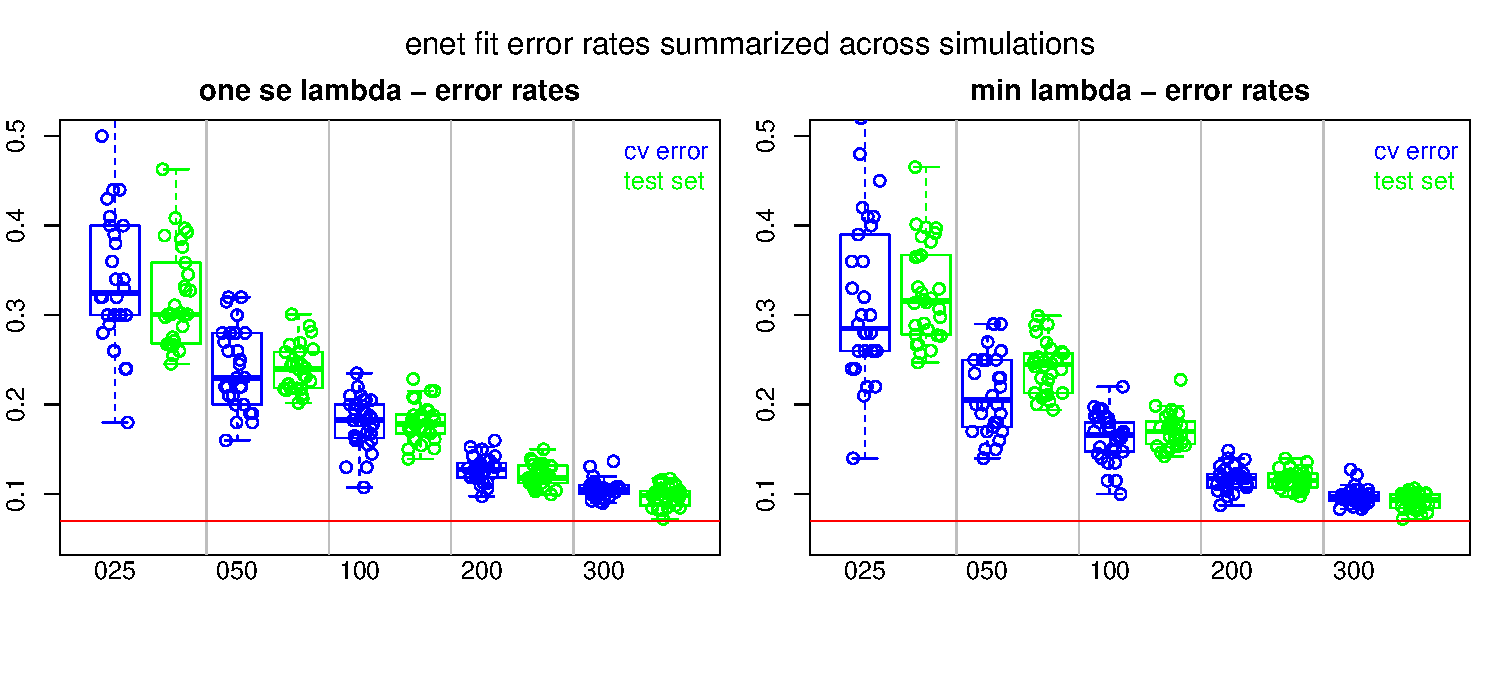
\includegraphics{Static/figures/enet-simRes-errors-overSim-1.pdf}
\caption{\label{fig:enet-simRes-errors-overSim}enet Model Errors by Sample Size}
\end{figure}

\begin{Shaded}
\begin{Highlighting}[]
\CommentTok{\#\#\# CLEAR CACHE}

\NormalTok{error\_1se\_Bysize\_sum\_frm <{-}}\StringTok{ }\KeywordTok{t}\NormalTok{(}\KeywordTok{sapply}\NormalTok{(error\_1se\_Bysize\_lst, }\ControlFlowTok{function}\NormalTok{(LL) }\KeywordTok{quantile}\NormalTok{(LL, }\DataTypeTok{prob=}\NormalTok{(}\DecValTok{1}\OperatorTok{:}\DecValTok{3}\NormalTok{)}\OperatorTok{/}\DecValTok{4}\NormalTok{)))}
\KeywordTok{colnames}\NormalTok{(error\_1se\_Bysize\_sum\_frm) <{-}}\StringTok{ }\KeywordTok{paste0}\NormalTok{(}\StringTok{\textquotesingle{}1se\_\textquotesingle{}}\NormalTok{, }\KeywordTok{colnames}\NormalTok{(error\_1se\_Bysize\_sum\_frm))}


\NormalTok{error\_min\_Bysize\_sum\_frm <{-}}\StringTok{ }\KeywordTok{t}\NormalTok{(}\KeywordTok{sapply}\NormalTok{(error\_min\_Bysize\_lst, }\ControlFlowTok{function}\NormalTok{(LL) }\KeywordTok{quantile}\NormalTok{(LL, }\DataTypeTok{prob=}\NormalTok{(}\DecValTok{1}\OperatorTok{:}\DecValTok{3}\NormalTok{)}\OperatorTok{/}\DecValTok{4}\NormalTok{)))}
\KeywordTok{colnames}\NormalTok{(error\_min\_Bysize\_sum\_frm) <{-}}\StringTok{ }\KeywordTok{paste0}\NormalTok{(}\StringTok{\textquotesingle{}min\_\textquotesingle{}}\NormalTok{, }\KeywordTok{colnames}\NormalTok{(error\_min\_Bysize\_sum\_frm))}


\NormalTok{knitr}\OperatorTok{::}\KeywordTok{kable}\NormalTok{(}\KeywordTok{cbind}\NormalTok{(}\StringTok{\textasciigrave{}}\DataTypeTok{1se}\StringTok{\textasciigrave{}}\NormalTok{=error\_1se\_Bysize\_sum\_frm, }\DataTypeTok{min=}\NormalTok{error\_min\_Bysize\_sum\_frm),}
      \DataTypeTok{caption =} \KeywordTok{paste}\NormalTok{(}\StringTok{"elastic net error rates by sample size across simulations"}\NormalTok{),}
    \DataTypeTok{digits=}\DecValTok{2}\NormalTok{) }\OperatorTok{\%>\%}
\StringTok{   }\NormalTok{kableExtra}\OperatorTok{::}\KeywordTok{kable\_styling}\NormalTok{(}\DataTypeTok{full\_width =}\NormalTok{ F)}
\end{Highlighting}
\end{Shaded}

\begin{table}

\caption{\label{tab:print-enet-simRes-errors-overSim}elastic net error rates by sample size across simulations}
\centering
\begin{tabular}[t]{l|r|r|r|r|r|r}
\hline
  & 1se\_25\% & 1se\_50\% & 1se\_75\% & min\_25\% & min\_50\% & min\_75\%\\
\hline
025\_cv & 0.30 & 0.32 & 0.40 & 0.26 & 0.29 & 0.38\\
\hline
025\_test & 0.27 & 0.30 & 0.36 & 0.28 & 0.32 & 0.37\\
\hline
050\_cv & 0.20 & 0.23 & 0.28 & 0.18 & 0.21 & 0.25\\
\hline
050\_test & 0.22 & 0.24 & 0.26 & 0.21 & 0.24 & 0.26\\
\hline
100\_cv & 0.16 & 0.18 & 0.20 & 0.15 & 0.17 & 0.18\\
\hline
100\_test & 0.17 & 0.18 & 0.19 & 0.16 & 0.17 & 0.18\\
\hline
200\_cv & 0.12 & 0.13 & 0.13 & 0.11 & 0.12 & 0.12\\
\hline
200\_test & 0.11 & 0.12 & 0.13 & 0.11 & 0.12 & 0.12\\
\hline
300\_cv & 0.10 & 0.10 & 0.11 & 0.09 & 0.10 & 0.10\\
\hline
300\_test & 0.09 & 0.10 & 0.10 & 0.08 & 0.09 & 0.10\\
\hline
\end{tabular}
\end{table}

Now look at feature selection.

\begin{Shaded}
\begin{Highlighting}[]
\CommentTok{\#\#\# CLEAR CACHE}

\CommentTok{\# Utility objects}
\NormalTok{SIZE0 <{-}}\StringTok{ }\NormalTok{stringr}\OperatorTok{::}\KeywordTok{str\_pad}\NormalTok{(SIZE, }\DataTypeTok{width=}\DecValTok{3}\NormalTok{, }\DataTypeTok{pad=}\StringTok{\textquotesingle{}0\textquotesingle{}}\NormalTok{)}
\NormalTok{stage\_vec <{-}}\StringTok{ }\KeywordTok{cut}\NormalTok{(}\DecValTok{1}\OperatorTok{:}\KeywordTok{nrow}\NormalTok{(sim\_control\_qual\_mtx), }\KeywordTok{c}\NormalTok{(}\DecValTok{0}\NormalTok{,SIZE), }\DataTypeTok{include.lowest =}\NormalTok{ T)}

\KeywordTok{par}\NormalTok{(}\DataTypeTok{mfrow=}\KeywordTok{c}\NormalTok{(}\DecValTok{1}\NormalTok{,}\DecValTok{2}\NormalTok{), }\DataTypeTok{mar=}\KeywordTok{c}\NormalTok{(}\DecValTok{4}\NormalTok{, }\DecValTok{2}\NormalTok{, }\DecValTok{2}\NormalTok{, }\DecValTok{1}\NormalTok{), }\DataTypeTok{oma=}\KeywordTok{c}\NormalTok{(}\DecValTok{0}\NormalTok{,}\DecValTok{0}\NormalTok{,}\DecValTok{2}\NormalTok{,}\DecValTok{0}\NormalTok{))}
\CommentTok{\# 1se}
\CommentTok{\#\#\#\#\#\#\#\#\#\#\#\#\#\#\#\#\#\#\#\#\#\#\#\#\#\#\#\#\#\#\#\#\#\#\#\#\#\#\#\#\#}
\CommentTok{\# selected features}
\NormalTok{p\_1se\_Bysize\_lst <{-}}\StringTok{ }\KeywordTok{lapply}\NormalTok{(}\KeywordTok{unique}\NormalTok{(enet\_sim\_results\_frm}\OperatorTok{$}\NormalTok{Size),}
\ControlFlowTok{function}\NormalTok{(SizeVal) \{}
\NormalTok{ sizeVal\_results\_frm <{-}}\StringTok{ }\NormalTok{enet\_sim\_results\_frm }\OperatorTok{\%>\%}\StringTok{ }\NormalTok{dplyr}\OperatorTok{::}\KeywordTok{filter}\NormalTok{(Size}\OperatorTok{==}\NormalTok{SizeVal)}
\NormalTok{ sizeVal\_p\_1se\_lst <{-}}\StringTok{ }\KeywordTok{with}\NormalTok{(sizeVal\_results\_frm, }\KeywordTok{split}\NormalTok{(p\_1se, SimNo))}
 \KeywordTok{sapply}\NormalTok{(sizeVal\_p\_1se\_lst, median)}
\NormalTok{\})}
\KeywordTok{names}\NormalTok{(p\_1se\_Bysize\_lst) <{-}}\StringTok{ }\KeywordTok{paste0}\NormalTok{(}
\NormalTok{ stringr}\OperatorTok{::}\KeywordTok{str\_pad}\NormalTok{(}\KeywordTok{unique}\NormalTok{(enet\_sim\_results\_frm}\OperatorTok{$}\NormalTok{Size), }\DataTypeTok{width=}\DecValTok{3}\NormalTok{, }\DataTypeTok{pad=}\StringTok{\textquotesingle{}0\textquotesingle{}}\NormalTok{), }\StringTok{\textquotesingle{}\_p\textquotesingle{}}\NormalTok{)}

\CommentTok{\# selected signatue features}
\NormalTok{sign\_p\_1se\_Bysize\_lst <{-}}\StringTok{ }\KeywordTok{lapply}\NormalTok{(}\KeywordTok{unique}\NormalTok{(enet\_sim\_results\_frm}\OperatorTok{$}\NormalTok{Size),}
\ControlFlowTok{function}\NormalTok{(SizeVal) \{}
\NormalTok{ sizeVal\_results\_frm <{-}}\StringTok{ }\NormalTok{enet\_sim\_results\_frm }\OperatorTok{\%>\%}\StringTok{ }\NormalTok{dplyr}\OperatorTok{::}\KeywordTok{filter}\NormalTok{(Size}\OperatorTok{==}\NormalTok{SizeVal)}
 
  
\NormalTok{ sizeVal\_sign\_genes\_1se\_lst <{-}}\StringTok{ }\KeywordTok{lapply}\NormalTok{(}\DecValTok{1}\OperatorTok{:}\KeywordTok{nrow}\NormalTok{(sizeVal\_results\_frm), }\ControlFlowTok{function}\NormalTok{(RR)}
    \KeywordTok{intersect}\NormalTok{(}\KeywordTok{unlist}\NormalTok{(sizeVal\_results\_frm[RR, }\StringTok{\textquotesingle{}genes\_1se\textquotesingle{}}\NormalTok{]), enet\_gene\_sign\_1se\_vec))}

\NormalTok{ sizeVal\_sign\_p\_1se\_lst <{-}}\StringTok{ }\KeywordTok{split}\NormalTok{(}\KeywordTok{sapply}\NormalTok{(sizeVal\_sign\_genes\_1se\_lst, length),}
\NormalTok{    sizeVal\_results\_frm}\OperatorTok{$}\NormalTok{SimNo)}
 
 \KeywordTok{sapply}\NormalTok{(sizeVal\_sign\_p\_1se\_lst, median)}
\NormalTok{\})}
\KeywordTok{names}\NormalTok{(sign\_p\_1se\_Bysize\_lst) <{-}}\StringTok{ }\KeywordTok{paste0}\NormalTok{(}
\NormalTok{ stringr}\OperatorTok{::}\KeywordTok{str\_pad}\NormalTok{(}\KeywordTok{unique}\NormalTok{(enet\_sim\_results\_frm}\OperatorTok{$}\NormalTok{Size), }\DataTypeTok{width=}\DecValTok{3}\NormalTok{, }\DataTypeTok{pad=}\StringTok{\textquotesingle{}0\textquotesingle{}}\NormalTok{), }\StringTok{\textquotesingle{}\_signP\textquotesingle{}}\NormalTok{)}


\NormalTok{p\_singP\_1se\_Bysize\_lst <{-}}\StringTok{ }\KeywordTok{c}\NormalTok{(p\_1se\_Bysize\_lst, sign\_p\_1se\_Bysize\_lst)}
\NormalTok{p\_singP\_1se\_Bysize\_lst <{-}}\StringTok{ }\NormalTok{p\_singP\_1se\_Bysize\_lst[}\KeywordTok{order}\NormalTok{(}\KeywordTok{names}\NormalTok{(p\_singP\_1se\_Bysize\_lst))]}

\KeywordTok{boxplot}\NormalTok{(p\_singP\_1se\_Bysize\_lst,}
  \DataTypeTok{col=}\DecValTok{0}\NormalTok{,}
  \DataTypeTok{border=}\KeywordTok{c}\NormalTok{(}\StringTok{\textquotesingle{}blue\textquotesingle{}}\NormalTok{,}\StringTok{\textquotesingle{}green\textquotesingle{}}\NormalTok{),}
  \CommentTok{\#ylim=c(0, 300),}
  \DataTypeTok{xaxt=}\StringTok{\textquotesingle{}n\textquotesingle{}}
\NormalTok{)}
\ControlFlowTok{for}\NormalTok{(JJ }\ControlFlowTok{in} \DecValTok{1}\OperatorTok{:}\KeywordTok{length}\NormalTok{(p\_singP\_1se\_Bysize\_lst))}
\KeywordTok{points}\NormalTok{(}
   \DataTypeTok{x=}\KeywordTok{jitter}\NormalTok{(}\KeywordTok{rep}\NormalTok{(JJ, }\KeywordTok{length}\NormalTok{(p\_singP\_1se\_Bysize\_lst[[JJ]])), }\DataTypeTok{amount=}\FloatTok{0.25}\NormalTok{),}
   \DataTypeTok{y=}\NormalTok{p\_singP\_1se\_Bysize\_lst[[JJ]],}
   \DataTypeTok{col=}\KeywordTok{ifelse}\NormalTok{(}\KeywordTok{grepl}\NormalTok{(}\StringTok{\textquotesingle{}\_p\textquotesingle{}}\NormalTok{, }\KeywordTok{names}\NormalTok{(p\_singP\_1se\_Bysize\_lst)[JJ]),}\StringTok{\textquotesingle{}blue\textquotesingle{}}\NormalTok{, }\StringTok{\textquotesingle{}green\textquotesingle{}}\NormalTok{)}
\NormalTok{)}

\NormalTok{LL <{-}}\StringTok{ }\DecValTok{{-}1}
\KeywordTok{axis}\NormalTok{(}\DataTypeTok{side=}\DecValTok{1}\NormalTok{, }\DataTypeTok{tick=}\NormalTok{F, }\DataTypeTok{line =}\NormalTok{ LL,}
  \DataTypeTok{at =} \KeywordTok{match}\NormalTok{(}\KeywordTok{paste0}\NormalTok{(SIZE0,}\StringTok{\textquotesingle{}\_p\textquotesingle{}}\NormalTok{),}\KeywordTok{names}\NormalTok{(p\_singP\_1se\_Bysize\_lst)),}
\NormalTok{  SIZE0}
\NormalTok{ )}
\KeywordTok{abline}\NormalTok{(}\DataTypeTok{v=} \KeywordTok{match}\NormalTok{(}\KeywordTok{paste0}\NormalTok{(SIZE0,}\StringTok{\textquotesingle{}\_p\textquotesingle{}}\NormalTok{),}\KeywordTok{names}\NormalTok{(p\_singP\_1se\_Bysize\_lst))[}\OperatorTok{{-}}\DecValTok{1}\NormalTok{] }\OperatorTok{{-}}\StringTok{ }\FloatTok{0.5}\NormalTok{, }\DataTypeTok{col=}\StringTok{\textquotesingle{}grey\textquotesingle{}}\NormalTok{)}
\CommentTok{\#abline(h= nzero\_1se\_q2, col = \textquotesingle{}red\textquotesingle{})}
\KeywordTok{legend}\NormalTok{(}\StringTok{\textquotesingle{}topleft\textquotesingle{}}\NormalTok{,}
   \CommentTok{\#title=\textquotesingle{}1se errors\textquotesingle{}, title.col = \textquotesingle{}black\textquotesingle{},}
   \DataTypeTok{text.col =} \KeywordTok{c}\NormalTok{(}\StringTok{\textquotesingle{}blue\textquotesingle{}}\NormalTok{, }\StringTok{\textquotesingle{}green\textquotesingle{}}\NormalTok{),}
   \DataTypeTok{legend=} \KeywordTok{c}\NormalTok{(}\StringTok{\textquotesingle{}selected genes\textquotesingle{}}\NormalTok{,}\StringTok{\textquotesingle{}signature genes\textquotesingle{}}\NormalTok{),}
   \DataTypeTok{bty=}\StringTok{\textquotesingle{}n\textquotesingle{}}
\NormalTok{ )}
\KeywordTok{title}\NormalTok{(}\KeywordTok{paste}\NormalTok{(}\StringTok{\textquotesingle{}one se lamdba {-} selected gene counts\textquotesingle{}}\NormalTok{))}


\CommentTok{\# min}
\CommentTok{\#\#\#\#\#\#\#\#\#\#\#\#\#\#\#\#\#\#\#\#\#\#\#\#\#\#\#\#\#\#\#\#\#\#\#\#\#\#\#\#\#}
\CommentTok{\# selected features}
\NormalTok{p\_min\_Bysize\_lst <{-}}\StringTok{ }\KeywordTok{lapply}\NormalTok{(}\KeywordTok{unique}\NormalTok{(enet\_sim\_results\_frm}\OperatorTok{$}\NormalTok{Size),}
\ControlFlowTok{function}\NormalTok{(SizeVal) \{}
\NormalTok{ sizeVal\_results\_frm <{-}}\StringTok{ }\NormalTok{enet\_sim\_results\_frm }\OperatorTok{\%>\%}\StringTok{ }\NormalTok{dplyr}\OperatorTok{::}\KeywordTok{filter}\NormalTok{(Size}\OperatorTok{==}\NormalTok{SizeVal)}
\NormalTok{ sizeVal\_p\_min\_lst <{-}}\StringTok{ }\KeywordTok{with}\NormalTok{(sizeVal\_results\_frm, }\KeywordTok{split}\NormalTok{(p\_min, SimNo))}
 \KeywordTok{sapply}\NormalTok{(sizeVal\_p\_min\_lst, median)}
\NormalTok{\})}
\KeywordTok{names}\NormalTok{(p\_min\_Bysize\_lst) <{-}}\StringTok{ }\KeywordTok{paste0}\NormalTok{(}
\NormalTok{ stringr}\OperatorTok{::}\KeywordTok{str\_pad}\NormalTok{(}\KeywordTok{unique}\NormalTok{(enet\_sim\_results\_frm}\OperatorTok{$}\NormalTok{Size), }\DataTypeTok{width=}\DecValTok{3}\NormalTok{, }\DataTypeTok{pad=}\StringTok{\textquotesingle{}0\textquotesingle{}}\NormalTok{), }\StringTok{\textquotesingle{}\_p\textquotesingle{}}\NormalTok{)}

\CommentTok{\# selected signatue features}
\NormalTok{sign\_p\_min\_Bysize\_lst <{-}}\StringTok{ }\KeywordTok{lapply}\NormalTok{(}\KeywordTok{unique}\NormalTok{(enet\_sim\_results\_frm}\OperatorTok{$}\NormalTok{Size),}
\ControlFlowTok{function}\NormalTok{(SizeVal) \{}
\NormalTok{ sizeVal\_results\_frm <{-}}\StringTok{ }\NormalTok{enet\_sim\_results\_frm }\OperatorTok{\%>\%}\StringTok{ }\NormalTok{dplyr}\OperatorTok{::}\KeywordTok{filter}\NormalTok{(Size}\OperatorTok{==}\NormalTok{SizeVal)}
 
  
\NormalTok{ sizeVal\_sign\_genes\_min\_lst <{-}}\StringTok{ }\KeywordTok{lapply}\NormalTok{(}\DecValTok{1}\OperatorTok{:}\KeywordTok{nrow}\NormalTok{(sizeVal\_results\_frm), }\ControlFlowTok{function}\NormalTok{(RR)}
    \KeywordTok{intersect}\NormalTok{(}\KeywordTok{unlist}\NormalTok{(sizeVal\_results\_frm[RR, }\StringTok{\textquotesingle{}genes\_min\textquotesingle{}}\NormalTok{]), enet\_gene\_sign\_min\_vec))}

\NormalTok{ sizeVal\_sign\_p\_min\_lst <{-}}\StringTok{ }\KeywordTok{split}\NormalTok{(}\KeywordTok{sapply}\NormalTok{(sizeVal\_sign\_genes\_min\_lst, length),}
\NormalTok{    sizeVal\_results\_frm}\OperatorTok{$}\NormalTok{SimNo)}
 
 \KeywordTok{sapply}\NormalTok{(sizeVal\_sign\_p\_min\_lst, median)}
\NormalTok{\})}
\KeywordTok{names}\NormalTok{(sign\_p\_min\_Bysize\_lst) <{-}}\StringTok{ }\KeywordTok{paste0}\NormalTok{(}
\NormalTok{ stringr}\OperatorTok{::}\KeywordTok{str\_pad}\NormalTok{(}\KeywordTok{unique}\NormalTok{(enet\_sim\_results\_frm}\OperatorTok{$}\NormalTok{Size), }\DataTypeTok{width=}\DecValTok{3}\NormalTok{, }\DataTypeTok{pad=}\StringTok{\textquotesingle{}0\textquotesingle{}}\NormalTok{), }\StringTok{\textquotesingle{}\_signP\textquotesingle{}}\NormalTok{)}


\NormalTok{p\_singP\_min\_Bysize\_lst <{-}}\StringTok{ }\KeywordTok{c}\NormalTok{(p\_min\_Bysize\_lst, sign\_p\_min\_Bysize\_lst)}
\NormalTok{p\_singP\_min\_Bysize\_lst <{-}}\StringTok{ }\NormalTok{p\_singP\_min\_Bysize\_lst[}\KeywordTok{order}\NormalTok{(}\KeywordTok{names}\NormalTok{(p\_singP\_min\_Bysize\_lst))]}

\KeywordTok{boxplot}\NormalTok{(p\_singP\_min\_Bysize\_lst,}
  \DataTypeTok{col=}\DecValTok{0}\NormalTok{,}
  \DataTypeTok{border=}\KeywordTok{c}\NormalTok{(}\StringTok{\textquotesingle{}blue\textquotesingle{}}\NormalTok{,}\StringTok{\textquotesingle{}green\textquotesingle{}}\NormalTok{),}
  \CommentTok{\#ylim=c(0, 300),}
  \DataTypeTok{xaxt=}\StringTok{\textquotesingle{}n\textquotesingle{}}
\NormalTok{)}
\ControlFlowTok{for}\NormalTok{(JJ }\ControlFlowTok{in} \DecValTok{1}\OperatorTok{:}\KeywordTok{length}\NormalTok{(p\_singP\_min\_Bysize\_lst))}
\KeywordTok{points}\NormalTok{(}
   \DataTypeTok{x=}\KeywordTok{jitter}\NormalTok{(}\KeywordTok{rep}\NormalTok{(JJ, }\KeywordTok{length}\NormalTok{(p\_singP\_min\_Bysize\_lst[[JJ]])), }\DataTypeTok{amount=}\FloatTok{0.25}\NormalTok{),}
   \DataTypeTok{y=}\NormalTok{p\_singP\_min\_Bysize\_lst[[JJ]],}
   \DataTypeTok{col=}\KeywordTok{ifelse}\NormalTok{(}\KeywordTok{grepl}\NormalTok{(}\StringTok{\textquotesingle{}\_p\textquotesingle{}}\NormalTok{, }\KeywordTok{names}\NormalTok{(p\_singP\_min\_Bysize\_lst)[JJ]),}\StringTok{\textquotesingle{}blue\textquotesingle{}}\NormalTok{, }\StringTok{\textquotesingle{}green\textquotesingle{}}\NormalTok{)}
\NormalTok{)}

\NormalTok{LL <{-}}\StringTok{ }\DecValTok{{-}1}
\KeywordTok{axis}\NormalTok{(}\DataTypeTok{side=}\DecValTok{1}\NormalTok{, }\DataTypeTok{tick=}\NormalTok{F, }\DataTypeTok{line =}\NormalTok{ LL,}
  \DataTypeTok{at =} \KeywordTok{match}\NormalTok{(}\KeywordTok{paste0}\NormalTok{(SIZE0,}\StringTok{\textquotesingle{}\_p\textquotesingle{}}\NormalTok{),}\KeywordTok{names}\NormalTok{(p\_singP\_min\_Bysize\_lst)),}
\NormalTok{  SIZE0}
\NormalTok{ )}
\KeywordTok{abline}\NormalTok{(}\DataTypeTok{v=} \KeywordTok{match}\NormalTok{(}\KeywordTok{paste0}\NormalTok{(SIZE0,}\StringTok{\textquotesingle{}\_p\textquotesingle{}}\NormalTok{),}\KeywordTok{names}\NormalTok{(p\_singP\_min\_Bysize\_lst))[}\OperatorTok{{-}}\DecValTok{1}\NormalTok{] }\OperatorTok{{-}}\StringTok{ }\FloatTok{0.5}\NormalTok{, }\DataTypeTok{col=}\StringTok{\textquotesingle{}grey\textquotesingle{}}\NormalTok{)}
\CommentTok{\#abline(h= nzero\_min\_q2, col = \textquotesingle{}red\textquotesingle{})}
\KeywordTok{legend}\NormalTok{(}\StringTok{\textquotesingle{}topleft\textquotesingle{}}\NormalTok{,}
   \CommentTok{\#title=\textquotesingle{}min errors\textquotesingle{}, title.col = \textquotesingle{}black\textquotesingle{},}
   \DataTypeTok{text.col =} \KeywordTok{c}\NormalTok{(}\StringTok{\textquotesingle{}blue\textquotesingle{}}\NormalTok{, }\StringTok{\textquotesingle{}green\textquotesingle{}}\NormalTok{),}
   \DataTypeTok{legend=} \KeywordTok{c}\NormalTok{(}\StringTok{\textquotesingle{}selected genes\textquotesingle{}}\NormalTok{,}\StringTok{\textquotesingle{}signature genes\textquotesingle{}}\NormalTok{),}
   \DataTypeTok{bty=}\StringTok{\textquotesingle{}n\textquotesingle{}}
\NormalTok{ )}
\KeywordTok{title}\NormalTok{(}\KeywordTok{paste}\NormalTok{(}\StringTok{\textquotesingle{}min lambda {-} selected gene counts\textquotesingle{}}\NormalTok{))}

\KeywordTok{mtext}\NormalTok{(}\DataTypeTok{side=}\DecValTok{3}\NormalTok{, }\DataTypeTok{outer=}\NormalTok{T, }\DataTypeTok{cex=}\FloatTok{1.25}\NormalTok{, }\KeywordTok{paste}\NormalTok{(}\StringTok{\textquotesingle{}enet fit feature selection summarized across simulations\textquotesingle{}}\NormalTok{))}
\end{Highlighting}
\end{Shaded}

\begin{figure}
\centering
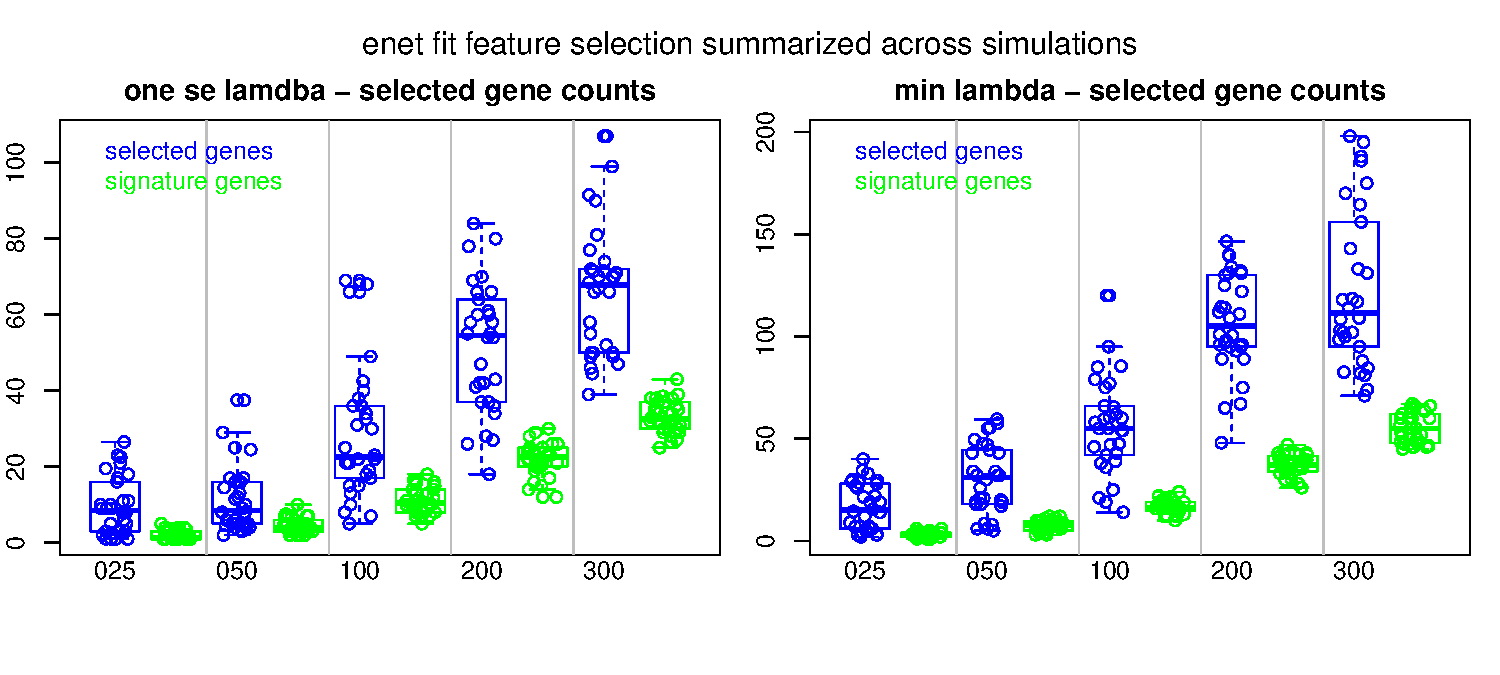
\includegraphics{Static/figures/enet-simRes-features-OverSim-1.pdf}
\caption{\label{fig:enet-simRes-features-OverSim}enet Models Selected Features by Sample Size}
\end{figure}

\begin{Shaded}
\begin{Highlighting}[]
\CommentTok{\#\#\# CLEAR CACHE}

\NormalTok{p\_sing\_1se\_Bysize\_sum\_frm <{-}}\StringTok{ }\KeywordTok{t}\NormalTok{(}\KeywordTok{sapply}\NormalTok{(p\_singP\_1se\_Bysize\_lst, }\ControlFlowTok{function}\NormalTok{(LL) }\KeywordTok{quantile}\NormalTok{(LL, }\DataTypeTok{prob=}\NormalTok{(}\DecValTok{1}\OperatorTok{:}\DecValTok{3}\NormalTok{)}\OperatorTok{/}\DecValTok{4}\NormalTok{)))}
\KeywordTok{colnames}\NormalTok{(p\_sing\_1se\_Bysize\_sum\_frm) <{-}}\StringTok{ }\KeywordTok{paste0}\NormalTok{(}\StringTok{\textquotesingle{}1se\_\textquotesingle{}}\NormalTok{, }\KeywordTok{colnames}\NormalTok{(p\_sing\_1se\_Bysize\_sum\_frm))}

\NormalTok{p\_sing\_min\_Bysize\_sum\_frm <{-}}\StringTok{ }\KeywordTok{t}\NormalTok{(}\KeywordTok{sapply}\NormalTok{(p\_singP\_min\_Bysize\_lst, }\ControlFlowTok{function}\NormalTok{(LL) }\KeywordTok{quantile}\NormalTok{(LL, }\DataTypeTok{prob=}\NormalTok{(}\DecValTok{1}\OperatorTok{:}\DecValTok{3}\NormalTok{)}\OperatorTok{/}\DecValTok{4}\NormalTok{)))}
\KeywordTok{colnames}\NormalTok{(p\_sing\_min\_Bysize\_sum\_frm) <{-}}\StringTok{ }\KeywordTok{paste0}\NormalTok{(}\StringTok{\textquotesingle{}min\_\textquotesingle{}}\NormalTok{, }\KeywordTok{colnames}\NormalTok{(p\_sing\_min\_Bysize\_sum\_frm))}

\NormalTok{knitr}\OperatorTok{::}\KeywordTok{kable}\NormalTok{(}\KeywordTok{cbind}\NormalTok{(p\_sing\_1se\_Bysize\_sum\_frm, p\_sing\_min\_Bysize\_sum\_frm),}
    \DataTypeTok{caption =} \KeywordTok{paste}\NormalTok{(}\StringTok{"elastic net feature selection by sample size across simulations"}\NormalTok{),}
    \DataTypeTok{digits=}\DecValTok{2}\NormalTok{) }\OperatorTok{\%>\%}
\StringTok{   }\NormalTok{kableExtra}\OperatorTok{::}\KeywordTok{kable\_styling}\NormalTok{(}\DataTypeTok{full\_width =}\NormalTok{ F)}
\end{Highlighting}
\end{Shaded}

\begin{table}

\caption{\label{tab:print-enet-simRes-features-OverSim}elastic net feature selection by sample size across simulations}
\centering
\begin{tabular}[t]{l|r|r|r|r|r|r}
\hline
  & 1se\_25\% & 1se\_50\% & 1se\_75\% & min\_25\% & min\_50\% & min\_75\%\\
\hline
025\_p & 3.00 & 8.50 & 14.75 & 6.25 & 15.0 & 27.75\\
\hline
025\_signP & 1.00 & 1.25 & 2.75 & 2.00 & 3.0 & 3.75\\
\hline
050\_p & 5.00 & 8.50 & 16.00 & 18.25 & 31.0 & 44.12\\
\hline
050\_signP & 3.00 & 4.00 & 5.75 & 5.00 & 7.5 & 9.38\\
\hline
100\_p & 17.25 & 22.50 & 36.00 & 42.25 & 55.0 & 65.88\\
\hline
100\_signP & 8.12 & 10.50 & 14.00 & 15.25 & 16.0 & 19.00\\
\hline
200\_p & 38.00 & 54.50 & 63.25 & 95.00 & 105.0 & 128.75\\
\hline
200\_signP & 20.00 & 22.50 & 24.88 & 34.00 & 37.0 & 41.38\\
\hline
300\_p & 50.00 & 67.75 & 71.88 & 95.88 & 111.5 & 152.75\\
\hline
300\_signP & 30.00 & 32.50 & 36.75 & 48.12 & 55.0 & 61.50\\
\hline
\end{tabular}
\end{table}

\hypertarget{refs}{}
\begin{cslreferences}
\leavevmode\hypertarget{ref-Gai:2019aa}{}%
1. Gai, W., and Sun, K. Epigenetic biomarkers in cell-free dna and applications in liquid biopsy. Genes \emph{10}, 32. Available at: \url{https://pubmed.ncbi.nlm.nih.gov/30634483}.

\leavevmode\hypertarget{ref-Cai:2019aa}{}%
2. Cai, J., Chen, L., Zhang, Z., Zhang, X., Lu, X., Liu, W., Shi, G., Ge, Y., Gao, P., and Yang, Y. \emph{et al.} Genome-wide mapping of 5-hydroxymethylcytosines in circulating cell-free dna as a non-invasive approach for early detection of hepatocellular carcinoma. Gut, gutjnl--2019--318882. Available at: \url{http://gut.bmj.com/content/early/2019/07/28/gutjnl-2019-318882.abstract}.

\leavevmode\hypertarget{ref-Li:2017aa}{}%
3. Li, W., Zhang, X., Lu, X., You, L., Song, Y., Luo, Z., Zhang, J., Nie, J., Zheng, W., and Xu, D. \emph{et al.} DNA 5-hydroxymethylcytosines from cell-free circulating dna as diagnostic biomarkers for human cancers. bioRxiv, 163204. Available at: \url{http://biorxiv.org/content/early/2017/07/13/163204.abstract}.

\leavevmode\hypertarget{ref-Song:2017aa}{}%
4. Song, C.-X., Yin, S., Ma, L., Wheeler, A., Chen, Y., Zhang, Y., Liu, B., Xiong, J., Zhang, W., and Hu, J. \emph{et al.} (2017). 5-hydroxymethylcytosine signatures in cell-free dna provide information about tumor types and stages. Cell Research \emph{27}, 1231--1242. Available at: \url{https://doi.org/10.1038/cr.2017.106}.

\leavevmode\hypertarget{ref-Collin:2018aa}{}%
5. Collin, F., Ning, Y., Phillips, T., McCarthy, E., Scott, A., Ellison, C., Ku, C.-J., Guler, G.D., Chau, K., and Ashworth, A. \emph{et al.} Detection of early stage pancreatic cancer using 5-hydroxymethylcytosine signatures in circulating cell free dna. bioRxiv, 422675. Available at: \url{http://biorxiv.org/content/early/2018/09/26/422675.abstract}.

\leavevmode\hypertarget{ref-Friedman:2010aa}{}%
6. Friedman, J., Hastie, T., and Tibshirani, R. (2010). Regularization paths for generalized linear models via coordinate descent. J Stat Softw \emph{33}, 1--22.

\leavevmode\hypertarget{ref-Hastie:2017aa}{}%
7. Hastie, T., and Tibshirani, R. (2017). Extended comparisons of best subset selection, forward stepwise selection, and the lasso. arXiv: Methodology.

\leavevmode\hypertarget{ref-Tibshirani:2012aa}{}%
8. Tibshirani, R., Bien, J., Friedman, J., Hastie, T., Simon, N., Taylor, J., and Tibshirani, R.J. Strong rules for discarding predictors in lasso-type problems. Journal of the Royal Statistical Society. Series B, Statistical methodology \emph{74}, 245--266. Available at: \url{https://pubmed.ncbi.nlm.nih.gov/25506256}.

\leavevmode\hypertarget{ref-Simon:2011aa}{}%
9. Simon, N., Friedman, J., Hastie, T., and Tibshirani, R. Regularization paths for cox's proportional hazards model via coordinate descent. J Stat Softw \emph{39}, 1--13.

\leavevmode\hypertarget{ref-Simon:2013aa}{}%
10. Simon, N., Friedman, J., and Hastie, T. (2013). A blockwise descent algorithm for group-penalized multiresponse and multinomial regression. arXiv preprint arXiv:1311.6529.

\leavevmode\hypertarget{ref-Xiang:2020aa}{}%
11. Xiang, G., Keller, C.A., Giardine, B., An, L., Li, Q., Zhang, Y., and Hardison, R.C. (2020). S3norm: Simultaneous normalization of sequencing depth and signal-to-noise ratio in epigenomic data. Nucleic Acids Research \emph{48}, e43--e43. Available at: \url{https://doi.org/10.1093/nar/gkaa105}.

\leavevmode\hypertarget{ref-Lozoya:2018aa}{}%
12. Lozoya, O.A., Santos, J.H., and Woychik, R.P. A leveraged signal-to-noise ratio (lstnr) method to extract differentially expressed genes and multivariate patterns of expression from noisy and low-replication rnaseq data. Frontiers in genetics \emph{9}, 176--176. Available at: \url{https://pubmed.ncbi.nlm.nih.gov/29868123}.

\leavevmode\hypertarget{ref-Simonsen:2018aa}{}%
13. Simonsen, A.T., Hansen, M.C., Kjeldsen, E., Møller, P.L., Hindkjær, J.J., Hokland, P., and Aggerholm, A. (2018). Systematic evaluation of signal-to-noise ratio in variant detection from single cell genome multiple displacement amplification and exome sequencing. BMC Genomics \emph{19}, 681. Available at: \url{https://doi.org/10.1186/s12864-018-5063-5}.

\leavevmode\hypertarget{ref-Rapaport:2013aa}{}%
14. Rapaport, F., Khanin, R., Liang, Y., Pirun, M., Krek, A., Zumbo, P., Mason, C.E., Socci, N.D., and Betel, D. (2013). Comprehensive evaluation of differential gene expression analysis methods for rna-seq data. Genome biology \emph{14}, R95--R95. Available at: \url{https://pubmed.ncbi.nlm.nih.gov/24020486}.

\leavevmode\hypertarget{ref-Bertsimas:2016aa}{}%
15. Bertsimas, D., King, A., and Mazumder, R. (2016). Best subset selection via a modern optimization lens. Ann. Statist. \emph{44}, 813--852. Available at: \url{https://projecteuclid.org:443/euclid.aos/1458245736}.

\leavevmode\hypertarget{ref-Huang:2017aa}{}%
16. Huang, L.-H., Lin, P.-H., Tsai, K.-W., Wang, L.-J., Huang, Y.-H., Kuo, H.-C., and Li, S.-C. The effects of storage temperature and duration of blood samples on dna and rna qualities. PloS one \emph{12}, e0184692--e0184692. Available at: \url{https://pubmed.ncbi.nlm.nih.gov/28926588}.

\leavevmode\hypertarget{ref-Permenter:2015aa}{}%
17. Permenter, J., Ishwar, A., Rounsavall, A., Smith, M., Faske, J., Sailey, C.J., and Alfaro, M.P. (2015). Quantitative analysis of genomic dna degradation in whole blood under various storage conditions for molecular diagnostic testing. Molecular and Cellular Probes \emph{29}, 449--453. Available at: \url{http://www.sciencedirect.com/science/article/pii/S0890850815300207}.

\leavevmode\hypertarget{ref-Law:2018aa}{}%
18. Law, C., Alhamdoosh, M., Su, S., Dong, X., Tian, L., Smyth, G., and Ritchie, M. (2018). RNA-seq analysis is easy as 1-2-3 with limma, glimma and edgeR {[}version 3; peer review: 3 approved{]}. F1000Research \emph{5}. Available at: \url{https://dx.doi.org/10.12688\%2Ff1000research.9005.3}.

\leavevmode\hypertarget{ref-Ritchie:2015aa}{}%
19. Ritchie, M.E., Phipson, B., Wu, D., Hu, Y., Law, C.W., Shi, W., and Smyth, G.K. Limma powers differential expression analyses for rna-sequencing and microarray studies. Nucleic acids research \emph{43}, e47--e47. Available at: \url{https://pubmed.ncbi.nlm.nih.gov/25605792}.

\leavevmode\hypertarget{ref-Peixoto:2015aa}{}%
20. Peixoto, L., Risso, D., Poplawski, S.G., Wimmer, M.E., Speed, T.P., Wood, M.A., and Abel, T. How data analysis affects power, reproducibility and biological insight of rna-seq studies in complex datasets. Nucleic acids research \emph{43}, 7664--7674. Available at: \url{https://pubmed.ncbi.nlm.nih.gov/26202970}.

\leavevmode\hypertarget{ref-Gandolfo:2018aa}{}%
21. Gandolfo, L.C., and Speed, T.P. RLE plots: Visualizing unwanted variation in high dimensional data. PloS one \emph{13}, e0191629--e0191629. Available at: \url{https://pubmed.ncbi.nlm.nih.gov/29401521}.

\leavevmode\hypertarget{ref-Risso:2014aa}{}%
22. Risso, D., Ngai, J., Speed, T.P., and Dudoit, S. (2014). Normalization of rna-seq data using factor analysis of control genes or samples. Nature Biotechnology \emph{32}, 896--902. Available at: \url{https://doi.org/10.1038/nbt.2931}.

\leavevmode\hypertarget{ref-McCarthy:2009aa}{}%
23. McCarthy, D.J., and Smyth, G.K. Testing significance relative to a fold-change threshold is a treat. Bioinformatics \emph{25}, 765--771. Available at: \url{http://www.ncbi.nlm.nih.gov/pmc/articles/PMC2654802/}.

\leavevmode\hypertarget{ref-Lockhart:2014aa}{}%
24. Lockhart, R., Taylor, J., Tibshirani, R.J., and Tibshirani, R. A significance test for the lasso. Ann Stat \emph{42}, 413--468.

\leavevmode\hypertarget{ref-Wasserman:2014aa}{}%
25. Wasserman, L. (2014). Discussion: "A significance test for the lasso". Ann. Statist. \emph{42}, 501--508. Available at: \url{https://projecteuclid.org:443/euclid.aos/1400592166}.

\leavevmode\hypertarget{ref-Engebretsen:2019aa}{}%
26. Engebretsen, S., and Bohlin, J. Statistical predictions with glmnet. Clinical epigenetics \emph{11}, 123--123. Available at: \url{https://pubmed.ncbi.nlm.nih.gov/31443682}.

\leavevmode\hypertarget{ref-Hofling:2008aa}{}%
27. Höfling, H., and Tibshirani, R. (2008). A study of pre-validation. \emph{2}, 643--664. Available at: \url{http://www.jstor.org/stable/30244221}.
\end{cslreferences}

\end{document}
